% ----------------------------------------------------------------------
%                   LATEX TEMPLATE FOR PhD THESIS
% ----------------------------------------------------------------------

%: Style file for Latex
% Most style definitions are in the external file PhDthesisPSnPDF.
% In this template package, it can be found in ./Latex/Classes/
\documentclass[12pt]{Latex/PhDthesisPSnPDF}
\usepackage{amsmath, amsthm, amssymb, amsfonts}
\let\OLDcleardoublepage\cleardoublepage
\let\cleardoublepage\clearpage
%: ----------------------------------------------------------------------
%:                  TITLE PAGE: name, degree,..
% ----------------------------------------------------------------------
% below is to generate the title page with crest and author name

\title{The Relation Between Galaxy Evolution and Galaxy Interaction}

\author{David Patrick O'Ryan}

\collegeordept{Physics \\ Department of Physics}
\university{Lancaster University}
\crest{
\includegraphics[width=4cm]{lancaster_University_Logo.png}}

\renewcommand{\submittedtext}{A thesis submitted to Lancaster University for the degree of }
\degree{Doctor of Philosophy in the Faculty of Science and Technology}
\degreedate{Date}
\supervisor{\emph{\\Supervised by Dr. Brooke Simmons}}


% ----------------------------------------------------------------------
       
% turn of those nasty overfull and underfull hboxes
\hbadness=10000
\hfuzz=50pt


%: --------------------------------------------------------------
%:                  FRONT MATTER: dedications, abstract,..
% --------------------------------------------------------------
\begin{document}
\newcommand{\nn}{\nonumber}
\newcommand{\bg}{\begin{equation}}
\newcommand{\en}{\end{equation}}
\renewcommand\[{\begin{equation}}
\renewcommand\]{\end{equation}}
\newcommand{\al}{\alpha}
\newcommand{\bt}{\beta}
\newcommand{\ga}{\gamma}
\newcommand{\da}{\delta}
\newcommand{\n}{\nabla}
\newcommand{\ba}{\begin{eqnarray}}
\newcommand{\ea}{\end{eqnarray}}
\newcommand{\LF}{\left(}
\newcommand{\RF}{\right)}
\newcommand{\LT}{\left[}
\newcommand{\RT}{\right]}
\newcommand{\Ld}{\left.}
\newcommand{\Rd}{\right.}
\newcommand{\cO}{{\cal O}}
\newcommand{\cF}{{\cal F}}
\newcommand{\Ra}{\Rightarrow}
\newcommand{\bl}{\begin{align}}
\newcommand{\el}{\end{align}}
\newcommand{\fl}{}
\newcommand{\apj}{ApJ}
\newcommand{\aap}{A\&A}
\newcommand{\aaps}{A\&AS}
\newcommand{\mnras}{MNRAS}
\newcommand{\nat}{Nature}
\newcommand{\pasj}{PASJ}
\newcommand{\aj}{AJ}
\newcommand{\apjs}{ApJS}
\newcommand{\apjl}{ApJL}
\newcommand{\pasp}{PASP}
\newtheorem{theorem}{Theorem}[section]
\theoremstyle{definition}
\newtheorem{definition}{Definition}[section]
%\language{english}

% sets line spacing
\renewcommand\baselinestretch{1.5}
\baselineskip=18pt plus1pt


%: ----------------------- generate cover page ------------------------

\maketitle  % command to print the title page with above variables


%: ----------------------- cover page back side ------------------------
% Your research institution may require reviewer names, etc.
% This cover back side is required by Dresden Med Fac; uncomment if needed.

%\newpage
%\vspace{10mm}
%1. Reviewer: Name

%\vspace{10mm}
%2. Reviewer: 

%\vspace{20mm}
%Day of the defense:

%\vspace{20mm}
%\hspace{70mm}Signature from head of PhD committee:

%: ----------------------- abstract ------------------------


% Thesis Abstract -----------------------------------------------------

%\begin{abstractslong}    %uncommenting this line, gives a different abstract heading
\begin{abstracts}        %this creates the heading for the abstract page
Hierarchical models and observations show that galaxy interaction and merging is of paramount importance to galaxy assembly and evolution. However, the relationship between these physical processes and the characteristics of the galaxies involved is unclear. In this thesis, we make direct constraints between the physical processes occuring in galaxy interaction - increased star formation, nuclear activation, and morphological disturbance - and the underlying parameters of galaxies - their interaction stage, stellar masses, kinematics, and orientation parameters. 

To constrain this relation, we require large samples of interacting galaxies which are representive of the full underlying parameter space. First, we aim to build this sample. A clear signature of interaction or merger activity is through the morphological distortion of a galactic system. We search for such signatures through the entire \textit{Hubble} Space Telescope (\textit{HST}) science archive. This is only possible with ESA Datalabs. In total, we classify 92 million sources into interacting and non-interacting galaxies. We find 21,926 disturbed and interacting galaxy systems; the largest interacting galaxy sample morphologically classified to date. 

We use this new sample to explore the relationship between interaction stage and numerous galactic parameters. We cross match our new sample with the Cosmic Evolutionary Survey and find ancillary data for 3,829 interacting systems. We find radical changes in the star formation rate of our sample with stage, with the complete disappearence of the red sequence at the merging stage. We find that the fraction of galaxies with an active galactic nuclei is constant with interaction stage, except at the point of coalescence where we find it dramatically increases. By investigating the relationship between these fundamental processes and stage, we show that there is a direct relation between the dynamical timescale and these processes.

Thus, we introduce a new algorithm which will be capable of exploring this relationship. We utilise a three-body numerical simulation with a Markov-Chain Monte Carlo (MCMC) algorithm to directly map the parameter space to morphological disturbances. We constrain the underlying parameters of a sample of 51 synthetic images representing different observed interacting systems. We are able to recover the true parameters within a confidence interval of 86.4\%. We apply this methodology to a subset of observational data, and explore this algorithms potential as well as its limitations.

\end{abstracts}

%\end{abstractlongs}


% ---------------------------------------------------------------------- 

%\include{preface/abstractslong}
%: ----------------------- tie in front matter ------------------------

\frontmatter
% Thesis Dedictation ---------------------------------------------------
\begin{dedication} %this creates the heading for the dedication page

Dedication

\end{dedication}

% ----------------------------------------------------------------------
% Thesis Acknowledgements ------------------------------------------------


%\begin{acknowledgementslong} %uncommenting this line, gives a different acknowledgements heading
\begin{acknowledgements}      %this creates the heading for the acknowlegments
Many thanks are due to the people that got me to where I am. For as long as I can remember, I have aspired to be an astrophysicist and while I have never lost that passion and fire for astonomy, it would not remain so resolute without the unwavering support of those around me. To anyone I have missed in this list, I sincerely apologise, but know that I thank you sincerely for helping me become Dr O'Ryan: astrophysicist.
\\
\\
% For Brooke
First, I offer my sincere gratitude to my supervisor Brooke Simmons. Your encouragement, guidance, enthusiasm and support over these many years have made this possible.
\\
\\
% For collaborators
Bruno Merin, Chris Lintott, Mike Walmsley, Becky Smethurst, Tobias Geron, Sandor Kruk, Kameswara Mantha, Karen Masters, and the whole Galaxy Zoo Team who were all so supportive, insightful and inspiring throughout my PhD. 
\\
\\
% Those at ESA
The ESA trainee cohort of 2022. When my love for astronomy was wavering and committment to academia in doubt you showed me a wonderful, inquisitive and welcoming environment that brought that passion back. I want to also thank Karolin Frohnapfel, Emma Vellard, Aurelian Verdier, Antonia Vojtekova, Anna Anku and Marie Scholch specifically from this cohort. I went alone to a new, big city and, with your help, left it with some of the best memories of my life.  
\\
\\
% Those at 1715Labs
The team at 1715Labs. Working with you was a brilliant experience, and gave me a peek behind the curtain into life in industry.
\\
\\
% Those in the office
Those in the Lancaster PhD office, who made it such a welcoming place. To Jamie Dumayne and Izzy Garland for many fun pub trips, and to Heather Wade and Tom Cornish for hosting some awesome parties. To Rahul Rana, Pascale Desmet, Jon Carrick, Nick Amos, Harry Stevenson and Andrew Milligan for some great laughs, scientific discussion and knowledge about the world.
\\
\\
% Matt, Amy and Nikita.
To my closest friends in Lancaster: Amy Hewitt, Matthew Thorne, Nikita Mehta and Zach Mason. You got me through Covid, and some of the toughest times of my PhD as we all went crazy together in those houses. While you're all scattered to the wind, doing and excelling at your own thing, I hope that we will meet again.
\\
\\
% For my parents
Most importantly, to my parents. You fanned those initial flames that gave me a passion for astronomy that has never left me, and driven me since I was a child. Your support then, and now, has been a rock for me and it is only because of you that I am where I am today.
\\
\\
% For my brother and sister
To my brother and sister, Michael and Ruth. For putting up with my incessent chat about astronomy and for always being there.
\\
\\
% To Calum & Ronan
To Calum Cooper and Ronan Duff, who have supported me completely throughout my life. Even when my decisions lead me to leave you in Glasgow, you stood by me and still remain my closest friends to this day.
\\
\\
% Lancaster University
This research was funded by the Science and Technology Council of the UK, without them this work would not have been possible. I also thank my host intitustion: Lancaster University.
\\
\\
Finally, to Abby. While we step into the unknown of what happens next, know you were my rock through the hardest points of my PhD. Your unwavering support and selflessness has left an impact on me that will persist for the rest of my life.




\end{acknowledgements}
%\end{acknowledgmentslong}

% ------------------------------------------------------------------------




% Thesis statement of originality -------------------------------------

% Depending on the regulations of your faculty you may need a declaration like the one below. This specific one is from the medical faculty of the university of Dresden.

\begin{declaration}        %this creates the heading for the declaration page

This thesis is my own work and no portion of the work referred to in this thesis has been submitted in support of an application for another degree or qualification at this or any other institute of learning.

The research presented in Chapter \ref{chapter2} has been published in the relevant scientific journals in paper format and can be found as O'Ryan et al. (2023, ApJ, 948, 1). The contents of Chapter \ref{chapter3} and \ref{chapter4} have been written in the style of journal papers as they will be submitted for publication in due course.

As my thesis is the combination of three papers, its layout reflects this. Each science chapter begins with an abstract summarising that work and the introduction will often re-introduce the concept of interacting and merging galaxies. 

\end{declaration}


% ----------------------------------------------------------------------

\vspace{20mm}
\begin{quote}

\textit{I shall be telling this with a sigh \\
Somewhere ages and ages hence: \\
Two roads diverged in a wood, and I-- \\
I took the one less traveled by, \\
And that has made all the difference.
}

\vspace{-7mm}

\begin{flushright}
	- Robert Frost, \\ The Road Not Taken
\end{flushright}

\begin{center}
	*
\end{center}

\textit{To an old wine or a new idea, he cannot say no.}

\vspace{-7mm}

\begin{flushright}
	- Berthold Brecht, \\ The Life of Galileo
\end{flushright}

\end{quote}



%: ----------------------- contents ------------------------

\setcounter{secnumdepth}{3} % organisational level that receives a numbers
\setcounter{tocdepth}{3}    % print table of contents for level 3
\tableofcontents            % print the table of contents
% levels are: 0 - chapter, 1 - section, 2 - subsection, 3 - subsection


%: ----------------------- list of figures/tables ------------------------

\listoffigures	% print list of figures

%\listoftables  % print list of tables

% List of Publications -----------------------------------------------------


%\begin{abstractslong}    %uncommenting this line, gives a different abstract heading
\begin{pubs}        %this creates the heading for the %\documentclass{article}
%\usepackage{textcomp} % text version of symbols in TS1, e.g. \textrightarrow{}
%\usepackage{amstext} % proper support of frequently used \text{} command
\newif\ifshowcitations\showcitationsfalse%
\newif\ifshowlinks\showlinksfalse%

%% CONFIGURATION
%
%% to display citation counts, uncomment the following line
%\showcitationstrue
%
%% to add links to INSPIRE records, uncomment the following line
%\showlinkstrue
%
%% to use the arial font, uncomment the following lines
%\usepackage{arial}
%\renewcommand{\familydefault}{\sfdefault} % Sans serif

\ifshowlinks%
  \usepackage[
         colorlinks=true,
         urlcolor=blue,       % \href{...}{...} external (URL)
         ]{hyperref}
  \newcommand*{\inspireurl}[1]{\\\href{#1}{INSPIRE-HEP entry}}
\else
  \makeatletter
  \newcommand*{\inspireurl}[1]{\@bsphack\@esphack}
  \makeatother
\fi
\ifshowcitations%
  \newcommand*{\citations}[1]{\\* #1}
\else
  \makeatletter
  \newcommand*{\citations}[1]{\@bsphack\@esphack}
  \makeatother
\fi
\renewcommand{\labelenumii}{\arabic{enumi}.\arabic{enumii}}

%\pagestyle{empty}
%\oddsidemargin 0.0in
%\textwidth 6.5in
%\topmargin -0.75in
%\textheight 9.5in

%\begin{document}
%\title{Papers by AUTHOR}
%\author{}
%\date{}
%\maketitle
%\begin{itemize}
%\cite{Conroy:2016sac}
\underline{Chapter 2}
\begin{itemize}
\item Publication
\end{itemize}

\end{pubs}

%\end{abstractlongs}

%: --------------------------------------------------------------
%:                  MAIN DOCUMENT SECTION
% --------------------------------------------------------------

% the main text starts here with the introduction, 1st chapter,...
\mainmatter


%\renewcommand{\chaptername}{} % uncomment to print only "1" not "Chapter 1"
%\chapterstyle{combined}

%: ----------------------- subdocuments ------------------------

% Parts of the thesis are included below. Rename the files as required.
% But take care that the paths match. You can also change the order of appearance by moving the include commands.

\chapter{Introduction}
% Introduce Galaxy Interaction, why is it important?
In the context of large scale structure of the universe, galaxies represent a fundamental building block of matter. Through cosmic time galaxies evolve \citep{2005Natur.435..629S}, this evolution leading to the local universe as we see it today. A key part galaxy evolution is that of mutual interactions between them. Mutual interaction has a number of influences on galaxies, from morphological distortion, to mass transfer, to increases in star formation, to merging where the two (or more) galaxies coalesce into a single system. Our best cosmological model, $\Lambda$-Cold Dark Matter, dictates that matter - ergo, galaxies - assembled hierarchically \citep{1978MNRAS.183..341W, 1991ApJ...379...52W}. Therefore, we must understand the effects of mutual interaction to not just understand galaxy evolution but to better understand our theories of cosmology.

We have come to understand that interaction has multiple impacts on the evolution of galaxies. The first, and most obvious effect, is that it leads to the distortion of the disks involved and the formation of dinstinct tidal features. Since the existence of such features being related to interaction was hypothesised to proved \citep{Toomre_72} they are the best morphological indication that two galaxies are interacting. Often, we attempt to only classify interacting galaxies from their morphology. To truly know if two or more systems are interacting, we require redshift information to ascertain their 3D distances from each other. However, spectroscopic information across the many million close galaxy pairs we know about is limited.

Mutual interaction has further effects on galaxies than simply morphological disturbance, although these remain poorly understood. It is widely debated about the role of interaction in nuclear ignition and enhancement in star formation of each system. While the former may not happen at all, the latter is generally accepted to occur while the specific strength and impact on the system remains highly debated. If such processes occur strongly, they can completely change the system that we are observing. Interaction has also been proved to have an impact on the gas reserves in a galaxy, often leading to the complete quenching of the system post-interaction. However, interaction has also been shown to rejuvenate the galaxies involved, and bring them out of a quenched state and into a star forming state. This is highly dependent on the specifics of the interaction. Finally, the role of environment in galaxy interaction is also a highly researched area.

The primary focus of this thesis is on the role of tidal distortion in formation of tidal features for the purposes of system identification and constraint. However, in this process, we must also keep an account of the other underlying processes occuring during interaction. Fully understanding them, and modelling them if necessary, is key to accurately inferring and linking galactic parameters to physical processes. The list of unresolved questions about galaxy interaction is long and complex. The focus of this thesis is in providing the tools to understand galaxy interaction and answer some of the fundamental questions regarding it. These questions include:

\begin{itemize}
	\item What do we require to improve our understanding of interaction?
	\item How do we better identify interacting galaxies?
	\item What is the relationship between numerous galactic processes and galactic parameters?
	\item From existing samples and studies, how do we better constrain our understanding on the effects of interaction?
\end{itemize}

To fully answer these questions about galaxy interaction, we require three things: first, the tools to find and create large statistically significant samples of interacting galaxies; second, available ancillary data of these systems to make inferences between the underlying processes in interaction and their parameters; and thirdly, the tools to betteer constrain these relationships. In this thesis, detail two pipelines which achive these goals. First,  In chapter 2, I will describe a pipeline for creating the largest interacting galaxy catalogue to date from combining morphological classification with novel methods of data extraction and analysis. I will then use this catalogue, in chapter 3, with cross matches to existing ancillary catalogues and make my own inferences about the relationship between galactic parameters and underlying processes. However, this will also show the limitations of only using observations and the requirements for constraint by simulations. Finally, in chapter 5,  I describe a pipeline that will conduct such constraint in the context of Bayesian statistics and galactic parameterisation. I will describe the results we have found by applying it to a small, well constrained, interacting galaxy sample and then describe the limitations of the approach in terms of computational efficiency. However, for now, it would be prudent to begin this discussion by exploring the definition of  a galaxy, and outlining the major work already conducted into linking galaxy interaction with galaxy evolution.

\section{WHAT IS A GALAXY?}
\noindent For the purposes of this work, a galaxy will be the smallest unit of mass we will be considering. A galaxy is an extended system of stars, gas and dust which all orbits around a supermassive black hole at its centre. All of this baryonic matter makes up the luminous, or visible, matter of the galaxy. This matter has two distinct components: the galactic bulge and the galactic disk. The galactic bulge lies at the centre of the system. It is an approximately spherical component which extends, typically, out to about a third of the radius of the galaxy. Galaxies will always have a bulge component, although it might be so small that the galaxy appears to only have a disk. The bulge is often made of an older population of stars, with high peculiar motions in their orbit. At the centre of the bulge, we find the supermassive black hole which, we believe, always resides at the centre of a galaxy. Often, this supermassive black hole is quiescent and simply existing at the centre of the galaxy. However, under certain circumstances we are still attempting to understand, the black hole can start accreting lots of gas. Whether driven by galaxy mergers \citep{} or secular processes \citep{}, the result of this black hole feeding and growth can cause an ignition of so-called nuclear activity. This is when the black hole begins to spew out lots of material perpendicular to the galaxy. When this occurs, we call it an active galactic nucleus or an AGN. About the the supermassive black hole and galactic bulge lies the galactic disk. The galactic disk is a very thin, extended region orbiting about these central components. This is where the majority of the galaxy's gas and dust reside. There are many younger stars throughout it as well, and this extends out to a radii many times that of the galactic bulge. Both of these are embedded in a dark matter halo.

The dark matter halo is many times the radius of the luminous components of the galaxy. This halo is also many times the mass of baryonic components of the galaxy, and makes up the majority of the mass of a galaxy. We approximate each of these components with different potential models. For the galactic bulge, we utilise a Plummer sphere \citep{1911MNRAS..71..460P}. For the galactic disk, we use an exponential disk model. For the dark matter halo, we utilise a cored Navarro-Frenk-White model \citep{1997ApJ...490..493N}.

For much of the history of extragalactic astrophysics, the idea that galaxies could interact and merge was thought to be very inprobable. The small radii of the luminous matter in galaxies, and their calculated cross sections, led astronomers to believe that the probability of an interaction was close to 0 and that galaxies were, simply, island universes  \citep{1926ApJ....64..321H}. However, with the development of the idea of the dark matter halo, with its radius many times that of the luminous matter, it was realised that the probability of galactic systems interacting and merging was within the realm of possibility. And, therefore, over time the idea that galaxy interaction and merging would have a significant impact on galaxy evolution was developed. In fact, the merger rates of galaxies through cosmic time is one of the most well studied concepts of our cosmological models with observations and simulations.

\section{GALAXY ASSEMBLY ACROSS COSMOLOGICAL TIME}
\noindent Galaxies, throughout cosmic history have been assembling and accreting matter to form the universe that we see today. Studies at high redshifts reveal that gaalxy structure is significantly different when compared to today. Initially, galaxies were very small systems that formed from gravitational instability thoughout the early cosmos \citep{1993MNRAS.262..627L}. These instabilities were generated by the physical processes of the very early universe brought about by the small scale of the universe. From these initial density perturbations arose small systems which accreted from the gas and dust throughout the early universe. These early galactic systems were much smaller than those we see today. Their morphology was also very peculiar, and they were forming stars at a much higher rate than galaxies in the local universe. While these systems were accreting much of their matter to gain mass, the universe was expanding. At this time, with the universe at a much smaller scale, the rate of galaxies interacting and merging was much higher than today \citep{2010ApJ...715..202H, 2011ApJ...742..103L}. This provided a peak in the cosmic star formation of the history through 1 $<$ z $<$ 3 where approximately half of all stellar mass was formed \citep{2005ApJ...625..621B}.

Figure \ref{fig:merger-rate} shows the changing merger rate through cosmic time. As the merger rate increased, peaked and then declined it had profound effects on both the star formation density of the universe and the morphology of those galaxies within it. From z = 1, the once massive galaxies, with rapid star formation, have transformed into bulge-dominated galaxies contraining super massive black holes \citep{2007ApJ...654..858B}. In fact, as we go to lower redshifts, we find that the majority of the stellar mass is contained within these systems. These galaxies are dominated by old stellar components and have little ongoing star formation \citep{2002AJ....124..646H, 2004ApJ...608..752B}. Thus, showing that mergers were the primary drivers of star formation in the past. 

\begin{figure}
    \centering
    \includegraphics[width=0.95\textwidth]{Introduction/figures/merger-rates.png}
    \caption{The clearly declining merger rates from z = 3 to z = 0. This is Figure 3 of \citet{2010ApJ...715..202H}. This study looked at the history of a simulated set of galaxies of various stellar mass, and investigated the decrease in the merger fraction as a function of redshift and baryonic mass. As shown, for all mass bins and methods of identifying mergers (the different lines) the merger rate decreases. This is only not true for mergers between very high mass systems and low mass systems (in the bottom right of this plot). Thus, mergers between high and low mass systems may still have some driving force in the cosmic star formation rate density.}
    \label{fig:merger-rate}
\end{figure}

%\begin{figure}
%    \centering
%    \includegraphics[width=0.95\textwidth]{Introduction/figures/}
%    \caption{}
%    \label{fig:example-of-code}
%\end{figure}

The morphology we see now, that formed out of this period of very intense merging and interaction, was first offically defined in \citet{1936rene.book.....H}. The famous `Hubble tuning fork', was once thought of as a map of galaxy evolution, is now known to be one of galaxy morphological classification. Figure \ref{fig:hubble-tuning} shows this breakdown of morphological classification, from spheroidal systems on the left to disky spiral or disky barred galaxies shown on the right. What was once thought of as a layout of galaxies with age, we now understand as an indication of the evolutionary history of individual systems. From our description here of merger rates, we realise that the systems on the left of the tuning fork are actually those with intense merger histories and that are far older than those on the right. These are spheroidal systems, also called early-type galaxies contain little gas, have almost no star formation and appear very red in our colour-colour charts. Those systems on the right are slightly younger than the early-type systems but have a less intense merger history, especially in the last few Gyrs \citep{}. While they could have This leads them to with plentiful gas, lots of star formation and a blue appearence.

\begin{figure}
    \centering
    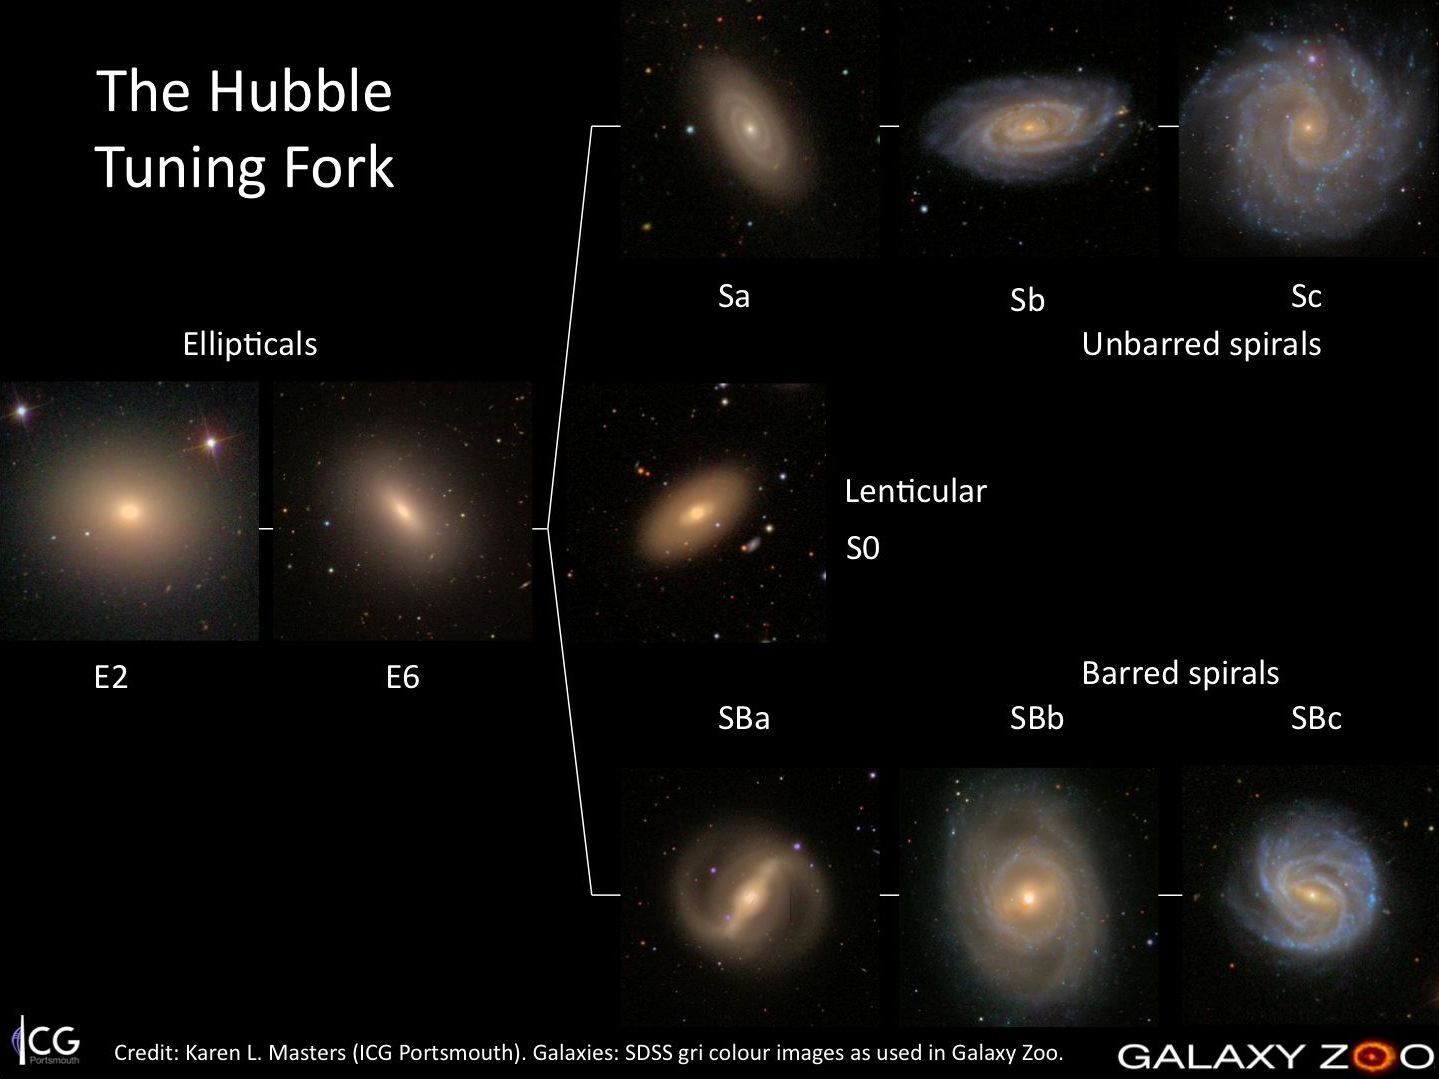
\includegraphics[width=0.95\textwidth]{Introduction/figures/hubble-tuning-fork.jpg}
    \caption{The Hubble tuning fork. Credit goes to the Galaxy Zoo collaboration (and specifically Karen Masters) for the creation of this figure. What was once thought of as an evolutionary track for galaxies, is now a widely adopted classification system for them based on morphology. On the left, we have elliptical systems - so called early-type galaxies - which are often `red and dead' systems. They have an intense merger history, which has destroyed their disk component and caused them to use the majority of their gas in star formation. On the right, we have two different kinds of disk galaxies. Ignoring the bar or un-barred part of this, they are systems which have a less intense merger history and have only accreted smaller systems into them. This serves to enhance their gas disk, and preserve their disk component.}
    \label{fig:hubble-tuning}
\end{figure}

Thus, as the merger rate has decreased through cosmic time, the survival of disk galaxies has increased. We, therefore, see two dinstinct populations of galaxies which can be easily defined by their morphology and colour which directly relates to their own evolutionary and merger history. One is of galaxies with a history of intense interactions with galaxies of equivilent mass, which lead to the complete destruction of their disks, and the other is of galaxies with a less intense merger history, with systems of much smaller mass than their own. These interactions and mergers serve to feed the gas within the galactic disks and increase their mass, while preserving the disk component of the system. In this thesis, I will not focus on merger rates any further than already explored. However, this whole discussion feeds into how we best identify mergers and interacting galaxies. I will, therefore, briefly discuss the morphology of galaxies and how it links into their properties. This will put things into perspective before I discuss how these systems are completely disrupted by merging and interaction. 

\section{GALAXY MORPHOLOGY \& GALACTIC PROPERTIES}
\noindent Galaxy morphology, and its change with time, specifically is the study and measure of a galaxies shape and features so that we can make different assumptions about it. There are many examples of morphological studies of galaxies. One of the largest to date was that of the Galaxy Zoo collaboration first published in \citet{2008MNRAS.389.1179L}. This project created the colour cutouts of $\approx$900,000 galaxies and presented them to citizen scientists for visual inspection. A citizen scientist is a volunteer who wishes to partake in answering scientific questions or annotating data in their spare time. Classifying nearly a million images by an individual is nearly impossible to do with any reasonable efficiency. However, in this project, nearly 100,000 volunteers stepped up to the task. Thus, each cutout could be visually inspected by different individuals who could make their own decision on the morphology of the galaxy. If enough individuals made a classification, one can then minimise the uncertainty in those classifications and find the answer from a group rather than leaving it up to an individuals opinion. Originally, this project made 40 million classifications across a range of morphologies. In the present day this collaboration has made hundreds of millions of classifications across a range of telescopes, redshifts and different morphology types.

The most important question asked in this - concerning morphology - is if the galaxy is smooth or a disk. As stated previously, this immediately gives an indication of multiple galaxy properties. First, if a galaxy is elliptical, it is likely that it is much redder than a disk galaxy \citep{1992MNRAS.254..589B}. Elliptical galaxies are dominated by their bulge component, meaning they are highly dispersion dominated and spheroidal in shape. As stated previously, this indicates a turbulent merger history, that has destroyed the ordered rotationally dominated component of a galactic disk. As a result of this, the gas mass and density are very low, having been removed by internal or external processes \citep{1976ApJ...204..365F}. As a result, the rate of star formation (or, more colloqually, the star formation rate; SFR) within these systems is very low - particularily when compared to disk galaxies. The gas within the galaxy has no opportunity to condense, fragment and form stars as required.

This low gas mass and low SFR within these galaxies has direct effects on their observable. The stellar populations that make up these galaxies are older and, therefore, lack the high mass and luminous OB-type stars that are typical of star forming regions. These stars are short-lived (only about a few hundred million years) and go supernova quickly in the history of these galaxies. The remaining smaller mass stars dominate the spectral energy distributions we observe of these systems. We can observe different parts of these distributions by using different filters on our telescopes. This leads us to defining a galaxies colour: the difference between the measured magnitude of flux in two different filters. Elliptical masses are often found to be red, in this system. We define red, in this context, as the difference between the `green' filter and the `red' filter (centered on 4,770$\AA$ and 6,231$\AA$ respectively). The green filter is designed to capture the part of the SED which is primarily contributed to by young or main sequence stars while the red captures that part from older, smaller mass stars \citep{Part of the SED we observe in each filter?}. Thus, when we subtract the magnitude observed in each filter, g-r, if this is very small we have a red galaxy and if it is very large we have a highly star forming galaxy. 

% Talk about the blue-ness of disk galaxies.
The opposite is true for galaxies which are primarily a disk. As stated previously, these systems have had a less tumultous merger history - particularily since z $\approx$ 1. An indicator of the merger or interaction history in disk galaxies is, in fact, the size and shape of the bulge component \citep{Bulge component is an indicator of merger history}. However, because of the plentiful gas, dust and ordered rotation in the galactic disk the SFR within is larger than elliptical galaxies. Gas clouds can condense and form throughout the galactic disk. It is well known that the surface density of molecular gas is directly related to the SFR throughout the galaxy \citep{Citing kennicutt, Schmidt etc}. Thus, the galactic disk provides the perfect environment for star formation. Spiral arms can exist in such galaxies, containing large filaments of gas and dust. They contain areas where large molecular clouds can condence, fragment and then collapse into new stars. These star forming regions will be young enough that massive OB-type stars will form, and be detectable to us. This increases the flux and magnitude found in the g band in our above equation. Thus, disk galaxies are often called `blue' galaxies, as the green value is much larger than the red in our colour observations.

\begin{figure}
    \centering
    \includegraphics[width=0.95\textwidth]{Introduction/figures/population-distribution.png}
    \caption{The distribution of galaxies in colour-colour space showing two distinct populations in a clear bi-modal structure. This is using the u-band and r-band filters and, therefore, the closer to 0 on the y-axis the bluer the galaxy. Left plot: the top population is the blue cloud, primarily composed of disk galaxies with young, star forming stellar populations. The bottom population is the red sequence, primarily composed of more massive elliptical galaxies which are gas poor and quiescent. Between these two populations lies the green valley, marked by the green lines. This is believed to be a transitional population moving between the blue cloud and red sequence for debatable reasons. To further show the split with morphology, the panels on the right split the colour-mass space into early-type (elliptical) galaxies and late-type (disk) galaxies. Note, this is Figure 2 of \citet{2014MNRAS.440..889S}}
    \label{fig:blue-red-population}
\end{figure}

% Now, talk about the blue and red sequence.
This gives rise to two distinct populations of galaxies: old, red elliptical galaxies and young, blue disk galaxies. When plotting colour-colour or colour-magnitude diagrams, these two populations are very clearly distinct with the `green valley' running between them. Figure \ref{fig:blue-red-population} shows the colour-colour distribution if the two populations. In this Figure, we clearly can see the blue population - blue cloud - and the red population - red sequance - beneath it with the green valley in between. The green valley is a disputed area of this distribution. Some works claim that it is a transition phase \citep{Papers green valley stuff. Start with Becky's work.}, where galaxies are moving between the two populations due to different processes, while others dispute this, and claim it is either a result of selection effects \citep{I think this is the red herring paper} or a different classification of object entirely \citep{Or this is the red herring paper}. However, what is definitive is that the rule of red galaxies are elliptical and blue galaxies are disk galaxies is not ubiquitous \citep{2022MNRAS.510.4126S}. Examples of blue ellipticals and red spirals do exist \citep{2022AJ....163..150K} and they are the subject of intense debate and study in the current field. However, as a general guideline for the expected properties of a galaxy the colour and morphology are deeply interdependent on one another.

% Want to introduce the idea of starburst galaxies, remnants and such here.
There are also many types of systems that do not fit this simple morphological definition of galaxies. Galaxies defined as starburst galaxies are often very morphologically irregular and have measured g-band fluxes, and therefore SFRs, far in excess of expectation for their mass. These then lead into post-starburst galaxies and merger remnants, who are the complete opposite and have very high measured r-band fluxes and therefore much lower SFRs. These are often called quiescent galaxies. These highly irregular systems have direct interplay, however, with their merger histories \citep{paper on post-starburst galaxies and merger remnants} and surrounding environments \citep{Paper on post-starburst galaxies and environment}. In fact, it has been found that in cluster environments, the fraction of disk galaxies drops to $\leq$10\% when compared to $\approx$60\% in the field.

The effect of the galactic environment on a galaxy should also not be understated. There are many ways to define the galactic environment, but it is most commonly associated with the number density of galaxies about them \citep{galaxy environment paper}. There are three broad classifications of environment: field, filament and cluster. A field galaxy is one with neighbours, and is in relative isolation. A filament galaxy has some neighbours, but their influence on the galaxy in question is minimal. A cluster galaxy is one in which a large number of other galaxies are bound in colossal galaxy cluster structures. In these environments, SFRs are suppressed \citep{Paper on environmental suppression} by ram pressure stripping and galaxy morphology is highly irregular due to constant interaction and merging. In these environments, the relation between galaxy morphology and the underlying processes is almost completely broken by interference from the environment.

Thus, galaxies in the field or in filaments are of particular interest. Here, we can study the direct link between morphology and the underlying processes of galaxies. And these, in turn, are highly dependent on galaxies underlying merger and interaction histories. So, what is this relation? As stated previously, the influence of interaction and merging accelerates the evolution of rotational systems to dispersion dominated systems. However, there are many more subtle affects that can be attributed to galactic merging and interaction. For instance, if two galaxies can be brought into a state of starbursting due to merging \citep{Paper on starbursting galaxies in interaction.}. This completely changes the underlying SED of the galaxies involved, and can lead to the rapid quenching both systems \citep{Paper on quenching a galaxy with interaction}. Thus, depending on when we observe such a galaxy, we can find either a much bluer or redder galaxy than expected. However, it can also be found that such interactions do not lead to much change in the underlying SED at all \citep{Paper on not much change in the SED of a galaxy}. So, why is this? It transpires that the effects of a galaxy merger or galaxy interaction are dependent on the underlying parameters of the galaxies themselves. This leads to us having multiple classifications of galaxy interactions which each lead to different outcomes for the galaxies involved. 

\section{CATEGORISATION OF MERGERS}
\noindent The effects of galaxy interaction and merging is dependent on multiple different factors and underlying parameters. However, the two most important parameters are the mass ratio \citep{paper saying mass ratio is important} and gas content \citep{paper that says the gas content is important} of the galaxies involved. The impact parameter also does have a lot of influence over the final morphology over the system, however, we will discuss this further in the next section. The recognition that the mass ratio and the gas content of interacting galaxies leads to significant outcomes means that a small categorisation system has been produced to recognise the different kinds. For the mass ratio, we define a major, a minor and a micro interaction \citep{Paper with these definitions in them?}. These are the ratios of the primary galaxy mass (the more massive galaxy) and the secondary galaxy mass (less massive galaxy). These are then further sub-divided into two seperate categories based on their gas content: a wet merger or a dry merger \citep{Paper on wet vs dry mergers}. This refers to the gas mass and colour of both galaxies. A wet merger involves lots of gas in the two galaxies colliding, and therefore, lots of resultant star formation. Both of the involved galaxies are blue, and often disk-dominated galaxies. A dry merger involves little gas, and is often the merger of massive, red elliptical galaxies. There are also intermediate categorisations based on the amount of gas, such as damp mergers (where there is some gas, but not enough to completely dramatically increase star formation) and mixed mergers (mergers between gas-poor and gas rich systems) \citep{Paper on mixed / damp mergers}, however, we focus on the binary definition of wet and dry mergers.

Depending on the classification of an interaction leads to specific outcomes for the interacting galaxy system. A major interaction is when the galaxies involved have a mass ratio of approximately 1:1. Some definitions vary, however, and allow this limit to go down to 1:3. For the purposes of this work, they must have a mass ratio of approximately 1:1. Major interactions are the most devastating to the morphology of the systems involved, with the forces upon them causing severe morphological distortion and the formation of tidal features (more on this in the following section). If the two systems merge, there is complete destruction of the disks in both galaxies and the post-merger remnant will be highly irregular. If this major interaction is also a wet one we would also expect a significant increase in the SFRs of both galaxies \citep{Increases in SFR in wet interactions} - this is particularily true if the two systems actually coalesce \citep{Papers on increases in SFR in coalesced mergers}. We also find that wet major mergers have an increased AGN fraction \citep{Paper on wet major mergers and AGN}, which suggests that such a merger may play a role in nuclear ignition. The opposite of this is true when a major interaction is dry, where only a small increase in SFR is found in the nuclear region of the galaxies \citep{Papers on dry mergers leading to increased SFR in the nuclear region}. This holds true even when the two systems actually merge, with no significant change in SFR or AGN fraction emerging at all.

\begin{figure}
    \centering
    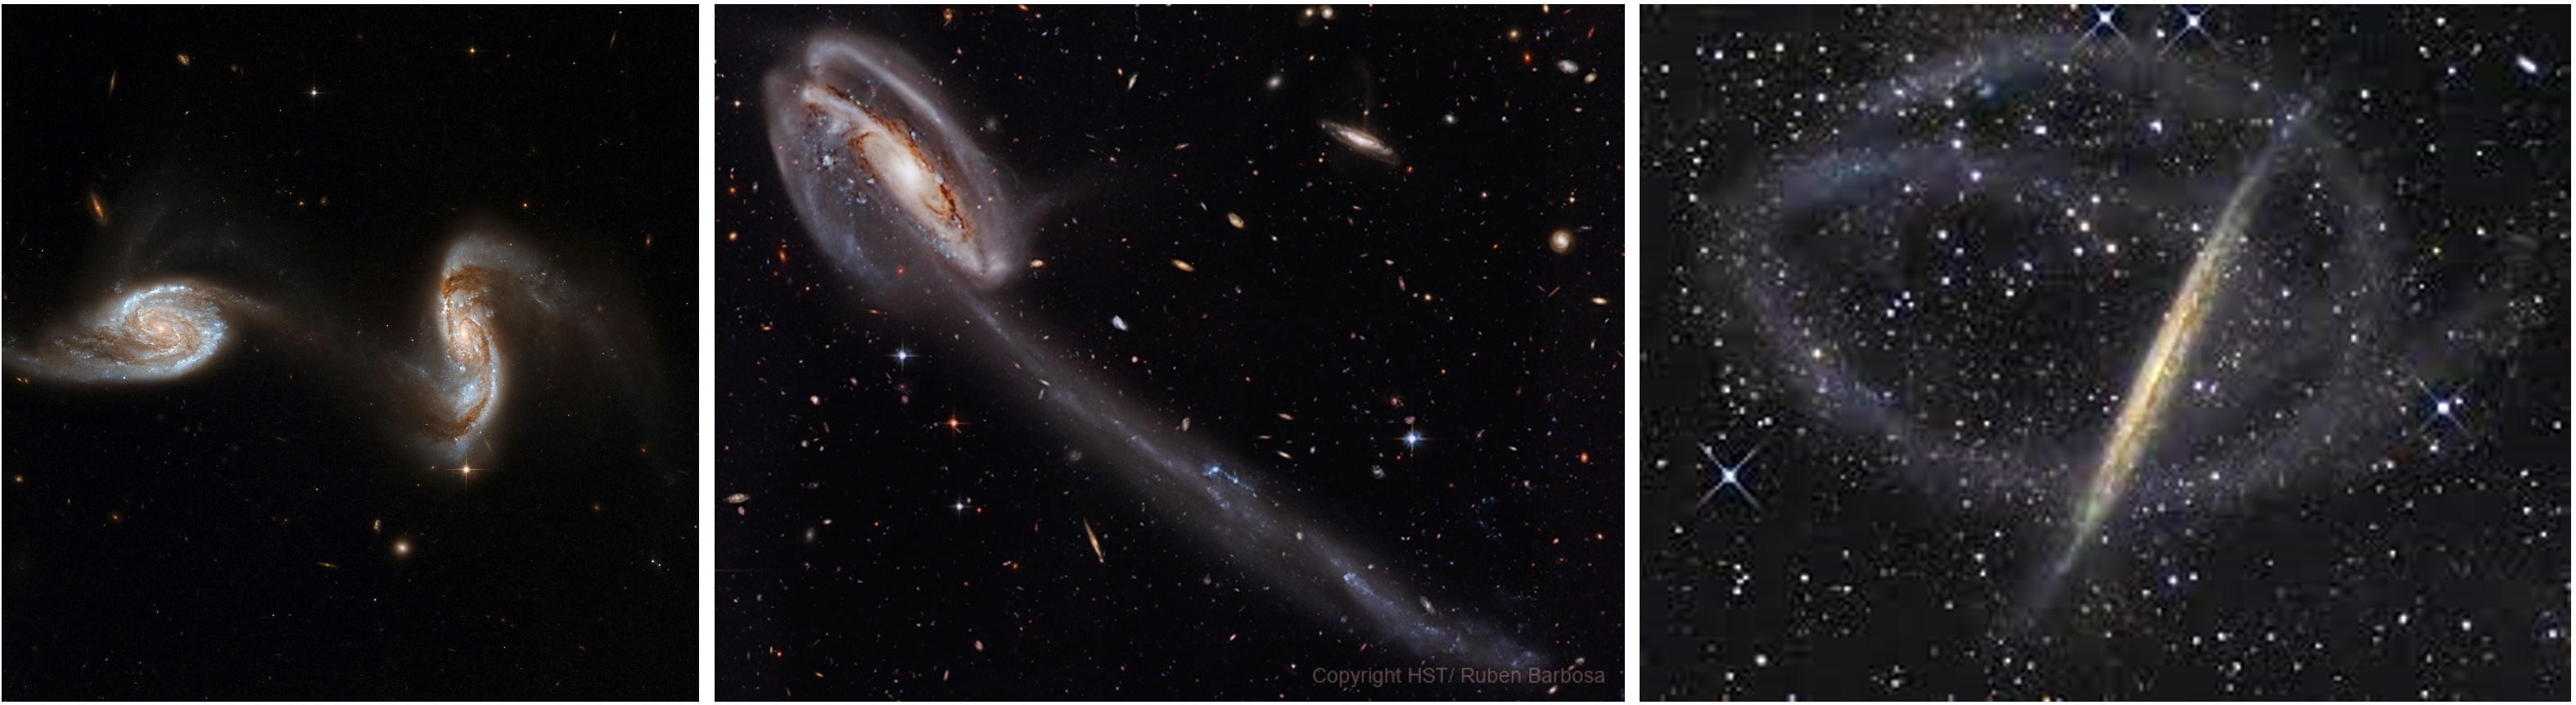
\includegraphics[width=0.95\textwidth]{Introduction/figures/combined-examples-mergers.jpg}
    \caption{Examples of a major, a minor and a micro interaction. Each of these are wet interactions, containing lots of gas and therefore increases in star formation. These are the Arp 240, Arp1 188 and NGC 5907 systems, respectively. Here, we show the famous double looped stellar stream of NGC 5907 but point out that the existence of the second loop is in dispute and that we only show it here for illustrative purposes. From major to micro interactions, we see decreasing impact and change in the morphology of the primary galaxies but always the complete destruction of the secondary.}
    \label{fig:merger-clsfs}
\end{figure}

A minor interaction has less catastrophic consequences for the morphology of one of the two galaxies. This is defined as an interaction where the mass ratio is less than 1:1 but greater than 1:10. Due to this large mass disparity, the morphology of the primary galaxy is relatively unaffected by such an interaction. However, the secondary galaxy will be almost completely destroyed by the encounter. If it is only flying by in an interaction, the secondary will be higly disrupted, forming a long and stretched tidal tail as it moves through the orbit. This will leave a large stellar stream around the primary galaxies disk, which can become a probe of the dark matter halo about the galaxy. In a wet merger, the tidal tails formed in the secondary galaxies can often condense into their own tidal dwarf galaxies \citep{Papers on tidal dwarfs}. This leads to interesting, dark matter-less systems that we can explore and test alternative theories of cosmology \citep{Papers on MOND and that sort of thing}. When these systems actually merge, we observe small increases in the SFR of the primary. There is ongoing work investigating whether such mergers were actually a primary driver of star formation in galaxies across cosmic time \citep{Sugata's paper on the work} with contradicting results \citep{Papers with minor interactions being primary drivers of cosmic SFR}.

Finally, a minor interaction is one in which the mass ratio between the primary and secondary galaxies is less than 1:10. This always sees the complete destruction of the secondary galaxy, whether just a flyby or a complete merger. A very local example of this is the interaction of the satellite galaxies of the Large and Small Magellanic Clouds \citep{Papers that say the LMC and SMC are examples of micro mergers}. These also form many stellar streams about their primary galaxy and are often absorbed by the primary with very little change in its morphology. Therefore, it has been theorised that such mergers could be a much larger driver of cosmic star formation through time but leaving very little evidence or impact on the primary galaxy. 

Figure \ref{fig:merger-clsfs} show examples of each of the different merger categories we have defined here. These, from left to right, are the Arp 240, Arp 188 and NGC 5907 systems. They each show a major, minor and micro interaction, respectively, and demonstrate the change in effect the mass ratio has on the morphology of the galaxies involved. From Arp 240, with the complete destruction of the galactic disks and formation of tidal features to NGC 5907 where the primary galaxy is barely disturbed at all. Thus, the different categories of interactions and mergers have very different impacts on the systems involved. I will now discuss, in depth, the effects that interaction has on these galaxies and specifically explore the formation of morphological disturbances like tidal features, changes in the SFR and the increase in AGN fraction.

\section{EFFECTS OF GALAXY INTERACTION}
% Here, present examples of interacting galaxies and the context in which we're talking about them.
The idea of two or more galaxies interacting and the effect that it would have had upon galaxy formation and evolution was thought to be minute \citep{Found this info in Chapter 8 of Binnie and Tremaine. Need to find a better source!}. We now understand that galaxy interaction plays an important, and fundamental role in the evolution of galaxies. As stated previously, they have multiple affects upon the systems undergoing the interaction. The specific effects of interaction lies on a host of parameters, we have discussed the mass ratio and gas content and mentioned the impact parameter but there is also the orientation of the interaction, the relative sizes of the galaxies and the point in the dynamical history of the interaction we are observing \citep{Some review paper, perhaps that states that these parameters are important}. Thus, in this section, we will explore how these different underlying parameters link to the physical processes we observe in interacting and merging galaxies.

% For each of these sections below, I want to do a deep dive on how each process is driven. Will maybe mention simulations throughout, but we shall see?
\subsection{Morphological Distortion: Tidal Features}
% Introduction here: What do I mean by tidal distortion? What are we actually looking at?
\noindent It is important to start here with pointing out that galaxies are large gravitationally bound systems of stars, interstellar gas, dust and dark matter. Upon a close encounter between two galactic systems, these components experience strong gravitational forces which disrupt their ordered layout. AS the galaxies move rthrough their relative orbits, the gravitational potential changes at an accelerating rate. This imparts energy into the ordered components of the galaxies, and caused thermalization of their internal motions. This leads to violent relaxation, where the stellar orbits are so altered they no longer follow their prior orbits. However, the energy in the system must be conserved. Thus, as the internal stellar motions within the galaxy gets thermalized, the energy in the galaxy's orbits decay via dynamical friction. If this decay is large enough, the energy in the galaxy's orbit may be sufficiently reduced to no longer escape from one another and they will eventually coalesce to leave a single merger remnant. 

However, before this, the changing graviational fields as the two galaxies encounter each other leads to radial distortion of each galaxy. This leads to the drawing out of galactic material into long plumes which can eventually become tails. If stellar material, including gas, dust and stars, is close to the edge of the galaxy a combination of the galactic rotation and radial elongation lead to it being sheared off and away from the galaxy. This forms two `tidal tails` in the system, one leading and one proceding the motion of the galaxy. Dependent on the geometry of the encounter, the trailing tail of one galaxy and the preceding tail of the other can form a `tidal bridge' - a linking of the two systems. An example of both of these is the interacting pair Arp 240, shown in left hand plot of Figure \ref{fig:merger-clsfs}. 

The geometry of the bulk motion of the galaxy is very important in forming these tidal features. As the internal galaxy rotation and bulk motion in of the galaxy's orbit in the encounter must match for this shearing of material to occur. Thus, the formation of tidal tails and tidal bridges is only possible in a prograde interaction whereas a retrograde interaction suppresses them \citep{Papers on prograde and retrograde interactions}. Further, depending on the relative velocities in of the galaxies these tidal tails can be split off from the galaxy as the encounter continues. This can lead to the formation of `tidal debris' of stellar material forming about the galaxies. In some instances, this tidal debris can actually coalesce and form galactic systems of their own \citep{Papers on tidal dwarfs and need to actually proof this is a thing}.

While the most striking tidal features to form in galactic encounters are these tidal tails and bridges, we also see the formation of a slew of other features. These include `stellar streams' (previously discussed), shells and rings forming in the galactic disk. As stated, stellar streams are likely smaller galactic systems that have been destroyed while passing the primary galaxy. This leaves a faint stream of material about the galaxy. The right plot of Figure \ref{fig:merger-clsfs} shows an example of a stellar stream with the NGC 5907 system. Shells, on the other hand, are formed about galaxies and can be present in as many as 30\% - 50\% of elliptical and lenticular galaxies \citep{Shell presense in galaxies}. The left panel of Figure \ref{fig:tidal-features-ex} shows an example of shell in the elliptical galaxy NGC 1344. Spectroscopy shows that shells are primarily composed of stars. There are often numerous shells in a single galaxy, although most often we only detect $\approx$3. Shells are formed from the disruption of a small satellite around a significantly more massive galaxy - so, in a minor to micro interaction. This then forms a stellar stream, which overtime condenses to a cloud of stars orbiting the primary galaxy. This then either forms into an X-shaped structure or a annulus which, in the 2D projection of the sky, appears as a shell. Thus, observing a stellar stream or a shell is highly dependent on the time in the dynamical history of the encounter that we are observing.

\begin{figure}
    \centering
    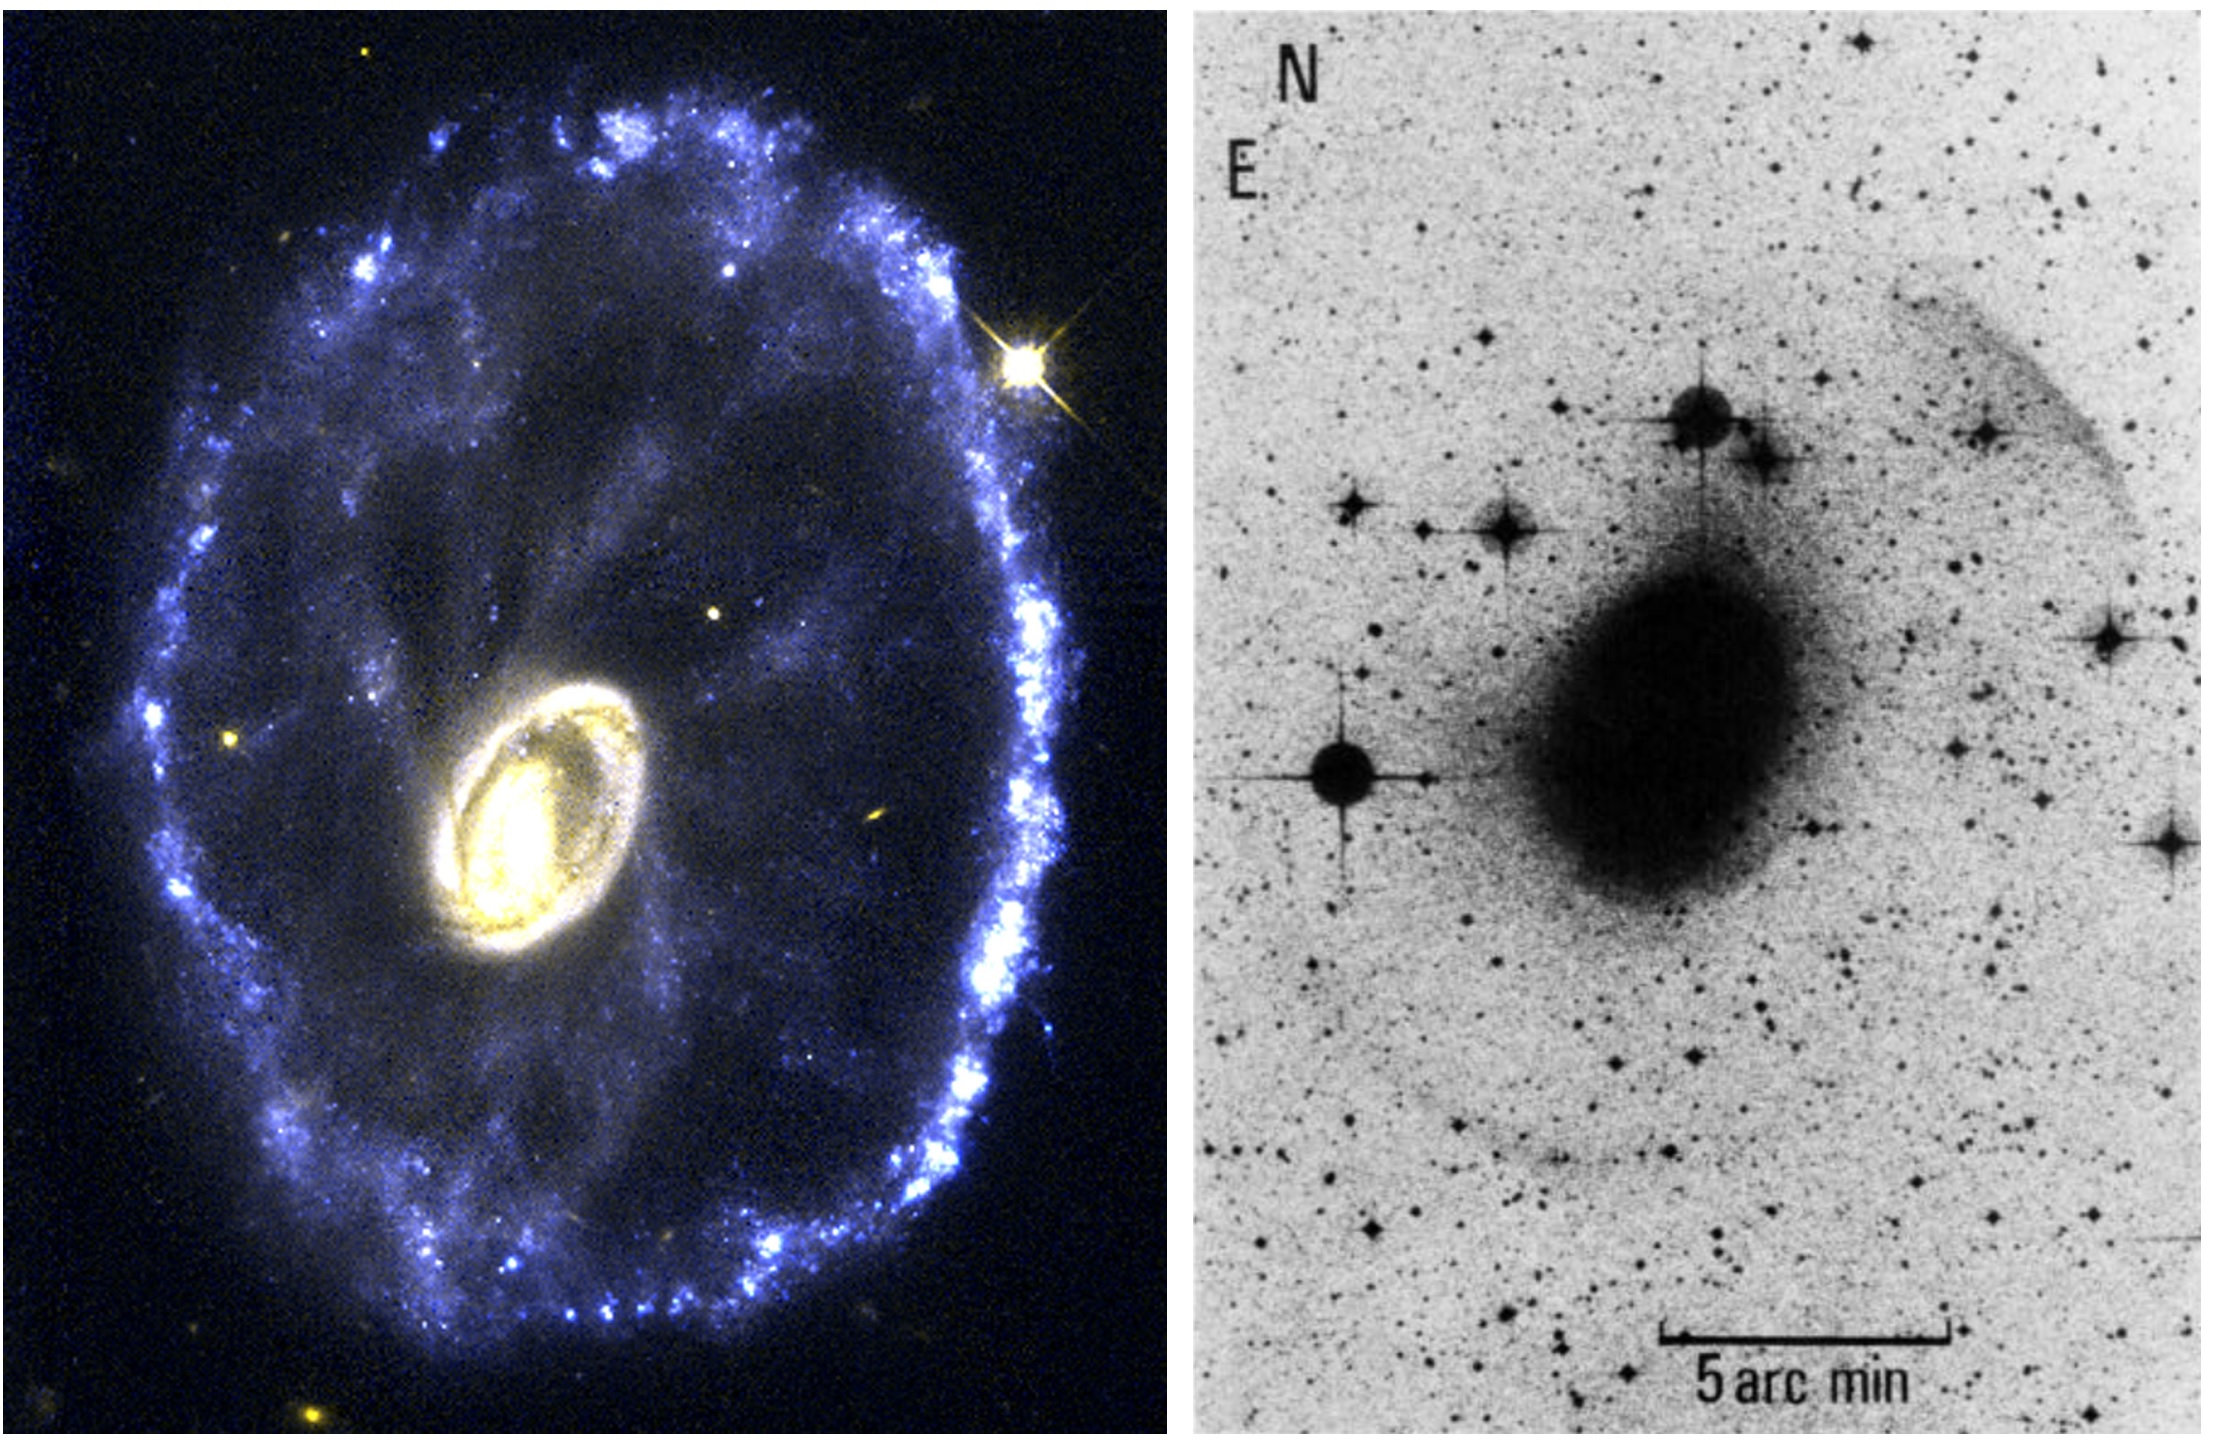
\includegraphics[width=0.95\textwidth]{Introduction/figures/shells-rings.jpg}
    \caption{Examples of a collisional ring galaxy and a system containing shells. Left: The Cartwheel galaxy, the most famous ring galaxy to date. Ring galaxies can only formed by a direct, head on collision between two galaxies. The ring itself is composed of a region of the disk undergoing intense star formation due to the density wave passing through the disk from the impact of the secondary galaxy. Right: The system NGC 1344, showing two shells of stellar material about it. This is formed by the condensation of stellar streams into clouds of stars. Cartwheel Galaxy Image: NASA / Hubble, NGC 1344 Image: \citet{1983ApJ...274..534M}}
    \label{fig:tidal-features-ex}
\end{figure}

Finally, we find rings can form from galaxy interaction. These systems are often called ring galaxies or collisional ring galaxies. Figure \ref{fig:tidal-features-ex}'s right panel shows the Cartwheel Galaxy: a famous example of a ring galaxy. This ring is formed of young, hot stars and is formed only from the head-on collision with another system \citep{Lynds and Toomre 1976}. The interaction to form this is so intense, that it causes a density wave to pass through the galactic disk which triggers intense star formation at its wake. These systems are incredibly rare, as this requires an impact parameter of 0 for this feature to form.

From the example of a ring galaxy, we see that interaction not only affects the stellar distribution of the galaxy, but also has direct impacts on the gas within it. As I have stated in previous sections, interaction and merging can induce enhancements in star formation and even lead to a starburst in a galaxy which brings about the complete quenching of the system.

\subsection{Star Formation Enhancement} 
\noindent As stated previously, it is often observed in interacting and merging galaxies that the star formation is enhanced in some way. While to what level this enhancement is often debated between observations \citep{} and simulations \citep{}, the underlying processes that lead to enhancement is well understood. First, by star formation enhancement we mean that the SFR either globally or in different regions of an interacting galaxy is higher when compared to isolated galaxies. Thus, some property of interaction is causing an increase in the star forming activity of the galaxies involved. 

The rate at which stars form is known to be directly related to the surface density of gas at any given piont within the galaxy. The global version of this idea is the Schmidt Law \citep{1959ApJ...129..243S} and finds a tight correlation between these two parameters like so:
\begin{equation}
	\Sigma_{SFR} \propto \Sigma_{Gas}^{n}. 
\end{equation}
Following from the realisation of this relation, \citet{1989ApJ...344..685K} found in nearby disk galaxies that n $\approx$ 1.3, and related it between the surface area density of gas and SFR. It is therefore easy to see that due to an interaction the torques and gravitational forces upon the gas clouds within each galaxy causes them to lose angular momentum. This loss in angular momentum causes the gas clouds to drift inwards, towards the galactic core. As more gas clouds fall into the core, the surface density of gas in this region is driven up rapidly. This in turn drives up the SFR dramatically.

While this is a simple explanation, and an easy idea to hold about driving the increase in star formation in interacting galaxies, it is not the whole picture. Increases are also detected in the tidal features and the disturbed disk of them as well \citep{Papers on increases in star formation in the galactic disk?}. So, what drives these? In fact, it is the same basic principle, except due to the distortion of the disk itself. As the morphology of the disk is compressed into a tidal feature, we see the same increase in the surface density of gas which leads to a further dramatic increase in the SFR. However, this is much more sparesly populated about the galaxy than expected \citep{What am I even saying here?}. Thus, depending on when in the dynamical time we observe the galaxy will heavily affect if we see any enhancement in star formation at all. It is dependent if enough time has passed for the angular momentum in the gas to be lost and for it to move into the galactic core, and areas of significantly increased surface density \citep{Seriously, am I even making any sense here?}.

This movement and compression of gas into the galactic centre also has a serious significant effect. It can lead to the feeding of the supermassive blackhole at the galactic centre \citep{Movement of gas to galactic centre causing AGN}. This, then, causes ignition of the supermassive black hole and us to observe an AGN in the galaxy.

\subsection{Ignition of Active Galactic Nuclei}
\noindent The presence of an AGN in a galaxy is often very hard to miss. When we view them face on, the AGN is so luminous that it often outshines the entire bulge and disk of the galaxy. Thus, to study the galaxies they are present in we must carefully remove all contribution of the AGN to the underlying SED flux. The bright flux we observe is from a long and complicated process of accretion of material onto the supermassive black hole at the galactic centre \citep{Paper on what an AGN actually is}. The structure of material about the black hole is also complex, and results in many observational oddities. 

An accretion disk of material that is directly rottating about and orbiting the black hole structure exists. As the material accretes, it causes the SMBH to project large, powerful jets of radiation perpendicular to the accretion disk plane. These jets are highly luminous, and are what we observe in the optical, infrared and X-ray. There has been discovered two populations of AGN: containing narrow and broad emission lines, named Seyfert 1 and Seyfert 2 AGN respectively \citep{Paper on Seyfert 1 vs Seyfert 2 galaxies}. While, at first, thought to be two distinct types of AGN, there has now been a significant push to unify these AGN into one population. This unified population is related to the structure of material surrounding the accretion disk and the inclination of the galaxy.

About the accretion disk, there is a torus of material.This material is dusty, and highly absorbing of the emission from the SMBH-accretion disk system. This leads us to only observing narrow line emission (Seyfert 2) when we observe the AGN through the torus and observing both narrow and broad lines of emission not viewed through the torus. Figure \ref{fig:agn-structure} shows the underlying structure of an AGN system as described here. As we move to higher luminosities, we get further populations of AGN such as blazars, quasars, radio-quiet and radio-loud systems. These are all dependent upon the inclination at which we are viewing the AGN system and the material in the line of sight.

%\begin{figure}
%    \centering
%    \includegraphics[width=0.95\textwidth]{Introduction/figures/}
%    \caption{}
%    \label{fig:agn-structure}
%\end{figure}

Due to the range of characteristics and emissions an AGN can have, we therefore have multiple methods of detecting them. First, we can use Baldwin, Phillips and Terlevich (BPT) diagrams to identify AGN from well measured emission lines. These act by measuring lines such as OIII, OII, NII and H$\alpha$ lines and comparing their relative flux. By using well defined cuts in these parameter space \citep{Paper that gives those cuts. It's Kennedy and Ho or something like this}, it is possible to identify a galaxy as AGN. As we move to higher lumionosities and AGN in the X-ray or radio, we can define specific luminosities at which an AGN is likely. In radio, this is quite complex and contributions from H$\alpha$ regions and star formation must be accounted for \citep{Paper on radio AGN identification}. Whereas, in X-ray, we can simply make cuts in the luminosity space above which only something as powerful as an AGN could produce such luminous X-ray emission \citep{Paper on X-ray emission}.

Thus, from this description of an AGN structure and the methods of detection, it is perhaps easy to see how galaxy interaction increases the probability of nuclear ignition. AGN require large volumes of gas and dust to be present at the galactic core; a surge of which interaction provides. However, what is often surprising from observations of samples of interacting systems is the meagre increase in the AGN fraction within them. There have been many hypothesis as to why this might be, from a delay in the AGN ignition \citep{Paper on delay in AGN ignition, probably Ellison 2011} to AGN flickering \citep{Paper on AGN flickering}. A delay in AGN ignition would make sense, again, in the context of the structure we have just discussed. As gas and dust are moved into the galactic core, they do not necessarily immediately move dierctly around the SMBH and may take time to get there \citep{Paper on why delay might happen}. There may be other mechanisms at work within the AGN itself that causes suppression of igntion for some time \citep{Paper on AGN mechansim being why delay could happen}. This could also produce the AGN flickering, where material may be cutoff from the SMBH and cause the AGN to turn on and off. This could be further proved if it was found that the AGN fraction varied across the dynamical time of interaction.

Iit cannot be disputed that the sudden movement of gas into the galactic centre during interaction does, indeed, seem like an obvious way for activation to occur. However, as gas is removed from the galactic disk from either movement or star formation, we see the beginning of quenching in the galactic system. 

\subsection{Quenching of Galactic Systems}
\noindent Through a galaxy interaction, as discussed, there is significant movement in gas, AGN activation and large increases in star formation across the galaxy. However, this comes at a cost. A galaxy only has a limited resevoir of gas available to it. Therefore, this sudden increase in gas usage in multiple different processes leads to the gas being used in a significantly shorter timescale than expected. Once the gas is used, star formation and AGN will rapidly cease and the colour of the galaxy will change from highly blue to highly red. 

This rapid quenching of systems is different to what is expected in the field. Galaxies gradually use their gas over long periods of time forming stars and slowly quench as the average gas density across the disk reduces to the point of very low SFRs \citep{papers on regular quenching}. However, by concentrating gas and increasing the gas density in an interaction, even if a galaxy had stopped forming stars previously it is able to increase in star formation again and use the remaining gas entirely. Thus, we often seen increases in the SFR during and immediately after an interaction but then the sudden shut off of SFR shortly after it \citep{Paper on sudden shut down of SFR by interaction}.

\section{IDENTIFYING INTERACTING AND MERGING GALAXIES}
\noindent I have described and explored the effects of interaction and merging across the galaxy population. I have described the basis of galaxies, and how these are then changed and what we expect to see when we observe interacting galaxies in comparison. However, we are only able to so fully understand these differences by using large samples of interacting galaxies and comparing them to large control samples.

The first samples of interacting galaxies were identified by eye. The earliest interacting galaxy catalogue was the \citet{Arp catalogue} of Atlas of Peculiar Galaxies. This contained 166 interacting systems. This was quickly added to with a 2-part edition of the Vorontosov-Velaminov catalogue \citep{Both parts of the VV catalogue}, providing a further 268 systems to the original \citet{Arp} catalogue. Both of these catalogues contained only the most major interactions, where clear tidal features easily put them into the interacting galaxy classification. The tidal features of these systems were used to classify them by eye, meaning they were only capturing a specific part of the dynamical timescale. These samples were also not large enough to make statistical, representative statements about the interacting galaxy population. Thus, larger catalogues had to be created.

Catalogues made later than the previous examples also often used visual classification to find interacting and merging galaxies. The previously mentioned Galaxy Zoo collaboration created a catalogue of 3,003 interacting galaxies which were identified by citizen scientists based on morphology \citep{Darg et all. paper}. However, a limitation was found when visually classifying galaxies at different parts of the interaction timescale. With no information on the redshift, and therefore 3D distribution, of galaxies within images it was very difficult to distinguish `close pairs' from truly interacting pairs. A close pair, in this context, is two galaxies which appear to be very close together in the sky in the 2D projection of the sky but are actually at different redshifts. This means they are not actually close together in 3D space and cannot possibly be interacting. Many interacting galaxies created by visual classification have to throw away masses of false positives from their sample \citep{Papers saying large numbers of interacting galaxies are removed.}. As machine learning algorithms began to be used in galaxy classification, this problem spilled over.

Neural networks have began to play an increasingly central role in galaxy classification. As the size of observational samples have increased explonentially, so has the apparence of the impossibility of visually classifying each galaxy individually. Rather, a neural network can now be trained to make morphology classifications of galaxies using a much smaller subset of visually classified galaxies. A neural network is a layered structure of interconnected nodes which can pass information to one another. Each node has a weight assigned to it which allows it to alter the input and then pass on the weighted output. The input in this context can be some information about a galaxy, a section of an image or an underlying parameter estimation. These nodes all interconnect through many different layers where they all perform operations on some input. These operations all then come together in a final classification layer at the end which outputs either a formal classification or some value that can be mapped to a classification by a user.

A formal classification can be made in this way by training the neural network to recognise certain features of an image. Training a neural network in supervised learning involves providing it with a training set of fully annotated data so it can `learn' classifications form examples. To train the neural network iterates through the provided training set and makes classifications upon each input. It then checks how many it got right and how many wrong, and then tweaks the weights applied to each node throughout it. It then makes the classifications again and checks whether it got more right or wrong. By doing this through many epochs of the training set, it gradually tweaks its internal weights such that it should be able to make the same classifications on an unknown dataset and recognise images with similar classifications to the training set. Thus, it is important that the training set is large and is representative of the full parameters space a user wishes to classify.

In morphology classification, the workhorse neural network is the convolutional neural network (CNN). A CNN takes an image and breaks it down into smaller subsections in a convolutional layer. These smaller subsections - essentially arrays directly from the image - are passed through normal neural network operations and activations and are altered by the weights at each node. Depending on the number of layers in the CNN, the image may be sub-divided, convolved and weighted many times before being fed into a classification step which outputs the final classification. The real power of a CNN such as described is that it is able to recognise features in an images. For instance, spiral arms, tidal features or ellipticals. 

However, using a pure CNN for the purposes of identifying interacting galaxies still introduces the same problems as using visual identification. While it is able to recognise the morphology of interacting galaxies, or recognise two galaxies that are close together it cannot discern this from close pairs. Thus, many works have been done using CNN to identify interacting galaxies and have then had conduct large-scale de-contamination of their final samples \citep{Papers removing contamination of interacting galaxies}. Often, doing so leads to reducing potential sizes of interacting galaxy samples by 50\% - 75\%, with the de-contamination processes requiring visual inspection or further ancillary data which is time consuming to conduct or attain.

New methods combining machine learning with something else have come about in order to overcome this issue. Some works have turned to using the underlying observational parameters of the galaxies to define them \citep{LDA paper}. Others have turned to estimating ancillary parameters in different ways in an attempt to reduce initial contamination \citep{Papers with estimating redshifts}. Many works initially attempted to train CNNs on simulated data; where the training set could be controlled and composed of the entire dynamical time of interaction and be completely empty of contamination. However, when applied to observational data it was found that the accuracy of such models completely breaks down \citep{Papers on simulated to observed data in neural networks}.

Thus, the identification of interacting and merging galaxies in an automated fashion remains an open question. Spectroscopic or photometric information for many potential systems does not exist, and therefore cannot be discerned from close pairs. In this work, we present a new way of finding interacting galaxies using a combination of representation learning \citep{Representation learning} and visual classification. But that is discussed in Chapter 2.
\chapter{Advanced PySPAM: An Infrastructure to Constrain Underlying Interacting Galaxy Parameters}\label{chapter4}
\section{Introduction}\label{Introduction}
% Introduce interaction, and why it's important.
\noindent The precise interplay between the observed processes we have discussed in this thesis and the underlying physical parameters of the involved galaxies is difficult to quantify. Using large scale observational datasets allows us to probe this relation, but without the ability to constrain the dynamical timescale the precision of our constraints on it remains limited. Algorithms have been developed to match the underlying parameters of an interaction and its dynamical timescale by directly modelling the expected final morphology. If a simulation of an interaction can reproduce the final morphology, then it has likely correctly inferred the interaction over the dynamical time.

Examples of algorithms designed to make this matching include Identikit by \citet{2009AJ....137.3071B} or the Stellar Particle Animation Module (SPAM) by \citet{1990AJ....100.1477W}. However, finding the best fit underlying parameters for more than a handful of systems is often seen as unfeasible. There are often greater than 10 different parameters which contribute to different observed morphologies. This leads the underlying parameter space to be greater than 10-dimensional and complex. Exploring even a sub-space of this parameter space fully requires tens of thousands of models to be run. This is also hindered by its degeneracy. For example, \citet{2010ASPC..423..227S} found that four of their best-fit models were able to accurately match morphology of the Arp 284 system. Therefore, it is often preferable to use large cosmological simulations \citep[e.g.][]{2015MNRAS.446..521S, 2018MNRAS.480..800H, 2020MNRAS.493.3716H} to create large samples of synthetic interacting galaxies where analogues to the observed system can be found. This, however, limits our capability to explore observational parameter space beyond the limitations of such cosmological simulations. By their nature, cosmological box simulations have finite scope and size; meaning the rarest (and likely most fundamental) interacting systems will remain unexplored without significant further computational expense.

This limitation of directly comparing numerical simulations to observations was solved in a novel way by \citet{2016MNRAS.459..720H} in the Galaxy Zoo: Mergers (GZM) project (for details on Galaxy Zoo, see \citet{2008MNRAS.389.1179L}). GZM worked with citizen scientists to run simulations of interaction and visually compare the simulated morphology to observations. GZM studied a sample of 62 interacting galaxies from the Arp catalogue of interacting galaxies \citep{1966ApJS...14....1A}. Citizen scientists' were given a selection of simulation outputs around an observation and would select the one which appeared most alike. The simulations would then be run again with tweaked underlying parameters with the citizen scientist selecting the new the best fit output. With enough citizen scientists on the project, enough new simulations run and enough time GZM were able to find the best fit parameters for their interacting galaxy sample across a 14-dimension parameter space. This created the largest fully constrained interacting galaxy samples to date. In the era of the Vera C. Rubin Observatory such an approach will not be practical, with statistically significant samples of thousands of interacting galaxies potentially being produced every week, a new approach is required.

In this Chapter, we present an automated methodology to constrain the underlying parameters of interaction. We combine a fast restricted numerical simulation code with a Markov-Chain Monte Carlo (MCMC) framework. We apply this over a 13D parameter space and constrain the probability distribution and find the likely parameter values describing an interacting galaxy system. This approach allows us to marginalise over each parameter, provide the best fit value as well as the error on each measurement. First, we apply this to a set of synthetic interacting galaxy observations created from a restricted N-body simulation where we have input the 13 underlying parameters. This provides us with diagnostics of our methodology. We then apply our process to five real observations of interacting galaxies and discuss how our methodology could be applied to real data, and the limitations therein. We also discuss the more general limitations of this approach, with a particular emphasis on the computational expense required, and the potential future solutions.

% Layout of document/
The layout of this Chapter is as follows. In Section \ref{Data}, we describe the sample of 51 galaxies we will study and our approach to observation preparation. Section \ref{Methods: sims} will summarise our simulation code and how it has been updated from previous iterations. We also describe how we build our sample of synthetic interacting galaxies and the parameter space we will explore with this simulation. A full discussion of our results will be given in Section \ref{Results} followed by our conclusions and future work in Section \ref{Conclusions}.

\vspace{-5mm}
\section{Data}\label{Data}
% What is the data?
\subsection{Sample of Major Interacting Galaxies}
\noindent In this work, we test our Markov-Chain Monte Carlo (MCMC) process on idealised, mock observations of 51 major interacting systems. These mock observations are created using our numerical simulation where we have input the underlying parameter values directly. As we know what the true underlying parameters of each interaction are, we can test the accuracy of our MCMC. To create these mock observations, we use the underlying parameters found in the GZM project for 62 interacting galaxies.

Of the 62 systems, we create synthetic images of 51 of them to act as our idealised observational sample. As we are including the flux distribution of each system, we require an accurate redshift of each system. 3 of the 62 systems do not have a redshift measurement in the NASA Extragalactic Database (NED), the Sloan Digital Sky Survey (SDSS) or Simbad databases. Therefore, we discard these. We create each mock observation as though it was observed using SDSS. Of which, a further eight systems are not present. Therefore, we also discard these systems. This leaves us with the GZM best-fit parameters of 51 systems with which to create our synthetic observations. The details of the real systems are displayed in Table \ref{tab:Objects}, including the target coordinates, the SDSS ID and the redshift measurements we use. How we create our synthetic images is described in Section \ref{sec:syn_sample} after we have described our simulation.

\begin{table*}
    \centering
    \resizebox{0.79\textwidth}{!}{\begin{tabular}{|c|c|c|c|c|c|c|}
    \hline
         Name & SDSS ID & RA & Dec & Redshift \\
         \hline
         Arp 240 & 587722984435351614 & 204.980417 & 0.835278 & 0.02250 \\
         Arp 290 & 587724234257137777 & 30.946317 & 14.72365 & 0.01171 \\
         Arp 142 & 587726033843585146 & 144.429583 & 2.763056 & 0.02329 \\
         Arp 318 & 587727177926508595 & 32.380516 & -10.158508 & 0.0132 \\
         Arp 256 & 587727178988388373 & 4.710417 & -10.369167 & 0.02730 \\
         UGC 11751 & 587727222471131318 & 322.247796 & 11.382539 & 0.02909 \\
         Arp 104 & 587728676861051075 & 203.037083 & 62.733889 & 0.01082 \\
         Double Ring, Heart & 587729227151704160 & 238.287292 & 54.147861 & 0.040 \\
         Arp 285 & 587731913110650988 & 141.040000 & 49.226111 & 0.00967 \\
         Arp 214 & 587732136993882121 & 173.145221 & 53.067922 & 0.00331 \\
         NGC 4320 & 587732772130652231 & 185.740516 & 10.548328 & 0.02668 \\
         UGC 7905 & 587733080814583863 & 190.952917 & 54.900278 & 0.01648 \\
         Arp 255 & 587734862680752822 & 148.290000 & 7.870000 & 0.04106 \\
         Arp 82 & 587735043609329845 & 122.811250 & 25.193056 & 0.01368 \\
         Arp 239 & 587735665840881790 & 205.423852 & 55.672324 & 0.02489 \\
         Arp 199 & 587736941981466667 & 214.265833 & 36.573333 & 0.01024 \\
         Arp 57 & 587738569246376675 & 199.198750 & 14.424444 & 0.048 \\
         (HWB2016)Pair 18 & 587738569249390718 & 206.209583 & 13.921361 & 0.089 \\
         Arp 247 & 587739153356095531 & 125.889478 & 21.342976 & 0.01108 \\
         Arp 241 & 587739407868690486 & 219.461958 & 30.481222 & 0.03472 \\
         Arp 313 & 587739505541578866 & 179.418333 & 32.285556 & 0.01045 \\
         Arp 107 & 587739646743412797 & 163.069583 & 30.065278 & 0.03318 \\
         Arp 294 & 587739647284805725 & 174.931624 & 31.920108 & 0.00892 \\
         Arp 172 & 587739707420967061 & 241.389583 & 17.597222 & 0.029 \\
         Arp 302 & 587739721376202860 & 224.251667 & 24.612222 & 0.03286 \\
         Arp 242 & 587739721900163101 & 191.544583 & 30.727222 & 0.02205 \\
         Arp 72 & 587739810496708646 & 236.733750 & 17.878333 & 0.01100 \\
         Arp 101 & 587739845393580192 & 241.124946 & 14.800192 & 0.026 \\
         Arp 58 & 587741391565422775 & 127.990209 & 19.211523 & 0.03722 \\
         Arp 105 & 587741532784361481 & 167.804167 & 28.724722 & 0.021 \\
         Arp 97 & 587741534400217110 & 181.439583 & 31.068889 & 0.02305 \\
         Arp 305 & 587741602030026825 & 179.655833 & 27.490833 & 0.004 \\
         Arp 106 & 587741722819493915 & 183.902522 & 28.173576 & 0.02199 \\
         NGC 2802/3 & 587741817851674654 & 139.172619 & 18.963463 & 0.02914 \\
         Arp 301 & 587741829658181698 & 167.470000 & 24.259722 & 0.02059 \\
         Arp 89 & 587742010583941189 & 130.665852 & 14.285624 & 0.00687 \\
         Arp 87 & 587742014353702970 & 175.185000 & 22.437778 & 0.02373 \\
         Arp 191 & 587742571610243080 & 166.834167 & 18.431111 & 0.02739 \\
         Arp 237 & 587745402001817662 & 141.933458 & 12.286750 & 0.02899 \\
         Arp 238 & 588011124116422756 & 198.886667 & 62.126944 & 0.03106 \\
         MCG +09-20-082 & 588013383816904792 & 181.161667 & 52.956111 & 0.078 \\
         Arp 297 & 588017604696408086 & 221.330417 & 38.761389 & 0.0298 \\
         NGC 5753/5 & 588017604696408195 & 221.328663 & 38.805889 & 0.01374 \\
         Arp 173 & 588017702948962343 & 222.869434 & 9.328297 & 0.028 \\
         Arp 84 & 588017978901528612 & 209.649167 & 37.438889 & 0.01158 \\
         UGC 10650 & 588018055130710322 & 255.060770 & 23.106346 & 0.00986 \\
         Arp 112 & 758874299603222717 & 0.368333 & 31.437778 & 0.024 \\
         Arp 274 & 587736523764334706 & 218.786250 & 5.356389 & 0.02890 \\
         Arp 146 & 587747120521216156 & 1.685000 & -6.635833 & 0.07544 \\
         Arp 143 & 588007005230530750 & 116.72333 & 39.019444 & 0.01374 \\
         Arp 70 & 758877153600208945 & 20.864583 & 30.778333 & 0.03500 \\
         Arp 218 & 587739720308818095 & 238.397500 & 18.607222 & 0.075 \\
         \hline
    \end{tabular}}
    \caption[The names, SDSS ID, right ascension, declination (in degrees) and redshift for the 51 interacting systems we will examine.]{The names, SDSS ID, right ascension, declination (in degrees) and redshift for the 51 interacting systems we will examine. All redshifts are as found on the NASA Extragalactic Database.}
    \label{tab:Objects}
\end{table*}

\subsection{Observation Preparation}\label{data:obs-prep}
\noindent To robustly test our MCMC algorithm, we will constrain the underlying parameters of observations of a subset of the systems described in Table \ref{tab:Objects}. Therefore, we describe how we build such observational images here. We downloaded the FITS files from SDSS Data Release 16 which contained the full system of interacting galaxies. These were then used to create smaller cutouts of the systems. The coordinates of the primary galaxy are used as the center of the image. We judged the size of the cutout by the size of the full interacting system, most often between 600 - 1000 pixels. We created cutouts in each SDSS filter ($ugriz$).

We convert each observational image into counts from the native unit of nanomaggies using the conversion value in each FITS header. Each filter image was then stacked into white image by simply summing them together. This gave us a higher signal-to-noise in the tidal features of the interacting systems. Then, we took these native resolution white images and block reduced them to a 100 $\times$ 100 thumbnail. Each cutout was visually inspected to ensure that, even with the reduced resolution, the tidal features were still clear and prominent in the image.

We take the 0.396" pixel scale of SDSS on the sky with the measured redshift to calculate its physical size. From the pixel-to-distance conversion for each image, the position of each secondary galaxy was calculated from the central pixel. No attempt was made to approximate the $z$-position of the secondary galaxy, as this is a parameter to constrain. In total, there are 13 parameters that we must constrain over our synthetic and observation images. These parameters are detailed in the following section. The observation image preparations were made using the Astropy Python package \citep{astropy_2013, astropy_2018}.

% Describe what GZ: Mergers found and what we're going to do that is different.
% This should perhaps be in the Introduction if it isn't already.
\section{Simulating Galaxy Interaction}\label{Methods: sims}
\noindent We require a method of mapping underlying parameters to our observed systems morphology and calculating how likely it is they are representative. We input our set of underlying interaction parameters into a restricted three-body simulation which predicts the morphology and flux distribution of the interacting system. In this section, we describe our simulation code, its previous iterations and how we add in additional flux information.

\subsection{APySPAM}\label{sec:simulations}
% What is it?
\subsubsection{Restricted Three-Body Simulation}\label{sec:apyspam}
The simulation code we use is the Java Stellar Particle Animation Module (JSPAM) \citep{2016A&C....16...26W}. For an in-depth description of the underling code, we direct the reader to \citet{1990AJ....100.1477W,2016A&C....16...26W} but provide a summary here. JSPAM is a restricted three-body code focused on recreating the morphology of interacting systems. It approximates the interaction as two massive bodies each being orbited by a set of massless test particles. The gravitational potential of the two massive bodies and the resultant forces upon the massless test particles is calculated and used to predict the particles position and velocity at different timesteps. The size and number of time steps can be input by the user. JSPAM is computationally efficient, approximating the morphology of an interacting system using thousands of particles in seconds on a regular work PC at a reasonable time resolution. The primary particle integrator is a fourth-order Runge-Kutta which applies backwards integration to calculate the position and velocity of the massive bodies from t=0 to the time set by the user. The test particles are then added to the simulation, and forward integration is conducted to find their position and velocity in each timestep through the trajectory of the massive bodies. In this way, a flyby of the two galaxies is simulated with the test particles representing the extended morphology of the two galaxies. 

The user has the option to choose a N-body approximation or a softened point mass approximation. Each of these slightly changes the way that the integrator calculates the forces on each particle. Therefore, there will be slight discrepancies between the final morphology of systems interacting with the same underlying parameters but different force approximations. We elect to utilise the softened point mass approximation, as this has improved computational efficiency over the higher accuracy of N-body approximation \citep[for more on this see][]{2016A&C....16...26W}. 

The base code of JSPAM was purely a morphology matching code. Attempting to extract underlying parameters of interaction from morphology matching alone has been shown in prior works to be difficult \citep[e.g.][]{2009AJ....137.3071B}. JSPAM itself has been used in genetic algorithms to find the best fit parameters of different systems \citep[e.g][]{2023A&C....4200691W}. However, this lacks the exploration of parameter space and the quantification of uncertainties we aim to achieve in our approach. Using both morphology and flux matching between simulations and observations improves accuracy of recovered parameters \citep{2021ApJ...923..124M} and we have therefore enhanced the original JSPAM algorithm with the ability to model population evolution with star formation/star bursts to approximate the flux distribution of the interacting system. We have created this enhanced version in Python 3.7.4 (hence, we shall refer to this algorithm as Advanced Python Stellar Particle Animation Module, APySPAM).

To approximate the flux distribution of the galaxies in the simulation we calculate luminosity of each particle while minimising the computational cost. We incorporate the evolution of the underlying stellar populations of each galaxy over the time taken in the interaction. We also incorporate the formation of new stellar populations in potential starbursts, and approximate the impact this will have on the galaxy flux distribution. To preserve the computational efficiency, we build a semi-analytic model and define a global stellar population to assign a luminosity to each particle based on its assigned, hypothetical mass. In this way, we `paint on the stars' of each galaxy without having to directly model stellar evolution and star formation. This process is detailed in the following two subsections. 

% Why is it different from the original JSPAM?
% Overview of APySPAM:
\subsubsection{Stellar Population Evolution}\label{Stellar_Pop_Evol}
To model the underlying stellar populations, we utilise a \citet{2003MNRAS.344.1000B} (BC03) simple stellar population. These contain SEDs generated from flux libraries from a \citet{2003PASP..115..763C} initial mass function. We set this stellar population model to have a delayed exponentially declining star formation rate \citep{2009ApJ...690..802J, 2013ApJ...762L..15P,2014arXiv1404.0402S, 2019A&A...622A.103B}. However, to capture any star formation due star formation enhancement in the interaction, we increase the star formation based on the conditions in the interaction. We assume an e-folding time for star formation of $\tau = 1.7\text{Gyrs}$. This value is chosen as it matches field, massive galaxies found in the literature \citep[e.g][]{2010ApJ...721..193P} and used in hydrodynamical simulations \citep[e.g.][]{2022ApJ...941....5J}. Our simulation outputs a spectrum normalised to 1M$_{\odot}$ with each particle initially assumed to be the same age as the galaxy.

This spectrum must then be scaled to the stellar mass present at each particle. We follow the prescription as stated in \citet{2016A&C....16...26W} to distribute the mass between the three components of the galaxy, and then to each test particle. The galaxy in the JSPAM simulation has its mass distribution as $M_{\text{bulge}} = 0.05M_{\text{galaxy}}$, $M_{\text{disk}} = 0.14M_{\text{galaxy}}$ and $M_{\text{halo}} = 0.81M_{\text{galaxy}}$. We take the total mass assigned to the galaxy (input by the user) and divide it into these three components. We then assume that the bulge and disk masses are fully baryonic, with the remaining mass being non-baryonic dark matter. We further divide the calculated baryonic mass into two components: stellar and gas. The total stellar mass of each particle is used to scale our final output SEDs from our model while total gas mass of each particle is used to calculate the star formation rate. The gas and stellar mass to be distributed to the particles is then defined by a gas fraction parameter that the user can alter. By default, this value is 0.15 for both the primary and secondary galaxies.

We assume the initial ages of the galaxies (both 10Gyrs by default) at initialisation and calculate the final age of the SEDs based on the number of time units the user wishes to run the simulation. This age is then used to extract the normalised spectra from the BC03 templates. These output SEDs are then convolved with given telescope filters of the users choice and integrated, giving a colour flux value to each particle. However, this process only outputs the final flux values at each particle of the initial stellar population. During the interaction, we assume that the galaxy begins to form new stars at a rate significantly higher than is modelled in the BC03 templates. Therefore, we account for this by modelling newly created stellar populations as the interaction progresses.

To incorporate the increase in star formation in our simulations, we manually enhance the expected star formation rate through the simulated interaction. In high-resolution simulations which also model the evolution of gas, starbursts occur naturally \citep{2009PASJ...61..481S}. However, in our simulations we must approximate this behaviour in a semi-analytic fashion. The change in star formation is heavily dependent on the mass ratio and the kinematics of the interaction and, therefore, we implement an enhancement parameter based on these parameters. We calculate the excess star formation due to the interaction compared to what is already expected in the SED, and distribute this to each particle based on the initial gas mass. Approaching the problem in this semi-analytic way is similar to what is done in the CIGALE \citep{2019A&A...622A.103B} algorithm. Here, we detail this enhancement parameter.

At any given timestep the total stellar mass is given by
\begin{equation}\label{Total_SFR}
    SFR_{\text{enhancement}} = \beta (\frac{t}{\tau^{2}}) \exp(-\frac{t}{\tau}) M_{\text{baryonic}} M_{\odot} \text{yr}^{-1}.
\end{equation}
Here, $\tau$ is the e-folding time of star formation, $M_{\text{baryonic}}$ is the baryonic mass of the galaxy and t is the age of the galaxy at the given timestep. This is the star formation at any time given by the BC03 template. However, we include the $\beta$ parameter: our enhancement value. This is a dimensionless value given by
\begin{equation}\label{enhancement_param}
    \beta = M_{\text{ratio}} D_{\text{ratio}}^{2}.
\end{equation}
$M_{\text{ratio}}$ is the mass ratio between the galaxy being enhanced and the galaxy causing the interaction. D$_{\text{ratio}}$ is the ratio of each galactic radius to the distance between the galactic cores. In a system with a high mass galaxy interacting with a low mass galaxy, the high mass galaxy will have relatively little star formation enhancement while the less massive galaxy will have significant enhancement. This is similarly true for the ratio of the radius and separation. If the galaxies are interacting in such a way that the distance of closest approach is less than each galactic radius, then this ratio will rapidly increase above one; enhancing star formation further. This represents a significantly more violent interaction. It is important to note, however, that this has significantly less impact on strengthening star formation than that of the mass ratios. 

These parameters successfully reflect the findings of the current astrophysical literature, where mass ratio has a significantly higher role on star formation enhancement than impact parameter \citep{2003ApJ...582..668B, 2008MNRAS.391.1137L, 2008MNRAS.385.1903L}. We base our semi-analytic approach on the star formation histories found in a range of high resolution N-body simulations \citep{1996ApJ...464..641M, 2000MNRAS.312..859S, 2019MNRAS.490.2139R} which measure the change in star formation directly from the Kennicutt-Schmidt \citep{1998ApJ...498..541K} relation. These simulations directly model the star forming gas through the interaction, measuring the change its evolution which we are able to approximate. Thus, we achieve an accuracy comparable to directly-modelled simulations at a fraction of the computational cost.

The output of Equation \ref{Total_SFR} is global star formation of each interacting galaxies at any given timestep. However, the aim of our model is to be able to match the flux distribution across the entire galaxy (particularily the tidal features) to any observation that the code is given. Therefore, we must distribute the star formation throughout the particles. To keep computational efficiency, we utilise weights which have been assigned to each particle. These weights are based on the ratio of the gas mass of the particle which has been assigned at initialisation to the total gas mass of the galaxy. So, to find the star formation rate of a single particle at any given timestep, the following equation is applied,
\begin{equation}
    SFR_{\text{Particle}} = \frac{M_{\text{gas,Particle}}}{M_{\text{gas,Galaxy}}}SFR_{\text{Galaxy}}.
\end{equation}
After every time step, the gas within each particle is reduced by the mass converted into stars. Once this drops below a user defined value, the particle is cut off from star formation and is considered quenched. Currently, each particle is assigned equivalent gas mass at initialisation of the simulation. Therefore, when a particle is quenched in this example, every particle in the galaxy will also be quenched. The user can define a gas distribution model, which will lead to particles being quenched at different times.

There are limitations to this approximation. We assume that each galaxy is a disk galaxy prior to the interaction when we assign gas masses to each particle. We assume that all of the gas mass assigned can be used in star formation, i.e. all the gas is cold molecular gas. We make no account of gas ionisation or the turbulence in the ISM that likely occurs during these interactions. We also assume that the disruption occurring to the test particles represents what would occur to the gas disk of galaxies within an interaction. However, we find that with these assumptions, the output star formation histories mimic those simulations which directly calculate these values. 

Upon finding the star formation rate at the position of each particle, we convert this into a stellar mass formed through the timestep taken. We then compare this formed mass to the expected mass formed in the initial underlying stellar population. If the new mass formed is so low that it would be captured by the underlying population, we do not add this mass. If excess stellar mass has been formed, we assign an SED to it and its age is recorded. Once the simulation is completed, each new stellar population age is used to extract the relevant BC03 SED and multiplied by the total mass of the new stellar population. We then stack all of the SEDs together. This gives us the total extra emission we expect from the stars formed during the starburst throughout the simulation. This is then added to the initial stellar population emission defined at the beginning of the simulation. This gives us the total SED of each particle throughout the simulation. Each particle SED is then convolved with user inputted telescope filter responses and integrated. This gives a total flux that would be measured from each particle as if observed. 

Thus, with the underlying JSPAM code approximating the positional distribution of particles to the observed system, with APySPAM we paint on the flux and find the flux distribution. This allows us to directly compare the pixel in a simulation image to an input observational image. However, in doing so, a limitation was found due to using a particle number that was significantly less than the number of pixels.

\subsubsection{Extending Flux Distribution}\label{flux_dist}
\noindent One remaining challenge in the simulations is that we are attempting to model full interacting systems with a number of particles significantly less than the number of pixels in each image. This is to maximise computational efficiency. The resulting effect is that large gaps can appear in the tidal features that form or within the disks themselves as the interaction progresses. To mitigate this effect, we calculate the flux at each particle position and then use the procedure described below to distribute it through each pixel of our image. This results in more realistic images of galaxies compared to binning the particle flux based on position.

First, we calculate the flux at each particle described in the previous sections. We take each particle SED, and convolve it with the filter(s) of the user's choice. These convolved SEDs are then integrated to give a value of the flux in counts at each particle. We then create a grid of pixels and calculate the physical distances between each of their centres. We then calculate the contribution of flux from each particle to each pixel centre. Once the 2D flux distribution has been found across the pixel grid, we then use the measured redshift of the galaxies to find the measured fluxes as if the system had been observed.

The result of this is a well distributed galaxy image where there are no empty spaces in the tidal features nor in the disk. However, it does have a limitation when particles are not within the galaxy. When a particle is flung out to different parts of the image during the interaction the particle flux is smeared into seemingly larger orbiting systems to the interaction. When doing our pixel matching, this can lead to much to a calculated excellent reproductions of the primary tidal features being labelled as unrepresentative. As a result, we set the value of any particle with no neighbour within 5 $\times$ 5 pixels to zero. 

The process described above successfully creates continuous, synthetic images of the galaxies flux distribution with a limited number of particles in the simulation. However, this approach does impose two limitations on our constraining methodology. These limitations are related to the existence of tidal features at the very limits of detectability of our telescopes. The first is if a galaxy has a `hidden' tidal feature that hasn't been detected. In this example, the correct underlying parameters would lead to the formation of the tidal feature that would be measured in the synthetic image. When compared to the observational image, this would be identified as a mis-match between the morphologies of the observed and simulated images. It is important to be aware of all the tidal features within the image and understand the limiting flux of all images in a sample. Here, we have selected major mergers in SDSS with very clear tidal features which are far from the low surface brightness regime. Thus, we do not encounter this issue here.

The second is with tidal features at the very limit of our detectability, where a single isolated particle could be representative of the tidal feature but we now remove it with our 5 $\times$ 5 neighbour criteria. Primarily, in testing, we find that this is a lesser problem that the first. The 5 $\times$ 5 criteria is a very lenient one, and often such tidal features are close enough to the galactic disk in our images that they remain in the image. They often form continuous features which then incur the first limitation. This can be rectified by selecting lower resolution and getting more flux into larger pixels.

\subsubsection{Impact on Computation Time}
The new algorithms to calculate flux have been added to the original JSPAM code while preserving computational efficiency. The choice to create an interaction constraining code which uses flux distribution rather than morphology matching is due to the prior difficulties of using such a method. Therefore, the introduction of extra algorithms which require extra computation time has been necessary. The runtimes of JSPAM and APySPAM are shown in table \ref{tab:timings}. As shown here, even with our extra flux calculations, for reasonable particle counts our new code APySPAM outperforms JSPAM by at least a factor of four. When we have translated JSPAM into Python, we have also re-written the underlying code to take full advantage of Numpy and Python's speed with vectorisation over for loops.  As shown, the computational efficiency impact only becomes noticeable at very low particle number, where the overheads of Python's vectorisation is comparable to the base runtime of a for loop.

To explore the full parameter space we must run APySPAM many thousands of times. Therefore, we need to use the simulation specified with the fastest runtime possible for the smallest tradeoff in resolution of the tidal features. We elect to use 2,500 particles throughout our run. This is still relatively fast, taking approximately 2 seconds, but also maintains high resolution of the tidal features. This is still five times faster than using the original JSPAM code with this many particles. 

\begin{table}
    \centering
    \begin{tabular}{|c|c|c|}
    \hline
        N Particles & JSPAM (s) & APySPAM (s)  \\
        \hline
        10 & 0.062 & 0.250 \\
        100 & 0.45 &  0.338 \\
        1000 & 4.22 & 1.090 \\
        2500 & 10.535 & 2.392 \\
        5000 & 21.104 & 4.458 \\
        10000 & 42.796 & 8.625 \\
        \hline
    \end{tabular}
    \caption{Timing comparison between the original JSPAM code (as used in Galaxy Zoo: Mergers) and the advanced version of PySPAM we are using here. These timings were taken using Python 3.7.4 on an Intel(R) Core i7-8665U CPU. Our version of APySPAM significantly outperforms that of the original JSPAM by many times, even with the added architecture of approximating the flux distribution. This is because in our re-write of the underlying simulation code we take advantage of Python's efficiency with vectorisation and array multiplication over that of for loops. These tests were performed by running the simulation for seven hundred steps fifty times and then taking the average run time of each iteration.}
    \label{tab:timings}
\end{table}

By using the flux distribution method described in Section \ref{flux_dist}, we mitigate the effect of lower particle compared to pixel number. This is at the cost, however, the adding the largest computational overhead. We find that this part of the algorithm is much more sensitive to image size than particle number. The timing calculations shown in Table \ref{tab:timings} use an output image size of 100 $\times$ 100. When increased to 500 $\times$ 500, the computation time for 2,500 particles increased to over 30s. Therefore, it is imperative that the user keeps this in mind when selecting cutout size.

\subsection{Creating Test Images}\label{sec:syn_sample}
With the descriptions of our simulation completed, we now describe how we build our idealised observations. We use the APySPAM three-body algorithm described in Section \ref{sec:apyspam} to create these images. These images are measured in counts, as if observed in the SDSS. We utilise the best fit parameters which were found in the GZM project, and re-create their best fit images for each named interacting system. The parameters to create these images are shown in Table \ref{tab:Objects}. We run our APySPAM with 20,000 particles and a high time resolution of 0.057Myrs per timestep. The resultant images are shown in Figure \ref{fig:Obj_Cutout}. Each image is a white, created by the stacking of $ugriz$ filters of SDSS. We find the original SDSS observations of each system, and extract the conversion from nanomaggies (native SDSS flux unit) to counts and apply them to the native standard units our simulation outputs the flux distribution in. By stacking, we increase the signal in the tidal features, as well as other points in the disk. 

Each test image is centered on the `primary' galaxy, with the $xyz$-position of the secondary galaxy being used to calculate the size of the cutout. The primary galaxy is the galaxy with most mass in the pair, as defined in H16. These images were then reduced from their native resolution to 100 $\times$ 100 cutouts. This image size was found to be the best compromise between detail in the tidal features. As we will be matching the flux distribution of each system, it requires the redshift of the interacting system. As stated previously, the redshifts for our sample were found from the NASA Extragalactic Database. The full range redshift range of our sample is $0.003 < z < 0.113$.

\begin{table*}
\resizebox{1.00\textwidth}{!}{\begin{tabular}{|c|c|c|c|c|c|c|c|c|c|c|c|c|c|c|}
\hline
       Names &  x(kpc) &  y(kpc) &  z(kpc) &  v$_{x}$(kms$^{-1}$) &  v$_{y}$(kms$^{-1}$) &  v$_{z}$(kms$^{-1}$) &  $\log$ M$_{T,1}$(M$_{\odot}$) & $\log$ M$_{T,2}$(M$_{\odot}$) &  R$_{1}$(kpc) &  R$_{2}$(kpc) &  $\phi_{1}$ &  $\phi_{2}$ &  $\Theta_{1}$ &  $\Theta_{2}$ \\
\hline
      Arp 240 &  -149.08 &   -68.71 &   231.50 &              -260.83 &              -504.46 &               794.60 &                          12.54 &                          12.47 &         44.69 &         63.75 &      301.00 &       35.50 &        310.81 &        321.99 \\
      Arp 290 &    16.22 &   -25.02 &   -31.02 &               -31.22 &               -67.22 &                -4.94 &                          10.71 &                          10.56 &         14.11 &          6.58 &       12.97 &      135.12 &         97.54 &        305.01 \\
      Arp 142 &    -7.40 &   -21.57 &     0.90 &                12.44 &              -173.23 &               152.27 &                          11.04 &                          11.19 &         19.16 &          5.01 &       48.79 &       43.80 &         50.07 &        135.06 \\
      Arp 318 &    14.10 &     2.70 &    39.98 &                 0.00 &               -71.83 &               196.50 &                          10.56 &                          11.01 &          9.87 &          9.21 &        6.21 &       95.00 &        200.00 &        289.23 \\
      Arp 256 &    -6.12 &   -28.88 &    29.37 &              -194.60 &              -173.47 &               132.02 &                          11.12 &                          11.10 &         14.11 &          8.16 &       97.79 &       60.52 &        144.60 &        216.50 \\
    UGC 11751 &    10.00 &   -31.91 &    24.23 &               -31.46 &               -39.20 &                34.96 &                          10.28 &                          10.19 &         12.22 &         11.34 &       15.00 &       87.50 &        203.48 &         22.36 \\
       HEART &    -1.89 &     5.25 &    50.36 &               -21.98 &                94.78 &               680.87 &                          10.89 &                          10.99 &          4.58 &          6.18 &      152.78 &      195.63 &        147.23 &        138.43 \\
     NGC 4320 &    -1.58 &     2.14 &    -3.10 &              -339.22 &               -30.34 &               101.96 &                          10.90 &                          11.05 &          7.07 &          2.57 &      117.88 &      147.04 &        326.46 &         65.76 \\
      Arp 255 &   -18.50 &    21.49 &    17.61 &               -40.64 &               -89.59 &               126.67 &                          11.36 &                          10.64 &         15.20 &         11.73 &      140.38 &       -4.88 &        317.52 &        221.37 \\
       Arp 82 &    -7.30 &   -21.75 &    -9.39 &                68.90 &               -90.15 &                 7.84 &                          11.17 &                          10.87 &          5.90 &          2.89 &       26.65 &       49.48 &        342.60 &        232.84 \\
      Arp 199 &    -4.10 &     2.85 &    11.17 &               218.16 &               176.37 &                84.61 &                          10.25 &                          10.05 &          4.55 &          4.63 &       96.61 &       49.83 &        152.65 &        109.12 \\
       Arp 57 &   -69.44 &   -52.30 &   128.05 &              -173.38 &              -160.84 &               440.18 &                          11.15 &                          10.99 &         17.70 &          9.77 &      176.94 &       71.08 &        337.85 &        335.44 \\
      Arp 247 &     7.14 &   -10.80 &   -41.04 &                26.09 &               -53.22 &               -43.00 &                          10.87 &                          10.55 &          7.17 &          3.33 &       55.45 &       45.65 &        319.41 &        335.29 \\
      Arp 241 &    -4.54 &    -8.23 &    -0.55 &               -74.39 &                79.62 &                 0.00 &                          10.20 &                          10.37 &          3.72 &          5.17 &       96.08 &      107.20 &        227.48 &        229.44 \\
      Arp 107 &   -29.43 &    33.42 &    -9.48 &                 0.20 &                19.43 &                46.26 &                          10.99 &                          10.86 &         16.49 &          6.55 &       82.03 &      271.03 &        191.08 &        296.27 \\
      Arp 294 &    -4.61 &    13.67 &   -62.09 &              -122.55 &               -52.72 &               -25.10 &                          10.63 &                          10.82 &          8.69 &          8.20 &       70.38 &      178.66 &         59.54 &        109.24 \\
      Arp 172 &    -6.62 &   -18.38 &   -30.98 &               -42.56 &               -33.24 &               -52.22 &                          11.26 &                          11.12 &          8.81 &          8.09 &      213.74 &       67.31 &        203.50 &        241.01 \\
      Arp 302 &     2.76 &   -25.61 &    74.51 &              -196.00 &              -305.20 &                97.39 &                          10.75 &                          10.32 &         14.16 &          9.52 &        6.24 &       36.33 &        283.48 &        345.34 \\
      Arp 242 &    -6.47 &   -13.90 &   -26.85 &                 4.19 &                60.44 &                -3.14 &                          10.52 &                          10.74 &         10.69 &          5.86 &        7.45 &       57.97 &         85.88 &        212.75 \\
       Arp 72 &    16.78 &    -8.81 &    26.86 &                 8.24 &               -23.74 &               171.19 &                          10.12 &                           9.98 &          9.18 &          2.59 &        6.80 &       90.49 &        224.26 &        228.89 \\
       Arp 58 &   -28.91 &   -25.10 &   -15.37 &                20.13 &              -158.10 &                11.60 &                          11.32 &                          10.55 &         19.35 &          2.85 &      173.29 &       45.58 &         44.63 &        230.34 \\
      Arp 105 &    -1.53 &   -31.87 &    80.03 &                37.05 &                -3.92 &               265.62 &                          10.77 &                          11.45 &          9.23 &         11.88 &      -34.38 &      141.75 &        306.34 &          0.00 \\
      Arp 106 &    -6.39 &   -12.55 &   -28.98 &               -73.92 &                 1.21 &              -185.26 &                          11.12 &                          10.30 &          8.98 &          2.94 &      108.93 &       39.06 &        319.92 &        160.84 \\
     NGC 2802 &    15.95 &    15.68 &    24.54 &               169.82 &                53.15 &               263.10 &                          10.75 &                          10.36 &         13.78 &          7.52 &      108.04 &       30.31 &        327.91 &        146.78 \\
      Arp 301 &   -17.28 &    -4.91 &   -19.08 &              -314.96 &                25.19 &                -3.15 &                          11.05 &                          11.17 &         10.24 &         16.68 &        9.19 &       78.00 &        160.99 &        252.67 \\
       Arp 89 &   -14.81 &    -9.89 &   -36.98 &                21.05 &               -81.46 &               -20.52 &                          10.71 &                          10.49 &         12.05 &          4.66 &      149.19 &      110.69 &         78.26 &         70.43 \\
       Arp 87 &    -3.46 &    26.92 &   -38.84 &               -42.32 &                45.27 &              -106.64 &                          10.16 &                          10.23 &          8.08 &          5.42 &      116.69 &       65.78 &         32.05 &        249.08 \\
      Arp 191 &     9.03 &    -5.50 &   -47.81 &                -2.88 &                34.73 &              -272.22 &                          10.87 &                          11.09 &          7.37 &          8.22 &      101.88 &       53.06 &          2.24 &        216.89 \\
      Arp 237 &    -8.24 &     1.92 &     1.88 &                85.13 &              -141.79 &                48.60 &                          11.04 &                          10.65 &          7.85 &          5.18 &       86.86 &       55.83 &        348.72 &        148.42 \\
      Arp 173 &    11.63 &   -26.45 &   -54.92 &                75.32 &                 5.69 &              -139.47 &                          12.04 &                          10.56 &          6.95 &          6.87 &       83.54 &      329.68 &        310.01 &        317.61 \\
       Arp 84 &     7.61 &    23.25 &     2.26 &               -24.13 &                44.84 &                26.11 &                          10.67 &                          10.06 &         17.24 &          4.08 &       11.06 &       65.56 &        111.80 &        290.68 \\
    UGC 10650 &    -1.64 &   -16.00 &   -26.56 &                43.91 &                30.74 &                 5.69 &                          10.59 &                          10.61 &          8.50 &          6.96 &       73.19 &      -63.69 &        346.58 &        187.83 \\
      Arp 112 &    -9.47 &     9.57 &     4.03 &              -170.75 &               -32.95 &                71.45 &                          10.96 &                          10.98 &          4.37 &          4.09 &       97.25 &       -4.75 &        194.53 &         35.78 \\
      Arp 274 &    19.50 &    -4.72 &    55.56 &               226.62 &               154.11 &              -150.67 &                          10.75 &                          10.24 &         17.75 &         12.69 &      126.88 &       51.38 &        296.59 &        232.55 \\
      Arp 146 &    18.05 &    10.10 &     9.61 &                72.89 &                85.41 &                73.70 &                          10.70 &                          10.78 &          8.83 &         12.91 &       72.50 &       48.81 &        111.80 &         67.08 \\
      Arp 143 &    -3.91 &   -16.09 &    24.25 &                53.06 &               -21.88 &                84.27 &                          10.62 &                          10.15 &          7.35 &          7.75 &       45.23 &       32.38 &        236.54 &         61.02 \\
       Arp 70 &     9.24 &   -30.53 &   -29.87 &                42.03 &              -128.45 &                -0.41 &                          10.78 &                          10.67 &         13.72 &          7.80 &      149.90 &      136.19 &         50.40 &         38.01 \\
      Arp 218 &    35.55 &   -20.53 &     3.84 &                74.29 &               -59.10 &               -25.77 &                          10.74 &                          10.12 &         11.07 &          6.38 &      148.30 &       49.41 &        231.50 &        261.45 \\
  Violin Clef &   -15.21 &   -33.86 &   -16.08 &               -15.95 &               -70.31 &              -186.56 &                          10.59 &                          10.78 &         10.47 &          7.86 &      142.49 &       65.29 &        258.15 &        238.65 \\
      Arp 104 &     0.89 &    -9.61 &    -9.34 &                32.76 &               -26.66 &               -53.61 &                          10.94 &                          10.68 &          1.44 &          0.88 &       78.09 &       87.64 &         36.70 &        347.77 \\
      Arp 285 &   -16.66 &    21.33 &    25.37 &               -84.45 &                86.28 &                14.76 &                           9.20 &                          10.50 &          5.01 &          5.71 &       51.19 &      -35.00 &        295.16 &        249.32 \\
      Arp 214 &   -43.09 &    13.54 &     0.93 &               -57.28 &                31.96 &               -21.48 &                          10.07 &                          10.01 &          8.01 &          6.31 &      135.70 &      354.86 &        140.82 &        138.14 \\
     UGC 7905 &     1.32 &    -9.53 &    16.47 &              -112.54 &               -80.94 &                67.17 &                          10.31 &                          11.07 &          4.19 &          5.03 &       14.93 &       68.72 &        103.69 &        239.11 \\
      Arp 239 &   -12.19 &     4.02 &    21.45 &              -104.37 &                16.96 &                58.77 &                          10.97 &                          10.27 &          7.45 &          2.21 &       58.82 &       94.31 &        235.38 &        335.40 \\
      PAIR18 &   -12.44 &    32.72 &   -18.36 &                14.70 &               -38.05 &              -156.67 &                          10.96 &                          11.36 &         11.02 &         16.62 &      153.57 &       43.84 &        168.63 &        326.13 \\
      Arp 313 &   -13.42 &    11.35 &   -39.17 &              -142.02 &               -61.52 &              -303.92 &                          10.71 &                          10.44 &          4.64 &         11.10 &        7.92 &       42.80 &        115.72 &        304.23 \\
      Arp 101 &    14.52 &   -39.46 &   -33.44 &                27.22 &              -132.95 &              -143.42 &                          10.71 &                          10.78 &          6.60 &          4.45 &       45.10 &      358.74 &         62.34 &        207.08 \\
       Arp 97 &    -0.57 &    27.13 &     4.51 &               -40.93 &                31.86 &                45.10 &                           9.98 &                          10.09 &          8.14 &          3.62 &       53.18 &      146.65 &         46.34 &         24.76 \\
      Arp 305 &    44.52 &    54.29 &    -1.86 &                50.93 &               115.06 &                12.07 &                          10.53 &                          10.27 &         10.51 &          7.03 &       45.81 &      166.88 &        286.21 &        234.78 \\
      Arp 181 &    -3.11 &    -1.81 &    -7.72 &              -199.27 &               -63.32 &              -201.94 &                          10.69 &                          10.94 &          1.56 &          1.73 &       96.00 &       65.69 &        127.45 &        221.37 \\
MCG 09-02-082 &     8.67 &    -5.60 &   -16.64 &               197.24 &                16.52 &              -228.72 &                          11.10 &                          10.77 &          2.97 &          3.49 &       85.43 &       97.51 &        317.60 &          4.75 \\
      Arp 297 &    11.55 &    -2.79 &   -35.87 &                38.79 &               -62.45 &                20.98 &                          10.84 &                          10.48 &         10.76 &          5.24 &       51.44 &      136.06 &        199.01 &        243.73 \\
     NGC 5753 &   -24.85 &   -34.94 &   -21.60 &               -59.57 &               -86.24 &                -5.50 &                          10.64 &                          10.40 &          4.62 &          5.77 &      141.06 &      110.25 &        138.63 &         26.83 \\
\hline
\end{tabular}}
    \caption{The best fit parameters found the GZM project to represent each of the named interacting systems. We use these best fit parameters to create idealised images of each interacting system using APySPAM. Each of these parameters are the final parameters of the galaxy at the point of the observation. The positional and velocity vectors are of the secondary galaxy in the frame of the primary. The masses are the total mass of the system. The radii is that of the disk initialised to create the final morphology. Finally, the four orientation parameters are with respect to the $y$- and $z$- axis and allows the disk to be rotated in 3D with respect to the sky. The resultant simulation cutouts are shown in Figure \ref{fig:Obj_Cutout}.}
    \label{tab:Objects}
\end{table*}

\begin{figure*}
    \centering
    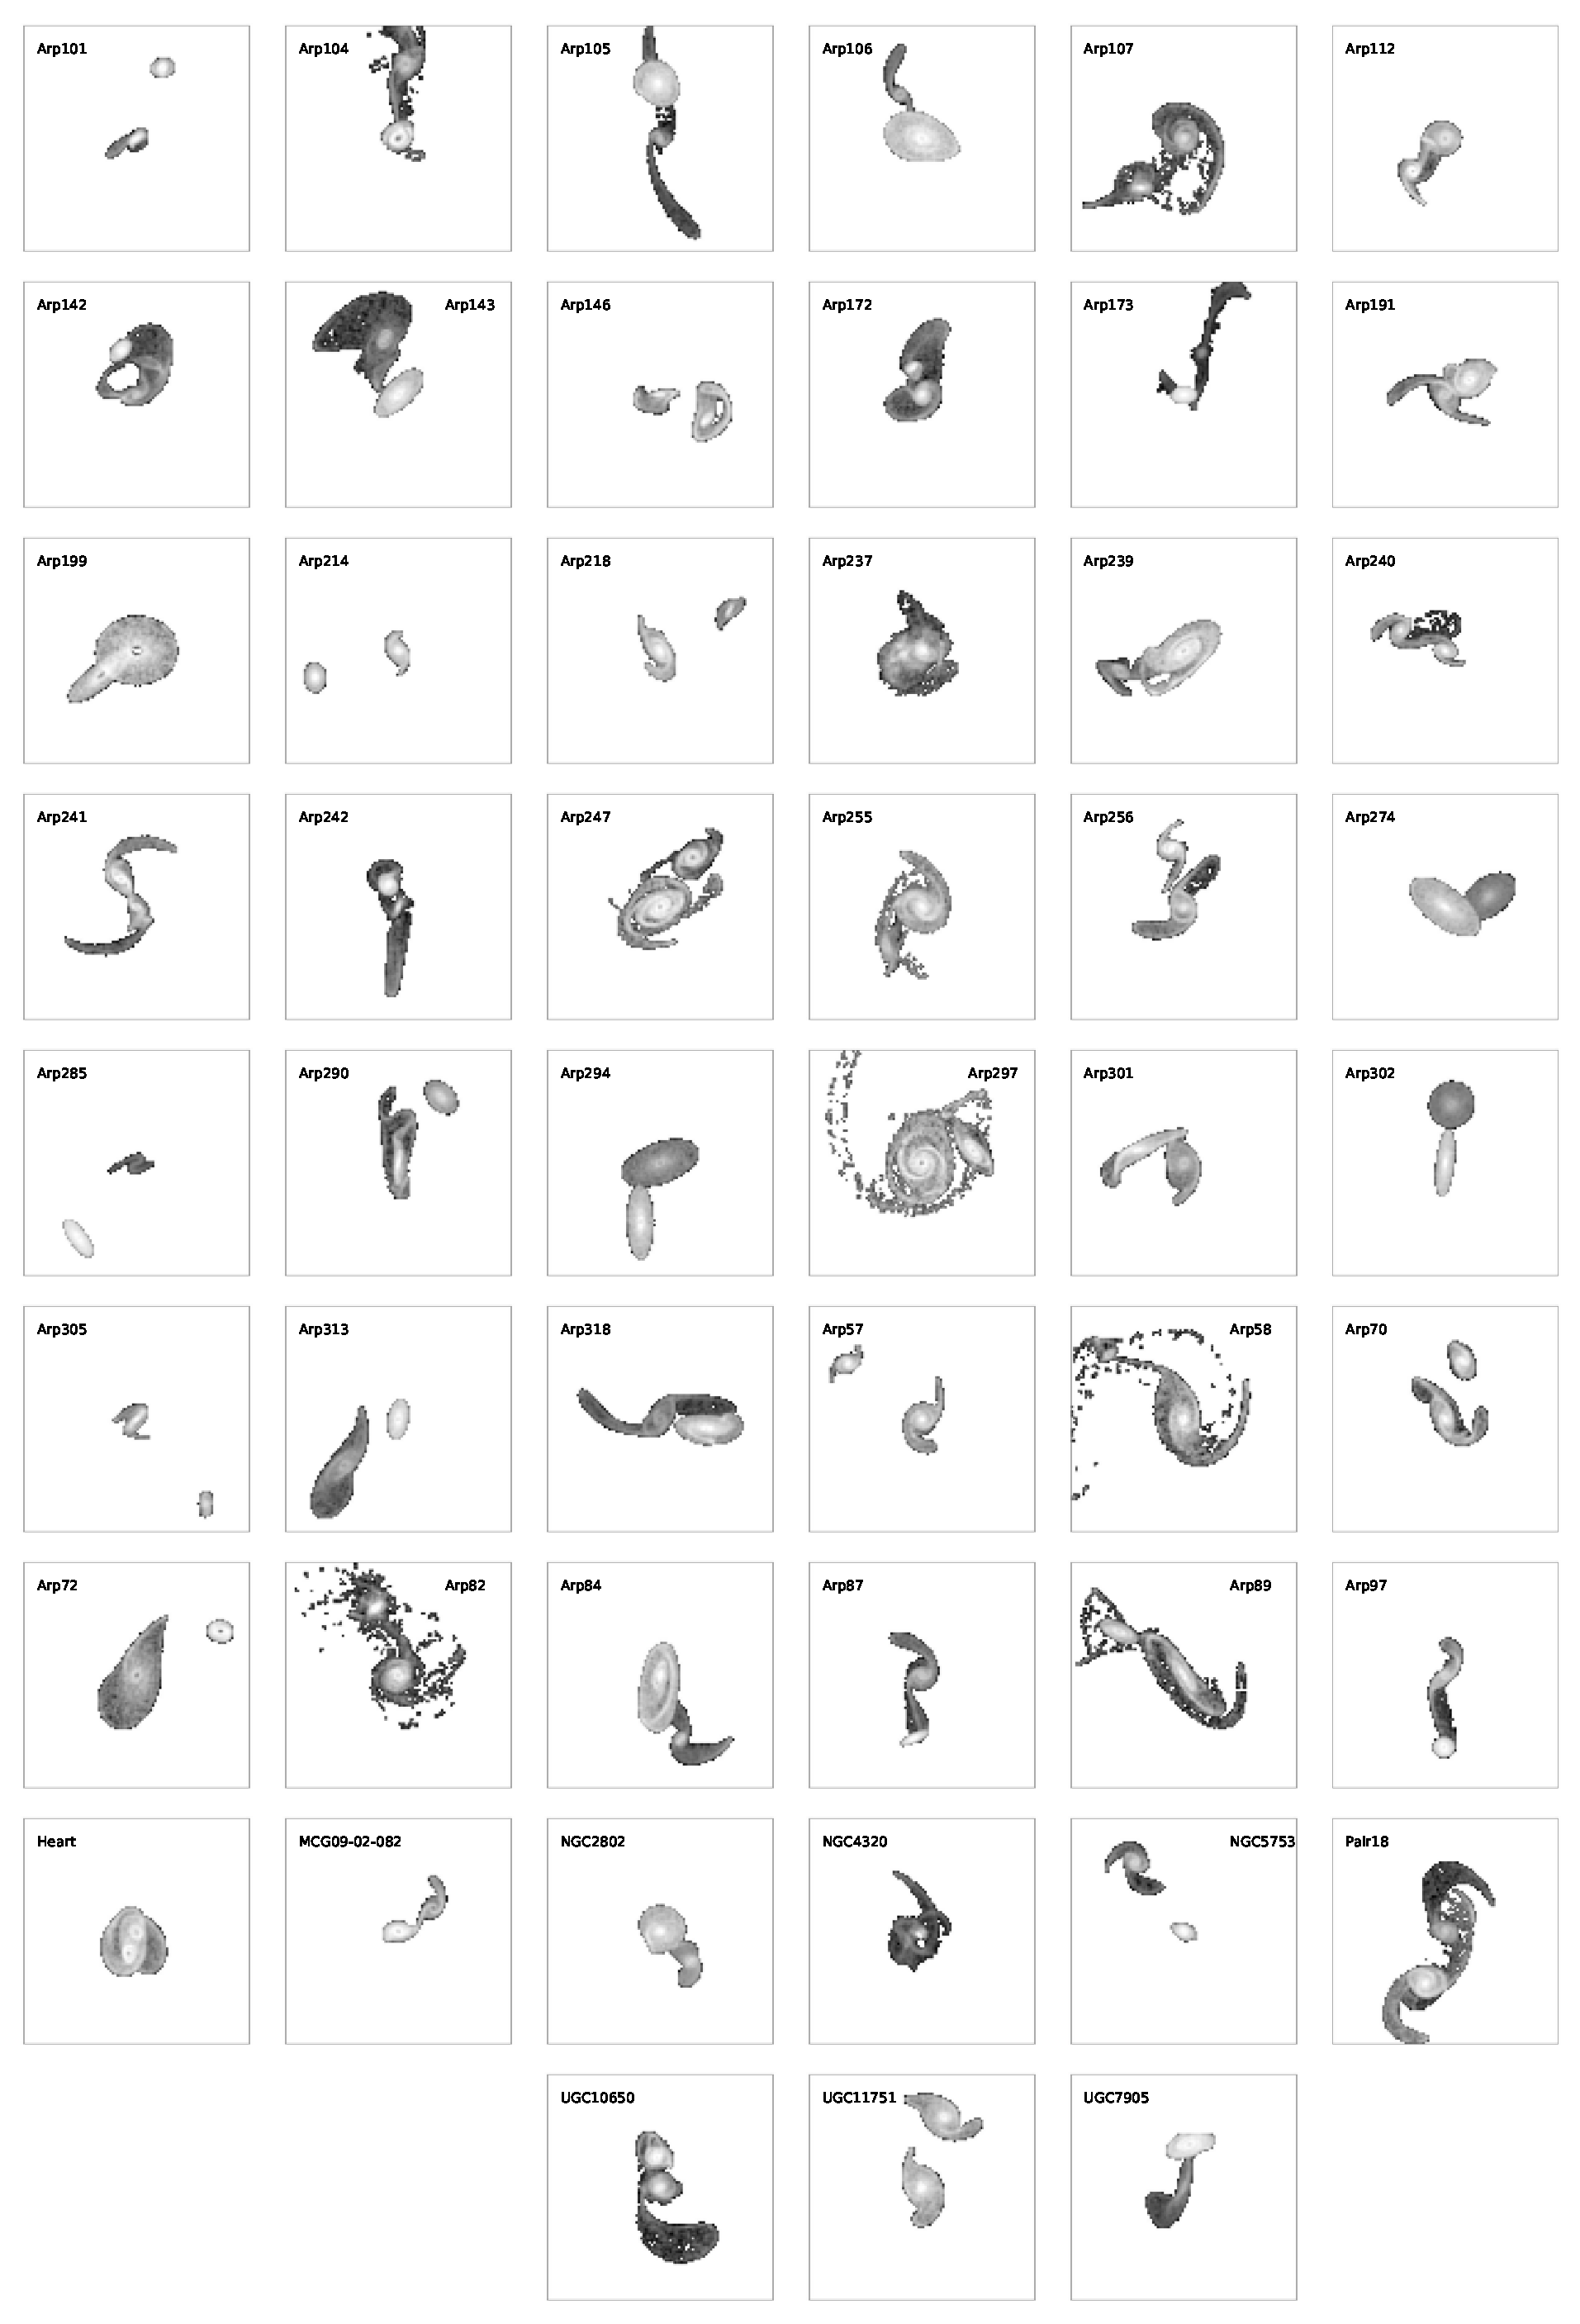
\includegraphics[width=0.90\textwidth]{Chapter1/figures/mock-images.pdf}
    \caption[Our mock observations of each interacting system.]{Our mock observations of each interacting system. These act as an idealised observation, which is completely noiseless. We also know the underlying parameters which formed these outputs. Therefore, this forms an excellent test-set to see if we can recover the underlying parameters when searching over a large parameter space.}
    \label{fig:Obj_Cutout}
\end{figure*}

\section{Constraining Interaction}\label{method:constraint}
We now require a method to compare our simulation images to our synthetic images. This comparison acts as a way to map the set of underlying parameters to an output morphology that we can then constrain by comparing to observations. However, we need a framework to conduct this comparison and to explore the parameter space of our interactions. To do this, we use an Markov-Chain Monte Carlo (MCMC) algorithm. In this section, we first describe the parameter space we explore, followed by our MCMC algorithm, how we quantify the similarity between simulation and synthetic images and how we find the parameters which are best fit.

\subsection{The Parameter Space of Interaction}
We aim to explore the underlying parameter space of interaction and find the best fit parameters which describe an input observation or test image. The parameters we constrain are the required parameters in the APySPAM three-body simulation algorithm. To function, APySPAM requires 15 different parameters. These are: the 6 positional and velocity vectors of the secondary galaxy, the total masses of both galaxies, their radius, 4 orientation parameters and the dynamical timeframe to model. We now also require the redshift measurement of the system to correctly estimate the flux distribution of the system. However, some of these parameters we can find before we begin exploring the underlying parameter space.

The first two parameters we find are the projected 2D position of the secondary from the primary. These are measured from the observational image of the system by converting between pixel and physical coordinates in the image. We take this position as the centre of the secondary disk. We also provide the redshift of the interacting system. The redshift not only directly impacts the flux distribution of the input image, but its scale and resolution. Therefore, we assume that this parameter is known and provided. Work is currently being conducted to making this a free parameter that can also be constrained based on the interacting systems flux distribution and size.

Thus, there are 13 different free parameters to recreate an interacting systems morphology and are the 13 parameters we will constrain over. A description of these parameters and the size of the parameter space explored are shown Table \ref{tab:parameters}. We choose the limits of the parameter space based on the maximum values of the parameters we used to build our test images in Table \ref{tab:Objects}. Table \ref{tab:parameters} provides the size of the parameter space as well as the conversion between the simulation units and physical units. This is primarily for reference for those who would wish to use our simulation to their own datasets. The conversions are found from \citet{1990AJ....100.1477W}.

\begin{table*}
    \centering
    \resizebox{1.00\textwidth}{!}{\begin{tabular}{|c|c|c|c|}
        \hline
        Parameter & Description & Conversion(Spec. Units) & Parameter Range(Spec. Units)  \\
        \hline
        $z$-position & Secondary $z$-position & 15kpc & -300kpc - 300kpc \\
        v$_{x}$,v$_{y}$,v$_{z}$ & Secondary velocities & 169.34kms$^{1}$ & -1693kms$^{-1}$ - 1693kms$^{-1}$ \\
        M$_{1}$,M$_{2}$ & Total Masses of Galaxy & 10$^{11}$M$_{\odot}$ & 1 $\times$ 10$^{9}$M$_{\odot}$ - 4 $\times$ 10$^{12}$M$_{\odot}$ \\
        R$_{1}$,R$_{2}$ & Radii of Galaxies & 15kpc & 0.15kpc - 150kpc\\
        $\phi_{1}$, $\phi_{2}$ & Y-axis orientation & deg & 0$^{\circ}$ - 360$^{\circ}$ \\
        $\theta_{1}$, $\theta_{2}$ & Z-axis orientation & deg & 0$^{\circ}$ - 360$^{\circ}$ \\
        t & Time of Min. Separation & 57.7Myr & 0Myr - 500Myr \\
        \hline
    \end{tabular}}
    \caption{The thirteen parameters used in both JSPAM and APySPAM to recreate an interaction. Each of these parameters must be found to consider an interaction constrained. The Parameter column shows how each parameter will be described throughout the rest of this paper. The third column then gives the conversion required to go from simulation units to SI units.}
    \label{tab:parameters}
\end{table*}

\subsection{Defining the Likelihood Function}
\subsubsection{MCMC \& Bayes Theorem}
We define framework by which to explore our parameter space, and identify areas where the parameter set successfully represent the input image. We combine APySPAM with a MCMC methodology in order to fully explore the underlying parameter space. In an MCMC, a set of walkers are created and are then moved through parameter space in an ensemble. Each walker position is a set of parameters in our 13D parameter space. At each point, we calculate the likelihood that the output simulation is representative of the input interacting system. We then compare the likelihood between the old and new position, and if the likelihood is higher at the new position the walker moves there. If not, the walker remains in place and makes another attempt to find a higher likelihood. The walkers form their own chain of steps which gradually move towards the areas of highest likelihood. In our case, the likelihood is a measurement of the similarity in flux distribution between a simulated image with parameters of the walker position and an observed image of unknown underlying parameters. Therefore, the walkers are moving from a set of underlying parameters that poorly describe the observed system to a set of underlying parameters which describe the observed system well. 

We use the well known Python package EMCEE \citep{Foreman-Mackey_13} for our MCMC. This is an ensemble MCMC package with numerous predefined moves and algorithms to make getting to the area of high likelihood more efficient. We construct contours of walker mass and use these to calculate the errors and probability distribution of our best fit measurement; i.e. we can construct a posterior for each of our parameters. For full details of EMCEE and the different modes that it can use, see the extensive readthedocs\footnote{\url{https://emcee.readthedocs.io/en/stable/}}; but here we will briefly state the hyper parameters that we use. 

For each observed image, an ensemble of six hundred walkers was initialised which would explore a total chain length of 7500 steps. Following the advice in the documentation regarding potentially complex and multi-model parameter spaces we utilised two different walker move proposals in our algorithm. These were the Differential Evolution (DE) Move \citep{Nelson_14} and the Snooker Differential Evolution (DES) Move \citep{ter_Braak_08}. An identical version of our setup can be found on GitHub\footnote{\url{https://github.com/AstroORyan}}. Here, a user can download our setup to reproduce our results, or to update the model for their own purposes.

We define a likelihood function to compare the input images to our simulation outputs. By Bayes Theorem, the probability that a set of underlying parameters which produced a simulation also describe a test image follows Equation \ref{bayes},
\begin{equation}\label{bayes}
    P(H_{i}|D_{obs},C) = P(H_{i}|C)\frac{P(D_{obs}|H_{i},C)}{P(D_{obs}|C)}).
\end{equation}
P(H$_{i}$|D$_{obs}$,C) is the probability that some hypothesised set of underlying parameters, H$_{i}$, successfully describes some observational data, D$_{obs}$, under some prior constraints, C. Applying this to our hypothesis, H$_{i}$, allows us to utilise the prior knowledge that we have about the interacting system in question and can be used to put constraints on the parameter spaces we explore to shorten computation time. This is described by the expression P(H$_{i}$|C). This is multiplied by the likelihood that the observation is defined by the hypothesised parameters given the constrains,P(D$_{obs}$|$H_{i}$,C), all divided by a normalisation constant, P(D$_{obs}$|C).

\subsubsection{Simplifying the Prior}
In order to simplify this expression, we make assumptions about the underlying parameter space to increase efficiency and simply our computations. We first assume uniform priors for each of our 13 parameters. Therefore, we define a range of parameter values that if a walker moves outwith, we set the probability immediately to zero. The ranges we allow for each parameter are specified in Table \ref{tab:parameters}. These ranges can be tweaked, or a different prior function defined, by the user. Here, we elect to set the priors part of Equation \ref{bayes} to one.

We improve efficiency in our code further by adding to the prior based on the likelihood that tidal features will form in any given interaction. This is defined by a filter parameter, $\gamma$, and is fully described in \citet[][where it is called $\beta$ but we call it $\gamma$ here to not be confused with our star formation enhancement parameter of Equation \ref{enhancement_param}]{2016MNRAS.459..720H}:
\begin{equation}\label{gamma_param}
    \gamma_{min} = \frac{M_{1} + M_{2}}{r_{min}^{2}V_{r_{min}}}.
\end{equation}
Here, $r_{min}$ is the closest approach distance, $V_{r_{min}}$ is the relative velocity at the time of closest approach and $M_{1}$ and $M_{2}$ are the primary and secondary masses, respectively. This parameter is designed to capture two important quantities: the mutual gravitational attraction and the inverse of the closest approach velocity. Each of which is important for the resultant gravitational distortion of the interacting system. By maximising the total mass of the system, while minimising the distance of closest approach and maximising the time of closest approach (i.e. minimising $V_{r_{min}}$) we would expect stronger tidal distortion. 

In our case, we use it to inform our prior as the MCMC continues. This significantly enhances the computational efficiency and pushes the walker ensemble to areas of high likelihood quickly. In each step of the MCMC, running the simulation itself is the highest computational cost, so we calculate $\gamma$ first and then make a decision on whether to run the simulation. This decision is based on an exponentially declining probability dependent on the value of $\gamma$. This probability, or prior, is defined as 
\begin{equation}\label{tidal_prob}
    C = 
    \begin{cases}
        \exp(0.5\frac{\gamma}{\gamma_{min}}), & \text{if } \gamma < 0.5 \\
        0, & \text{if } \gamma \geq 0.5
    \end{cases}
\end{equation}
Here, $\gamma$ is a user defined cutoff, 0.5 in our case. Taking the log of this, we can directly add it to prior. If the prior is initially calculated above 100, we do not run the simulation and move the walker to a new set of parameters.

\subsubsection{Simplifying the Likelihood Function}
To further simplify the likelihood function, we can assume our probability distribution is Gaussian. This is a reasonable assumption to make as a starting point for our constraining attempts. However, as will be described in section \ref{Results} this is found to not always hold true; particularly for the orientations of the system. However, making this assumption allows us to utilise the following Equation to compare our mock observations to our observed data;
\begin{equation}\label{like_gauss}
    P(D_{obs}|H_{i},C) = (2\pi\sigma^{2}_{j})\exp(-\frac{1}{2\sigma^{2}}\sum_{j=1}^{n}(x_{j}-\mu)^{2}) \times C.
\end{equation}
Here $\sigma_{j}$ is the uncertainty in the observed image, $x_{j}$ is our mock observation and $\mu$ is the observed image. The above expression can be simplified further by noting that the expression in the exponential function is just a half of the $\chi^{2}$ difference between the observational image and the mock observational image. This is the same $\chi^{2}$ function that is used in the code GALFIT \citep{2002AJ....124..266P}. Where $\chi^{2}$ is given by;
\begin{equation}\label{chi_squared}
    \chi^{2} = \frac{1}{N - n_{dof}}\sum_{0}^{N_{x}}\sum_{0}^{N_{y}}\frac{(p_{x,y} - q_{x,y})^{2}}{\sigma_{x,y}^{2}}.
\end{equation}
Here, N is the number of pixels in the observed image, which has the number of degrees of freedom subtracted from it, n$_{dof}$. $p_{x,y}$ and $q_{x,y}$ are the flux values of the (xth, yth) pixel in the observed and simulated images respectively. $\sigma_{x,y}$ is the $\sigma$ value of the (xth,yth) pixel; this is the uncertainty in the observed images pixel value and follows the $\sigma_{x,y}$-image definition from GALFIT \citep{2002AJ....124..266P,2010AJ....139.2097P}. This is then summed over all pixels in the image, giving us a single $\chi^{2}$ value between each simulated image and observed image.

Finally, to help computation time the log is taken of our likelihood function. This leaves us with a final expression that a given set of parameters describing a simulation image also describe the observed image input into the algorithm,
\begin{equation}\label{likelihood}
    \log_{10}(P(H_{i}|D_{obs},C)) = \log_{10}(L) = - \frac{\chi^{2}}{2} + \log_{10}(C).
\end{equation}
This is used at every step of our MCMC chain, with a simulation have to be run for each.

Thus, we now have a method by which to quickly predict the resultant morphology and flux distribution that the user would observe in a set of given filters. We also have a means of exploring the likely parameter space of an interaction, given an existing observation. To test this methodology, we first apply it to an idealised scenario where we know the true underlying parameters that formed the system.


\section{Results \& Discussion}\label{Results}
\noindent We now apply our MCMC algorithm to our set of synthetic interacting galaxy images. To reduce the number of repetitive figures in this paper, we focus here on a specific system as a representative sample, and publish the results of all samples online. They are presented online\footnote{All results are found here: \href{https://drive.google.com/drive/folders/1hlFhrdoZ50JaEWWYoy0RZ3J4LSoRjmsq?usp=sharing}{Link}}. As these input images are created from APySPAM, they provide us with a set of synthetic images of interacting pairs with no noise and where the underlying parameters are known. Initially, we explore the results of running this on the synthetic image of Arp 240. We discuss how the constraints could be improved, and discuss improvements on our constraints with extra, 3D information. We then plot the results for the entire dataset, and discuss trends we see in the parameters we recover.

We apply our methodology to a set of real, observed images of interacting galaxies. We select the five which are at different stages and various levels of constraint from our test dataset. We apply our MCMC to only a subset as the computational expense is significantly increased to make constraints on the observational systems and for our MCMC to reach convergence. We compare our found best fit values with those of our synthetic system, and discuss the difference between applying this to best fit simulations and observations. Finally, we describe the applicability of our approach to other systems; keeping an emphasis on those in the low surface brightness regime and the limitations this would introduce.

\subsection{Testing on a Synthetic Image}
We apply our MCMC to a single image from our mock dataset described in Section \ref{sec:syn_sample}. We elect to use this system as it is is composed of two clear and distinct disks, with a tidal bridge connecting them and tidal tails forming on the opposite side. The tidal features lie in the high surface brightness regime, and have an inclination close to 0. The observation and synthetic image are shown in Figure \ref{fig:arp240}. There are clear differences between the morphology of our mock image and the observation of Arp 240. Therefore, testing on the synthetic image is not the same as constraining the Arp 240 system. However, the synthetic image is an ideal scenario to test our methodology on. We elect to test our MCMC on the Arp 240 system first, as it has a high mass in our sample meaning the tidal features will contain more flux and should be easier for our MCMC to constrain.

\begin{figure*}
    \centering
    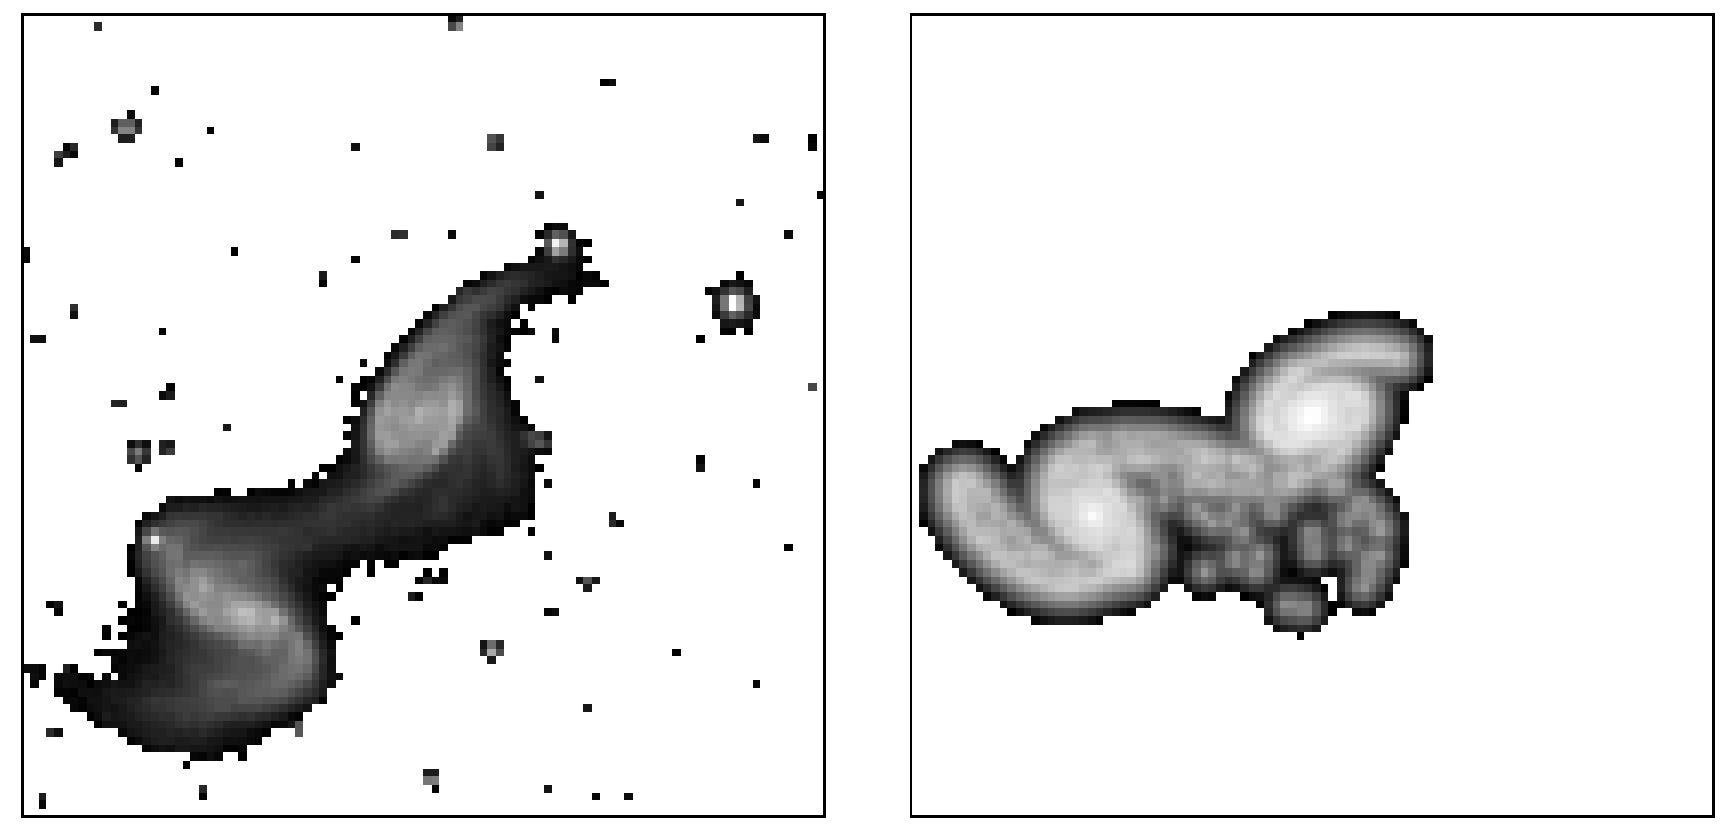
\includegraphics[width=0.75\textwidth]{Chapter1/figures/arp240-obs-sim.pdf}
    \caption[The example system used to test our MCMC: the Arp 240 interacting system.]{The example system used to test our MCMC: the Arp 240 interacting system. This system is considered an easy one to constrain. It is composed of two clearly distinct galaxies, with strong tidal features that our MCMC can match. These tidal features are the two tidal tails formed in the interaction and the tidal bridge linking the two systems. \textit{Left}: The prepared observation image of the Arp 240 system created from SDSS DR16 observations. \textit{Right}: The best fit simulation image as found by \citet{2016MNRAS.459..720H} and the first test image used in our pipeline. The different in scale and orientation are discussed below.}
    \label{fig:arp240}
\end{figure*}

We constrain the synthetic Arp 240 image by running our simulation with 2,500 particles with 600 walkers and 7,500 steps in the MCMC. An example of our full results is shown in Figure \ref{fig:corner_plot}. This corner plot is created using the Corner Python Package \citep{corner}. However, displaying our results as is shown in Figure \ref{fig:corner_plot} will be difficult as we will be discussing multiple different systems throughout this section. This larger corner plot also uses a lot of space. Therefore, we will present and discuss our results using reduced corner plots as shown in Figure \ref{fig:arp240_corner_plot}.

\begin{figure*}
    \centering
    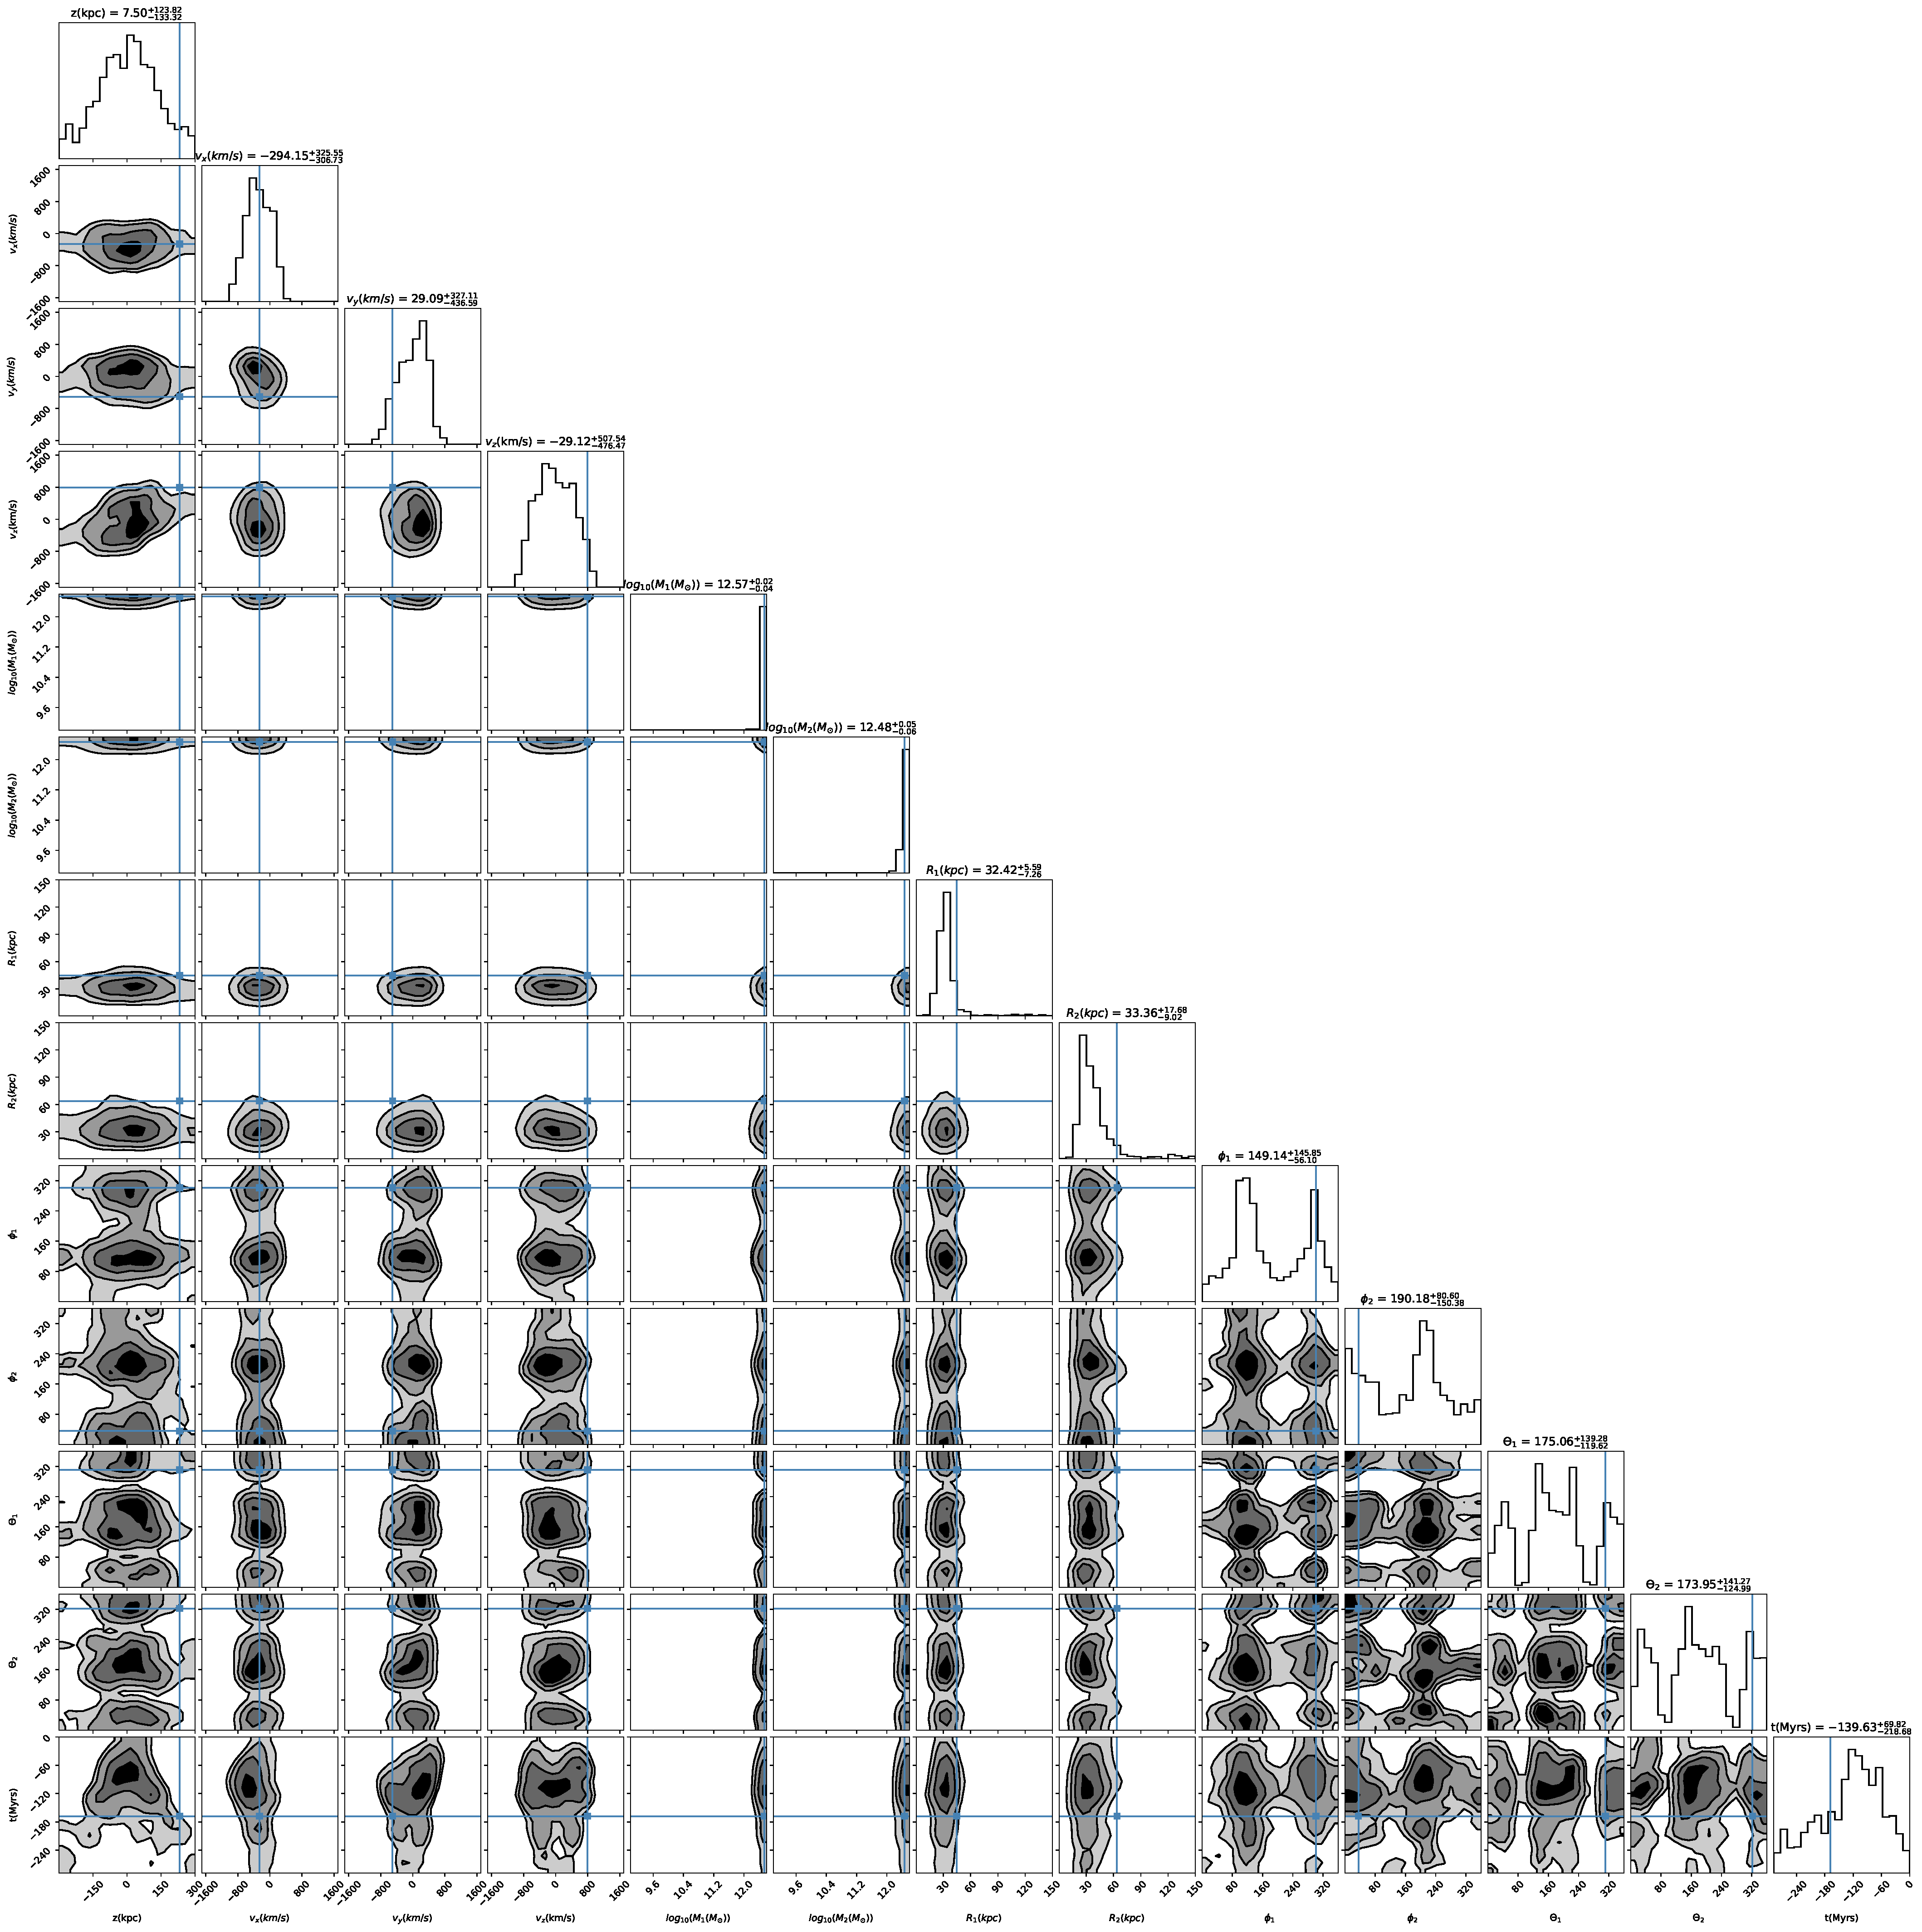
\includegraphics[width=\textwidth]{Chapter1/figures/Arp240-full-corner.pdf}
    \caption[Corner plot showing the constraints made on all thirteen parameters we are exploring.]{Corner plot showing the constraints made on all thirteen parameters we are exploring. Each contour level contains 11.8\%, 39.3\%, 67.5\% and 86.4\% of the samples across all walker chains. Displaying our results using the full corner plot is difficult in a paper because of the high dimensional results that we obtain. Therefore, we elect to show all remaining results in this paper as reduced corner plots like Figure \ref{fig:arp240_corner_plot}. We elect to put the parameters which are most likely to correlate together in different corner plots. To view the full corner plots of each system, find them at the results website for this paper.}
    \label{fig:corner_plot}
\end{figure*}

\begin{figure*}
    \centering
    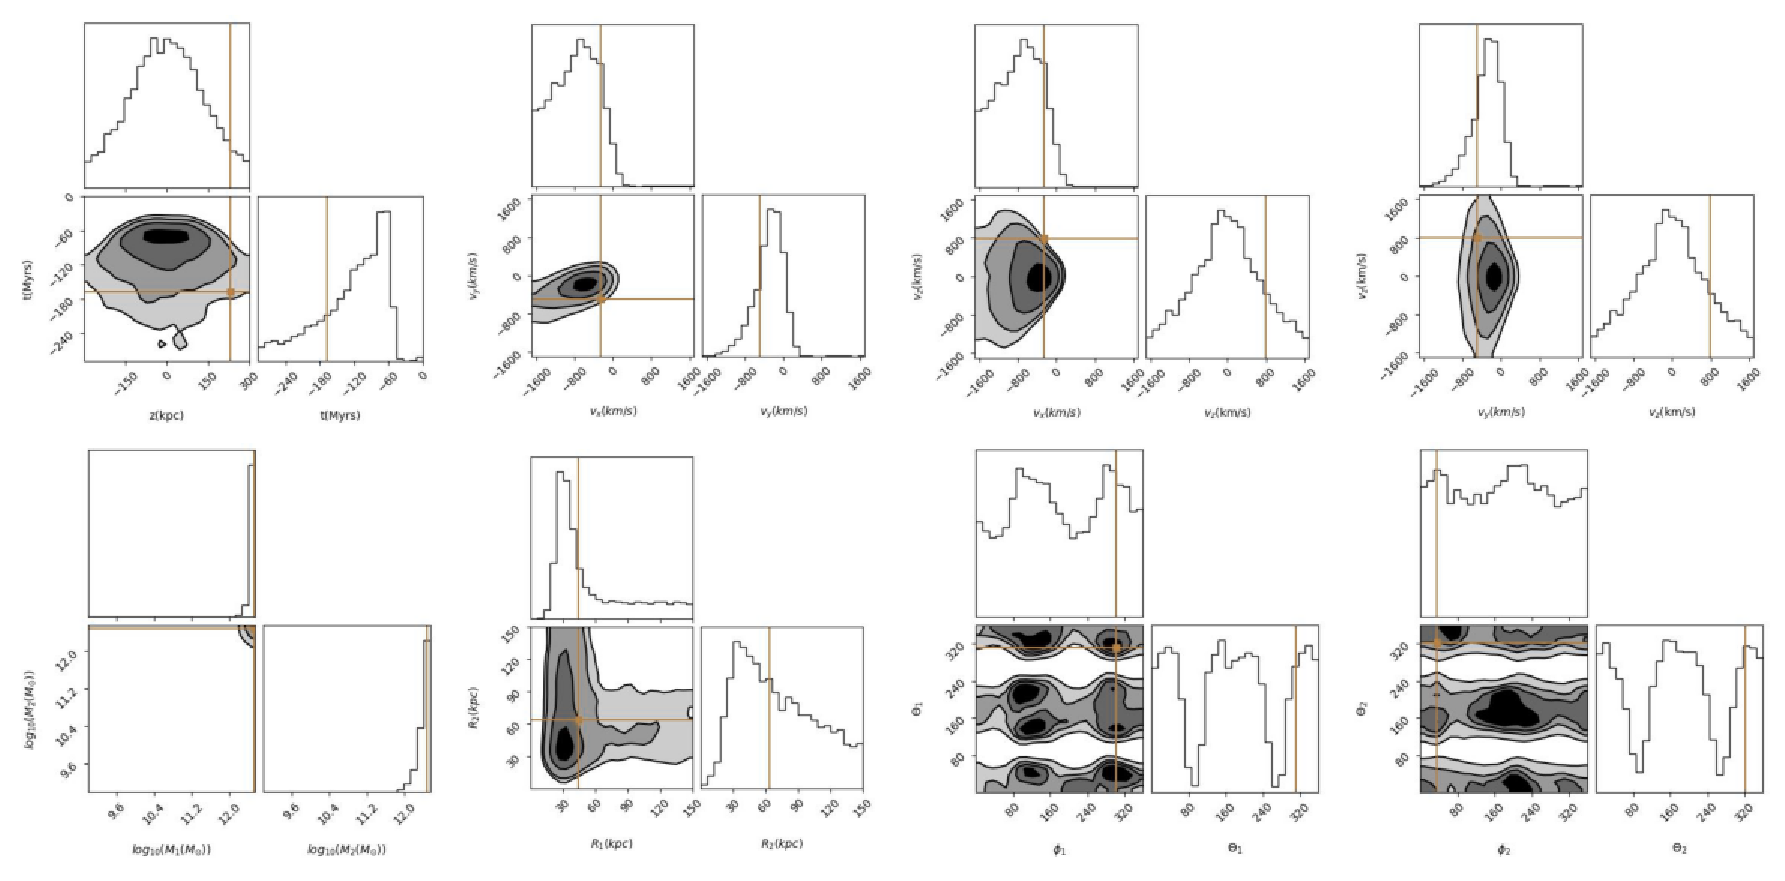
\includegraphics[width=\textwidth]{Chapter1/figures/Arp240-red-corner.pdf}
    \caption[Same as Figure \ref{fig:corner_plot}, but reduced to only corresponding parameters.]{Same as Figure \ref{fig:corner_plot}, but reduced to only corresponding parameters.}
    \label{fig:arp240_corner_plot}
\end{figure*}

% Describe the results, what are we looking at?
Figure \ref{fig:arp240_corner_plot} shows the constraints we have found on each parameter from our MCMC. The golden lines then show the true values used to create the synthetic image, and are those described in Table \ref{tab:Objects} for Arp 240. The contour levels correspond to 11.8\%, 39.3\%, 67.5\% and 86.4\% of the samples across all walker chains (these are default values), indicating the confidence level (CI). For reference, we have set up the corner plots here such that the contours containing 68\% of the walkers roughly corresponds to 1$\sigma$\footnote{Full explanation in Corner plot Docs: \url{https://corner.readthedocs.io/en/latest/pages/sigmas/}}. However, this assumes a Gaussian probability distribution, which is not strictly true for the results we find here. Figure \ref{fig:arp240_corner_plot} shows that each of the truth values is within a 67.5\% CI of the probability distribution with the exception of the $z$-position and time.

% Why do the results look like this?
We get excellent constraints on the masses of the two galaxies. This system is the most massive system in our sample, and therefore we expect the mass at the very limits of the range we are exploring. We find that the MCMC first converges on the two masses of the disks, and are the easiest for us to constrain. We provide the algorithm with the secondary 2D position, and therefore it only has to fit the flux distribution of the inner disk correctly to get good constraints on the galactic masses. The largest gains in likelihood maximisation come from matching the flux distribution in the inner parts of the primary and secondary. While the formation of the tidal features depends on the mass ratio, they also depend heavily on the orientation of the interaction as well as the relative sizes.

The relative sizes of the disks is important for the constraining the tidal features as it is the outer parts of the disk that are sheared off to form them. The primary radius is constrained very well, and is primarily expected to be smaller than the true value of this system. This is, again, due to the $\chi^{2}$ nature of calculating the distance between the two images. The likelihood, on average, is lower with some pixels within the galaxy being missed than a pixel containing the central disk in it when it should not. We therefore have a bias effect where the peak of probability drifts to just below the true value of the radius. However, the true value of the radius remains within 86.4\% CI of the found contours. 

The recovery of the radius of the secondary is worse than that of the primary. We find the peak in the probability distribution is far lower than the true value. This is from a limitation of our simulation as well. While the output simulations of the MCMC are always centred on the primary, the secondary galaxy central position is not so certain. Due to the backwards integration and trajectory calculated here, the secondary does not always end in the exact same image bin in the output simulation image. Therefore, the secondary disk likely moves slightly per simulation. This change transfers further uncertainty in the secondary disk size, and a preference for the secondary to be smaller to improve the likelihood calculation. The size of the secondary disk also contributes much more to the tidal debris formed in the interaction. The simulation is conducted in the frame of the primary, leading to the 3D velocity of the secondary being higher than that of the primary. Therefore, the particles in the secondary are much more likely to be ejected during the encounter than the simply orbiting primary particles. This adds further uncertainty to the secondary radius. However, once again, the best fit values found are within 84.6\% CI of the true value from the base simulation. 

There will also be some uncertainty involved in this measurement from the formation of the tidal features. The flux distribution of the tidal features that form are inter-dependent on multiple parameters; primarily the mass ratio, the size ratio and the orientation of the galaxies in the interaction. The significant degeneracy in the orientation constraints undoubtedly has some effect on the fitness of the resultant system. Due to a lack of three dimensional information, our algorithm cannot discern which way the galaxy is rotating or which way the tidal features should be orientated in the line-of-sight. Therefore, degeneracy at $\pm180^{\circ}$ of the true parameter values for $\phi$ and $\pm$180$^{\circ}$ for $\theta$. Figure \ref{fig:arp240_corner_plot} shows this with several different peaks in both measurements of $\phi$ and $\theta$. However, we recover the true parameters in one of the peaks of the marginalised posterior for each orientation parameter.

It is important reiterate here that $\phi$ is the orientation of the galactic disk with respect to the $y$-plane while $\theta$ is the orientation with respect to the $z$-plane. With 3-dimensional information, such as the direction of rotation of the disks or the line of sight (LOS) velocities of the tidal features, we would be able to resolve the degeneracy in the $\phi$ parameter. However, The source of the degeneracy in $\theta$ has a different source. The tidal features can form in the opposite direction from the mock observation and still be found to have high likelihood. This is a result of our likelihood being based on flux matching on pixels. There is no knowledge provided of the direction the tidal features should be moving or forming, only if the pixels contain the correct flux. Therefore, this gives a significant degeneracy in the $\theta$ parameter. Therefore, while the disk can be flipped in the $z$-direction and still match the observation, it can also be flipped in the $y$-direction as well. While the degeneracy in $\phi$ can be solved with velocity information, the $\theta$ orientation will require information on the rotation of the disk itself. Having rotational information will allow us to constrain the bulk motion within the galaxy and the direction the inner disk should be rotating as well. These two pieces of 3D information will remove the 4-fold degeneracy in each parameter.

The lack of 3D information also affects our constraints in the z-direction: the $z$-position and the $z$-velocity. As seen in Figure \ref{fig:arp240_corner_plot}, the finds the peak in the posterior distribution for both parameters as much lower than they truly are. First, the $z$-position is difficult to constrain as we lack 3D information. The simulation is run in the reference plane of the primary galaxy, therefore the secondary can only be behind or in front of iy. There will be change in the flux of the secondary based on whether it is in front or behind of the primary galaxy. However, this change in flux is completely dominated by the distance due to the redshift of the galaxy. Therefore, there is little to no observable change in the absolute values of flux unless the true value of the $z$-position was very large.

The constraint of the $z$-velocity remains far from the true parameters due to similar reasons as above. The true value lies at the very edge of the probability distribution found, at approximately 86.4\%. This would, again, be rectified readily by introducing velocity information into our constraints. The simulation works so that the secondary galaxy is always at the same x and y position that is defined by the user. Therefore, an output simulation with a positive or negative LOS velocity will have the same flux distribution. Hence, this constraint simply peaks about zero for the $z$-velocity.

Our MCMC works significantly better, however, with the $x$- and $y$-velocity of the secondary galaxy. We find the the truth value of this is within 67.8\% CI of our found distribution. The velocity values are directly related to the strength of the interaction, and therefore indirectly relate to the tidal features which form. Thus, our MCMC is informed by the flux distribution of the resultant simulated image and gives an excellent constraint on the parameters.

% Need to replace this time of interaction with the correct one. 
Finally, we discuss attempting to constrain the time of the interaction. We show the time since closest approach, not the total interaction time. The underlying simulation utilises backwards integration to calculate the trajectory of the interaction. Therefore, the time we input into the simulation simply tells it how far back in said trajectory to put the secondary galaxy. Therefore, the same interaction will occur whether we input -10 time units or -100 time units. The algorithm will require more computation time to calculate the particle positions in the lead up to the interaction. It is important to note that the total integration time will only affect the output system when we make it too small. In other words, if the secondary starts after the point of closest separation or at closest separation, our simulation breaks down and gives nonphysical results.

We calculate the time of closest approach for all of our walker steps and then present this as a measure of the time posterior distribution. Our measured value is significantly smaller than the true value of our best fit simulation, although it does lie within the region of 86.4\% CI. This parameter is highly dependent on the velocity and position constraints that we have made, and these are skewed to significantly smaller values than the truth. Therefore, it is unsurprising that our time of closest approach value is also found to be much smaller.

To fully put this result into context, we explore the simulations that lie in the areas of highest probability within these posteriors. To select which simulations to present, we take those walkers that were within the 11.8\% CI throughout each walker chain and take the top 5 as an illustration here. Our MCMC is not able to precisely reproduce the input image. It is often able to reproduce the tidal features of the primary as well as the tidal bridge connecting the two systems. This appears to be where the MCMC has centered the posterior upon. The likely reason for this is actually due to the filtering parameter that we use on the simulation. The Arp 240 simulation lies in an unlikely area of tidal features to form - $\gamma = 0.259$ - and, therefore, we update our prior to make the true result appear less likely. However, the $\gamma$ parameter remains a necessity in our MCMC. Without the ability to filter the simulations quickly, we begin to approach very large requirements of computational expense. Therefore, for this particular example the $\gamma$ parameter is a hindrance.

\begin{figure*}
    \centering
    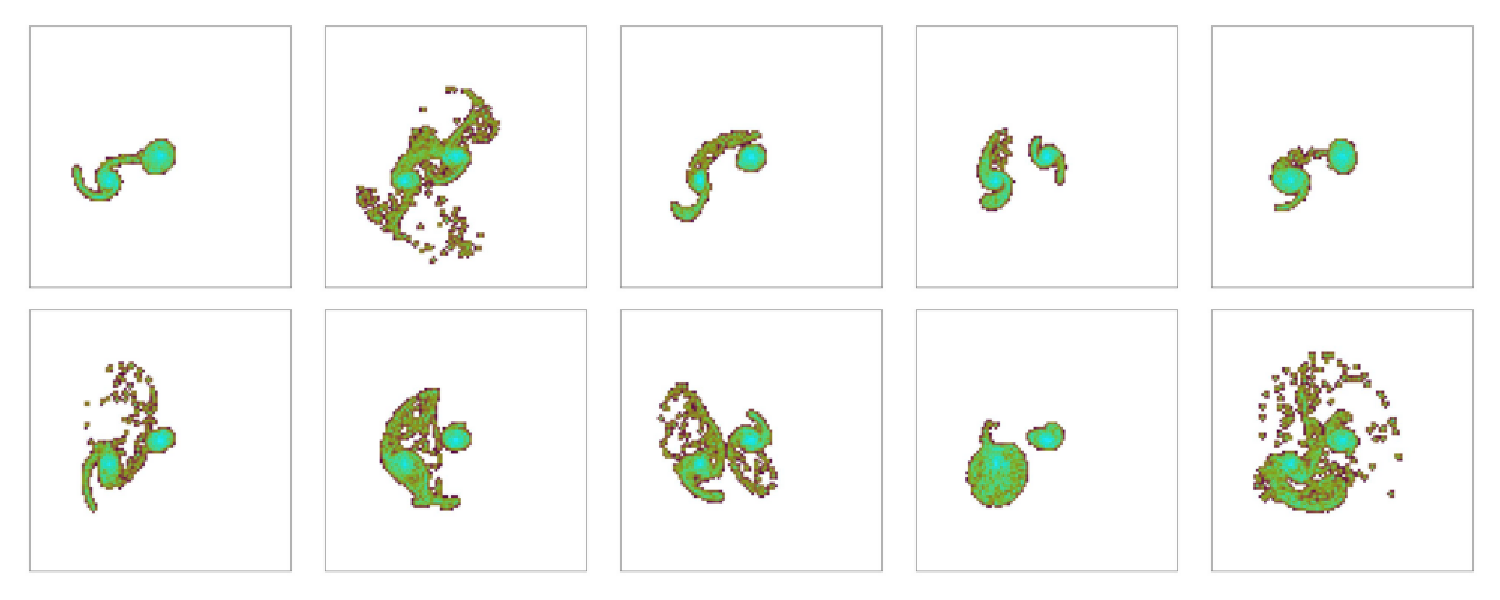
\includegraphics[width=\textwidth]{Chapter1/figures/best-fits-comb.pdf}
    \caption[Simulations from the areas of parameter space that lay within the 11.8\% CI of our constraints.]{Simulations from the areas of parameter space that lay within the 11.8\% CI of our constraints. \textit{First Row}: The synthetic image we are attempting to constrain. \textit{Second Row}: The best fit simulations from this parameter space. \textit{Bottom}: The worst fit simulations from this parameter space. Our MCMC found those parameters which cause the formation of the correct tidal features, as well as the tidal bridge connecting the two systems. However, it has been unable to fully identify the tidal features of the secondary. There is also a lot of noise in this posterior distribution, with many systems with different tidal features in the areas of high probability. Therefore, identifying specific systems with the sought after tidal features requires manual intervention.}
    \label{fig:arp240_corner_plot}
\end{figure*}

% This is likely better in the conclusion.
In the surrounding area of probability space, however, we find some interesting constraints. Changing each parameter by small amounts based on the posteriors of each parameter space leads to variation in the simulation outputs and tidal features. Due to the disks being well defined and aligned, this can often lead to them being weighted highly. Therefore, the question remains, how would one use this code to find their best fit simulation and actually make constraints using it? This algorithm is best used as an indication of where in parameter space the true parameters lie in recreating the tidal features observed in an observation. This reduces the size of parameter space to explore dramatically, and could be an indication of where to search with more accurate simulation models for true interacting galaxy parameters.

Overall, from our example of Arp 240, we are able to recover nearly all the true values of the input simulation to within an 86.4\% CI of the true parameters. The only missing parameter is the time since the flyby. There is significant degeneracy in constraining the orientations of this interaction, but this is expected. While our results appear like they have converged in the MCMC, we will also describe the diagnostics with which to prove this. 

\subsection{Diagnostics of Pipeline}
% Note, a quick section to discuss the diagnostics of the pipeline, proved it's converged etc. If I cannot get Chain Consumer working here, then I won't do this section.
\noindent It is important to ensure our results are reliable by using diagnostics to investigate the MCMC chains. We investigate three different diagnostics of our MCMC run. First, we check that they have truly converged with the Geweke diagnostic. The Geweke diagnostic is a Z-test of equality of means where the autocorrelation in the flattened samples is taken into account as the standard error is measured. We compare the means of the first 10\% and last 50\% of each chain in each parameter, and require the resultant Z-score to be $<1$ for convergence. We use the Geweke diagnostic as written in the ChainConsumer \citep{2016JOSS....1...45H} Python package. For this case, every parameter passes this convergence test, with the exception of the orientation parameters (although, this is likely the result of converging on multiple best-fit values).

Figure \ref{fig:arp240_corner_plot} clearly shows that each orientation has incredibly complex, multi-model structure in the parameter space. We have a 2- or 4-fold degeneracy in the output models due to three dimensional information not being available. This disrupts our Gewke diagnostic measure, which is looking for a single peak in parameter space. Therefore, by folding the parameter space over and only exploring over $0^{\circ}$ - $180^{\circ}$, we achieve a single peak in parameter space. These results then pass the Geweke diagnostic test.

\begin{figure}
    \centering
    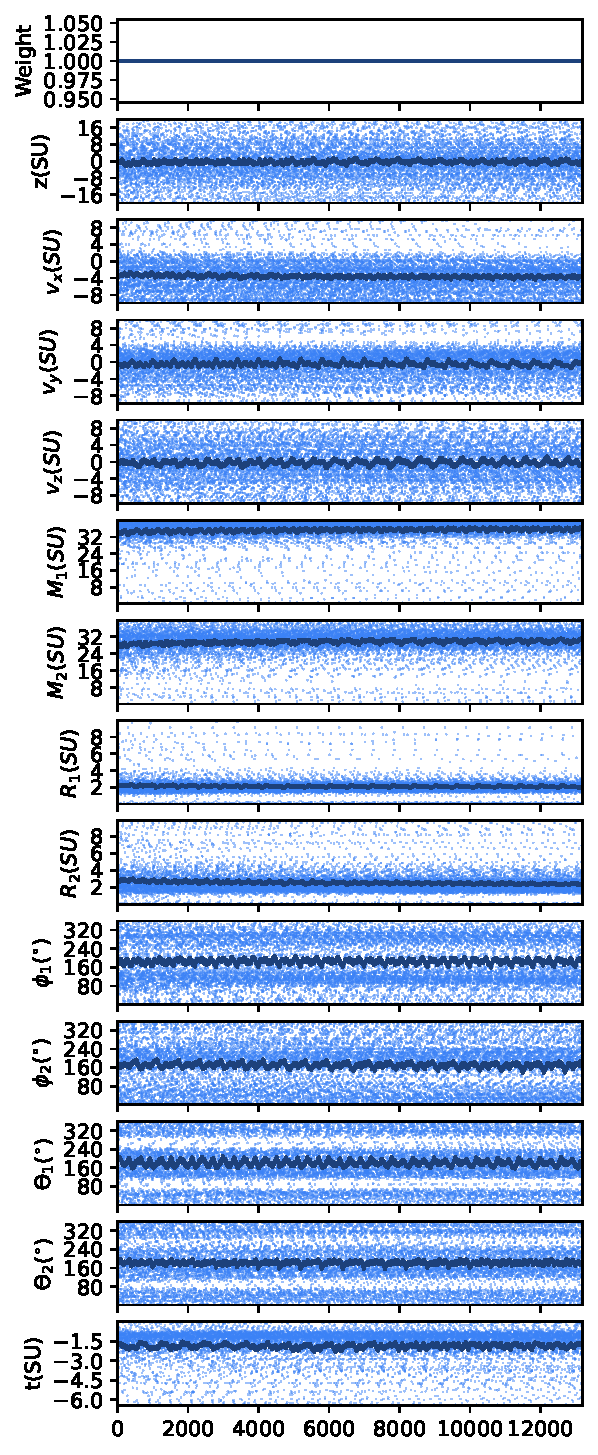
\includegraphics[width=0.45\textwidth]{Chapter1/figures/arp-240-steps.pdf}
    \caption[Steps taken by each walker in our MCMC chain to constrain the Arp 240 best fit simulation.]{Steps taken by each walker in our MCMC chain to constrain the Arp 240 best fit simulation. Note, the $y$-scales here do not extend over the full parmaeter space for some galaxies, and only show where the walkers have stepped after the burn-in phase. The deeper the blue, the more walkers have stepped at that point. This figure shows that our MCMC has successfully burnt in and very quickly goes to high areas of probability for parameter space. They then oscillate around the best fit values while searching the remaining parameter space. The $z$-position, $z$-velocity and $\phi_{2}$ parameters show dignificant uncertainty as the walkers move around the entire parameter space. In the $\phi_{1}, \theta_{1}, \theta_{2}$, we can see the two fold degeneracy form very early on and then the walkers do not explore across them at any point.}
    \label{fig:walker_steps}
\end{figure}

The second diagnostic we use is that the walkers have fully explored parameter space and that we have removed enough of the steps at the beginning of the run to consider the MCMC burnt-in. Once again, using ChainConsumer, we can plot out each walker step throughout parameter space. Figure \ref{fig:walker_steps} shows the flattened walker chains through parameter space. We have removed the first 200 steps of each walker chain before thinning the chain and flattening it. By flattening we have taken each walker chain and combined them into one chain for every parameter. Discarding the first 200 steps has been enough for the burn in of the MCMC, as the walkers have already moved mostly through parameter space and are centering on a central value of high probability. The structure in the orientation parameters is also interesting. The degeneracy structure in the parameter space has already formed by the end of the burn-in and then the walkers move within those areas of high probability. This is for two reasons. First, they affect the flux distribution of the disks primarily in if they are face-on or edge-on. The MCMC quickly converges on face-on systems in our case. Second, when they are in that degenerate space, the slight changes in inclination of the disks given does not change the likelihood calculation significantly enough to reduce this degenerate space further. Hence, the degenerate areas are very large with very flat areas of probability at their peak.

We have tested resolving this problem by running further steps in our MCMC to achieve convergence naturally within the parameter space. We find that increasing the number of steps does improve convergence on the orientation parameters, but at a much larger computational cost and without substantial improvement on the other parameters. Therefore, we elect to fold our resultant degenerate solutions into a smaller parameter space. This achieves convergence, and gives us excellent estimates on the orientation for these systems.

A second solution to this problem would be involving velocity information into our models. Knowing the bulk motion of the tidal features would allow us to constrain the tidal features based on which way they were rotating. This would eliminate part of the degenerate space. However, as stated previously, little spectroscopic data exists of our sample of interacting galaxies. Therefore, we run this test using the our synthetic Arp 240 image and including the LOS velocity of the particles and creating a velocity grid to constrain over.

\subsection{Inputting 3D Information}
Very few of the systems described in Table \ref{tab:Objects} have associated integral field spectroscopy (IFU) data in order to get LOS velocities to incorporate 3D information into our fitting process. This is because they are very large in the field-of-view of many instruments, and therefore we can only achieve measurements of their inner disks and not their tidal features. We, therefore, map the velocity distribution of our synthetic Arp 240 image. This map is created by summing the $z$-velocities of each particle in the bin and then create a total LOS velocity map for which to compare to simulations. This has little impact on the measurements of mass, size and $x$- and $y$-velocity measurements. However, it completely changes our measurements of the $z$-position and time of interaction as well as improves our constraints on all three velocity vectors dramatically. 

Figure \ref{fig:velocity_corner_plot} shows the new measurements of the constraint on the $z$-position, $y$- and $z$- velocities. The constraints on each of these parameters is significantly improved. This is with the same number of MCMC walkers and steps as without 3D information. For the $y$- and $z$-velocities, the constraints are improved to the point where we completely recover the true underlying parameter values within 39.3\% CI. With the $z$-position, we also gain significant constraint. We are able to recover which side of the primary the secondary lies, with a sharp drop in the marginalised posterior over the negative part of the $z$-position parameter space. We also significantly improve our constraint on the time of the interaction, and approximately recover the true parameter. We are able to constrain the final velocity expected in the observation, and therefore, means the galaxy cannot be moving too fast at in the final timestep. This has the effect of shifting the expected time of contact back significantly.

\begin{figure*}
    \centering
    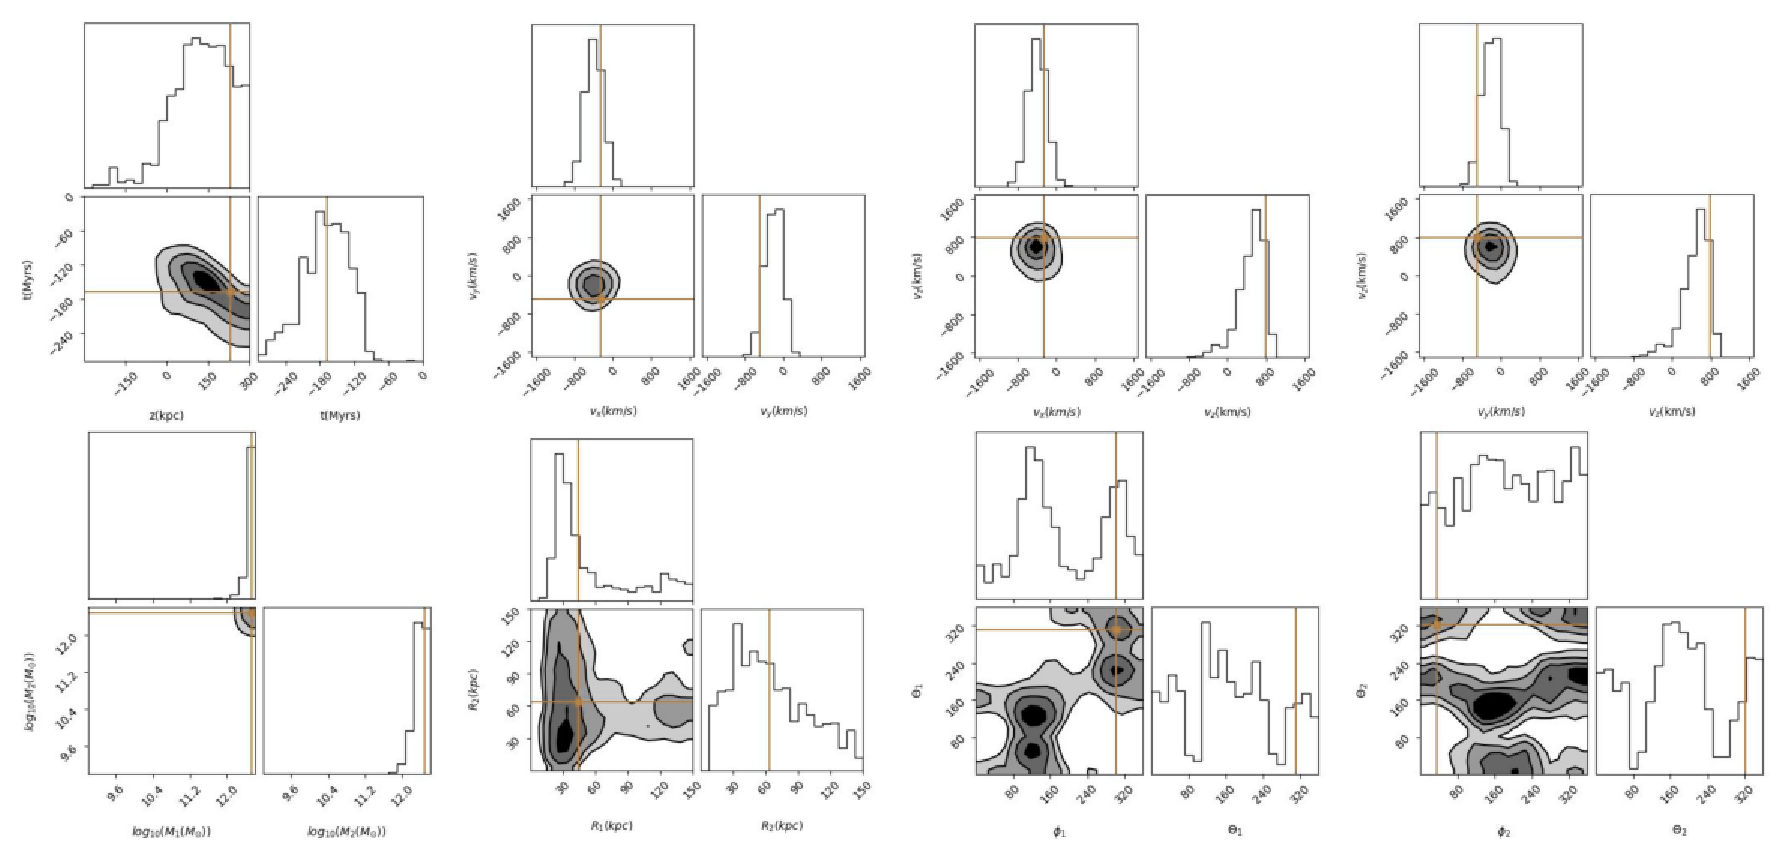
\includegraphics[width=0.9\textwidth]{Chapter1/figures/Arp240_vel-red-corner.pdf}
    \caption[The reduced corner plot of the synthetic Arp 240 system with a velocity map also used for constrained.]{The reduced corner plot of the synthetic Arp 240 system with a velocity map also used for constrained. To add this extra information, we created a mock velocity map of our Arp 240 synthetic image and summed the LOS velocity ($z$-velocity) in each pixel of our image. Comparing between here and Figure \ref{fig:arp240_corner_plot}, we see we make different constraints on the $z$-position and the time as well as resolve one of the degeneracys in the orientation space.}
    \label{fig:velocity_corner_plot}
\end{figure*}

Interestingly, we lose a significant amount of constraint on the relative sizes of the two systems. Adding the velocity information in the way we have likely increases the required size of the disks so the LOS velocities match within them. Therefore, more particles are stripped from the secondary galaxy and cause further uncertainty in the final image. We also find the removal of some of the degeneracy in the orientation parameters, as expected. It is important to note that, in this example, we have only used the LOS velocities to achieve this improvement in constraint. To better get constraint on orientation, we likely need further velocity and 3D information of the system. For instance estimates of the internal rotation, and accurate measures of the bulk motion of the tidal features in the galaxy. Currently, the simulation is not able to accurately reproduce this outwith simply assuming circular velocities at different radii from each galactic centre. Finally, the mass constraints remain the same as was found without velocity information as they are dependent primarily on the flux distribution and dominated by the inner disk of the system.


This shows the improvement that adding velocity information to our MCMC could bring, and how far interacting galaxy simulation and constraint can go once we incorporate IFU spectroscopy over more systems. In the sample we are using here, of the most massive, large, major interacting systems, only three have got any IFU data. This data is from the MaNGA \citep{2015ApJ...798....7B} IFU spectrograph, whose field of view is only able to capture the central disk of these systems. While having velocity information on even a subset of the pixels of the galaxy would improve constraints, to significantly improve them we will need this of the full tidal features of the systems. IFUs with larger fields of view are soon to come online, such as WEAVE \citep{2014SPIE.9147E..0LD}. 

\subsection{Running on Full Idealised Sample}
% Remember, this section is meant to be an overview of all of the results and simply a discussion on what we notice of applying it to different systems. This is not another deep dive like we did in the testing on one system. 
\noindent With constraints being ascertained on nearly all parameters of our synthetic Arp 240 image, we then applied our MCMC to the remaining 50 synthetic images. The reader is invited to see the resultant corner and reduced corner plots of each system on the website. Here, we will detail describe our best and worst three corner plots, and then discuss the trends throughout applying the MCMC to the dataset. First, our ability to constrain is highly dependent upon the stage of interaction. Our tightest constraints, the ones with narrowest posteriors, were on those interacting galaxies which were only just past the point of closest approach. I.e., they were the systems which had highly distinct tidal features and disks were fully separate. Our best three fits were those of synthetic images of Arp 172, Arp 240 and Arp 290. The `best fits' have been judged by those with the smallest FWHM of their marginalised probability distribution in mass. The reduced corner plots are shown in here in Figures \ref{fig:arp240_corner_plot}, \ref{fig:best-Arp172} and \ref{fig:best-Arp290}. Each of these systems is clearly in stage 2 or 3 of the interaction, where tidal features have formed clearly, and there are two distinct disks.

\begin{figure*}
    \centering
    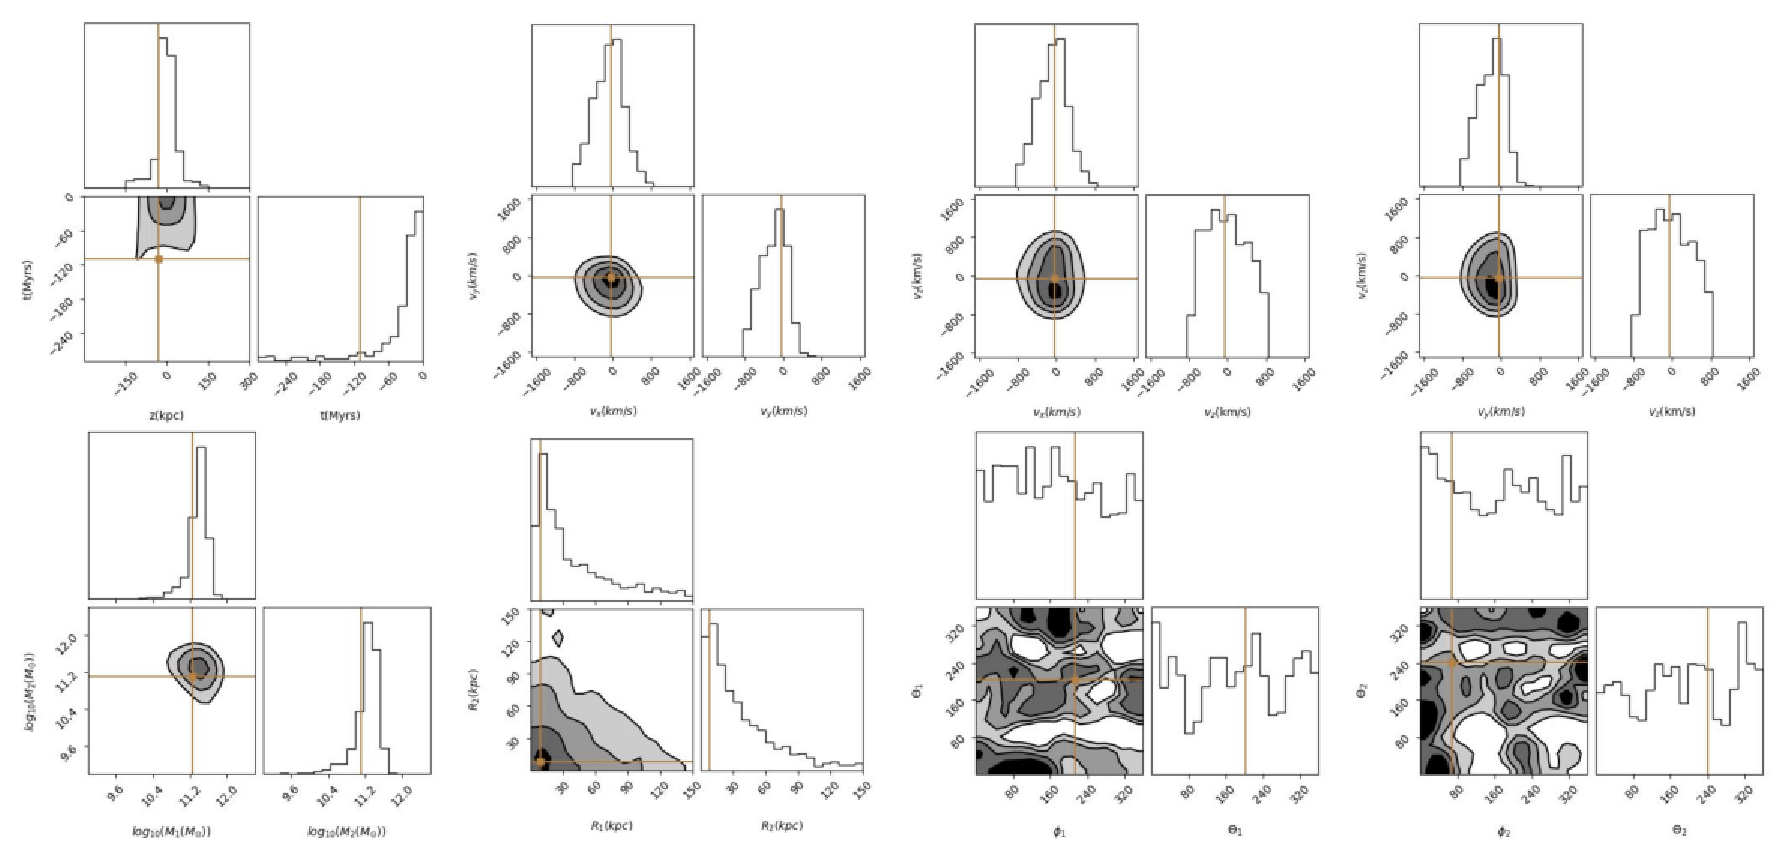
\includegraphics[width=\textwidth]{Chapter1/figures/Arp172-red-corner.pdf}
    \caption[Second example of our best fits from our methodology is representative of the simulated image of Arp 172, a stage 3 system.]{Second example of our best fits from our methodology is representative of the simulated image of Arp 172, a stage 3 system. Gold lines represent the true values.}
    \label{fig:best-Arp172}
\end{figure*}

\begin{figure*}
    \centering
    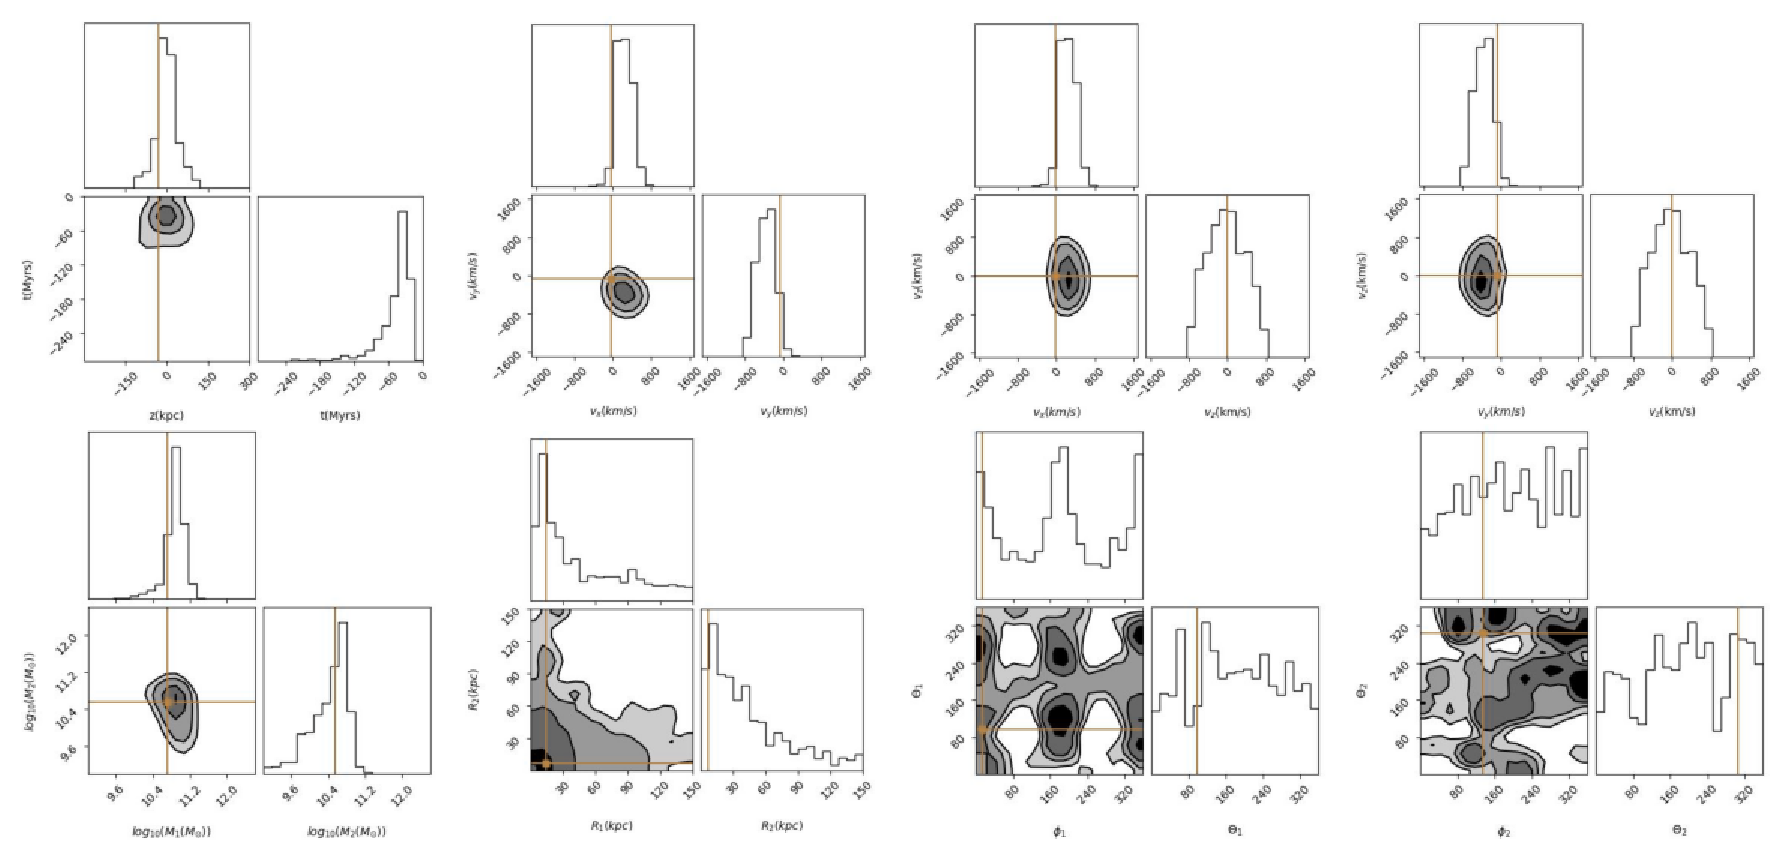
\includegraphics[width=\textwidth]{Chapter1/figures/Arp290-red-corner.pdf}
    \caption[Third example of our best fits from our methodology is representative of the simulated image of Arp 290, a stage 2 system.]{Third example of our best fits from our methodology is representative of the simulated image of Arp 290, a stage 2 system.}
    \label{fig:best-Arp290}
\end{figure*}

\begin{figure*}
    \centering
    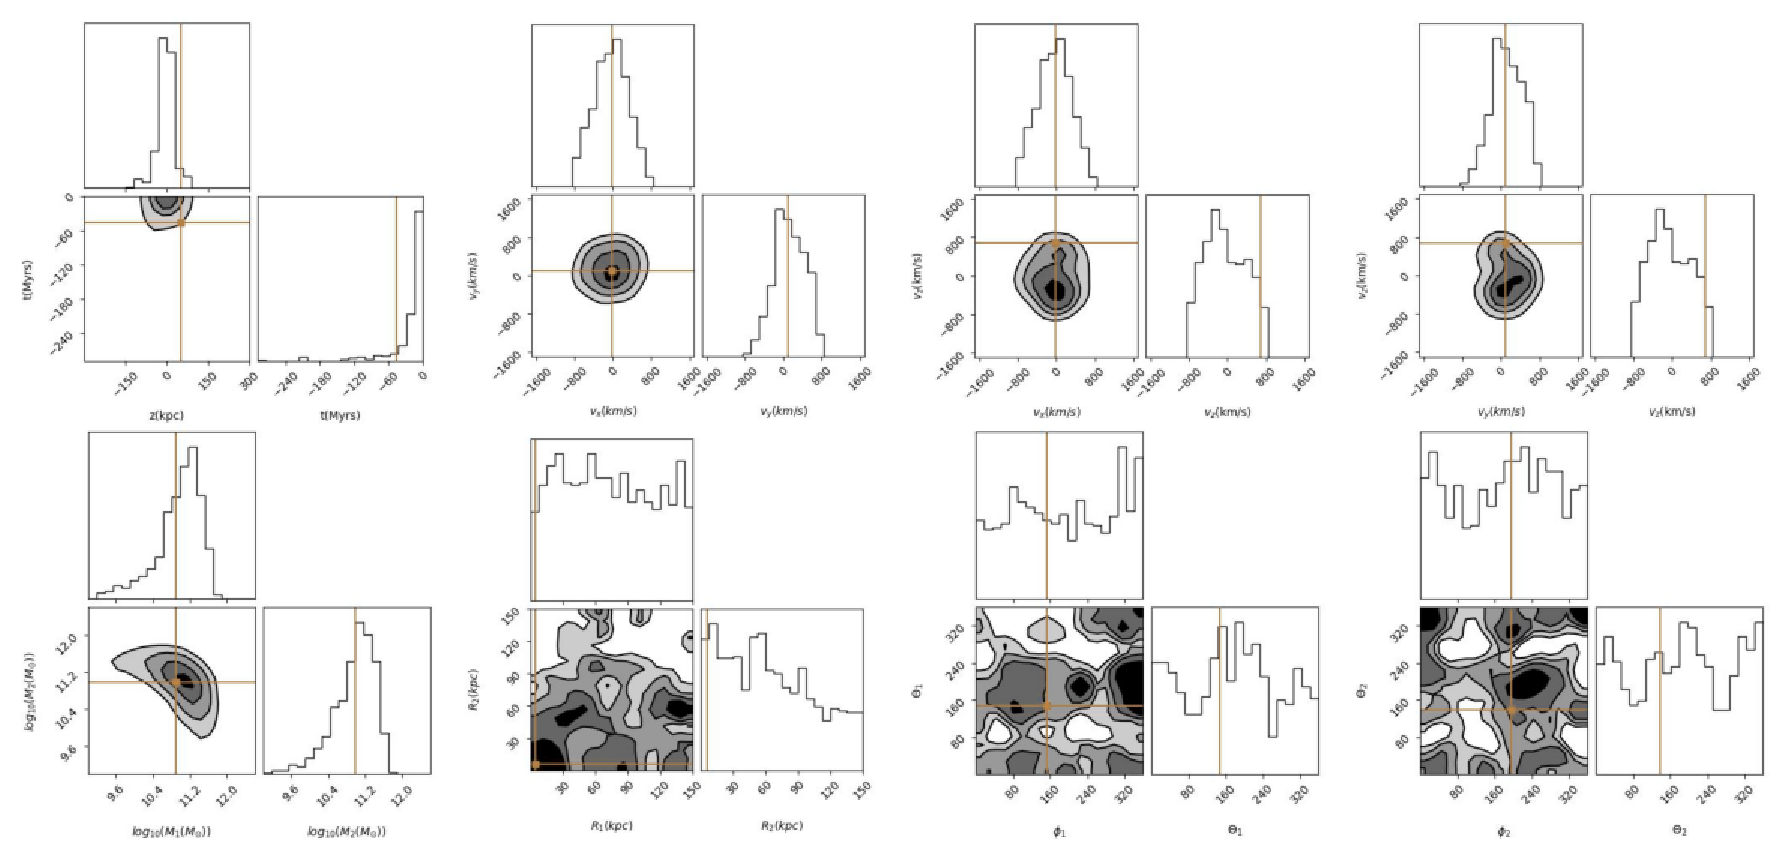
\includegraphics[width=\textwidth]{Chapter1/figures/Heart-red-corner.pdf}
    \caption[First example of our worst fits.]{First example of our worst fits. This shows our constraints of the simulated image of the Heart system, a stage 4 system.}
    \label{fig:worst-Heart}
\end{figure*}

\begin{figure*}
    \centering
    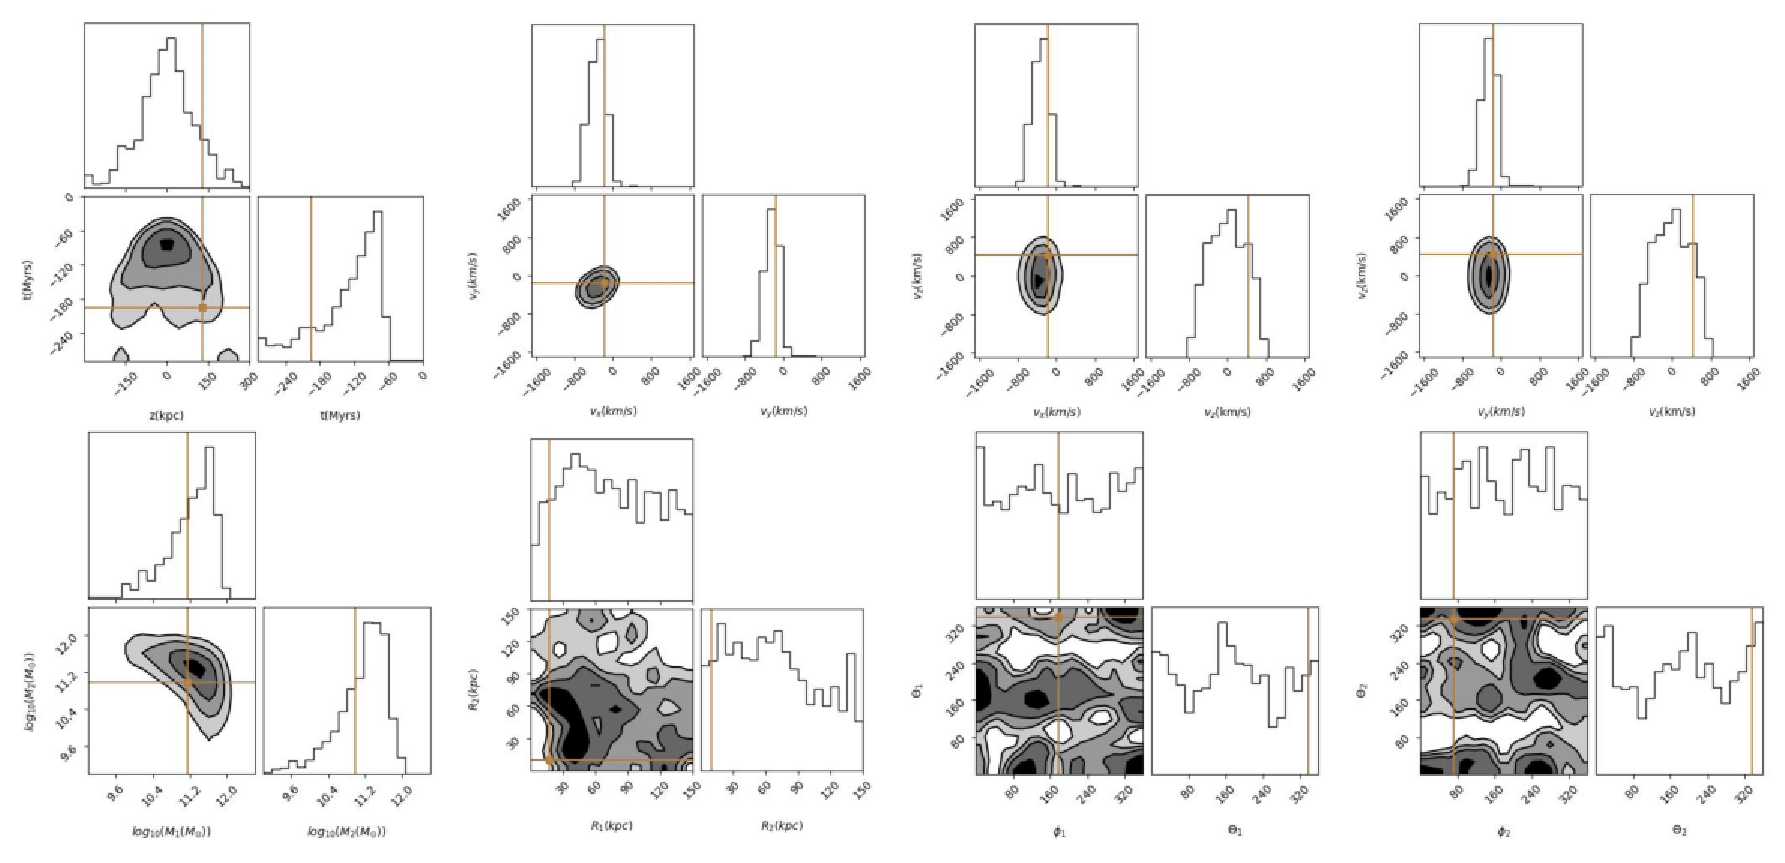
\includegraphics[width=\textwidth]{Chapter1/figures/Arp57-red-corner.pdf}
    \caption[Second example of our worst fits.]{Second example of our worst fits. This shows our constraints on the simulated image of NGC 4320, a stage 4 system.}
    \label{fig:worst-Arp57}
\end{figure*}

\begin{figure*}
    \centering
    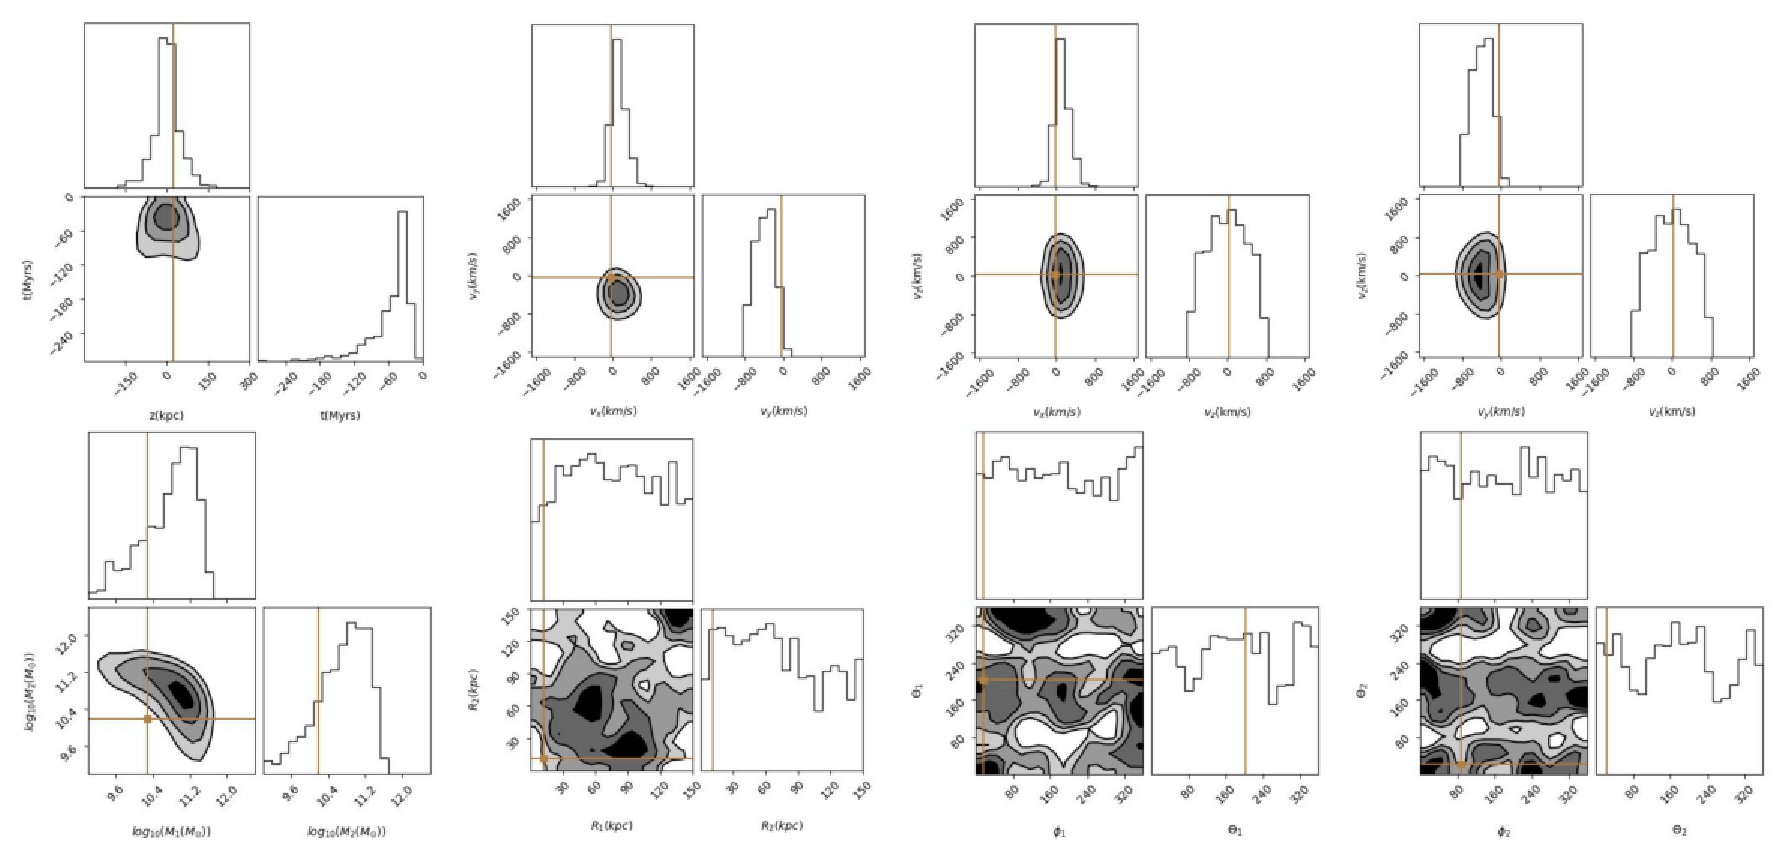
\includegraphics[width=\textwidth]{Chapter1/figures/UGC11751-red-corner.pdf}
    \caption[Third example of our worst fits.]{Third example of our worst fits. This shows our constraints on the simulated image of UGC 11751, a stage 3 system.}
    \label{fig:worst-UGC11751}
\end{figure*}

The worst fits we achieved were of those systems which were close to the merging stage. They were systems where the two cores were close to coalescence, very little tidal features were visible or the position of the secondary galaxy was very unclear. Our worst three fits and examples of this were Heart, NGC4320 and Arp 57. The reduced corner plots are shown in Figures \ref{fig:worst-Heart}, \ref{fig:worst-Arp57} and \ref{fig:worst-UGC11751}. Each of these systems represent the three limitations, respectively. First, is the issue with constraining a stage 4 system. If two cores are close to coalescence, the flux distribution will appear similar to two overlapping disks. Therefore, our $\chi^{2}$ calculation will lead to a maximised likelihood which is equivalent between systems with little to no interaction and a merger with multiple flybys undergoing coalescence. This would be improved by including velocity information, where the velocity distribution will be very different between two overlapping disks and coalescing galaxies. Our process is also not yet designed to account for multiple flybys, which is likely to have occurred in a merging system. To make accurate constraints on many parameters, we require clear and distinct tidal features. UGC 11751 is a system where we have reduced the resolution so much that we lose spatial resolution in the flux distribution of the tidal features. Therefore, we insert a significantly higher uncertainty into our constraints. Finally, our MCMC requires a secondary galaxy to make reasonable constraints on the underlying parameters. The example of NGC 4320 is a final stage merger where a large tidal feature has formed as a result of the coalescence.

% Now, going to break down the generals about each parameter space.
Throughout every system we put constraint on, the parameter we are able to get reliable constraints on are the masses of the systems. This is shown above as even our worst fit systems still hold excellent constraints, with the values confined to small areas of parameter space. However, our worst constraints lie in the orientation and time since the interaction. We show the relation between the true parameter used to create the synthetic image and our recovered best fit parameter with errors included. Figure \ref{fig:true-found-parameters} shows this distribution. We define the best fit value from our MCMC as the 50th percentile of our walker distribution. This is represented by each point in Figure \ref{fig:true-found-parameters}. The upper and lower error bars are calculated from the difference between the 50th percentile value and the 84th and 16th percentile values, respectively. The red lines in each subplot represent a 1-to-1 relation between the true parameter value and the recovered value. 

\begin{figure*}
    \centering
    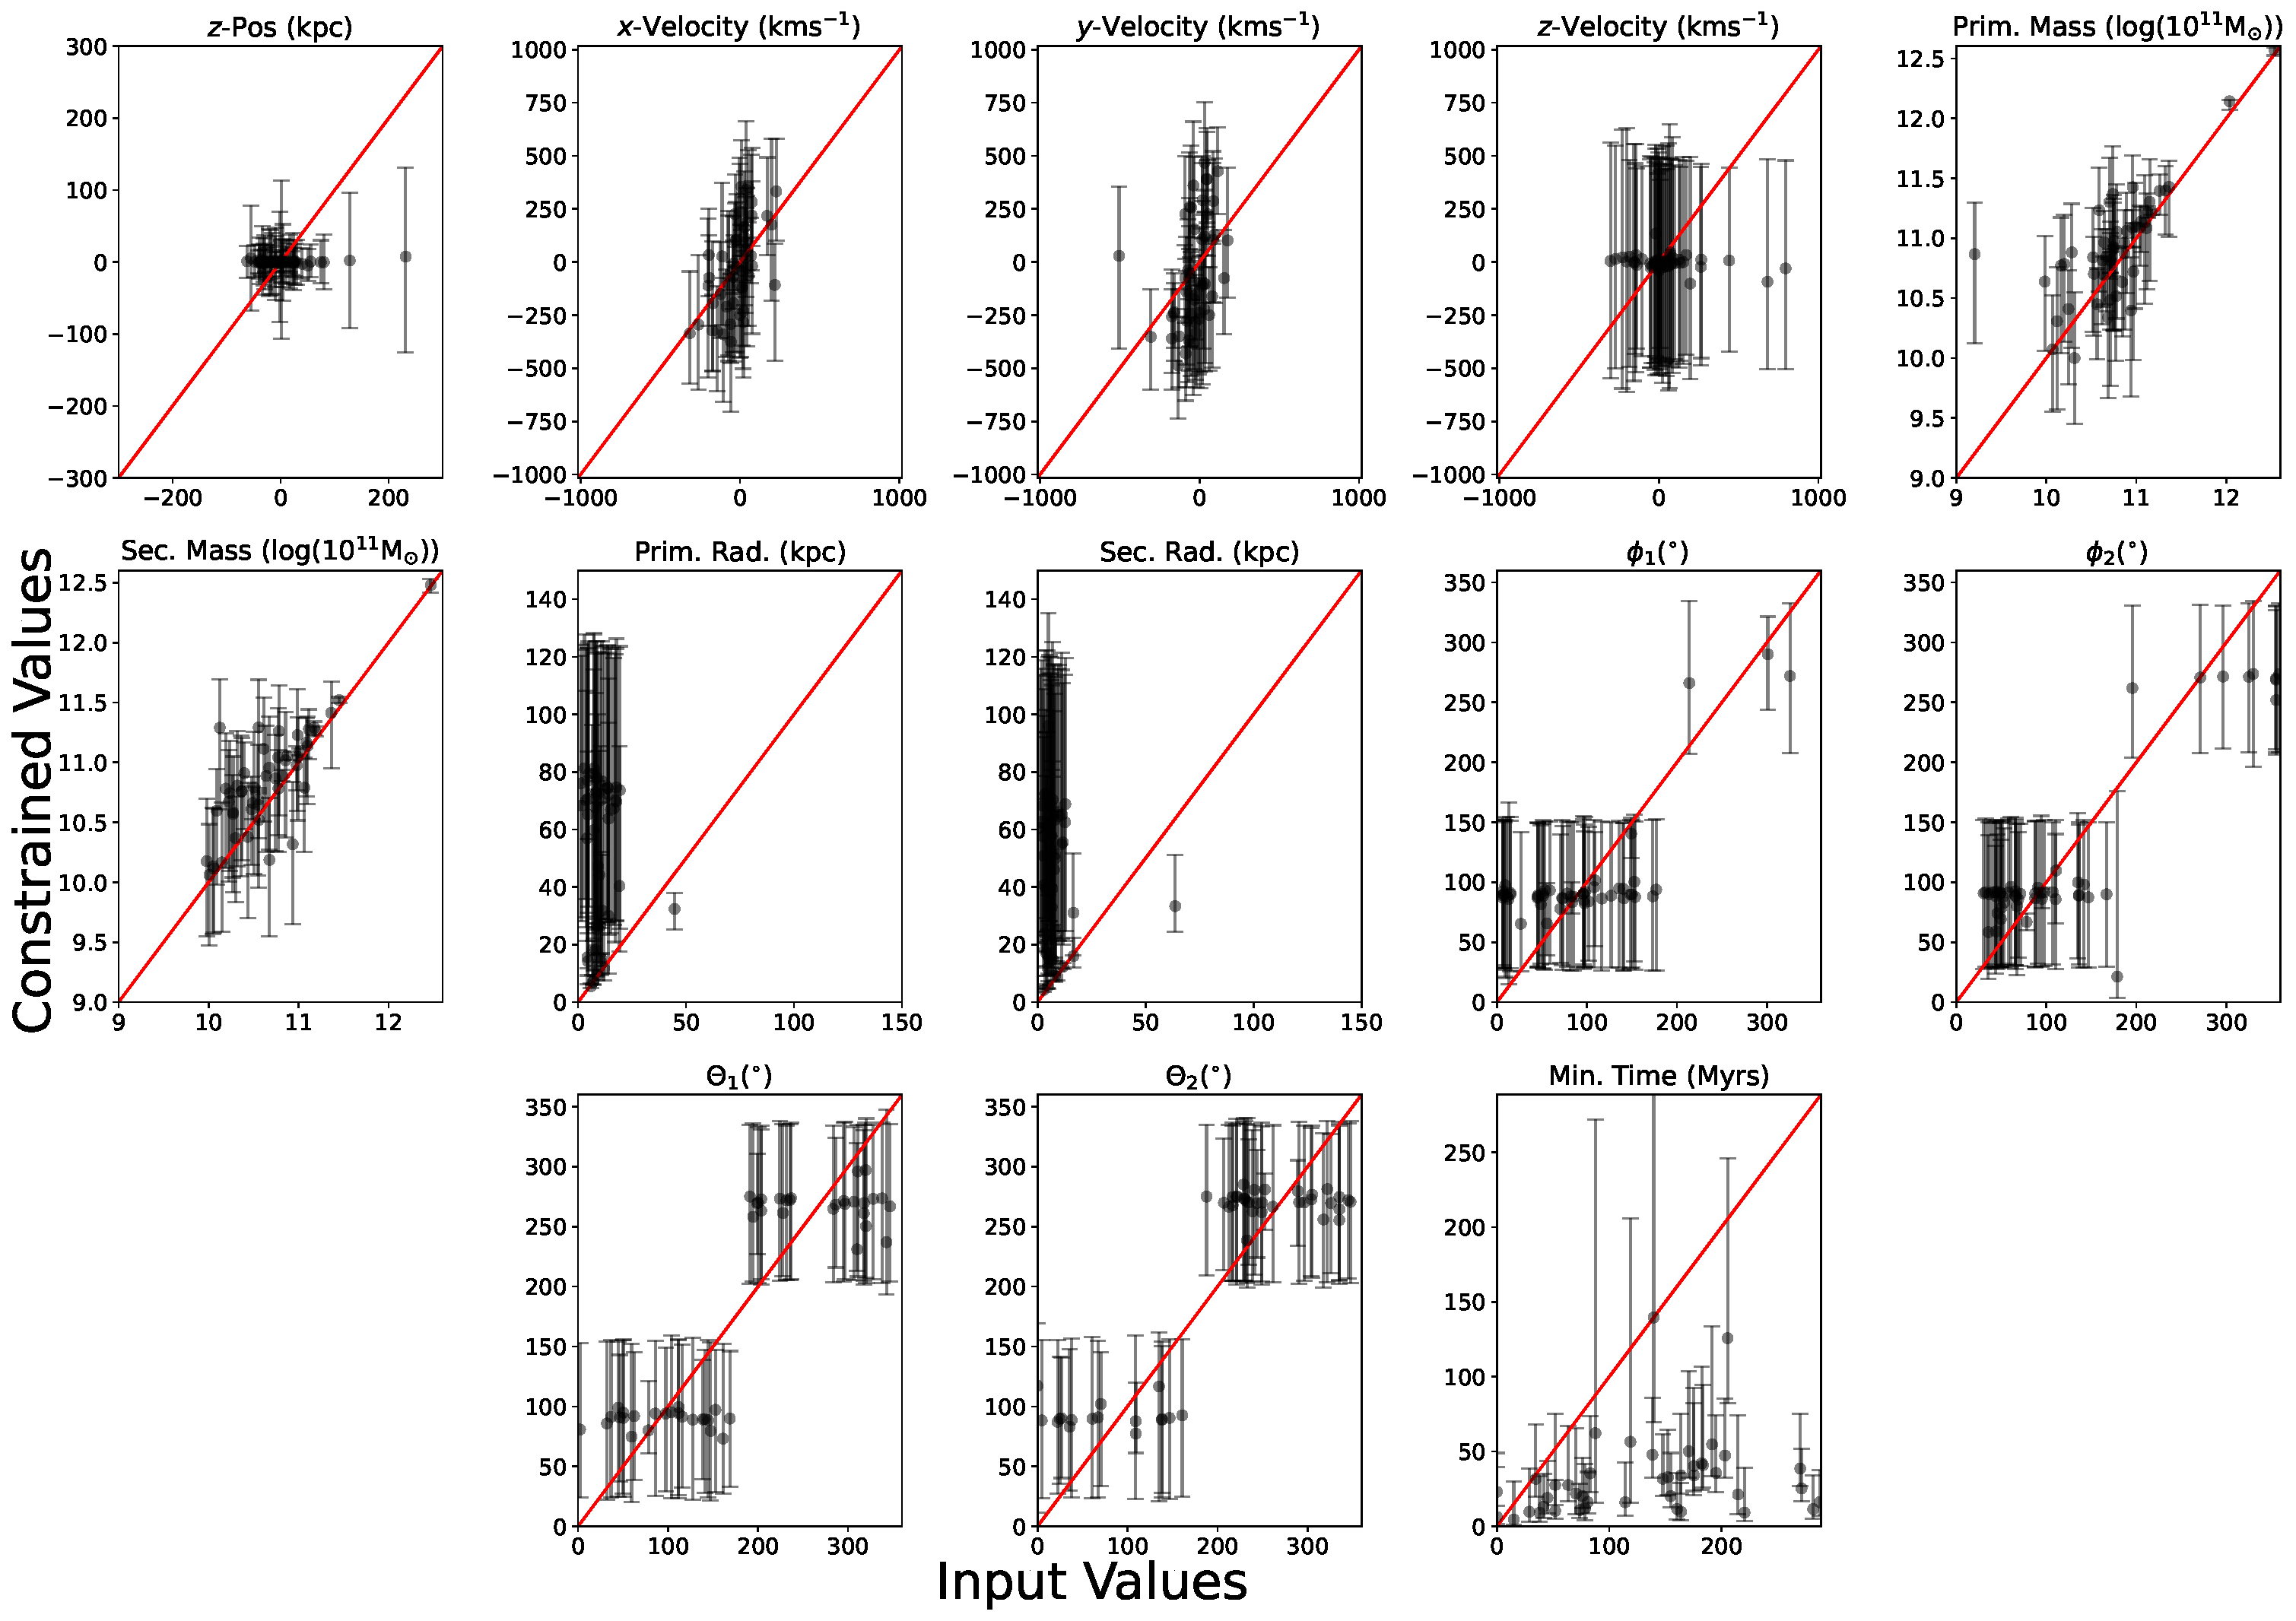
\includegraphics[width=\textwidth]{Chapter1/figures/51_51.pdf}
    \caption[The distribution of parameter values used to create our synthetic interaction images and the best-fit values we recover from our algorithm.]{The distribution of parameter values used to create our synthetic interaction images and the best-fit values we recover from our algorithm. The constrained values are taken as the 50th percentile of our walker distribution. Our lower and upper errors are then calculated as the difference from our best found value and the 16th and 84th percentiles, respectively. This gives an idea of the extent of our walker distribution in 1D. The red lines show a 1-1 relation and where our points would lie if the 50th percentile represented the exact input value found. Parameter names and unts are found in the title of each subplot.}
    \label{fig:true-found-parameters}
\end{figure*}

% Here, discuss Figure 13 in all its glory.
Figure \ref{fig:true-found-parameters} clearly shows where our MCMC has made excellent constraints and where it has not. The best constraints are on the masses of the interacting systems, where each best-fit value approximately follow the 1-to-1 relation. Where there is some discrepancy, the true values are within our errors. There is a trend here, however, that the total mass of the system is over estimated when compared to the true value. We also find excellent constraints on the majority of the positional and velocity vectors of the interaction, where the 50th percentile value approximates the true value. However, in these parameters we have explored a very wide parameter space when the majority of the true values are clustered around the centre of the parameter space. We will require further investigation with interacting systems more representative of the full parameter space we have explored. 

We also have reasonable constraints on our orientation parameters. As we often have two areas of high probability due to degeneracy, we opt to only plot the 50th percentile and errors of the high probability space near the input value. This would not be possible with an observational system with unknown parameters. Therefore, the user will either need to make a choice of what area of parameter space to explore, or input some prior on the orientation / inclination of the system. Once we have accounted for the degeneracy, we find that our 50th percentile value is representative of the true value, with the true value being within error of it. 

There are three parameters remaining where we find poor constraints or struggle to recover the true parameter value in general. The first are the radii of the two galaxies. We find that these are often over-estimated. Upon inspection of many of the output simulations, we find this is likely an effect of the distribution of particles and that we are using idealised synthetic images with no noise in the image. The way in which the particles are distributed is with an exponentially declining disk. This is achieved by creating a disk of particles which are sectioned into rings. Each ring has an exponentially declining probability of particles appearing within it based on the radius from the centre. Therefore, we find the outer rings of the galaxy are diffuse of particles, and do not dominate the likelihood function at high radius. This, in turn, means that galaxies with large angular size can be calculated as likely if the inner parts of the galaxy, with high particle numbers, match the flux of the inner disk. This also explains the over-estimate of the mass of each system. There are likely less particles than expected still within the galactic disk, and therefore more mass (ergo, luminosity) is required to keep the flux matched in the disk.

We also find we often under-estimate the time since the closest point of the encounter - i.e., the time of the passage - by a large margin. While those synthetic images whose underlying parameters had their point of passage very recently we recover very well, those at larger values we fail to. This is due to the likelihood function finding equivalent, high probability values between systems with correct tidal features and simple disks which match the inner disk of the interacting system. The former, tidal feature formation, requires a high $\beta$ parameter with low velocity and low impact distance. However, if the system is fast and does not form tidal features, but ends the simulation in the right place with the correct flux, the calculation will be dominated by the inner disk. Thus, we find a radius that covers the inner parts of the galactic disk successfully, with little disturbance that matches the flux of a large part of the galaxy. Therefore, the $\beta$ parameter is of the utmost importance to filter out these galaxies and give weight to higher t$_{\mathrm{min}}$ values.

Aside from the points that have already been raised regarding our MCMC constraining each parameter, a further problem was that the likelihood calculation is dominated by contributions from the mass and velocity parameters. Therefore, to continue improvements on other parameters further walkers and a longer chain must be run, incurring a cost of far more computation time. For the purposes of this work, we show the full degeneracy, limitations and difficulties of our model and what is to be expected in the most general case. Many of these limitations and problems can be resolved from tighter priors with more information regarding the systems being investigated.

The true power of this approach will be when investigating large populations of interacting galaxies and combining and marginalising over many different posteriors. When combining the parameter spaces of many different systems, it will be possible to identify those areas of parameter space which lead to the formation of certain features across populations of interacting galaxies. Our method will allow more intense simulations to sample smaller parameter spaces and be more efficient when finding systems with specific features. However, how to combine the posteriors is somewhat up for debate. We have ensured that the parameter spaces we are exploring are equivalent in size and that the prior is equal across parameter space. This introduces the question of the $\beta$ parameter in filtering simulations which, indirectly, changes the prior based on the trajectory of the interacting system. To conduct this combination, we would recommend that the $\beta$ parameter was not utilised when building the different posteriors if the increased computational cost is viable.

However, all of our results so far have been in the best-case scenario of a noiseless best fit simulation. The translation from simulation to observation in previous algorithms such as these is never an easy one. We, therefore, use our top three best fit systems here (Arp 172, Arp 240 and Arp 290) and apply our pipeline to their reduced observations.

\subsection{Applying to Observations}
% Brief re-iteration of creating observations.
\noindent We apply our MCMC to the reduced observational data of Arp 172, Arp 240, Arp 256, Arp 290 and Heart. Cutouts were created as described in Section \ref{data:obs-prep}. We reiterate here that the cutout resolution is reduced from its native resolution to cutouts of 100 $\times$ 100 pixels. Before we input the images into the pipeline, we find the central pixel of the secondary galaxy and convert this into a physical $x$- and $y$-position. We also find the total size physical size of the cutout in kpc, convert it to simulation units and provide this to the pipeline. We find that the physical size of the cutouts are significantly different from those of our synthetic dataset. As an example, we create the cutout of Arp 240 at 600 $\times$ 600 pixels at native resolution. With SDSS data, this corresponds to a physical size of 111.50kpc $\times$ 111.50kpc at the redshift of Arp 240. The synthetic image we previously used of Arp 240 is 785.35kpc $\times$ 785.35kpc. Figure \ref{fig:arp240} clearly shows a very different scaling between the observation and simulation, however, it is not enough to be seven times zoomed in on the system. We also find that the secondary positions are very different between the observation image and that used previously. As a result, the parameters we will find for constraining the observation will likely be very different. 

% Why do we take significantly longer on these?
We apply our MCMC to those outputs which had varying constraint. We only investigate these five systems as we find the computational expense is significantly higher when constraining the observations compared to the best fit simulations. We find the reasons for these are two fold. First, we must run each walker for twice the number of steps than when constraining the synthetic images to reach convergence. This is from increased noise contributions in the observation images. Second, due to the smaller scale size of our images, the defined $\gamma$ parameter is much stronger than with the synthetic images. Both of these reasons for higher computational expense are to be expected. The increase in the $\gamma$ parameter leads to us filtering out less candidate systems and running the base simulation code more often. This directly translates into a higher runtime for our MCMC.

% What do we find immediately?
Figure \ref{fig:obs_corner_plot} shows the reduced corner plot for the observed Arp 240 system. The constraints on the velocity parameter have significantly worsened when compared to the constrains on the best fit simulation. They are also in a different area of parameter space when compared. The velocity and spatial parameters are the most likely to be affected by the change in scale between the two input images. As the secondary galaxy position has been completely altered the best fit trajectory of the interaction has also completely changed. The secondary is significantly closer to the primary, therefore meaning the secondary velocity must be significantly slower than previously. Due to the increase in noise in the observational image, and the extent of the tidal features of the primary and secondary galaxies, the constraint has also significantly weakened.

\begin{figure*}
    \centering
    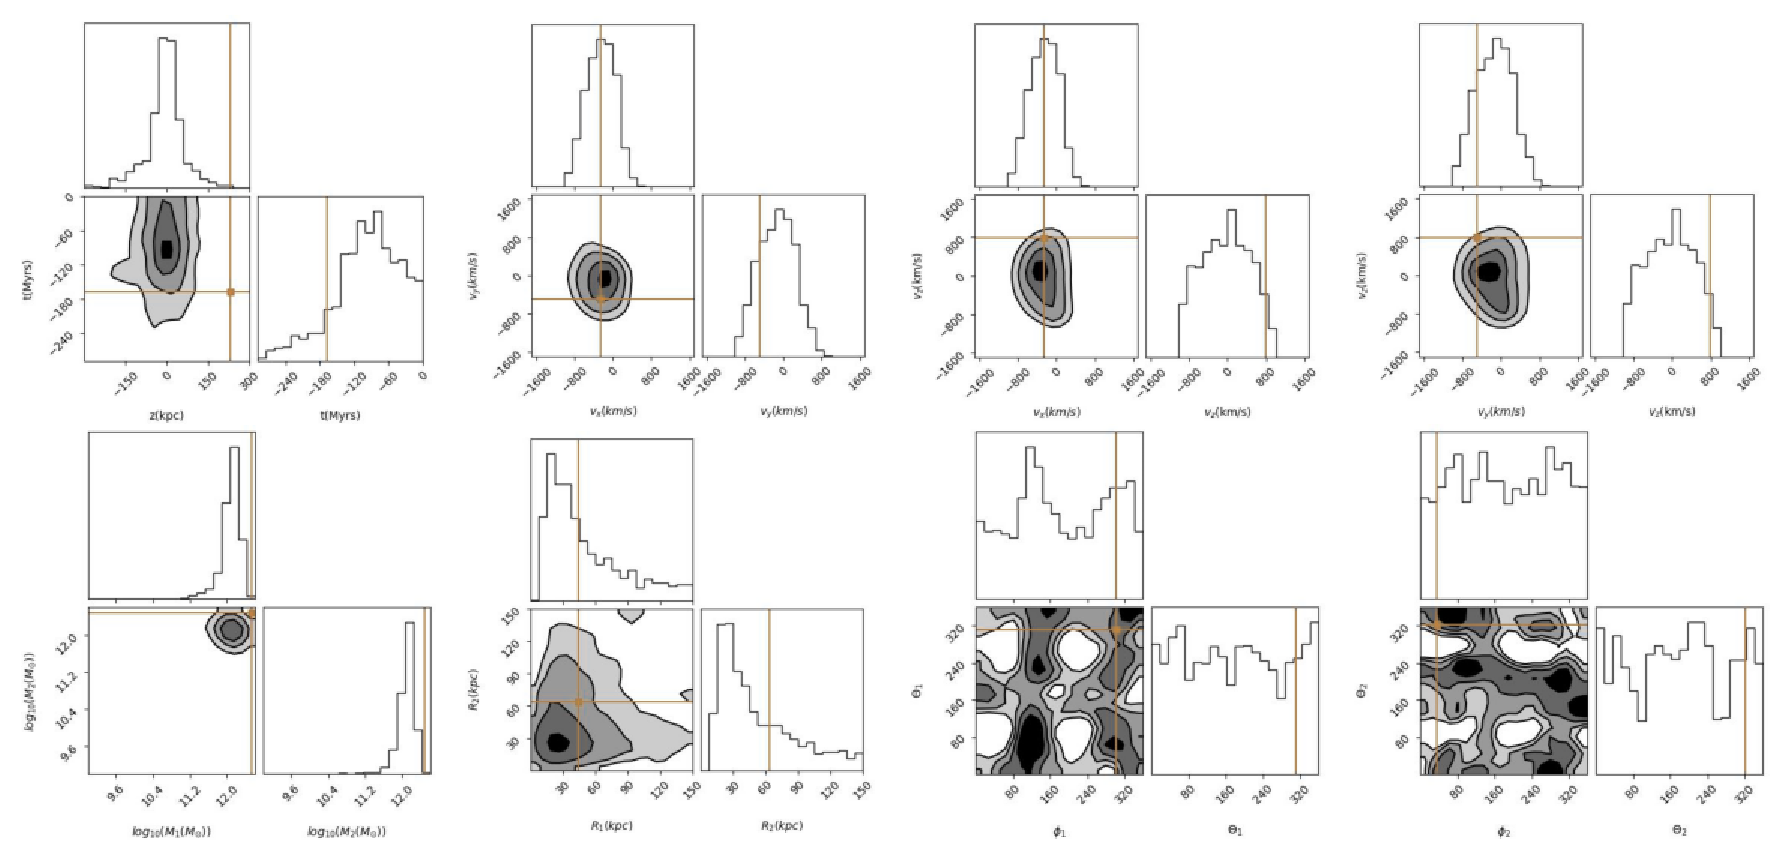
\includegraphics[width=\textwidth]{Chapter1/figures/Arp240_obs-red-corner.pdf}
    \caption[Reduced corner plot of the constraints made on the observational image of Arp 240.]{Reduced corner plot of the constraints made on the observational image of Arp 240. As shown, there is significant additional uncertainty in these measurements than those of the best fit simulation. However, we are able to make constraints on almost all parameters in the sample. The degeneracy in the orientations remains. The gold lines represent the true values we used in to create the synthetic image.}
    \label{fig:obs_corner_plot}
\end{figure*}

However, for the remainder of the parameters the level of constraint remains similar even with the change in the best fit values. We retain the two- and four-fold degeneracy in the orientation parameters. This follows on that the pipeline outright rejects disks which are edge on and loses accuracy when attempting to pin point the precise inclination of each galaxy. We are unable to make any constraint on the $\theta$ parameters, while the degeneracy of the $\phi$ parameters is still visible. The radius parameter is well constrained at 11.8\% CI, although with large tails in the probability space for both the primary and secondary galaxies. These tails are significantly larger here than when using the best fit simulation as the input. This is due to the observation image having no hard cutoff of the edge of the galaxy, and simply moving into more noise. The outer edges of our simulated galaxies also moves to very low signal, and therefore, there is lots of uncertainty surrounding the true radius of the galaxy. 

We, again, make excellent constraints on the mass parameters. The accuracy in the flux distribution of the primary and secondary disk is what dominates here, and therefore, we find this value incredibly quickly. The found value is comparable to the best fit simulation, although slightly lower. We also compare our constrained values to what is found in the literature. Using the criteria described previously, we recover total masses of $\frac{M_{1}}{10^{11}M_{\odot}} = 7.97 - 15.9$ and $\frac{M_{2}}{10^{11}M_{\odot}} = 8.1 - 16.2$ which correspond to stellar masses between $\frac{M_{1,*}}{10^{11}M_{\odot}} =  0.94 - 1.89$ and $\frac{M_{2, *}}{10^{11}M_{\odot}} = 1.0 - 1.9$ in our simulations. These are slightly higher than literature values, with a recent work quoting the stellar mass as $\frac{M_{1, *}}{10^{11}M_{\odot}} = 0.94 $ and $\frac{M_{2, *}}{10^{11}M_{\odot}} = 1.05$ \citep{2020MNRAS.496.5243H}. Thus, while our 50th percentile value is higher than the measured values, we do recover them within error.

This is true in the Arp 172 and Arp 290 observational constraints as well. The synthetic image we have used is at a different scale when compared to the the SDSS observations. We therefore end up with similar constraints to the different parameters, however with significant variation in the spatial parameters. The uncertainties in the radius parameters are significantly increased, while the constraint on the $\theta$ parameters is completely lost. In fact, for the same number of steps compared to constraining the best fit parameters, our MCMC fails the Geweke diagnostic. Therefore, due to the added noise running longer chains is imperative which drives up computational expense.

This leads us onto the limitations of this process to constraining galaxy interaction. While it has been very successful for many of the underlying parameters, there are many different parameters which must be provided to the pipeline so it is able to make those constraints. We discuss the limitations of applying this methodology to large interacting galaxy datasets, and how these can be offset in the short term but a long term solution is still required.

\subsection{Limitations}\label{limitations}
\noindent While this methodology does show a lot of promising in being able to constrain underlying parameters across populations of interacting galaxies, it is important to note that at its base is a restricted numerical interaction code with limited resolution. There may be some interacting systems that simply cannot be modelled realistically using three-body approximations, and may therefore cause a skew in results. However, there are also some more subtle limitations which may affect how a user wishes to use this MCMC approach.

\subsubsection{Resolution \& Depth Effects}\label{resolution_effect}
\noindent One of the fundamental parameters that must be provided for this methodology to work is the redshift of the system. This is used to calculate the distance to the system and then converted to an assumed resolution for the scale of the image. If this is input incorrectly the simulation images will be created at an incorrect resolution, and the MCMC will likely not reach convergence. This is also true of providing and calculating correctly an approximation of the position of the secondary galaxy. Significant computation power can be wasted if these parameters are incorrect, and will give spurious results. The reduction in resolution of the images is also an important limitation. This toy model needs small, thumbnail size images with a reasonable number of degrees of freedom as to reach convergence. Therefore, input images can only be of limited resolution which will affect the quality of the constraints we can actually make on different systems. 

The redshift is also used in scaling the fluxes calculated for each particle in the simulation. The base SED is calculated for a 1 M$_\odot$ system at a distance of 10pc. This is then scaled to the mass assigned to a particle and then put at the distance calculated from the redshift. If the redshift is incorrect (or even slightly off) then this could lead to a bad fit for the mass of the two galaxies in the system. A flag exists in the algorithm to give it the freedom to slightly vary the redshift (and therefore the distance and resolution) by 0.001 with each step. It will then attempt to fit the redshift and resolution of the system. Note, however, this is untested and currently significantly increases computational expense.

Depth effects also play a significant role in the ability of our algorithm to fit a system. For this work, we used primarily synthetic images, meaning we were not at risk of this. However, when using observational imaging this could become a significant problem. Our observational examples were of major interacting systems which resided in the high surface brightness regime, where we retained the full extent of the tidal features and could provide better fitting. However, for systems that lie closer to the low surface brightness regime, our algorithm will become less efficient and require more computational expense to make effective constraints.

This also has the opposite effect in terms of tidal features formed. For example, if a system is being fit but at the true parameters a tidal feature exists which has not been detected due to its low surface brightness then our MCMC pipeline will not be able to converge on the true values. The algorithm would instead converge on those parameters where the disks were at the correct flux rather than getting the tidal features correct. Therefore, when exploring the parameter space of interacting systems with our pipeline, it is imperative that the full structure is within detection of the observing instrument.

There must be a trade off between the resolution of our simulation and the observations. In this work, we used cutouts of 100 $\times$ 100 pixels. This was so that we could still get consistent system outputs from our simulations using only 2500 particles. If lots of pixels are used, then using a low number of particles can lead to many `unphysical' output simulations. I.e. these are simulation systems where the disks will have large holes in them where there haven't been enough particles to fill the disk. To mitigate the effect of potentially using low particle numbers, we distribute the flux as described in Section \ref{flux_dist}, which is an imperfect solution. It is recommended for any user to make a balanced trade off between resolution and computational expense.

\subsubsection{Computational Expense}\label{computational_expense}
\noindent The main drawback of this methodology is that of computational expense required to run such an MCMC over a the full parameter space. In the case of this work, the simulation was set up with 2500 particles on a High End Computer Cluster with 50 CPUS. Each simulation took approximately two seconds, with the full sample run taking approximately 30 days to complete. Each galaxy was given 600 walkers to move through parameter space with each walker moving 7,500 steps. The highest memory requirement of any system was 6GB. Therefore, the runtime is very high but the memory required for it is approximately 122MB per core.

This methodology was successful in constraining 51 different interacting galaxy synthetic images. Achieving the same in prior work projects, such as Galaxy Zoo: Mergers, took months to complete. We have reduced the runtime required of it to 30 days on a powerful High End Computer Cluster. However, this is not the solution to the large scale dataset problems that we will be seeing when LSST comes online. If we are to run this methodology on a much larger galaxy sample - such as thousands of galaxies - then we will need to find ways to significantly improve the runtime of this method.

\section{CONCLUSIONS \& FUTURE WORK}\label{Conclusions}
\noindent In this work, we have introduced a new algorithm based on a MCMC framework to apply constraints on the underlying parameters of interacting galaxies. We have made these constraints, and explored the underlying parameter space, through directly comparing input images to output simulations. Thus, we have mapped the underlying parameters that define interaction to an output morphology that we compare for similarity with a synthetic or observation image of an interaction. We have introduced an updated version of the restricted three body simulation JSPAM and modified it to calculate and match the flux distribution of interacting galaxies based on thirteen underlying parameters. This updated algorithm, APySPAM, calculates the flux distribution by assigning particles with a spectral energy distribution and accounting for star formation throughout the interaction. 

% Look at the tense mash up of the below paragraph.
To test our MCMC, we applied it to a set of synthetic images of interacting systems created from the parameters found in the Galaxy Zoo: Merger project for a set of real interacting systems. We were able to recover the true parameters used to create these images, with associated error measurements on each. We have explored the specific results of a single synthetic image: that of the Arp 240 system, and shown the corner plots and full posteriors of each parameter. We have took the 50th percentile value as the best fit value for our synthetic dataset, and used the 16th and 84th percentile to define the errors on our measurements. We then presented the distribution of our recovered underlying parameters and the true values, describing the general trends in our methodology as well as its limitations. 

Every parameter of our thirteen was recoverable, however there was significant degeneracy in the orientation angles of the two galactic disks. This was expected as works such as \citet{2010ASPC..423..227S} found significant degeneracy between systems, but not a direct cause. In this work we found, without taking account of kinematic information, multiple orientation angles can recreate observed tidal features as well as limitations in the pixel matching method of constraint. When tested on observational data of our best fit synthetic systems, we were able to retain the excellent constraints on nine of the thirteen parameters, but lost any constraint on the orientations. However, we were able to maintain a tight constraint on the masses of the two systems. 

There are limitations to this method that any users must be aware of. First, the core simulation of this process is a restricted three-body code with a highly optimised flux distribution calculation and approximation. It is probable that there are systems that this approach can not constrain, or may give nonphysical results for. The required reduction in the parameter space of the images, such as reducing the degrees of freedom and limiting individual pixel resolution in favour of computation time, also may lead to constraints only on the disks of the galaxies and not the tidal features themselves. There is also limited time and spatial resolution within the simulation itself. When using true observations, they had to be artificially scaled up so our simulation could maintain the resolution to have constraint. In terms of the temporal and spatial parameters, this scale up can be accounted for. However, in terms of the masses of the flux distribution, this can be significantly hindered. Therefore, a user must be careful when choosing the image scales to use when attempting to constrain individual systems. 

We have demonstrated the power of this methodology, and that it is capable of recovering the underlying parameters of interaction in idealised examples. The next, serious test of this MCMC approach will be to use it on a set of observed interacting systems, where the underlying parameters are known to properly diagnose the results. However, completely constrained interacting galaxy samples are only of a small scale and few exist. We will apply our MCMC to the observed dataset of our 51 interacting systems in SDSS.

This is an initial step towards developing the methodology to serve the field as large scale surveys - such as LSST - come online. Large scale automation where we can constrain interaction, make diagnostics and estimates about parameter space are not only important for inferences about individual datasets but for the interacting galaxy population as a whole. The main limitation of this method is the computational expense associated with it. To run this on 51 systems, the total run time was thirty days; an unusable timescale when being applied to interacting galaxy samples in the thousands. Therefore, future works with this algorithm and methodology will also be focused on increased computational efficiency and working on larger interacting galaxy datasets. 

The bottleneck for computational efficiency lies in the time spent running the APySPAM simulation. While incredibly cheap individually, this is exceptionally expensive when having to be run in an MCMC chain. With the growing power of GPUs, and their ability to run numerical simulations significantly more efficiently than CPUs, a pathway to solve this limitation may already exist. This, combined with further developments in methodologies such as simulation based inference, machine learning and gaussian processes could begin to reduce computation time.
\chapter{Advanced PySPAM: An Infrastructure to Constrain Underlying Interacting Galaxy Parameters}\label{chapter4}
\section{Introduction}\label{Introduction}
% Introduce interaction, and why it's important.
\noindent The precise interplay between the observed processes we have discussed in this thesis and the underlying physical parameters of the involved galaxies is difficult to quantify. Using large scale observational datasets allows us to probe this relation, but without the ability to constrain the dynamical timescale the precision of our constraints on it remains limited. Algorithms have been developed to match the underlying parameters of an interaction and its dynamical timescale by directly modelling the expected final morphology. If a simulation of an interaction can reproduce the final morphology, then it has likely correctly inferred the interaction over the dynamical time.

Examples of algorithms designed to make this matching include Identikit by \citet{2009AJ....137.3071B} or the Stellar Particle Animation Module (SPAM) by \citet{1990AJ....100.1477W}. However, finding the best fit underlying parameters for more than a handful of systems is often seen as unfeasible. There are often greater than 10 different parameters which contribute to different observed morphologies. This leads the underlying parameter space to be greater than 10-dimensional and complex. Exploring even a sub-space of this parameter space fully requires tens of thousands of models to be run. This is also hindered by its degeneracy. For example, \citet{2010ASPC..423..227S} found that four of their best-fit models were able to accurately match morphology of the Arp 284 system. Therefore, it is often preferable to use large cosmological simulations \citep[e.g.][]{2015MNRAS.446..521S, 2018MNRAS.480..800H, 2020MNRAS.493.3716H} to create large samples of synthetic interacting galaxies where analogues to the observed system can be found. This, however, limits our capability to explore observational parameter space beyond the limitations of such cosmological simulations. By their nature, cosmological box simulations have finite scope and size; meaning the rarest (and likely most fundamental) interacting systems will remain unexplored without significant further computational expense.

This limitation of directly comparing numerical simulations to observations was solved in a novel way by \citet{2016MNRAS.459..720H} in the Galaxy Zoo: Mergers (GZM) project (for details on Galaxy Zoo, see \citet{2008MNRAS.389.1179L}). GZM worked with citizen scientists to run simulations of interaction and visually compare the simulated morphology to observations. GZM studied a sample of 62 interacting galaxies from the Arp catalogue of interacting galaxies \citep{1966ApJS...14....1A}. Citizen scientists' were given a selection of simulation outputs around an observation and would select the one which appeared most alike. The simulations would then be run again with tweaked underlying parameters with the citizen scientist selecting the new the best fit output. With enough citizen scientists on the project, enough new simulations run and enough time GZM were able to find the best fit parameters for their interacting galaxy sample across a 14-dimension parameter space. This created the largest fully constrained interacting galaxy samples to date. In the era of the Vera C. Rubin Observatory such an approach will not be practical, with statistically significant samples of thousands of interacting galaxies potentially being produced every week, a new approach is required.

In this Chapter, we present an automated methodology to constrain the underlying parameters of interaction. We combine a fast restricted numerical simulation code with a Markov-Chain Monte Carlo (MCMC) framework. We apply this over a 13D parameter space and constrain the probability distribution and find the likely parameter values describing an interacting galaxy system. This approach allows us to marginalise over each parameter, provide the best fit value as well as the error on each measurement. First, we apply this to a set of synthetic interacting galaxy observations created from a restricted N-body simulation where we have input the 13 underlying parameters. This provides us with diagnostics of our methodology. We then apply our process to five real observations of interacting galaxies and discuss how our methodology could be applied to real data, and the limitations therein. We also discuss the more general limitations of this approach, with a particular emphasis on the computational expense required, and the potential future solutions.

% Layout of document/
The layout of this Chapter is as follows. In Section \ref{Data}, we describe the sample of 51 galaxies we will study and our approach to observation preparation. Section \ref{Methods: sims} will summarise our simulation code and how it has been updated from previous iterations. We also describe how we build our sample of synthetic interacting galaxies and the parameter space we will explore with this simulation. A full discussion of our results will be given in Section \ref{Results} followed by our conclusions and future work in Section \ref{Conclusions}.

\vspace{-5mm}
\section{Data}\label{Data}
% What is the data?
\subsection{Sample of Major Interacting Galaxies}
\noindent In this work, we test our Markov-Chain Monte Carlo (MCMC) process on idealised, mock observations of 51 major interacting systems. These mock observations are created using our numerical simulation where we have input the underlying parameter values directly. As we know what the true underlying parameters of each interaction are, we can test the accuracy of our MCMC. To create these mock observations, we use the underlying parameters found in the GZM project for 62 interacting galaxies.

Of the 62 systems, we create synthetic images of 51 of them to act as our idealised observational sample. As we are including the flux distribution of each system, we require an accurate redshift of each system. 3 of the 62 systems do not have a redshift measurement in the NASA Extragalactic Database (NED), the Sloan Digital Sky Survey (SDSS) or Simbad databases. Therefore, we discard these. We create each mock observation as though it was observed using SDSS. Of which, a further eight systems are not present. Therefore, we also discard these systems. This leaves us with the GZM best-fit parameters of 51 systems with which to create our synthetic observations. The details of the real systems are displayed in Table \ref{tab:Objects}, including the target coordinates, the SDSS ID and the redshift measurements we use. How we create our synthetic images is described in Section \ref{sec:syn_sample} after we have described our simulation.

\begin{table*}
    \centering
    \resizebox{0.79\textwidth}{!}{\begin{tabular}{|c|c|c|c|c|c|c|}
    \hline
         Name & SDSS ID & RA & Dec & Redshift \\
         \hline
         Arp 240 & 587722984435351614 & 204.980417 & 0.835278 & 0.02250 \\
         Arp 290 & 587724234257137777 & 30.946317 & 14.72365 & 0.01171 \\
         Arp 142 & 587726033843585146 & 144.429583 & 2.763056 & 0.02329 \\
         Arp 318 & 587727177926508595 & 32.380516 & -10.158508 & 0.0132 \\
         Arp 256 & 587727178988388373 & 4.710417 & -10.369167 & 0.02730 \\
         UGC 11751 & 587727222471131318 & 322.247796 & 11.382539 & 0.02909 \\
         Arp 104 & 587728676861051075 & 203.037083 & 62.733889 & 0.01082 \\
         Double Ring, Heart & 587729227151704160 & 238.287292 & 54.147861 & 0.040 \\
         Arp 285 & 587731913110650988 & 141.040000 & 49.226111 & 0.00967 \\
         Arp 214 & 587732136993882121 & 173.145221 & 53.067922 & 0.00331 \\
         NGC 4320 & 587732772130652231 & 185.740516 & 10.548328 & 0.02668 \\
         UGC 7905 & 587733080814583863 & 190.952917 & 54.900278 & 0.01648 \\
         Arp 255 & 587734862680752822 & 148.290000 & 7.870000 & 0.04106 \\
         Arp 82 & 587735043609329845 & 122.811250 & 25.193056 & 0.01368 \\
         Arp 239 & 587735665840881790 & 205.423852 & 55.672324 & 0.02489 \\
         Arp 199 & 587736941981466667 & 214.265833 & 36.573333 & 0.01024 \\
         Arp 57 & 587738569246376675 & 199.198750 & 14.424444 & 0.048 \\
         (HWB2016)Pair 18 & 587738569249390718 & 206.209583 & 13.921361 & 0.089 \\
         Arp 247 & 587739153356095531 & 125.889478 & 21.342976 & 0.01108 \\
         Arp 241 & 587739407868690486 & 219.461958 & 30.481222 & 0.03472 \\
         Arp 313 & 587739505541578866 & 179.418333 & 32.285556 & 0.01045 \\
         Arp 107 & 587739646743412797 & 163.069583 & 30.065278 & 0.03318 \\
         Arp 294 & 587739647284805725 & 174.931624 & 31.920108 & 0.00892 \\
         Arp 172 & 587739707420967061 & 241.389583 & 17.597222 & 0.029 \\
         Arp 302 & 587739721376202860 & 224.251667 & 24.612222 & 0.03286 \\
         Arp 242 & 587739721900163101 & 191.544583 & 30.727222 & 0.02205 \\
         Arp 72 & 587739810496708646 & 236.733750 & 17.878333 & 0.01100 \\
         Arp 101 & 587739845393580192 & 241.124946 & 14.800192 & 0.026 \\
         Arp 58 & 587741391565422775 & 127.990209 & 19.211523 & 0.03722 \\
         Arp 105 & 587741532784361481 & 167.804167 & 28.724722 & 0.021 \\
         Arp 97 & 587741534400217110 & 181.439583 & 31.068889 & 0.02305 \\
         Arp 305 & 587741602030026825 & 179.655833 & 27.490833 & 0.004 \\
         Arp 106 & 587741722819493915 & 183.902522 & 28.173576 & 0.02199 \\
         NGC 2802/3 & 587741817851674654 & 139.172619 & 18.963463 & 0.02914 \\
         Arp 301 & 587741829658181698 & 167.470000 & 24.259722 & 0.02059 \\
         Arp 89 & 587742010583941189 & 130.665852 & 14.285624 & 0.00687 \\
         Arp 87 & 587742014353702970 & 175.185000 & 22.437778 & 0.02373 \\
         Arp 191 & 587742571610243080 & 166.834167 & 18.431111 & 0.02739 \\
         Arp 237 & 587745402001817662 & 141.933458 & 12.286750 & 0.02899 \\
         Arp 238 & 588011124116422756 & 198.886667 & 62.126944 & 0.03106 \\
         MCG +09-20-082 & 588013383816904792 & 181.161667 & 52.956111 & 0.078 \\
         Arp 297 & 588017604696408086 & 221.330417 & 38.761389 & 0.0298 \\
         NGC 5753/5 & 588017604696408195 & 221.328663 & 38.805889 & 0.01374 \\
         Arp 173 & 588017702948962343 & 222.869434 & 9.328297 & 0.028 \\
         Arp 84 & 588017978901528612 & 209.649167 & 37.438889 & 0.01158 \\
         UGC 10650 & 588018055130710322 & 255.060770 & 23.106346 & 0.00986 \\
         Arp 112 & 758874299603222717 & 0.368333 & 31.437778 & 0.024 \\
         Arp 274 & 587736523764334706 & 218.786250 & 5.356389 & 0.02890 \\
         Arp 146 & 587747120521216156 & 1.685000 & -6.635833 & 0.07544 \\
         Arp 143 & 588007005230530750 & 116.72333 & 39.019444 & 0.01374 \\
         Arp 70 & 758877153600208945 & 20.864583 & 30.778333 & 0.03500 \\
         Arp 218 & 587739720308818095 & 238.397500 & 18.607222 & 0.075 \\
         \hline
    \end{tabular}}
    \caption[The names, SDSS ID, right ascension, declination (in degrees) and redshift for the 51 interacting systems we will examine.]{The names, SDSS ID, right ascension, declination (in degrees) and redshift for the 51 interacting systems we will examine. All redshifts are as found on the NASA Extragalactic Database.}
    \label{tab:Objects}
\end{table*}

\subsection{Observation Preparation}\label{data:obs-prep}
\noindent To robustly test our MCMC algorithm, we will constrain the underlying parameters of observations of a subset of the systems described in Table \ref{tab:Objects}. Therefore, we describe how we build such observational images here. We downloaded the FITS files from SDSS Data Release 16 which contained the full system of interacting galaxies. These were then used to create smaller cutouts of the systems. The coordinates of the primary galaxy are used as the center of the image. We judged the size of the cutout by the size of the full interacting system, most often between 600 - 1000 pixels. We created cutouts in each SDSS filter ($ugriz$).

We convert each observational image into counts from the native unit of nanomaggies using the conversion value in each FITS header. Each filter image was then stacked into white image by simply summing them together. This gave us a higher signal-to-noise in the tidal features of the interacting systems. Then, we took these native resolution white images and block reduced them to a 100 $\times$ 100 thumbnail. Each cutout was visually inspected to ensure that, even with the reduced resolution, the tidal features were still clear and prominent in the image.

We take the 0.396" pixel scale of SDSS on the sky with the measured redshift to calculate its physical size. From the pixel-to-distance conversion for each image, the position of each secondary galaxy was calculated from the central pixel. No attempt was made to approximate the $z$-position of the secondary galaxy, as this is a parameter to constrain. In total, there are 13 parameters that we must constrain over our synthetic and observation images. These parameters are detailed in the following section. The observation image preparations were made using the Astropy Python package \citep{astropy_2013, astropy_2018}.

% Describe what GZ: Mergers found and what we're going to do that is different.
% This should perhaps be in the Introduction if it isn't already.
\section{Simulating Galaxy Interaction}\label{Methods: sims}
\noindent We require a method of mapping underlying parameters to our observed systems morphology and calculating how likely it is they are representative. We input our set of underlying interaction parameters into a restricted three-body simulation which predicts the morphology and flux distribution of the interacting system. In this section, we describe our simulation code, its previous iterations and how we add in additional flux information.

\subsection{APySPAM}\label{sec:simulations}
% What is it?
\subsubsection{Restricted Three-Body Simulation}\label{sec:apyspam}
The simulation code we use is the Java Stellar Particle Animation Module (JSPAM) \citep{2016A&C....16...26W}. For an in-depth description of the underling code, we direct the reader to \citet{1990AJ....100.1477W,2016A&C....16...26W} but provide a summary here. JSPAM is a restricted three-body code focused on recreating the morphology of interacting systems. It approximates the interaction as two massive bodies each being orbited by a set of massless test particles. The gravitational potential of the two massive bodies and the resultant forces upon the massless test particles is calculated and used to predict the particles position and velocity at different timesteps. The size and number of time steps can be input by the user. JSPAM is computationally efficient, approximating the morphology of an interacting system using thousands of particles in seconds on a regular work PC at a reasonable time resolution. The primary particle integrator is a fourth-order Runge-Kutta which applies backwards integration to calculate the position and velocity of the massive bodies from t=0 to the time set by the user. The test particles are then added to the simulation, and forward integration is conducted to find their position and velocity in each timestep through the trajectory of the massive bodies. In this way, a flyby of the two galaxies is simulated with the test particles representing the extended morphology of the two galaxies. 

The user has the option to choose a N-body approximation or a softened point mass approximation. Each of these slightly changes the way that the integrator calculates the forces on each particle. Therefore, there will be slight discrepancies between the final morphology of systems interacting with the same underlying parameters but different force approximations. We elect to utilise the softened point mass approximation, as this has improved computational efficiency over the higher accuracy of N-body approximation \citep[for more on this see][]{2016A&C....16...26W}. 

The base code of JSPAM was purely a morphology matching code. Attempting to extract underlying parameters of interaction from morphology matching alone has been shown in prior works to be difficult \citep[e.g.][]{2009AJ....137.3071B}. JSPAM itself has been used in genetic algorithms to find the best fit parameters of different systems \citep[e.g][]{2023A&C....4200691W}. However, this lacks the exploration of parameter space and the quantification of uncertainties we aim to achieve in our approach. Using both morphology and flux matching between simulations and observations improves accuracy of recovered parameters \citep{2021ApJ...923..124M} and we have therefore enhanced the original JSPAM algorithm with the ability to model population evolution with star formation/star bursts to approximate the flux distribution of the interacting system. We have created this enhanced version in Python 3.7.4 (hence, we shall refer to this algorithm as Advanced Python Stellar Particle Animation Module, APySPAM).

To approximate the flux distribution of the galaxies in the simulation we calculate luminosity of each particle while minimising the computational cost. We incorporate the evolution of the underlying stellar populations of each galaxy over the time taken in the interaction. We also incorporate the formation of new stellar populations in potential starbursts, and approximate the impact this will have on the galaxy flux distribution. To preserve the computational efficiency, we build a semi-analytic model and define a global stellar population to assign a luminosity to each particle based on its assigned, hypothetical mass. In this way, we `paint on the stars' of each galaxy without having to directly model stellar evolution and star formation. This process is detailed in the following two subsections. 

% Why is it different from the original JSPAM?
% Overview of APySPAM:
\subsubsection{Stellar Population Evolution}\label{Stellar_Pop_Evol}
To model the underlying stellar populations, we utilise a \citet{2003MNRAS.344.1000B} (BC03) simple stellar population. These contain SEDs generated from flux libraries from a \citet{2003PASP..115..763C} initial mass function. We set this stellar population model to have a delayed exponentially declining star formation rate \citep{2009ApJ...690..802J, 2013ApJ...762L..15P,2014arXiv1404.0402S, 2019A&A...622A.103B}. However, to capture any star formation due star formation enhancement in the interaction, we increase the star formation based on the conditions in the interaction. We assume an e-folding time for star formation of $\tau = 1.7\text{Gyrs}$. This value is chosen as it matches field, massive galaxies found in the literature \citep[e.g][]{2010ApJ...721..193P} and used in hydrodynamical simulations \citep[e.g.][]{2022ApJ...941....5J}. Our simulation outputs a spectrum normalised to 1M$_{\odot}$ with each particle initially assumed to be the same age as the galaxy.

This spectrum must then be scaled to the stellar mass present at each particle. We follow the prescription as stated in \citet{2016A&C....16...26W} to distribute the mass between the three components of the galaxy, and then to each test particle. The galaxy in the JSPAM simulation has its mass distribution as $M_{\text{bulge}} = 0.05M_{\text{galaxy}}$, $M_{\text{disk}} = 0.14M_{\text{galaxy}}$ and $M_{\text{halo}} = 0.81M_{\text{galaxy}}$. We take the total mass assigned to the galaxy (input by the user) and divide it into these three components. We then assume that the bulge and disk masses are fully baryonic, with the remaining mass being non-baryonic dark matter. We further divide the calculated baryonic mass into two components: stellar and gas. The total stellar mass of each particle is used to scale our final output SEDs from our model while total gas mass of each particle is used to calculate the star formation rate. The gas and stellar mass to be distributed to the particles is then defined by a gas fraction parameter that the user can alter. By default, this value is 0.15 for both the primary and secondary galaxies.

We assume the initial ages of the galaxies (both 10Gyrs by default) at initialisation and calculate the final age of the SEDs based on the number of time units the user wishes to run the simulation. This age is then used to extract the normalised spectra from the BC03 templates. These output SEDs are then convolved with given telescope filters of the users choice and integrated, giving a colour flux value to each particle. However, this process only outputs the final flux values at each particle of the initial stellar population. During the interaction, we assume that the galaxy begins to form new stars at a rate significantly higher than is modelled in the BC03 templates. Therefore, we account for this by modelling newly created stellar populations as the interaction progresses.

To incorporate the increase in star formation in our simulations, we manually enhance the expected star formation rate through the simulated interaction. In high-resolution simulations which also model the evolution of gas, starbursts occur naturally \citep{2009PASJ...61..481S}. However, in our simulations we must approximate this behaviour in a semi-analytic fashion. The change in star formation is heavily dependent on the mass ratio and the kinematics of the interaction and, therefore, we implement an enhancement parameter based on these parameters. We calculate the excess star formation due to the interaction compared to what is already expected in the SED, and distribute this to each particle based on the initial gas mass. Approaching the problem in this semi-analytic way is similar to what is done in the CIGALE \citep{2019A&A...622A.103B} algorithm. Here, we detail this enhancement parameter.

At any given timestep the total stellar mass is given by
\begin{equation}\label{Total_SFR}
    SFR_{\text{enhancement}} = \beta (\frac{t}{\tau^{2}}) \exp(-\frac{t}{\tau}) M_{\text{baryonic}} M_{\odot} \text{yr}^{-1}.
\end{equation}
Here, $\tau$ is the e-folding time of star formation, $M_{\text{baryonic}}$ is the baryonic mass of the galaxy and t is the age of the galaxy at the given timestep. This is the star formation at any time given by the BC03 template. However, we include the $\beta$ parameter: our enhancement value. This is a dimensionless value given by
\begin{equation}\label{enhancement_param}
    \beta = M_{\text{ratio}} D_{\text{ratio}}^{2}.
\end{equation}
$M_{\text{ratio}}$ is the mass ratio between the galaxy being enhanced and the galaxy causing the interaction. D$_{\text{ratio}}$ is the ratio of each galactic radius to the distance between the galactic cores. In a system with a high mass galaxy interacting with a low mass galaxy, the high mass galaxy will have relatively little star formation enhancement while the less massive galaxy will have significant enhancement. This is similarly true for the ratio of the radius and separation. If the galaxies are interacting in such a way that the distance of closest approach is less than each galactic radius, then this ratio will rapidly increase above one; enhancing star formation further. This represents a significantly more violent interaction. It is important to note, however, that this has significantly less impact on strengthening star formation than that of the mass ratios. 

These parameters successfully reflect the findings of the current astrophysical literature, where mass ratio has a significantly higher role on star formation enhancement than impact parameter \citep{2003ApJ...582..668B, 2008MNRAS.391.1137L, 2008MNRAS.385.1903L}. We base our semi-analytic approach on the star formation histories found in a range of high resolution N-body simulations \citep{1996ApJ...464..641M, 2000MNRAS.312..859S, 2019MNRAS.490.2139R} which measure the change in star formation directly from the Kennicutt-Schmidt \citep{1998ApJ...498..541K} relation. These simulations directly model the star forming gas through the interaction, measuring the change its evolution which we are able to approximate. Thus, we achieve an accuracy comparable to directly-modelled simulations at a fraction of the computational cost.

The output of Equation \ref{Total_SFR} is global star formation of each interacting galaxies at any given timestep. However, the aim of our model is to be able to match the flux distribution across the entire galaxy (particularily the tidal features) to any observation that the code is given. Therefore, we must distribute the star formation throughout the particles. To keep computational efficiency, we utilise weights which have been assigned to each particle. These weights are based on the ratio of the gas mass of the particle which has been assigned at initialisation to the total gas mass of the galaxy. So, to find the star formation rate of a single particle at any given timestep, the following equation is applied,
\begin{equation}
    SFR_{\text{Particle}} = \frac{M_{\text{gas,Particle}}}{M_{\text{gas,Galaxy}}}SFR_{\text{Galaxy}}.
\end{equation}
After every time step, the gas within each particle is reduced by the mass converted into stars. Once this drops below a user defined value, the particle is cut off from star formation and is considered quenched. Currently, each particle is assigned equivalent gas mass at initialisation of the simulation. Therefore, when a particle is quenched in this example, every particle in the galaxy will also be quenched. The user can define a gas distribution model, which will lead to particles being quenched at different times.

There are limitations to this approximation. We assume that each galaxy is a disk galaxy prior to the interaction when we assign gas masses to each particle. We assume that all of the gas mass assigned can be used in star formation, i.e. all the gas is cold molecular gas. We make no account of gas ionisation or the turbulence in the ISM that likely occurs during these interactions. We also assume that the disruption occurring to the test particles represents what would occur to the gas disk of galaxies within an interaction. However, we find that with these assumptions, the output star formation histories mimic those simulations which directly calculate these values. 

Upon finding the star formation rate at the position of each particle, we convert this into a stellar mass formed through the timestep taken. We then compare this formed mass to the expected mass formed in the initial underlying stellar population. If the new mass formed is so low that it would be captured by the underlying population, we do not add this mass. If excess stellar mass has been formed, we assign an SED to it and its age is recorded. Once the simulation is completed, each new stellar population age is used to extract the relevant BC03 SED and multiplied by the total mass of the new stellar population. We then stack all of the SEDs together. This gives us the total extra emission we expect from the stars formed during the starburst throughout the simulation. This is then added to the initial stellar population emission defined at the beginning of the simulation. This gives us the total SED of each particle throughout the simulation. Each particle SED is then convolved with user inputted telescope filter responses and integrated. This gives a total flux that would be measured from each particle as if observed. 

Thus, with the underlying JSPAM code approximating the positional distribution of particles to the observed system, with APySPAM we paint on the flux and find the flux distribution. This allows us to directly compare the pixel in a simulation image to an input observational image. However, in doing so, a limitation was found due to using a particle number that was significantly less than the number of pixels.

\subsubsection{Extending Flux Distribution}\label{flux_dist}
\noindent One remaining challenge in the simulations is that we are attempting to model full interacting systems with a number of particles significantly less than the number of pixels in each image. This is to maximise computational efficiency. The resulting effect is that large gaps can appear in the tidal features that form or within the disks themselves as the interaction progresses. To mitigate this effect, we calculate the flux at each particle position and then use the procedure described below to distribute it through each pixel of our image. This results in more realistic images of galaxies compared to binning the particle flux based on position.

First, we calculate the flux at each particle described in the previous sections. We take each particle SED, and convolve it with the filter(s) of the user's choice. These convolved SEDs are then integrated to give a value of the flux in counts at each particle. We then create a grid of pixels and calculate the physical distances between each of their centres. We then calculate the contribution of flux from each particle to each pixel centre. Once the 2D flux distribution has been found across the pixel grid, we then use the measured redshift of the galaxies to find the measured fluxes as if the system had been observed.

The result of this is a well distributed galaxy image where there are no empty spaces in the tidal features nor in the disk. However, it does have a limitation when particles are not within the galaxy. When a particle is flung out to different parts of the image during the interaction the particle flux is smeared into seemingly larger orbiting systems to the interaction. When doing our pixel matching, this can lead to much to a calculated excellent reproductions of the primary tidal features being labelled as unrepresentative. As a result, we set the value of any particle with no neighbour within 5 $\times$ 5 pixels to zero. 

The process described above successfully creates continuous, synthetic images of the galaxies flux distribution with a limited number of particles in the simulation. However, this approach does impose two limitations on our constraining methodology. These limitations are related to the existence of tidal features at the very limits of detectability of our telescopes. The first is if a galaxy has a `hidden' tidal feature that hasn't been detected. In this example, the correct underlying parameters would lead to the formation of the tidal feature that would be measured in the synthetic image. When compared to the observational image, this would be identified as a mis-match between the morphologies of the observed and simulated images. It is important to be aware of all the tidal features within the image and understand the limiting flux of all images in a sample. Here, we have selected major mergers in SDSS with very clear tidal features which are far from the low surface brightness regime. Thus, we do not encounter this issue here.

The second is with tidal features at the very limit of our detectability, where a single isolated particle could be representative of the tidal feature but we now remove it with our 5 $\times$ 5 neighbour criteria. Primarily, in testing, we find that this is a lesser problem that the first. The 5 $\times$ 5 criteria is a very lenient one, and often such tidal features are close enough to the galactic disk in our images that they remain in the image. They often form continuous features which then incur the first limitation. This can be rectified by selecting lower resolution and getting more flux into larger pixels.

\subsubsection{Impact on Computation Time}
The new algorithms to calculate flux have been added to the original JSPAM code while preserving computational efficiency. The choice to create an interaction constraining code which uses flux distribution rather than morphology matching is due to the prior difficulties of using such a method. Therefore, the introduction of extra algorithms which require extra computation time has been necessary. The runtimes of JSPAM and APySPAM are shown in table \ref{tab:timings}. As shown here, even with our extra flux calculations, for reasonable particle counts our new code APySPAM outperforms JSPAM by at least a factor of four. When we have translated JSPAM into Python, we have also re-written the underlying code to take full advantage of Numpy and Python's speed with vectorisation over for loops.  As shown, the computational efficiency impact only becomes noticeable at very low particle number, where the overheads of Python's vectorisation is comparable to the base runtime of a for loop.

To explore the full parameter space we must run APySPAM many thousands of times. Therefore, we need to use the simulation specified with the fastest runtime possible for the smallest tradeoff in resolution of the tidal features. We elect to use 2,500 particles throughout our run. This is still relatively fast, taking approximately 2 seconds, but also maintains high resolution of the tidal features. This is still five times faster than using the original JSPAM code with this many particles. 

\begin{table}
    \centering
    \begin{tabular}{|c|c|c|}
    \hline
        N Particles & JSPAM (s) & APySPAM (s)  \\
        \hline
        10 & 0.062 & 0.250 \\
        100 & 0.45 &  0.338 \\
        1000 & 4.22 & 1.090 \\
        2500 & 10.535 & 2.392 \\
        5000 & 21.104 & 4.458 \\
        10000 & 42.796 & 8.625 \\
        \hline
    \end{tabular}
    \caption{Timing comparison between the original JSPAM code (as used in Galaxy Zoo: Mergers) and the advanced version of PySPAM we are using here. These timings were taken using Python 3.7.4 on an Intel(R) Core i7-8665U CPU. Our version of APySPAM significantly outperforms that of the original JSPAM by many times, even with the added architecture of approximating the flux distribution. This is because in our re-write of the underlying simulation code we take advantage of Python's efficiency with vectorisation and array multiplication over that of for loops. These tests were performed by running the simulation for seven hundred steps fifty times and then taking the average run time of each iteration.}
    \label{tab:timings}
\end{table}

By using the flux distribution method described in Section \ref{flux_dist}, we mitigate the effect of lower particle compared to pixel number. This is at the cost, however, the adding the largest computational overhead. We find that this part of the algorithm is much more sensitive to image size than particle number. The timing calculations shown in Table \ref{tab:timings} use an output image size of 100 $\times$ 100. When increased to 500 $\times$ 500, the computation time for 2,500 particles increased to over 30s. Therefore, it is imperative that the user keeps this in mind when selecting cutout size.

\subsection{Creating Test Images}\label{sec:syn_sample}
With the descriptions of our simulation completed, we now describe how we build our idealised observations. We use the APySPAM three-body algorithm described in Section \ref{sec:apyspam} to create these images. These images are measured in counts, as if observed in the SDSS. We utilise the best fit parameters which were found in the GZM project, and re-create their best fit images for each named interacting system. The parameters to create these images are shown in Table \ref{tab:Objects}. We run our APySPAM with 20,000 particles and a high time resolution of 0.057Myrs per timestep. The resultant images are shown in Figure \ref{fig:Obj_Cutout}. Each image is a white, created by the stacking of $ugriz$ filters of SDSS. We find the original SDSS observations of each system, and extract the conversion from nanomaggies (native SDSS flux unit) to counts and apply them to the native standard units our simulation outputs the flux distribution in. By stacking, we increase the signal in the tidal features, as well as other points in the disk. 

Each test image is centered on the `primary' galaxy, with the $xyz$-position of the secondary galaxy being used to calculate the size of the cutout. The primary galaxy is the galaxy with most mass in the pair, as defined in H16. These images were then reduced from their native resolution to 100 $\times$ 100 cutouts. This image size was found to be the best compromise between detail in the tidal features. As we will be matching the flux distribution of each system, it requires the redshift of the interacting system. As stated previously, the redshifts for our sample were found from the NASA Extragalactic Database. The full range redshift range of our sample is $0.003 < z < 0.113$.

\begin{table*}
\resizebox{1.00\textwidth}{!}{\begin{tabular}{|c|c|c|c|c|c|c|c|c|c|c|c|c|c|c|}
\hline
       Names &  x(kpc) &  y(kpc) &  z(kpc) &  v$_{x}$(kms$^{-1}$) &  v$_{y}$(kms$^{-1}$) &  v$_{z}$(kms$^{-1}$) &  $\log$ M$_{T,1}$(M$_{\odot}$) & $\log$ M$_{T,2}$(M$_{\odot}$) &  R$_{1}$(kpc) &  R$_{2}$(kpc) &  $\phi_{1}$ &  $\phi_{2}$ &  $\Theta_{1}$ &  $\Theta_{2}$ \\
\hline
      Arp 240 &  -149.08 &   -68.71 &   231.50 &              -260.83 &              -504.46 &               794.60 &                          12.54 &                          12.47 &         44.69 &         63.75 &      301.00 &       35.50 &        310.81 &        321.99 \\
      Arp 290 &    16.22 &   -25.02 &   -31.02 &               -31.22 &               -67.22 &                -4.94 &                          10.71 &                          10.56 &         14.11 &          6.58 &       12.97 &      135.12 &         97.54 &        305.01 \\
      Arp 142 &    -7.40 &   -21.57 &     0.90 &                12.44 &              -173.23 &               152.27 &                          11.04 &                          11.19 &         19.16 &          5.01 &       48.79 &       43.80 &         50.07 &        135.06 \\
      Arp 318 &    14.10 &     2.70 &    39.98 &                 0.00 &               -71.83 &               196.50 &                          10.56 &                          11.01 &          9.87 &          9.21 &        6.21 &       95.00 &        200.00 &        289.23 \\
      Arp 256 &    -6.12 &   -28.88 &    29.37 &              -194.60 &              -173.47 &               132.02 &                          11.12 &                          11.10 &         14.11 &          8.16 &       97.79 &       60.52 &        144.60 &        216.50 \\
    UGC 11751 &    10.00 &   -31.91 &    24.23 &               -31.46 &               -39.20 &                34.96 &                          10.28 &                          10.19 &         12.22 &         11.34 &       15.00 &       87.50 &        203.48 &         22.36 \\
       HEART &    -1.89 &     5.25 &    50.36 &               -21.98 &                94.78 &               680.87 &                          10.89 &                          10.99 &          4.58 &          6.18 &      152.78 &      195.63 &        147.23 &        138.43 \\
     NGC 4320 &    -1.58 &     2.14 &    -3.10 &              -339.22 &               -30.34 &               101.96 &                          10.90 &                          11.05 &          7.07 &          2.57 &      117.88 &      147.04 &        326.46 &         65.76 \\
      Arp 255 &   -18.50 &    21.49 &    17.61 &               -40.64 &               -89.59 &               126.67 &                          11.36 &                          10.64 &         15.20 &         11.73 &      140.38 &       -4.88 &        317.52 &        221.37 \\
       Arp 82 &    -7.30 &   -21.75 &    -9.39 &                68.90 &               -90.15 &                 7.84 &                          11.17 &                          10.87 &          5.90 &          2.89 &       26.65 &       49.48 &        342.60 &        232.84 \\
      Arp 199 &    -4.10 &     2.85 &    11.17 &               218.16 &               176.37 &                84.61 &                          10.25 &                          10.05 &          4.55 &          4.63 &       96.61 &       49.83 &        152.65 &        109.12 \\
       Arp 57 &   -69.44 &   -52.30 &   128.05 &              -173.38 &              -160.84 &               440.18 &                          11.15 &                          10.99 &         17.70 &          9.77 &      176.94 &       71.08 &        337.85 &        335.44 \\
      Arp 247 &     7.14 &   -10.80 &   -41.04 &                26.09 &               -53.22 &               -43.00 &                          10.87 &                          10.55 &          7.17 &          3.33 &       55.45 &       45.65 &        319.41 &        335.29 \\
      Arp 241 &    -4.54 &    -8.23 &    -0.55 &               -74.39 &                79.62 &                 0.00 &                          10.20 &                          10.37 &          3.72 &          5.17 &       96.08 &      107.20 &        227.48 &        229.44 \\
      Arp 107 &   -29.43 &    33.42 &    -9.48 &                 0.20 &                19.43 &                46.26 &                          10.99 &                          10.86 &         16.49 &          6.55 &       82.03 &      271.03 &        191.08 &        296.27 \\
      Arp 294 &    -4.61 &    13.67 &   -62.09 &              -122.55 &               -52.72 &               -25.10 &                          10.63 &                          10.82 &          8.69 &          8.20 &       70.38 &      178.66 &         59.54 &        109.24 \\
      Arp 172 &    -6.62 &   -18.38 &   -30.98 &               -42.56 &               -33.24 &               -52.22 &                          11.26 &                          11.12 &          8.81 &          8.09 &      213.74 &       67.31 &        203.50 &        241.01 \\
      Arp 302 &     2.76 &   -25.61 &    74.51 &              -196.00 &              -305.20 &                97.39 &                          10.75 &                          10.32 &         14.16 &          9.52 &        6.24 &       36.33 &        283.48 &        345.34 \\
      Arp 242 &    -6.47 &   -13.90 &   -26.85 &                 4.19 &                60.44 &                -3.14 &                          10.52 &                          10.74 &         10.69 &          5.86 &        7.45 &       57.97 &         85.88 &        212.75 \\
       Arp 72 &    16.78 &    -8.81 &    26.86 &                 8.24 &               -23.74 &               171.19 &                          10.12 &                           9.98 &          9.18 &          2.59 &        6.80 &       90.49 &        224.26 &        228.89 \\
       Arp 58 &   -28.91 &   -25.10 &   -15.37 &                20.13 &              -158.10 &                11.60 &                          11.32 &                          10.55 &         19.35 &          2.85 &      173.29 &       45.58 &         44.63 &        230.34 \\
      Arp 105 &    -1.53 &   -31.87 &    80.03 &                37.05 &                -3.92 &               265.62 &                          10.77 &                          11.45 &          9.23 &         11.88 &      -34.38 &      141.75 &        306.34 &          0.00 \\
      Arp 106 &    -6.39 &   -12.55 &   -28.98 &               -73.92 &                 1.21 &              -185.26 &                          11.12 &                          10.30 &          8.98 &          2.94 &      108.93 &       39.06 &        319.92 &        160.84 \\
     NGC 2802 &    15.95 &    15.68 &    24.54 &               169.82 &                53.15 &               263.10 &                          10.75 &                          10.36 &         13.78 &          7.52 &      108.04 &       30.31 &        327.91 &        146.78 \\
      Arp 301 &   -17.28 &    -4.91 &   -19.08 &              -314.96 &                25.19 &                -3.15 &                          11.05 &                          11.17 &         10.24 &         16.68 &        9.19 &       78.00 &        160.99 &        252.67 \\
       Arp 89 &   -14.81 &    -9.89 &   -36.98 &                21.05 &               -81.46 &               -20.52 &                          10.71 &                          10.49 &         12.05 &          4.66 &      149.19 &      110.69 &         78.26 &         70.43 \\
       Arp 87 &    -3.46 &    26.92 &   -38.84 &               -42.32 &                45.27 &              -106.64 &                          10.16 &                          10.23 &          8.08 &          5.42 &      116.69 &       65.78 &         32.05 &        249.08 \\
      Arp 191 &     9.03 &    -5.50 &   -47.81 &                -2.88 &                34.73 &              -272.22 &                          10.87 &                          11.09 &          7.37 &          8.22 &      101.88 &       53.06 &          2.24 &        216.89 \\
      Arp 237 &    -8.24 &     1.92 &     1.88 &                85.13 &              -141.79 &                48.60 &                          11.04 &                          10.65 &          7.85 &          5.18 &       86.86 &       55.83 &        348.72 &        148.42 \\
      Arp 173 &    11.63 &   -26.45 &   -54.92 &                75.32 &                 5.69 &              -139.47 &                          12.04 &                          10.56 &          6.95 &          6.87 &       83.54 &      329.68 &        310.01 &        317.61 \\
       Arp 84 &     7.61 &    23.25 &     2.26 &               -24.13 &                44.84 &                26.11 &                          10.67 &                          10.06 &         17.24 &          4.08 &       11.06 &       65.56 &        111.80 &        290.68 \\
    UGC 10650 &    -1.64 &   -16.00 &   -26.56 &                43.91 &                30.74 &                 5.69 &                          10.59 &                          10.61 &          8.50 &          6.96 &       73.19 &      -63.69 &        346.58 &        187.83 \\
      Arp 112 &    -9.47 &     9.57 &     4.03 &              -170.75 &               -32.95 &                71.45 &                          10.96 &                          10.98 &          4.37 &          4.09 &       97.25 &       -4.75 &        194.53 &         35.78 \\
      Arp 274 &    19.50 &    -4.72 &    55.56 &               226.62 &               154.11 &              -150.67 &                          10.75 &                          10.24 &         17.75 &         12.69 &      126.88 &       51.38 &        296.59 &        232.55 \\
      Arp 146 &    18.05 &    10.10 &     9.61 &                72.89 &                85.41 &                73.70 &                          10.70 &                          10.78 &          8.83 &         12.91 &       72.50 &       48.81 &        111.80 &         67.08 \\
      Arp 143 &    -3.91 &   -16.09 &    24.25 &                53.06 &               -21.88 &                84.27 &                          10.62 &                          10.15 &          7.35 &          7.75 &       45.23 &       32.38 &        236.54 &         61.02 \\
       Arp 70 &     9.24 &   -30.53 &   -29.87 &                42.03 &              -128.45 &                -0.41 &                          10.78 &                          10.67 &         13.72 &          7.80 &      149.90 &      136.19 &         50.40 &         38.01 \\
      Arp 218 &    35.55 &   -20.53 &     3.84 &                74.29 &               -59.10 &               -25.77 &                          10.74 &                          10.12 &         11.07 &          6.38 &      148.30 &       49.41 &        231.50 &        261.45 \\
  Violin Clef &   -15.21 &   -33.86 &   -16.08 &               -15.95 &               -70.31 &              -186.56 &                          10.59 &                          10.78 &         10.47 &          7.86 &      142.49 &       65.29 &        258.15 &        238.65 \\
      Arp 104 &     0.89 &    -9.61 &    -9.34 &                32.76 &               -26.66 &               -53.61 &                          10.94 &                          10.68 &          1.44 &          0.88 &       78.09 &       87.64 &         36.70 &        347.77 \\
      Arp 285 &   -16.66 &    21.33 &    25.37 &               -84.45 &                86.28 &                14.76 &                           9.20 &                          10.50 &          5.01 &          5.71 &       51.19 &      -35.00 &        295.16 &        249.32 \\
      Arp 214 &   -43.09 &    13.54 &     0.93 &               -57.28 &                31.96 &               -21.48 &                          10.07 &                          10.01 &          8.01 &          6.31 &      135.70 &      354.86 &        140.82 &        138.14 \\
     UGC 7905 &     1.32 &    -9.53 &    16.47 &              -112.54 &               -80.94 &                67.17 &                          10.31 &                          11.07 &          4.19 &          5.03 &       14.93 &       68.72 &        103.69 &        239.11 \\
      Arp 239 &   -12.19 &     4.02 &    21.45 &              -104.37 &                16.96 &                58.77 &                          10.97 &                          10.27 &          7.45 &          2.21 &       58.82 &       94.31 &        235.38 &        335.40 \\
      PAIR18 &   -12.44 &    32.72 &   -18.36 &                14.70 &               -38.05 &              -156.67 &                          10.96 &                          11.36 &         11.02 &         16.62 &      153.57 &       43.84 &        168.63 &        326.13 \\
      Arp 313 &   -13.42 &    11.35 &   -39.17 &              -142.02 &               -61.52 &              -303.92 &                          10.71 &                          10.44 &          4.64 &         11.10 &        7.92 &       42.80 &        115.72 &        304.23 \\
      Arp 101 &    14.52 &   -39.46 &   -33.44 &                27.22 &              -132.95 &              -143.42 &                          10.71 &                          10.78 &          6.60 &          4.45 &       45.10 &      358.74 &         62.34 &        207.08 \\
       Arp 97 &    -0.57 &    27.13 &     4.51 &               -40.93 &                31.86 &                45.10 &                           9.98 &                          10.09 &          8.14 &          3.62 &       53.18 &      146.65 &         46.34 &         24.76 \\
      Arp 305 &    44.52 &    54.29 &    -1.86 &                50.93 &               115.06 &                12.07 &                          10.53 &                          10.27 &         10.51 &          7.03 &       45.81 &      166.88 &        286.21 &        234.78 \\
      Arp 181 &    -3.11 &    -1.81 &    -7.72 &              -199.27 &               -63.32 &              -201.94 &                          10.69 &                          10.94 &          1.56 &          1.73 &       96.00 &       65.69 &        127.45 &        221.37 \\
MCG 09-02-082 &     8.67 &    -5.60 &   -16.64 &               197.24 &                16.52 &              -228.72 &                          11.10 &                          10.77 &          2.97 &          3.49 &       85.43 &       97.51 &        317.60 &          4.75 \\
      Arp 297 &    11.55 &    -2.79 &   -35.87 &                38.79 &               -62.45 &                20.98 &                          10.84 &                          10.48 &         10.76 &          5.24 &       51.44 &      136.06 &        199.01 &        243.73 \\
     NGC 5753 &   -24.85 &   -34.94 &   -21.60 &               -59.57 &               -86.24 &                -5.50 &                          10.64 &                          10.40 &          4.62 &          5.77 &      141.06 &      110.25 &        138.63 &         26.83 \\
\hline
\end{tabular}}
    \caption{The best fit parameters found the GZM project to represent each of the named interacting systems. We use these best fit parameters to create idealised images of each interacting system using APySPAM. Each of these parameters are the final parameters of the galaxy at the point of the observation. The positional and velocity vectors are of the secondary galaxy in the frame of the primary. The masses are the total mass of the system. The radii is that of the disk initialised to create the final morphology. Finally, the four orientation parameters are with respect to the $y$- and $z$- axis and allows the disk to be rotated in 3D with respect to the sky. The resultant simulation cutouts are shown in Figure \ref{fig:Obj_Cutout}.}
    \label{tab:Objects}
\end{table*}

\begin{figure*}
    \centering
    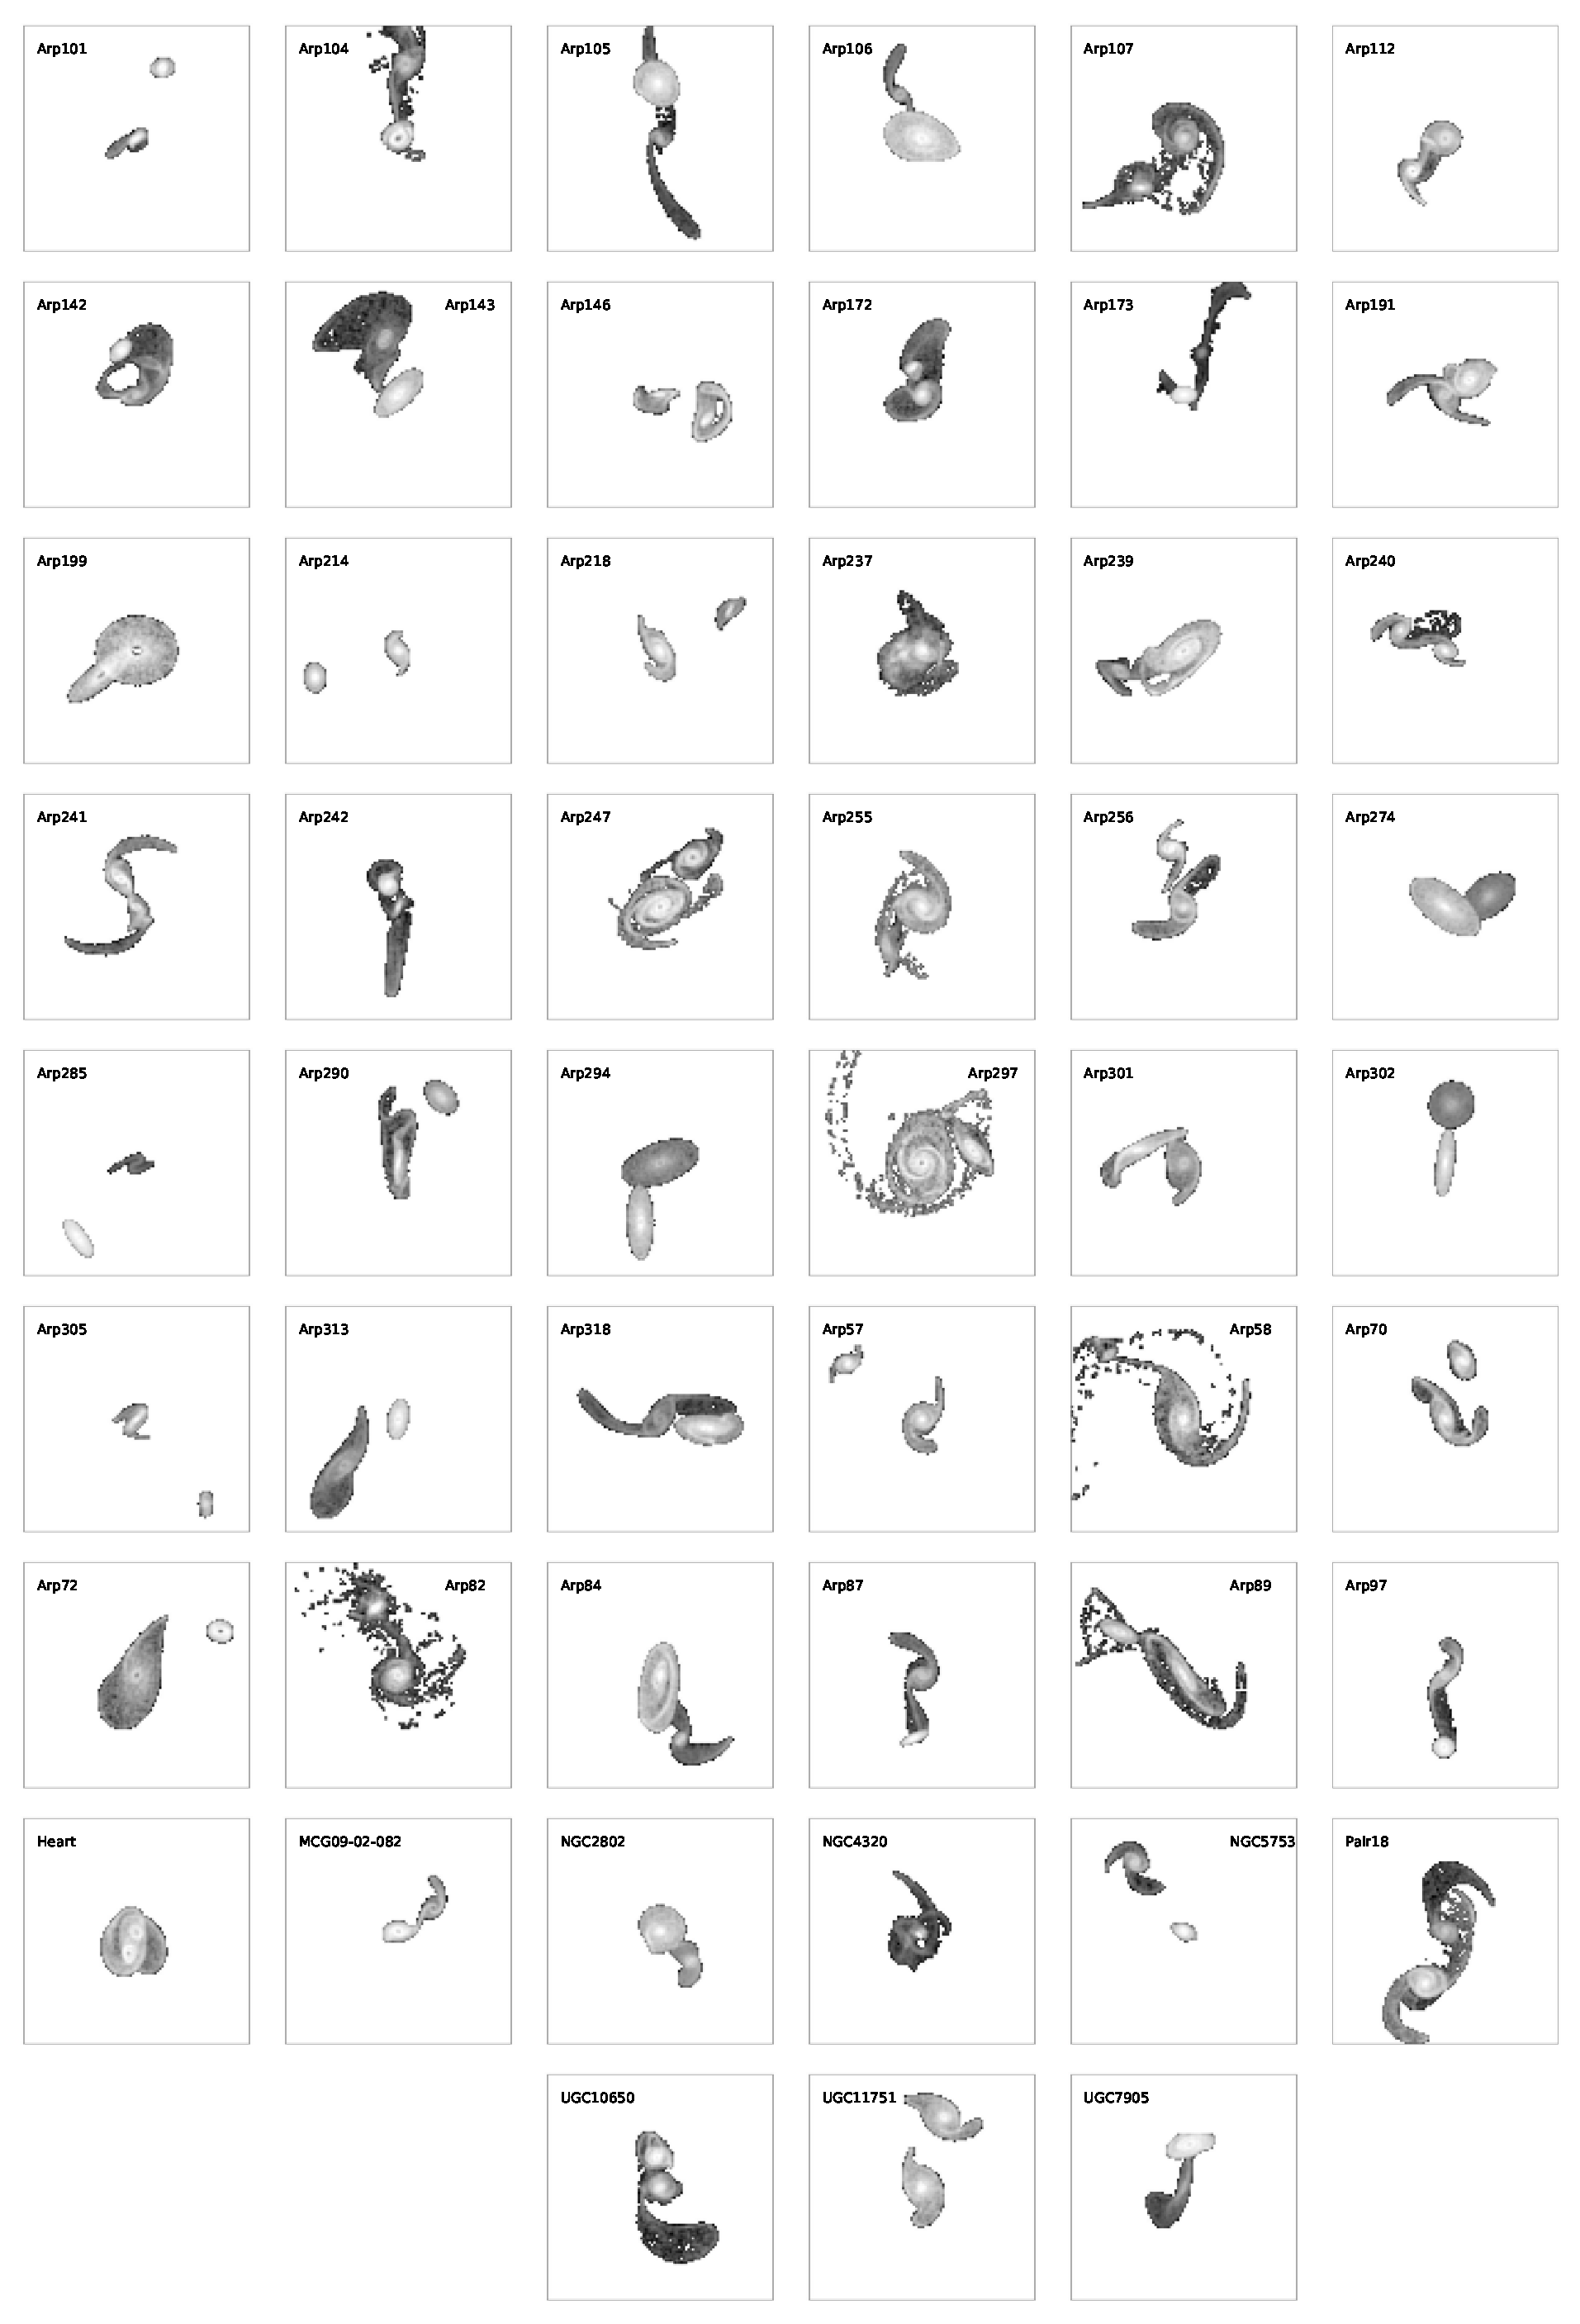
\includegraphics[width=0.90\textwidth]{Chapter1/figures/mock-images.pdf}
    \caption[Our mock observations of each interacting system.]{Our mock observations of each interacting system. These act as an idealised observation, which is completely noiseless. We also know the underlying parameters which formed these outputs. Therefore, this forms an excellent test-set to see if we can recover the underlying parameters when searching over a large parameter space.}
    \label{fig:Obj_Cutout}
\end{figure*}

\section{Constraining Interaction}\label{method:constraint}
We now require a method to compare our simulation images to our synthetic images. This comparison acts as a way to map the set of underlying parameters to an output morphology that we can then constrain by comparing to observations. However, we need a framework to conduct this comparison and to explore the parameter space of our interactions. To do this, we use an Markov-Chain Monte Carlo (MCMC) algorithm. In this section, we first describe the parameter space we explore, followed by our MCMC algorithm, how we quantify the similarity between simulation and synthetic images and how we find the parameters which are best fit.

\subsection{The Parameter Space of Interaction}
We aim to explore the underlying parameter space of interaction and find the best fit parameters which describe an input observation or test image. The parameters we constrain are the required parameters in the APySPAM three-body simulation algorithm. To function, APySPAM requires 15 different parameters. These are: the 6 positional and velocity vectors of the secondary galaxy, the total masses of both galaxies, their radius, 4 orientation parameters and the dynamical timeframe to model. We now also require the redshift measurement of the system to correctly estimate the flux distribution of the system. However, some of these parameters we can find before we begin exploring the underlying parameter space.

The first two parameters we find are the projected 2D position of the secondary from the primary. These are measured from the observational image of the system by converting between pixel and physical coordinates in the image. We take this position as the centre of the secondary disk. We also provide the redshift of the interacting system. The redshift not only directly impacts the flux distribution of the input image, but its scale and resolution. Therefore, we assume that this parameter is known and provided. Work is currently being conducted to making this a free parameter that can also be constrained based on the interacting systems flux distribution and size.

Thus, there are 13 different free parameters to recreate an interacting systems morphology and are the 13 parameters we will constrain over. A description of these parameters and the size of the parameter space explored are shown Table \ref{tab:parameters}. We choose the limits of the parameter space based on the maximum values of the parameters we used to build our test images in Table \ref{tab:Objects}. Table \ref{tab:parameters} provides the size of the parameter space as well as the conversion between the simulation units and physical units. This is primarily for reference for those who would wish to use our simulation to their own datasets. The conversions are found from \citet{1990AJ....100.1477W}.

\begin{table*}
    \centering
    \resizebox{1.00\textwidth}{!}{\begin{tabular}{|c|c|c|c|}
        \hline
        Parameter & Description & Conversion(Spec. Units) & Parameter Range(Spec. Units)  \\
        \hline
        $z$-position & Secondary $z$-position & 15kpc & -300kpc - 300kpc \\
        v$_{x}$,v$_{y}$,v$_{z}$ & Secondary velocities & 169.34kms$^{1}$ & -1693kms$^{-1}$ - 1693kms$^{-1}$ \\
        M$_{1}$,M$_{2}$ & Total Masses of Galaxy & 10$^{11}$M$_{\odot}$ & 1 $\times$ 10$^{9}$M$_{\odot}$ - 4 $\times$ 10$^{12}$M$_{\odot}$ \\
        R$_{1}$,R$_{2}$ & Radii of Galaxies & 15kpc & 0.15kpc - 150kpc\\
        $\phi_{1}$, $\phi_{2}$ & Y-axis orientation & deg & 0$^{\circ}$ - 360$^{\circ}$ \\
        $\theta_{1}$, $\theta_{2}$ & Z-axis orientation & deg & 0$^{\circ}$ - 360$^{\circ}$ \\
        t & Time of Min. Separation & 57.7Myr & 0Myr - 500Myr \\
        \hline
    \end{tabular}}
    \caption{The thirteen parameters used in both JSPAM and APySPAM to recreate an interaction. Each of these parameters must be found to consider an interaction constrained. The Parameter column shows how each parameter will be described throughout the rest of this paper. The third column then gives the conversion required to go from simulation units to SI units.}
    \label{tab:parameters}
\end{table*}

\subsection{Defining the Likelihood Function}
\subsubsection{MCMC \& Bayes Theorem}
We define framework by which to explore our parameter space, and identify areas where the parameter set successfully represent the input image. We combine APySPAM with a MCMC methodology in order to fully explore the underlying parameter space. In an MCMC, a set of walkers are created and are then moved through parameter space in an ensemble. Each walker position is a set of parameters in our 13D parameter space. At each point, we calculate the likelihood that the output simulation is representative of the input interacting system. We then compare the likelihood between the old and new position, and if the likelihood is higher at the new position the walker moves there. If not, the walker remains in place and makes another attempt to find a higher likelihood. The walkers form their own chain of steps which gradually move towards the areas of highest likelihood. In our case, the likelihood is a measurement of the similarity in flux distribution between a simulated image with parameters of the walker position and an observed image of unknown underlying parameters. Therefore, the walkers are moving from a set of underlying parameters that poorly describe the observed system to a set of underlying parameters which describe the observed system well. 

We use the well known Python package EMCEE \citep{Foreman-Mackey_13} for our MCMC. This is an ensemble MCMC package with numerous predefined moves and algorithms to make getting to the area of high likelihood more efficient. We construct contours of walker mass and use these to calculate the errors and probability distribution of our best fit measurement; i.e. we can construct a posterior for each of our parameters. For full details of EMCEE and the different modes that it can use, see the extensive readthedocs\footnote{\url{https://emcee.readthedocs.io/en/stable/}}; but here we will briefly state the hyper parameters that we use. 

For each observed image, an ensemble of six hundred walkers was initialised which would explore a total chain length of 7500 steps. Following the advice in the documentation regarding potentially complex and multi-model parameter spaces we utilised two different walker move proposals in our algorithm. These were the Differential Evolution (DE) Move \citep{Nelson_14} and the Snooker Differential Evolution (DES) Move \citep{ter_Braak_08}. An identical version of our setup can be found on GitHub\footnote{\url{https://github.com/AstroORyan}}. Here, a user can download our setup to reproduce our results, or to update the model for their own purposes.

We define a likelihood function to compare the input images to our simulation outputs. By Bayes Theorem, the probability that a set of underlying parameters which produced a simulation also describe a test image follows Equation \ref{bayes},
\begin{equation}\label{bayes}
    P(H_{i}|D_{obs},C) = P(H_{i}|C)\frac{P(D_{obs}|H_{i},C)}{P(D_{obs}|C)}).
\end{equation}
P(H$_{i}$|D$_{obs}$,C) is the probability that some hypothesised set of underlying parameters, H$_{i}$, successfully describes some observational data, D$_{obs}$, under some prior constraints, C. Applying this to our hypothesis, H$_{i}$, allows us to utilise the prior knowledge that we have about the interacting system in question and can be used to put constraints on the parameter spaces we explore to shorten computation time. This is described by the expression P(H$_{i}$|C). This is multiplied by the likelihood that the observation is defined by the hypothesised parameters given the constrains,P(D$_{obs}$|$H_{i}$,C), all divided by a normalisation constant, P(D$_{obs}$|C).

\subsubsection{Simplifying the Prior}
In order to simplify this expression, we make assumptions about the underlying parameter space to increase efficiency and simply our computations. We first assume uniform priors for each of our 13 parameters. Therefore, we define a range of parameter values that if a walker moves outwith, we set the probability immediately to zero. The ranges we allow for each parameter are specified in Table \ref{tab:parameters}. These ranges can be tweaked, or a different prior function defined, by the user. Here, we elect to set the priors part of Equation \ref{bayes} to one.

We improve efficiency in our code further by adding to the prior based on the likelihood that tidal features will form in any given interaction. This is defined by a filter parameter, $\gamma$, and is fully described in \citet[][where it is called $\beta$ but we call it $\gamma$ here to not be confused with our star formation enhancement parameter of Equation \ref{enhancement_param}]{2016MNRAS.459..720H}:
\begin{equation}\label{gamma_param}
    \gamma_{min} = \frac{M_{1} + M_{2}}{r_{min}^{2}V_{r_{min}}}.
\end{equation}
Here, $r_{min}$ is the closest approach distance, $V_{r_{min}}$ is the relative velocity at the time of closest approach and $M_{1}$ and $M_{2}$ are the primary and secondary masses, respectively. This parameter is designed to capture two important quantities: the mutual gravitational attraction and the inverse of the closest approach velocity. Each of which is important for the resultant gravitational distortion of the interacting system. By maximising the total mass of the system, while minimising the distance of closest approach and maximising the time of closest approach (i.e. minimising $V_{r_{min}}$) we would expect stronger tidal distortion. 

In our case, we use it to inform our prior as the MCMC continues. This significantly enhances the computational efficiency and pushes the walker ensemble to areas of high likelihood quickly. In each step of the MCMC, running the simulation itself is the highest computational cost, so we calculate $\gamma$ first and then make a decision on whether to run the simulation. This decision is based on an exponentially declining probability dependent on the value of $\gamma$. This probability, or prior, is defined as 
\begin{equation}\label{tidal_prob}
    C = 
    \begin{cases}
        \exp(0.5\frac{\gamma}{\gamma_{min}}), & \text{if } \gamma < 0.5 \\
        0, & \text{if } \gamma \geq 0.5
    \end{cases}
\end{equation}
Here, $\gamma$ is a user defined cutoff, 0.5 in our case. Taking the log of this, we can directly add it to prior. If the prior is initially calculated above 100, we do not run the simulation and move the walker to a new set of parameters.

\subsubsection{Simplifying the Likelihood Function}
To further simplify the likelihood function, we can assume our probability distribution is Gaussian. This is a reasonable assumption to make as a starting point for our constraining attempts. However, as will be described in section \ref{Results} this is found to not always hold true; particularly for the orientations of the system. However, making this assumption allows us to utilise the following Equation to compare our mock observations to our observed data;
\begin{equation}\label{like_gauss}
    P(D_{obs}|H_{i},C) = (2\pi\sigma^{2}_{j})\exp(-\frac{1}{2\sigma^{2}}\sum_{j=1}^{n}(x_{j}-\mu)^{2}) \times C.
\end{equation}
Here $\sigma_{j}$ is the uncertainty in the observed image, $x_{j}$ is our mock observation and $\mu$ is the observed image. The above expression can be simplified further by noting that the expression in the exponential function is just a half of the $\chi^{2}$ difference between the observational image and the mock observational image. This is the same $\chi^{2}$ function that is used in the code GALFIT \citep{2002AJ....124..266P}. Where $\chi^{2}$ is given by;
\begin{equation}\label{chi_squared}
    \chi^{2} = \frac{1}{N - n_{dof}}\sum_{0}^{N_{x}}\sum_{0}^{N_{y}}\frac{(p_{x,y} - q_{x,y})^{2}}{\sigma_{x,y}^{2}}.
\end{equation}
Here, N is the number of pixels in the observed image, which has the number of degrees of freedom subtracted from it, n$_{dof}$. $p_{x,y}$ and $q_{x,y}$ are the flux values of the (xth, yth) pixel in the observed and simulated images respectively. $\sigma_{x,y}$ is the $\sigma$ value of the (xth,yth) pixel; this is the uncertainty in the observed images pixel value and follows the $\sigma_{x,y}$-image definition from GALFIT \citep{2002AJ....124..266P,2010AJ....139.2097P}. This is then summed over all pixels in the image, giving us a single $\chi^{2}$ value between each simulated image and observed image.

Finally, to help computation time the log is taken of our likelihood function. This leaves us with a final expression that a given set of parameters describing a simulation image also describe the observed image input into the algorithm,
\begin{equation}\label{likelihood}
    \log_{10}(P(H_{i}|D_{obs},C)) = \log_{10}(L) = - \frac{\chi^{2}}{2} + \log_{10}(C).
\end{equation}
This is used at every step of our MCMC chain, with a simulation have to be run for each.

Thus, we now have a method by which to quickly predict the resultant morphology and flux distribution that the user would observe in a set of given filters. We also have a means of exploring the likely parameter space of an interaction, given an existing observation. To test this methodology, we first apply it to an idealised scenario where we know the true underlying parameters that formed the system.


\section{Results \& Discussion}\label{Results}
\noindent We now apply our MCMC algorithm to our set of synthetic interacting galaxy images. To reduce the number of repetitive figures in this paper, we focus here on a specific system as a representative sample, and publish the results of all samples online. They are presented online\footnote{All results are found here: \href{https://drive.google.com/drive/folders/1hlFhrdoZ50JaEWWYoy0RZ3J4LSoRjmsq?usp=sharing}{Link}}. As these input images are created from APySPAM, they provide us with a set of synthetic images of interacting pairs with no noise and where the underlying parameters are known. Initially, we explore the results of running this on the synthetic image of Arp 240. We discuss how the constraints could be improved, and discuss improvements on our constraints with extra, 3D information. We then plot the results for the entire dataset, and discuss trends we see in the parameters we recover.

We apply our methodology to a set of real, observed images of interacting galaxies. We select the five which are at different stages and various levels of constraint from our test dataset. We apply our MCMC to only a subset as the computational expense is significantly increased to make constraints on the observational systems and for our MCMC to reach convergence. We compare our found best fit values with those of our synthetic system, and discuss the difference between applying this to best fit simulations and observations. Finally, we describe the applicability of our approach to other systems; keeping an emphasis on those in the low surface brightness regime and the limitations this would introduce.

\subsection{Testing on a Synthetic Image}
We apply our MCMC to a single image from our mock dataset described in Section \ref{sec:syn_sample}. We elect to use this system as it is is composed of two clear and distinct disks, with a tidal bridge connecting them and tidal tails forming on the opposite side. The tidal features lie in the high surface brightness regime, and have an inclination close to 0. The observation and synthetic image are shown in Figure \ref{fig:arp240}. There are clear differences between the morphology of our mock image and the observation of Arp 240. Therefore, testing on the synthetic image is not the same as constraining the Arp 240 system. However, the synthetic image is an ideal scenario to test our methodology on. We elect to test our MCMC on the Arp 240 system first, as it has a high mass in our sample meaning the tidal features will contain more flux and should be easier for our MCMC to constrain.

\begin{figure*}
    \centering
    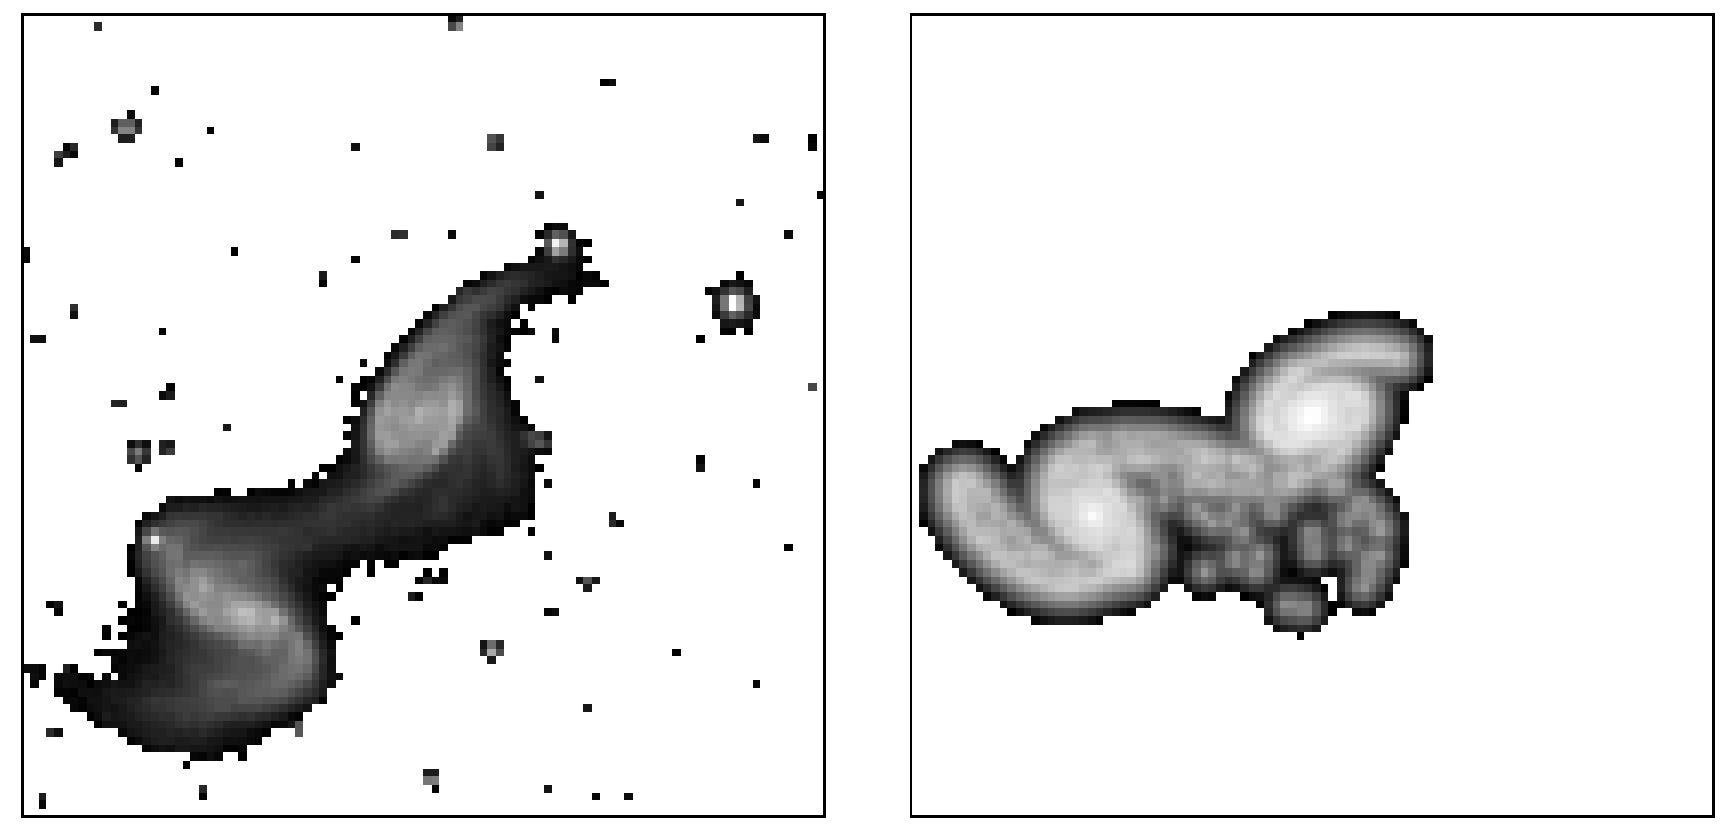
\includegraphics[width=0.75\textwidth]{Chapter1/figures/arp240-obs-sim.pdf}
    \caption[The example system used to test our MCMC: the Arp 240 interacting system.]{The example system used to test our MCMC: the Arp 240 interacting system. This system is considered an easy one to constrain. It is composed of two clearly distinct galaxies, with strong tidal features that our MCMC can match. These tidal features are the two tidal tails formed in the interaction and the tidal bridge linking the two systems. \textit{Left}: The prepared observation image of the Arp 240 system created from SDSS DR16 observations. \textit{Right}: The best fit simulation image as found by \citet{2016MNRAS.459..720H} and the first test image used in our pipeline. The different in scale and orientation are discussed below.}
    \label{fig:arp240}
\end{figure*}

We constrain the synthetic Arp 240 image by running our simulation with 2,500 particles with 600 walkers and 7,500 steps in the MCMC. An example of our full results is shown in Figure \ref{fig:corner_plot}. This corner plot is created using the Corner Python Package \citep{corner}. However, displaying our results as is shown in Figure \ref{fig:corner_plot} will be difficult as we will be discussing multiple different systems throughout this section. This larger corner plot also uses a lot of space. Therefore, we will present and discuss our results using reduced corner plots as shown in Figure \ref{fig:arp240_corner_plot}.

\begin{figure*}
    \centering
    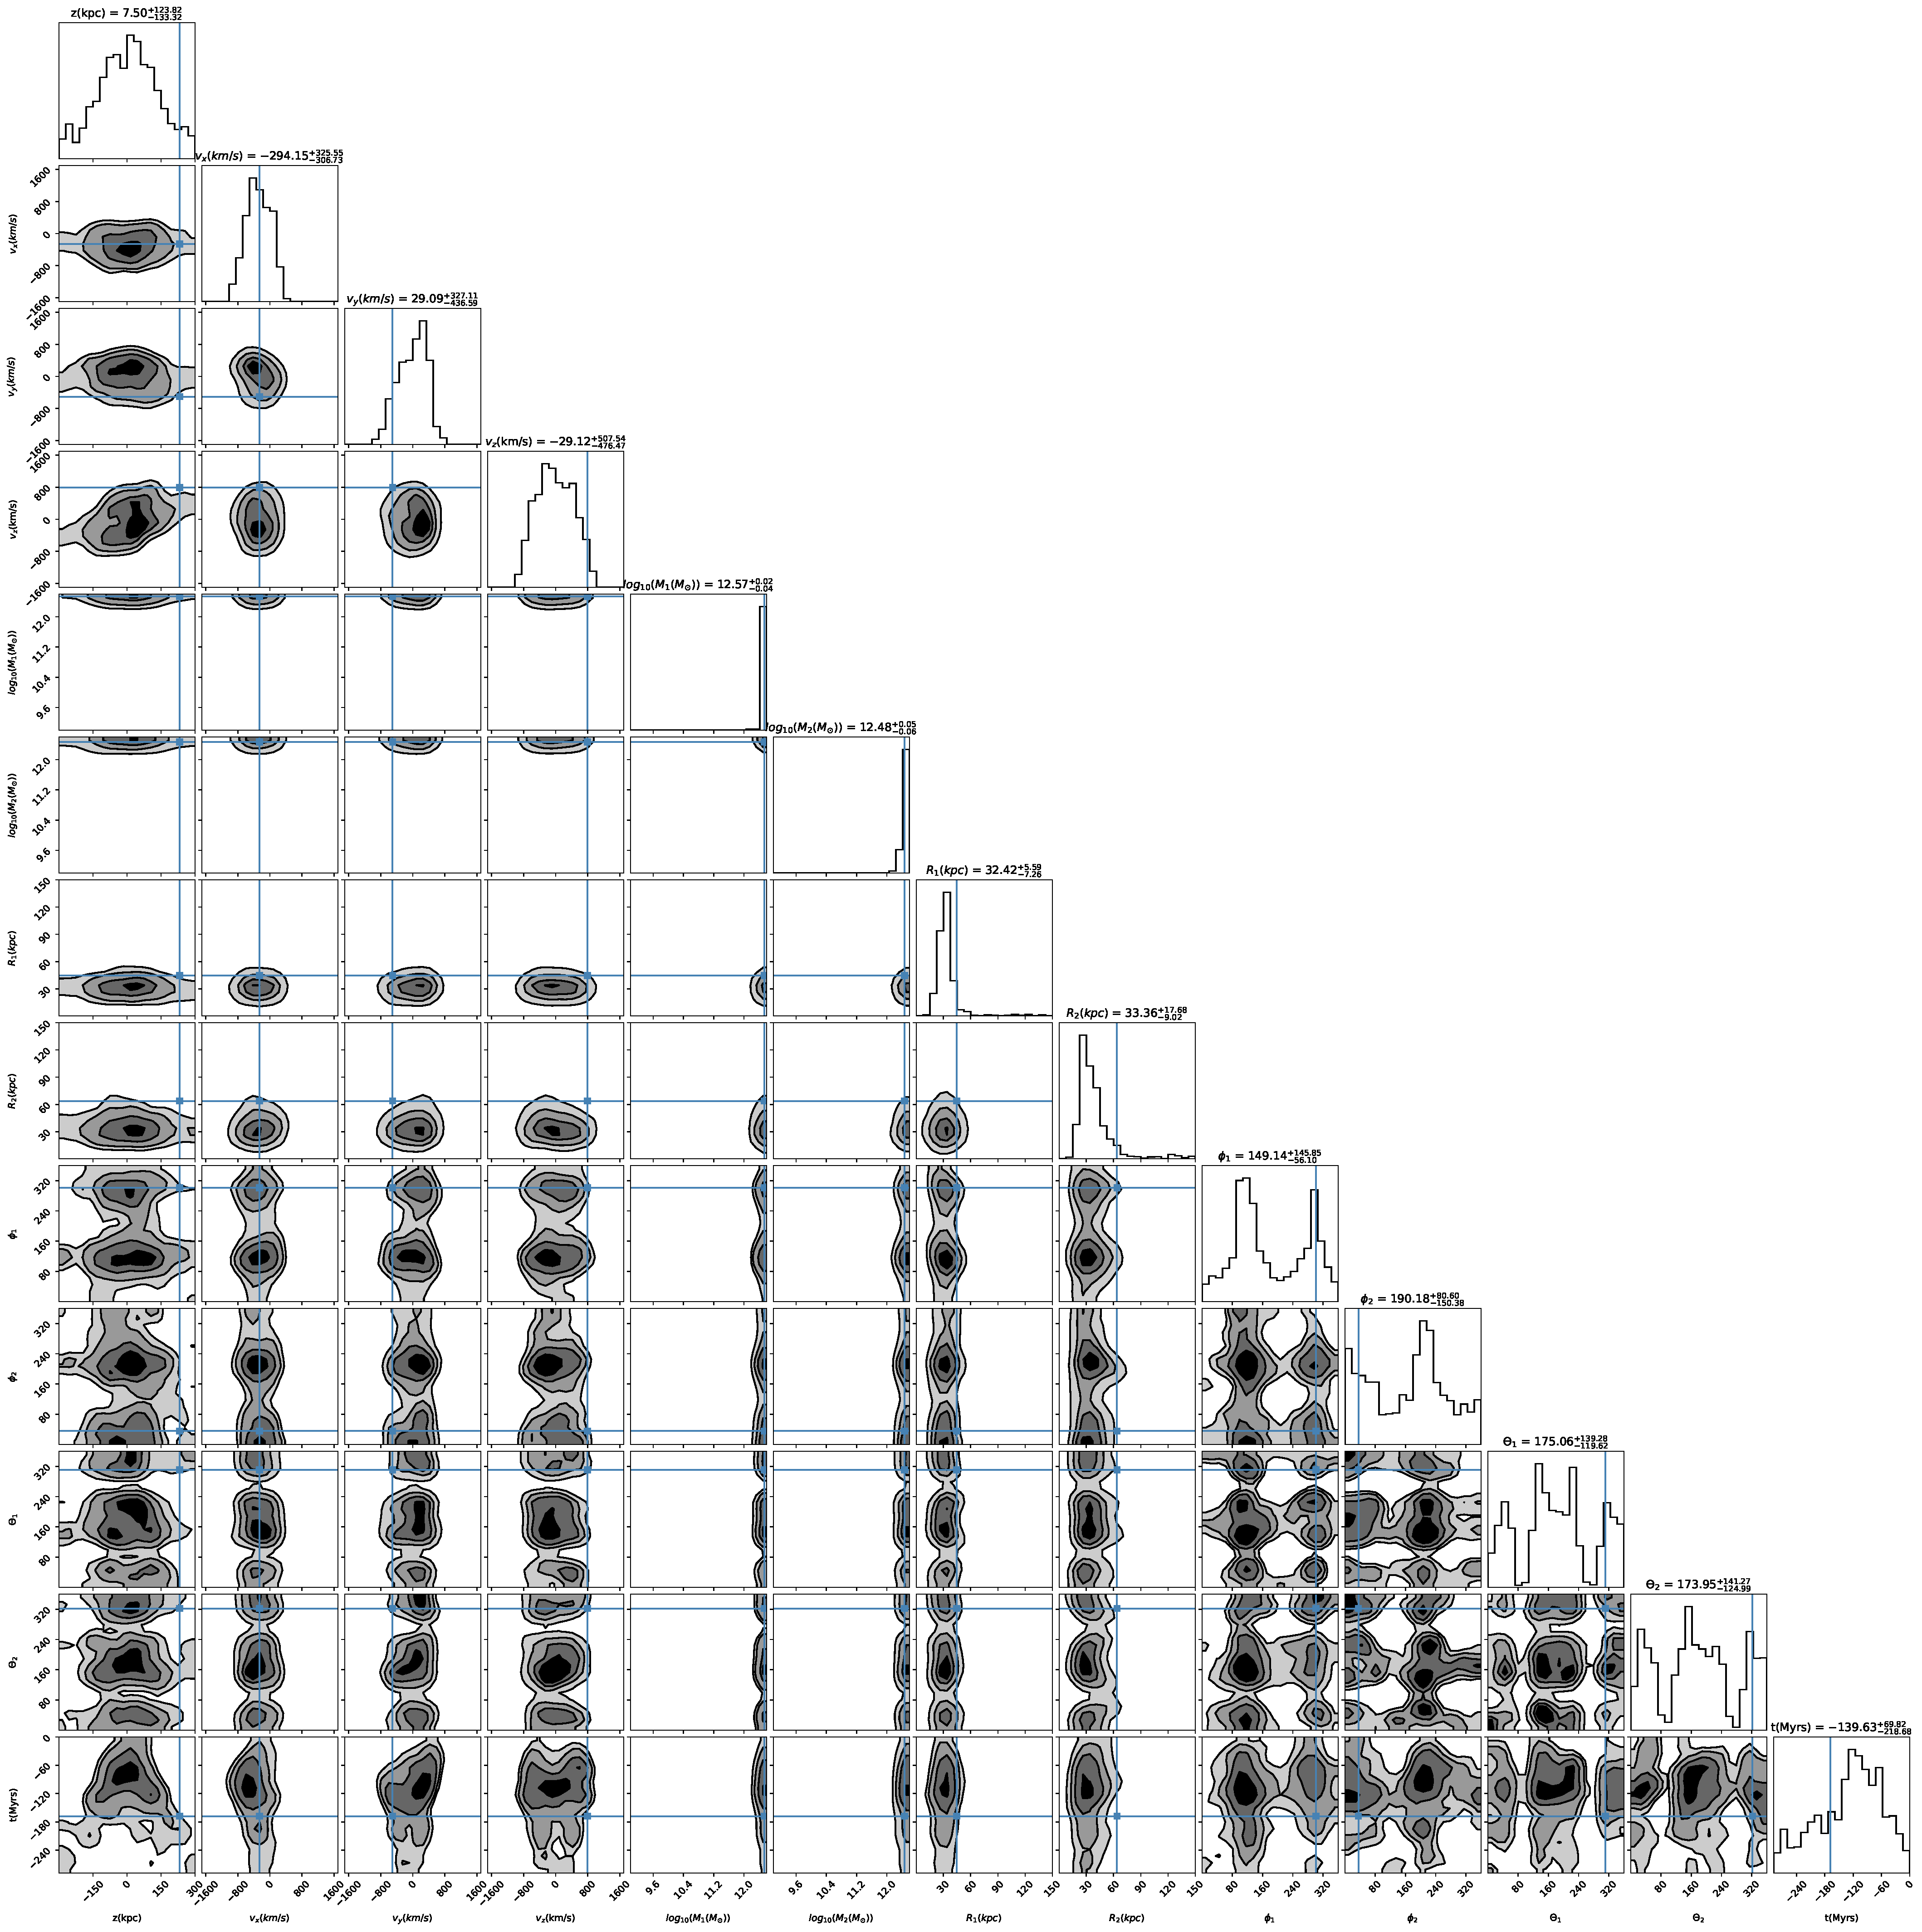
\includegraphics[width=\textwidth]{Chapter1/figures/Arp240-full-corner.pdf}
    \caption[Corner plot showing the constraints made on all thirteen parameters we are exploring.]{Corner plot showing the constraints made on all thirteen parameters we are exploring. Each contour level contains 11.8\%, 39.3\%, 67.5\% and 86.4\% of the samples across all walker chains. Displaying our results using the full corner plot is difficult in a paper because of the high dimensional results that we obtain. Therefore, we elect to show all remaining results in this paper as reduced corner plots like Figure \ref{fig:arp240_corner_plot}. We elect to put the parameters which are most likely to correlate together in different corner plots. To view the full corner plots of each system, find them at the results website for this paper.}
    \label{fig:corner_plot}
\end{figure*}

\begin{figure*}
    \centering
    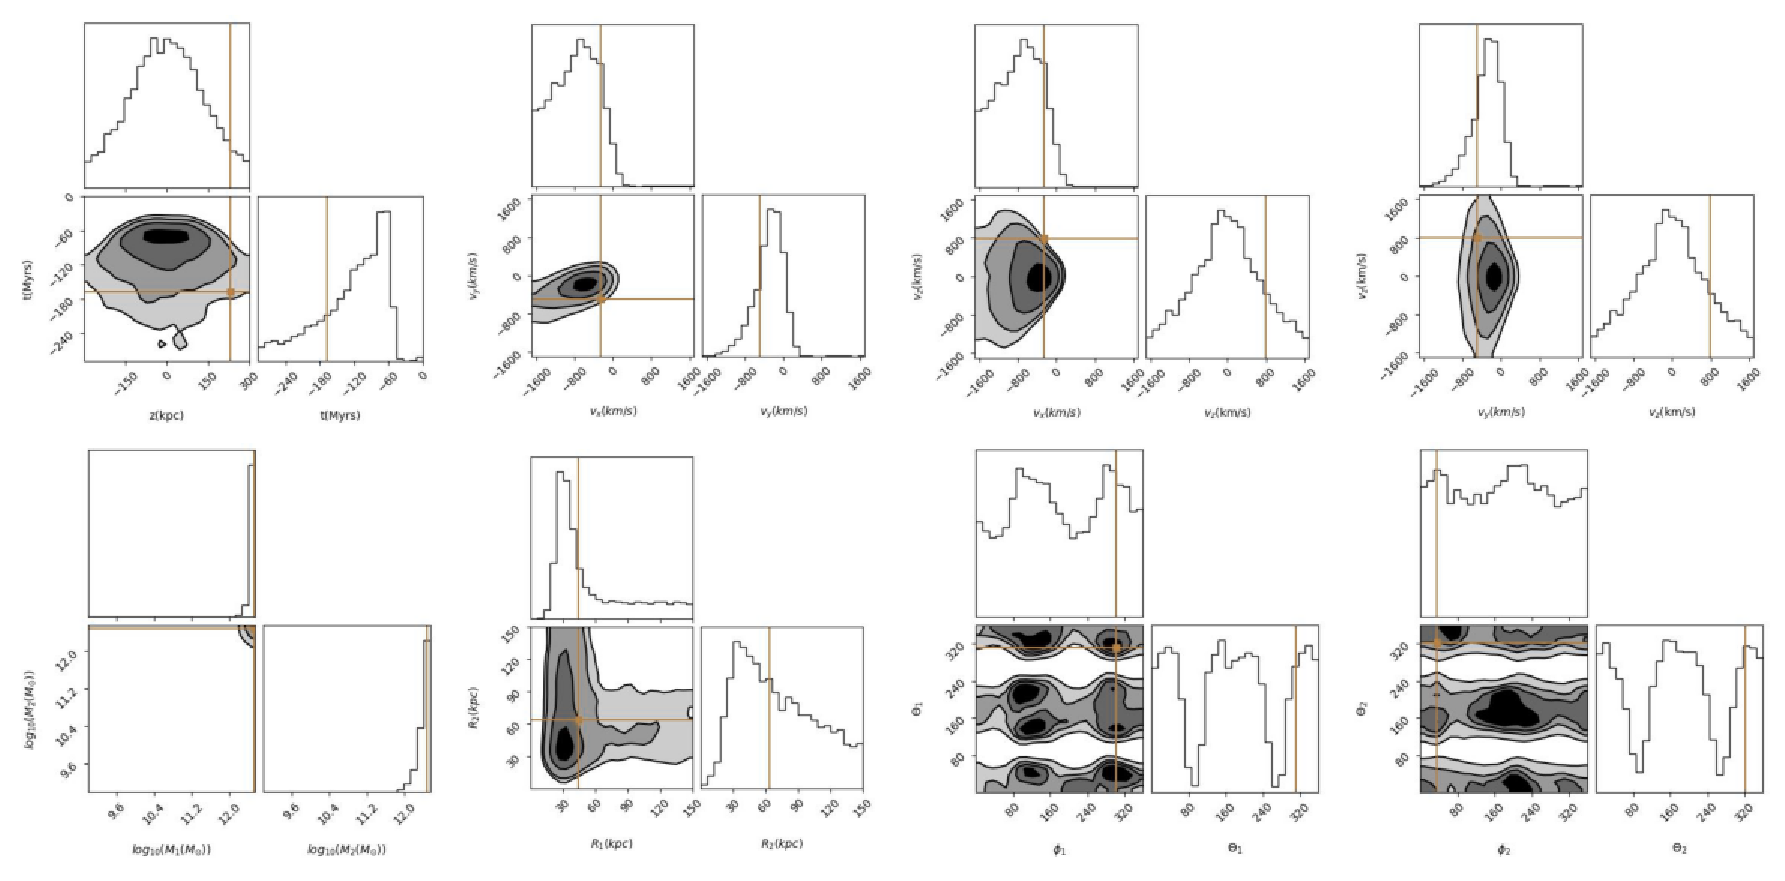
\includegraphics[width=\textwidth]{Chapter1/figures/Arp240-red-corner.pdf}
    \caption[Same as Figure \ref{fig:corner_plot}, but reduced to only corresponding parameters.]{Same as Figure \ref{fig:corner_plot}, but reduced to only corresponding parameters.}
    \label{fig:arp240_corner_plot}
\end{figure*}

% Describe the results, what are we looking at?
Figure \ref{fig:arp240_corner_plot} shows the constraints we have found on each parameter from our MCMC. The golden lines then show the true values used to create the synthetic image, and are those described in Table \ref{tab:Objects} for Arp 240. The contour levels correspond to 11.8\%, 39.3\%, 67.5\% and 86.4\% of the samples across all walker chains (these are default values), indicating the confidence level (CI). For reference, we have set up the corner plots here such that the contours containing 68\% of the walkers roughly corresponds to 1$\sigma$\footnote{Full explanation in Corner plot Docs: \url{https://corner.readthedocs.io/en/latest/pages/sigmas/}}. However, this assumes a Gaussian probability distribution, which is not strictly true for the results we find here. Figure \ref{fig:arp240_corner_plot} shows that each of the truth values is within a 67.5\% CI of the probability distribution with the exception of the $z$-position and time.

% Why do the results look like this?
We get excellent constraints on the masses of the two galaxies. This system is the most massive system in our sample, and therefore we expect the mass at the very limits of the range we are exploring. We find that the MCMC first converges on the two masses of the disks, and are the easiest for us to constrain. We provide the algorithm with the secondary 2D position, and therefore it only has to fit the flux distribution of the inner disk correctly to get good constraints on the galactic masses. The largest gains in likelihood maximisation come from matching the flux distribution in the inner parts of the primary and secondary. While the formation of the tidal features depends on the mass ratio, they also depend heavily on the orientation of the interaction as well as the relative sizes.

The relative sizes of the disks is important for the constraining the tidal features as it is the outer parts of the disk that are sheared off to form them. The primary radius is constrained very well, and is primarily expected to be smaller than the true value of this system. This is, again, due to the $\chi^{2}$ nature of calculating the distance between the two images. The likelihood, on average, is lower with some pixels within the galaxy being missed than a pixel containing the central disk in it when it should not. We therefore have a bias effect where the peak of probability drifts to just below the true value of the radius. However, the true value of the radius remains within 86.4\% CI of the found contours. 

The recovery of the radius of the secondary is worse than that of the primary. We find the peak in the probability distribution is far lower than the true value. This is from a limitation of our simulation as well. While the output simulations of the MCMC are always centred on the primary, the secondary galaxy central position is not so certain. Due to the backwards integration and trajectory calculated here, the secondary does not always end in the exact same image bin in the output simulation image. Therefore, the secondary disk likely moves slightly per simulation. This change transfers further uncertainty in the secondary disk size, and a preference for the secondary to be smaller to improve the likelihood calculation. The size of the secondary disk also contributes much more to the tidal debris formed in the interaction. The simulation is conducted in the frame of the primary, leading to the 3D velocity of the secondary being higher than that of the primary. Therefore, the particles in the secondary are much more likely to be ejected during the encounter than the simply orbiting primary particles. This adds further uncertainty to the secondary radius. However, once again, the best fit values found are within 84.6\% CI of the true value from the base simulation. 

There will also be some uncertainty involved in this measurement from the formation of the tidal features. The flux distribution of the tidal features that form are inter-dependent on multiple parameters; primarily the mass ratio, the size ratio and the orientation of the galaxies in the interaction. The significant degeneracy in the orientation constraints undoubtedly has some effect on the fitness of the resultant system. Due to a lack of three dimensional information, our algorithm cannot discern which way the galaxy is rotating or which way the tidal features should be orientated in the line-of-sight. Therefore, degeneracy at $\pm180^{\circ}$ of the true parameter values for $\phi$ and $\pm$180$^{\circ}$ for $\theta$. Figure \ref{fig:arp240_corner_plot} shows this with several different peaks in both measurements of $\phi$ and $\theta$. However, we recover the true parameters in one of the peaks of the marginalised posterior for each orientation parameter.

It is important reiterate here that $\phi$ is the orientation of the galactic disk with respect to the $y$-plane while $\theta$ is the orientation with respect to the $z$-plane. With 3-dimensional information, such as the direction of rotation of the disks or the line of sight (LOS) velocities of the tidal features, we would be able to resolve the degeneracy in the $\phi$ parameter. However, The source of the degeneracy in $\theta$ has a different source. The tidal features can form in the opposite direction from the mock observation and still be found to have high likelihood. This is a result of our likelihood being based on flux matching on pixels. There is no knowledge provided of the direction the tidal features should be moving or forming, only if the pixels contain the correct flux. Therefore, this gives a significant degeneracy in the $\theta$ parameter. Therefore, while the disk can be flipped in the $z$-direction and still match the observation, it can also be flipped in the $y$-direction as well. While the degeneracy in $\phi$ can be solved with velocity information, the $\theta$ orientation will require information on the rotation of the disk itself. Having rotational information will allow us to constrain the bulk motion within the galaxy and the direction the inner disk should be rotating as well. These two pieces of 3D information will remove the 4-fold degeneracy in each parameter.

The lack of 3D information also affects our constraints in the z-direction: the $z$-position and the $z$-velocity. As seen in Figure \ref{fig:arp240_corner_plot}, the finds the peak in the posterior distribution for both parameters as much lower than they truly are. First, the $z$-position is difficult to constrain as we lack 3D information. The simulation is run in the reference plane of the primary galaxy, therefore the secondary can only be behind or in front of iy. There will be change in the flux of the secondary based on whether it is in front or behind of the primary galaxy. However, this change in flux is completely dominated by the distance due to the redshift of the galaxy. Therefore, there is little to no observable change in the absolute values of flux unless the true value of the $z$-position was very large.

The constraint of the $z$-velocity remains far from the true parameters due to similar reasons as above. The true value lies at the very edge of the probability distribution found, at approximately 86.4\%. This would, again, be rectified readily by introducing velocity information into our constraints. The simulation works so that the secondary galaxy is always at the same x and y position that is defined by the user. Therefore, an output simulation with a positive or negative LOS velocity will have the same flux distribution. Hence, this constraint simply peaks about zero for the $z$-velocity.

Our MCMC works significantly better, however, with the $x$- and $y$-velocity of the secondary galaxy. We find the the truth value of this is within 67.8\% CI of our found distribution. The velocity values are directly related to the strength of the interaction, and therefore indirectly relate to the tidal features which form. Thus, our MCMC is informed by the flux distribution of the resultant simulated image and gives an excellent constraint on the parameters.

% Need to replace this time of interaction with the correct one. 
Finally, we discuss attempting to constrain the time of the interaction. We show the time since closest approach, not the total interaction time. The underlying simulation utilises backwards integration to calculate the trajectory of the interaction. Therefore, the time we input into the simulation simply tells it how far back in said trajectory to put the secondary galaxy. Therefore, the same interaction will occur whether we input -10 time units or -100 time units. The algorithm will require more computation time to calculate the particle positions in the lead up to the interaction. It is important to note that the total integration time will only affect the output system when we make it too small. In other words, if the secondary starts after the point of closest separation or at closest separation, our simulation breaks down and gives nonphysical results.

We calculate the time of closest approach for all of our walker steps and then present this as a measure of the time posterior distribution. Our measured value is significantly smaller than the true value of our best fit simulation, although it does lie within the region of 86.4\% CI. This parameter is highly dependent on the velocity and position constraints that we have made, and these are skewed to significantly smaller values than the truth. Therefore, it is unsurprising that our time of closest approach value is also found to be much smaller.

To fully put this result into context, we explore the simulations that lie in the areas of highest probability within these posteriors. To select which simulations to present, we take those walkers that were within the 11.8\% CI throughout each walker chain and take the top 5 as an illustration here. Our MCMC is not able to precisely reproduce the input image. It is often able to reproduce the tidal features of the primary as well as the tidal bridge connecting the two systems. This appears to be where the MCMC has centered the posterior upon. The likely reason for this is actually due to the filtering parameter that we use on the simulation. The Arp 240 simulation lies in an unlikely area of tidal features to form - $\gamma = 0.259$ - and, therefore, we update our prior to make the true result appear less likely. However, the $\gamma$ parameter remains a necessity in our MCMC. Without the ability to filter the simulations quickly, we begin to approach very large requirements of computational expense. Therefore, for this particular example the $\gamma$ parameter is a hindrance.

\begin{figure*}
    \centering
    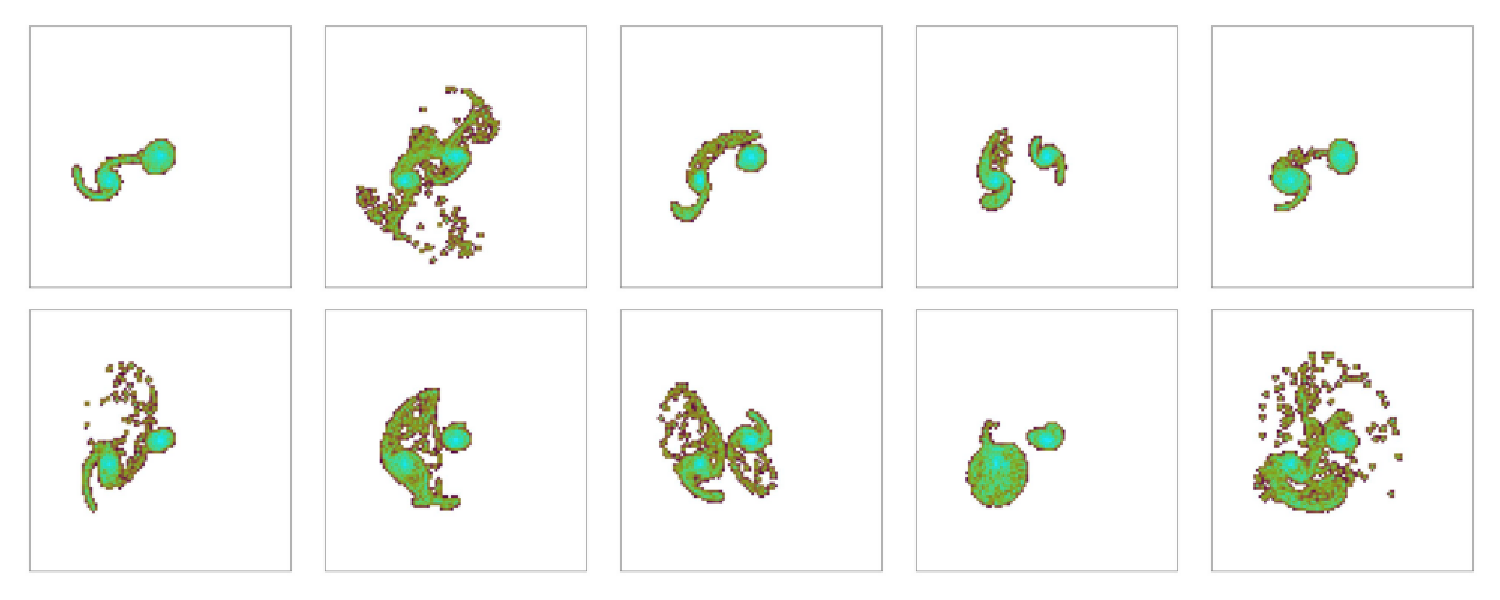
\includegraphics[width=\textwidth]{Chapter1/figures/best-fits-comb.pdf}
    \caption[Simulations from the areas of parameter space that lay within the 11.8\% CI of our constraints.]{Simulations from the areas of parameter space that lay within the 11.8\% CI of our constraints. \textit{First Row}: The synthetic image we are attempting to constrain. \textit{Second Row}: The best fit simulations from this parameter space. \textit{Bottom}: The worst fit simulations from this parameter space. Our MCMC found those parameters which cause the formation of the correct tidal features, as well as the tidal bridge connecting the two systems. However, it has been unable to fully identify the tidal features of the secondary. There is also a lot of noise in this posterior distribution, with many systems with different tidal features in the areas of high probability. Therefore, identifying specific systems with the sought after tidal features requires manual intervention.}
    \label{fig:arp240_corner_plot}
\end{figure*}

% This is likely better in the conclusion.
In the surrounding area of probability space, however, we find some interesting constraints. Changing each parameter by small amounts based on the posteriors of each parameter space leads to variation in the simulation outputs and tidal features. Due to the disks being well defined and aligned, this can often lead to them being weighted highly. Therefore, the question remains, how would one use this code to find their best fit simulation and actually make constraints using it? This algorithm is best used as an indication of where in parameter space the true parameters lie in recreating the tidal features observed in an observation. This reduces the size of parameter space to explore dramatically, and could be an indication of where to search with more accurate simulation models for true interacting galaxy parameters.

Overall, from our example of Arp 240, we are able to recover nearly all the true values of the input simulation to within an 86.4\% CI of the true parameters. The only missing parameter is the time since the flyby. There is significant degeneracy in constraining the orientations of this interaction, but this is expected. While our results appear like they have converged in the MCMC, we will also describe the diagnostics with which to prove this. 

\subsection{Diagnostics of Pipeline}
% Note, a quick section to discuss the diagnostics of the pipeline, proved it's converged etc. If I cannot get Chain Consumer working here, then I won't do this section.
\noindent It is important to ensure our results are reliable by using diagnostics to investigate the MCMC chains. We investigate three different diagnostics of our MCMC run. First, we check that they have truly converged with the Geweke diagnostic. The Geweke diagnostic is a Z-test of equality of means where the autocorrelation in the flattened samples is taken into account as the standard error is measured. We compare the means of the first 10\% and last 50\% of each chain in each parameter, and require the resultant Z-score to be $<1$ for convergence. We use the Geweke diagnostic as written in the ChainConsumer \citep{2016JOSS....1...45H} Python package. For this case, every parameter passes this convergence test, with the exception of the orientation parameters (although, this is likely the result of converging on multiple best-fit values).

Figure \ref{fig:arp240_corner_plot} clearly shows that each orientation has incredibly complex, multi-model structure in the parameter space. We have a 2- or 4-fold degeneracy in the output models due to three dimensional information not being available. This disrupts our Gewke diagnostic measure, which is looking for a single peak in parameter space. Therefore, by folding the parameter space over and only exploring over $0^{\circ}$ - $180^{\circ}$, we achieve a single peak in parameter space. These results then pass the Geweke diagnostic test.

\begin{figure}
    \centering
    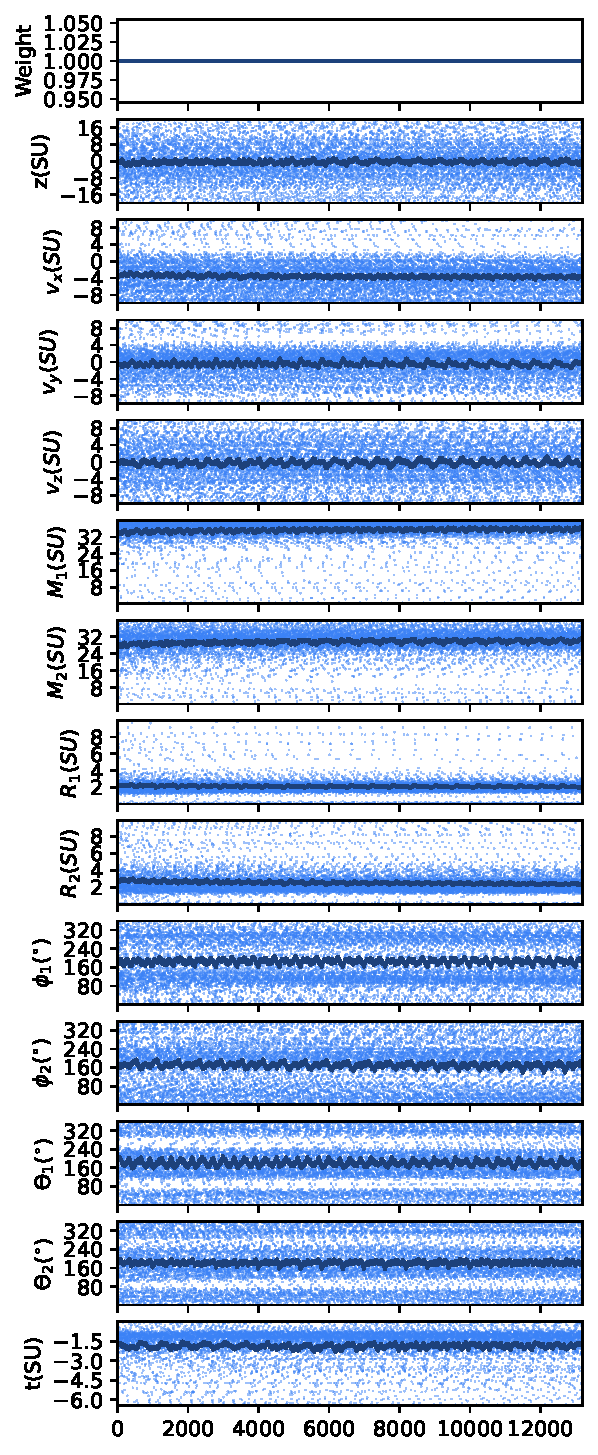
\includegraphics[width=0.45\textwidth]{Chapter1/figures/arp-240-steps.pdf}
    \caption[Steps taken by each walker in our MCMC chain to constrain the Arp 240 best fit simulation.]{Steps taken by each walker in our MCMC chain to constrain the Arp 240 best fit simulation. Note, the $y$-scales here do not extend over the full parmaeter space for some galaxies, and only show where the walkers have stepped after the burn-in phase. The deeper the blue, the more walkers have stepped at that point. This figure shows that our MCMC has successfully burnt in and very quickly goes to high areas of probability for parameter space. They then oscillate around the best fit values while searching the remaining parameter space. The $z$-position, $z$-velocity and $\phi_{2}$ parameters show dignificant uncertainty as the walkers move around the entire parameter space. In the $\phi_{1}, \theta_{1}, \theta_{2}$, we can see the two fold degeneracy form very early on and then the walkers do not explore across them at any point.}
    \label{fig:walker_steps}
\end{figure}

The second diagnostic we use is that the walkers have fully explored parameter space and that we have removed enough of the steps at the beginning of the run to consider the MCMC burnt-in. Once again, using ChainConsumer, we can plot out each walker step throughout parameter space. Figure \ref{fig:walker_steps} shows the flattened walker chains through parameter space. We have removed the first 200 steps of each walker chain before thinning the chain and flattening it. By flattening we have taken each walker chain and combined them into one chain for every parameter. Discarding the first 200 steps has been enough for the burn in of the MCMC, as the walkers have already moved mostly through parameter space and are centering on a central value of high probability. The structure in the orientation parameters is also interesting. The degeneracy structure in the parameter space has already formed by the end of the burn-in and then the walkers move within those areas of high probability. This is for two reasons. First, they affect the flux distribution of the disks primarily in if they are face-on or edge-on. The MCMC quickly converges on face-on systems in our case. Second, when they are in that degenerate space, the slight changes in inclination of the disks given does not change the likelihood calculation significantly enough to reduce this degenerate space further. Hence, the degenerate areas are very large with very flat areas of probability at their peak.

We have tested resolving this problem by running further steps in our MCMC to achieve convergence naturally within the parameter space. We find that increasing the number of steps does improve convergence on the orientation parameters, but at a much larger computational cost and without substantial improvement on the other parameters. Therefore, we elect to fold our resultant degenerate solutions into a smaller parameter space. This achieves convergence, and gives us excellent estimates on the orientation for these systems.

A second solution to this problem would be involving velocity information into our models. Knowing the bulk motion of the tidal features would allow us to constrain the tidal features based on which way they were rotating. This would eliminate part of the degenerate space. However, as stated previously, little spectroscopic data exists of our sample of interacting galaxies. Therefore, we run this test using the our synthetic Arp 240 image and including the LOS velocity of the particles and creating a velocity grid to constrain over.

\subsection{Inputting 3D Information}
Very few of the systems described in Table \ref{tab:Objects} have associated integral field spectroscopy (IFU) data in order to get LOS velocities to incorporate 3D information into our fitting process. This is because they are very large in the field-of-view of many instruments, and therefore we can only achieve measurements of their inner disks and not their tidal features. We, therefore, map the velocity distribution of our synthetic Arp 240 image. This map is created by summing the $z$-velocities of each particle in the bin and then create a total LOS velocity map for which to compare to simulations. This has little impact on the measurements of mass, size and $x$- and $y$-velocity measurements. However, it completely changes our measurements of the $z$-position and time of interaction as well as improves our constraints on all three velocity vectors dramatically. 

Figure \ref{fig:velocity_corner_plot} shows the new measurements of the constraint on the $z$-position, $y$- and $z$- velocities. The constraints on each of these parameters is significantly improved. This is with the same number of MCMC walkers and steps as without 3D information. For the $y$- and $z$-velocities, the constraints are improved to the point where we completely recover the true underlying parameter values within 39.3\% CI. With the $z$-position, we also gain significant constraint. We are able to recover which side of the primary the secondary lies, with a sharp drop in the marginalised posterior over the negative part of the $z$-position parameter space. We also significantly improve our constraint on the time of the interaction, and approximately recover the true parameter. We are able to constrain the final velocity expected in the observation, and therefore, means the galaxy cannot be moving too fast at in the final timestep. This has the effect of shifting the expected time of contact back significantly.

\begin{figure*}
    \centering
    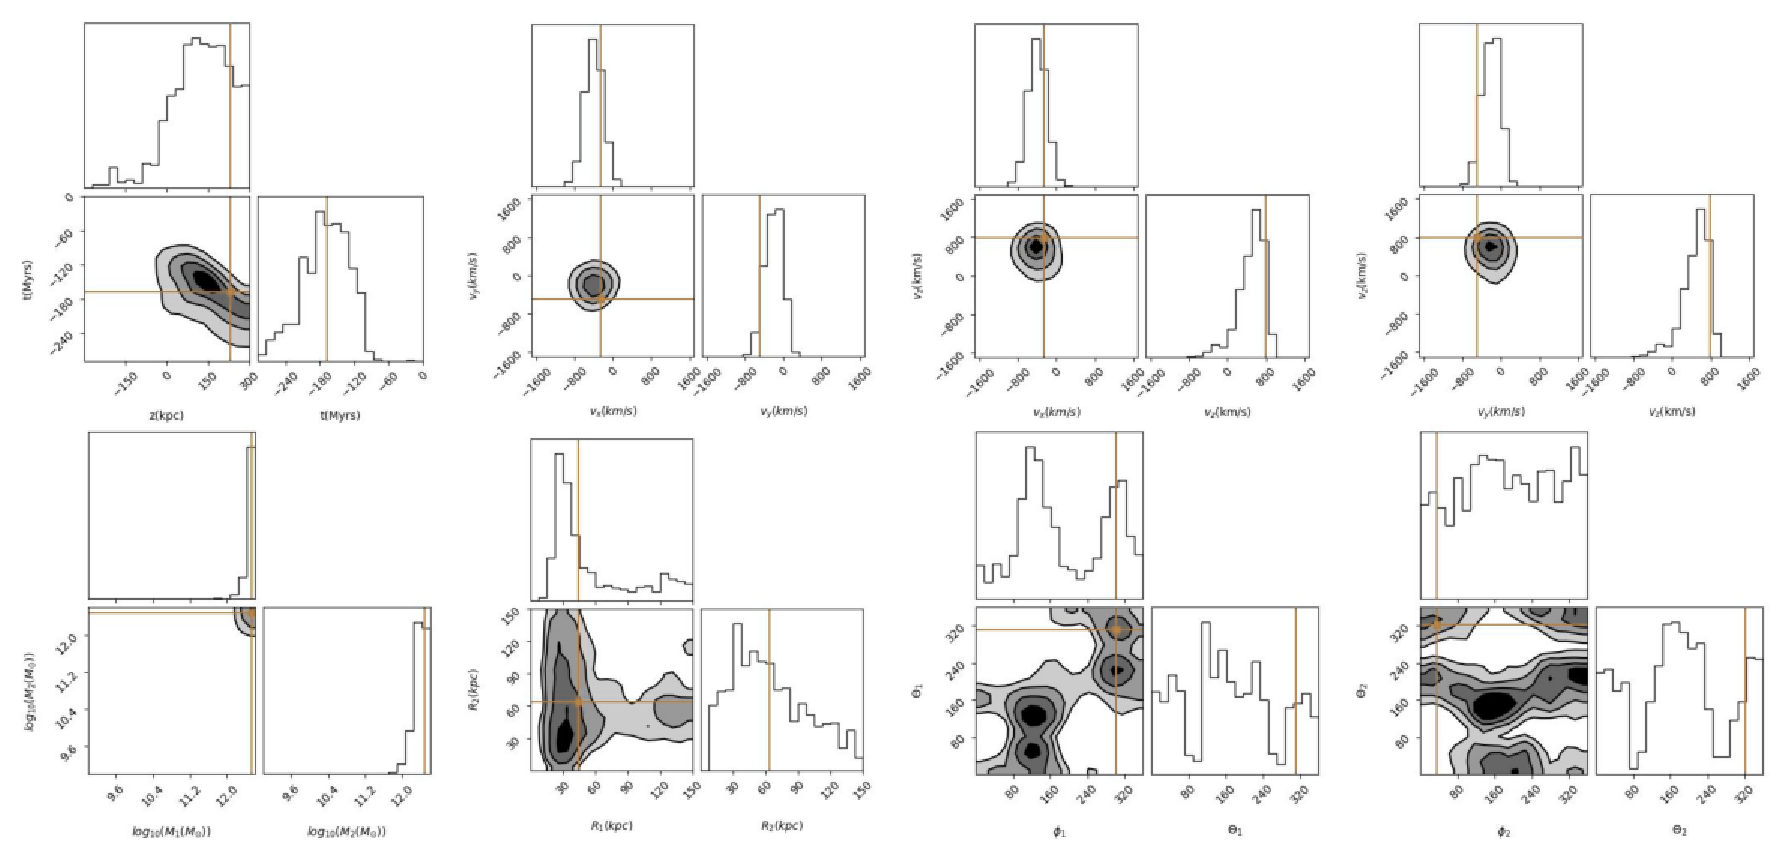
\includegraphics[width=0.9\textwidth]{Chapter1/figures/Arp240_vel-red-corner.pdf}
    \caption[The reduced corner plot of the synthetic Arp 240 system with a velocity map also used for constrained.]{The reduced corner plot of the synthetic Arp 240 system with a velocity map also used for constrained. To add this extra information, we created a mock velocity map of our Arp 240 synthetic image and summed the LOS velocity ($z$-velocity) in each pixel of our image. Comparing between here and Figure \ref{fig:arp240_corner_plot}, we see we make different constraints on the $z$-position and the time as well as resolve one of the degeneracys in the orientation space.}
    \label{fig:velocity_corner_plot}
\end{figure*}

Interestingly, we lose a significant amount of constraint on the relative sizes of the two systems. Adding the velocity information in the way we have likely increases the required size of the disks so the LOS velocities match within them. Therefore, more particles are stripped from the secondary galaxy and cause further uncertainty in the final image. We also find the removal of some of the degeneracy in the orientation parameters, as expected. It is important to note that, in this example, we have only used the LOS velocities to achieve this improvement in constraint. To better get constraint on orientation, we likely need further velocity and 3D information of the system. For instance estimates of the internal rotation, and accurate measures of the bulk motion of the tidal features in the galaxy. Currently, the simulation is not able to accurately reproduce this outwith simply assuming circular velocities at different radii from each galactic centre. Finally, the mass constraints remain the same as was found without velocity information as they are dependent primarily on the flux distribution and dominated by the inner disk of the system.


This shows the improvement that adding velocity information to our MCMC could bring, and how far interacting galaxy simulation and constraint can go once we incorporate IFU spectroscopy over more systems. In the sample we are using here, of the most massive, large, major interacting systems, only three have got any IFU data. This data is from the MaNGA \citep{2015ApJ...798....7B} IFU spectrograph, whose field of view is only able to capture the central disk of these systems. While having velocity information on even a subset of the pixels of the galaxy would improve constraints, to significantly improve them we will need this of the full tidal features of the systems. IFUs with larger fields of view are soon to come online, such as WEAVE \citep{2014SPIE.9147E..0LD}. 

\subsection{Running on Full Idealised Sample}
% Remember, this section is meant to be an overview of all of the results and simply a discussion on what we notice of applying it to different systems. This is not another deep dive like we did in the testing on one system. 
\noindent With constraints being ascertained on nearly all parameters of our synthetic Arp 240 image, we then applied our MCMC to the remaining 50 synthetic images. The reader is invited to see the resultant corner and reduced corner plots of each system on the website. Here, we will detail describe our best and worst three corner plots, and then discuss the trends throughout applying the MCMC to the dataset. First, our ability to constrain is highly dependent upon the stage of interaction. Our tightest constraints, the ones with narrowest posteriors, were on those interacting galaxies which were only just past the point of closest approach. I.e., they were the systems which had highly distinct tidal features and disks were fully separate. Our best three fits were those of synthetic images of Arp 172, Arp 240 and Arp 290. The `best fits' have been judged by those with the smallest FWHM of their marginalised probability distribution in mass. The reduced corner plots are shown in here in Figures \ref{fig:arp240_corner_plot}, \ref{fig:best-Arp172} and \ref{fig:best-Arp290}. Each of these systems is clearly in stage 2 or 3 of the interaction, where tidal features have formed clearly, and there are two distinct disks.

\begin{figure*}
    \centering
    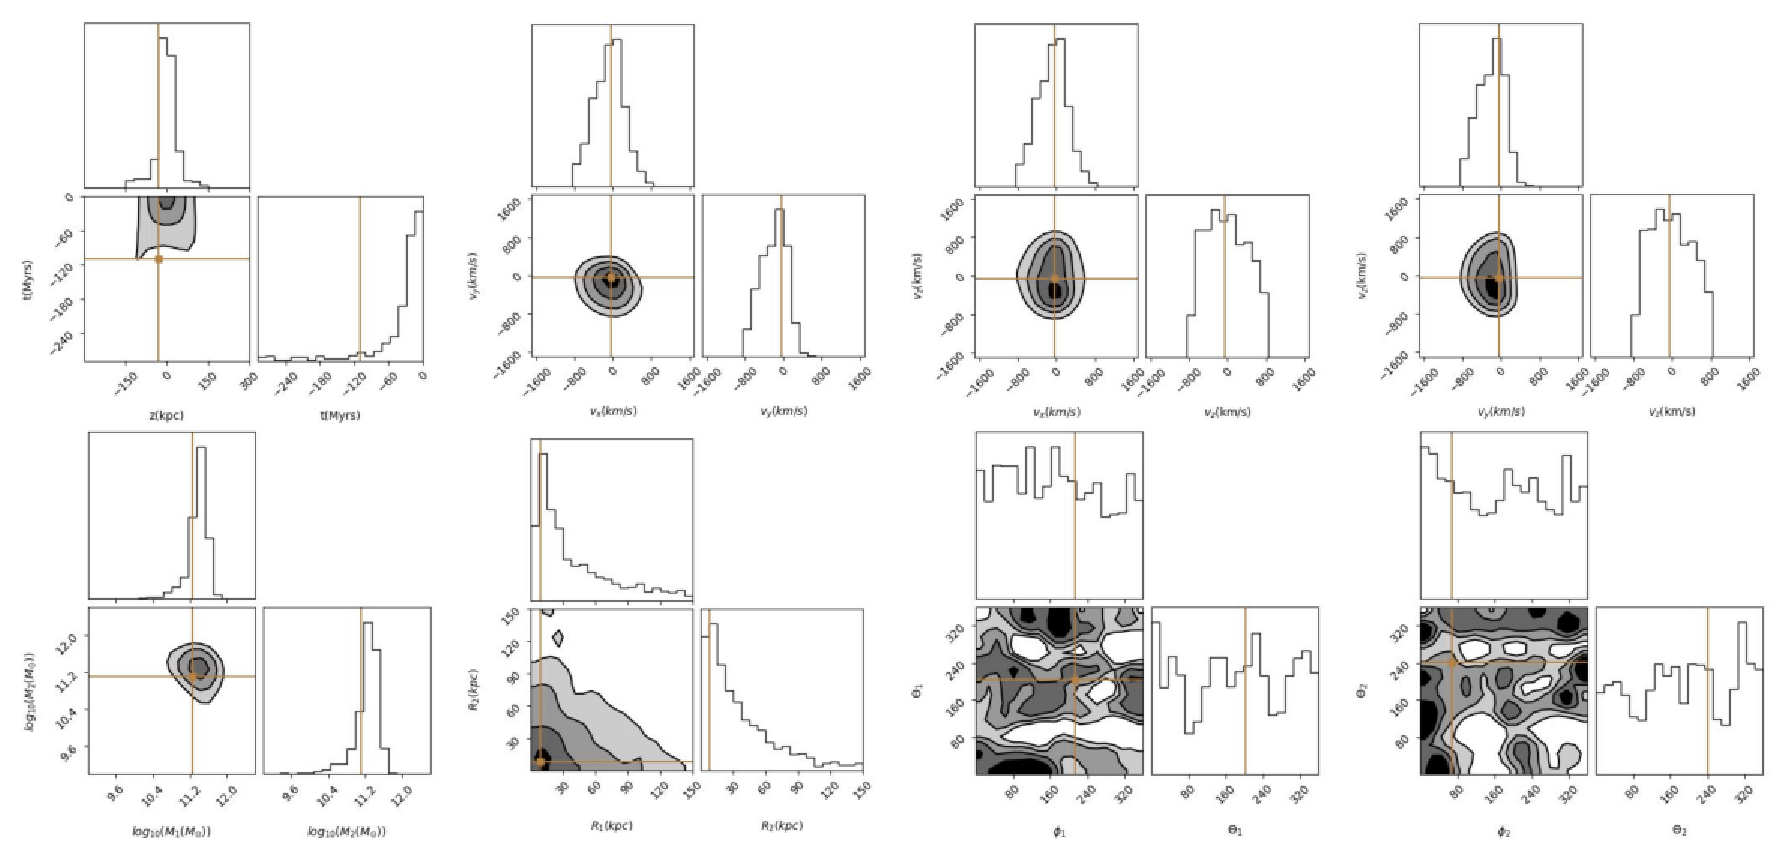
\includegraphics[width=\textwidth]{Chapter1/figures/Arp172-red-corner.pdf}
    \caption[Second example of our best fits from our methodology is representative of the simulated image of Arp 172, a stage 3 system.]{Second example of our best fits from our methodology is representative of the simulated image of Arp 172, a stage 3 system. Gold lines represent the true values.}
    \label{fig:best-Arp172}
\end{figure*}

\begin{figure*}
    \centering
    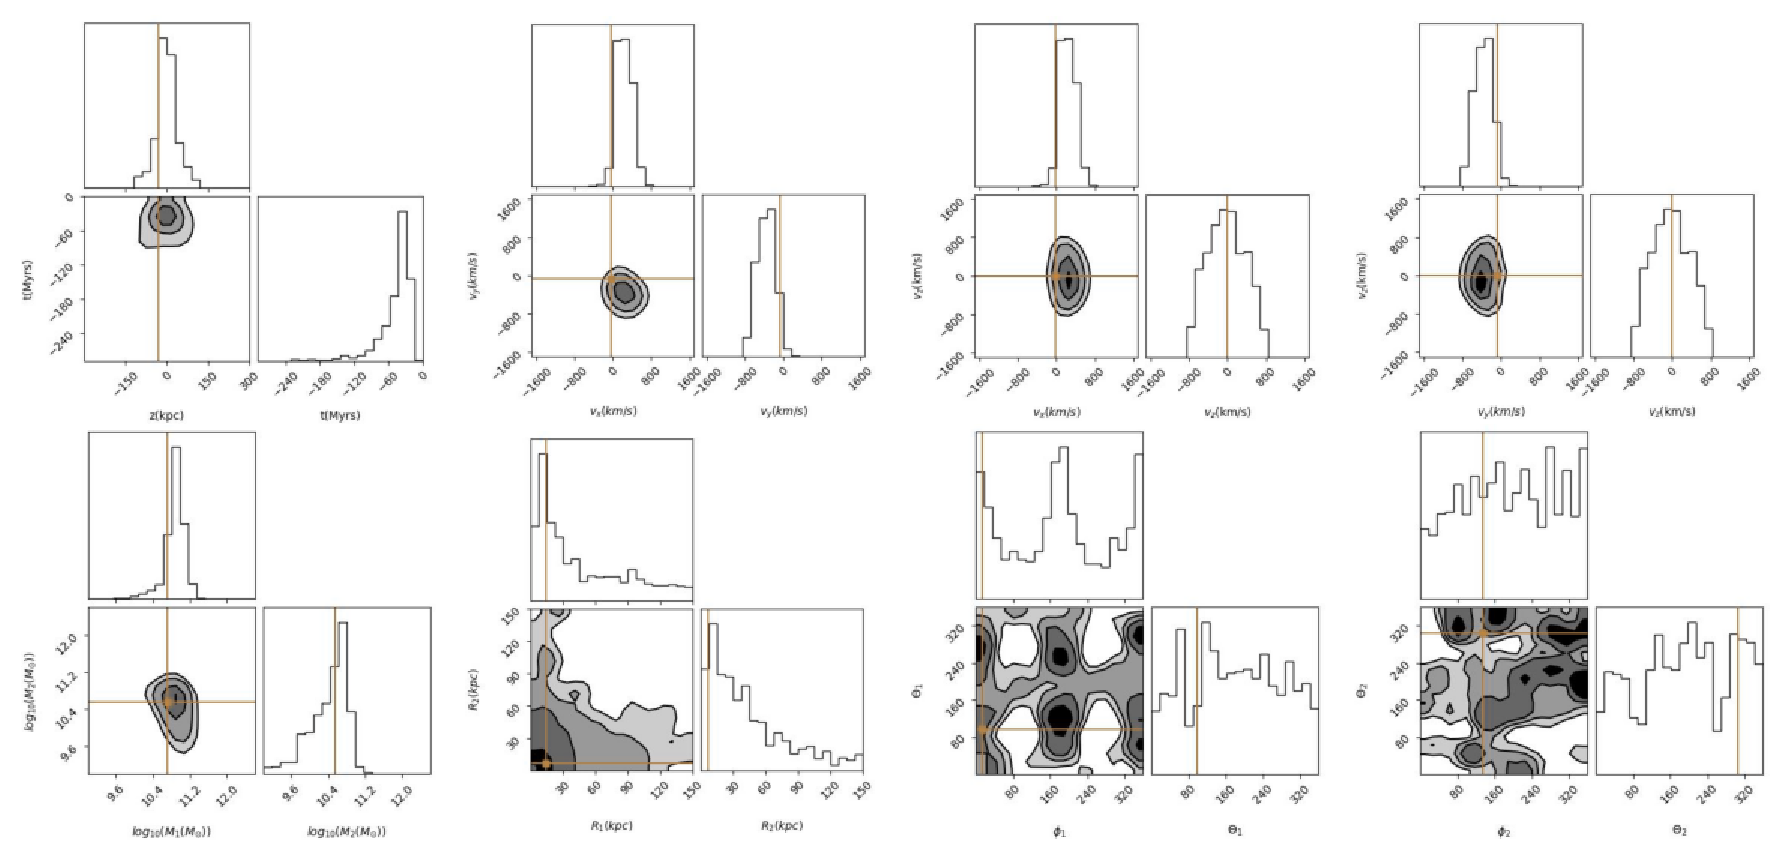
\includegraphics[width=\textwidth]{Chapter1/figures/Arp290-red-corner.pdf}
    \caption[Third example of our best fits from our methodology is representative of the simulated image of Arp 290, a stage 2 system.]{Third example of our best fits from our methodology is representative of the simulated image of Arp 290, a stage 2 system.}
    \label{fig:best-Arp290}
\end{figure*}

\begin{figure*}
    \centering
    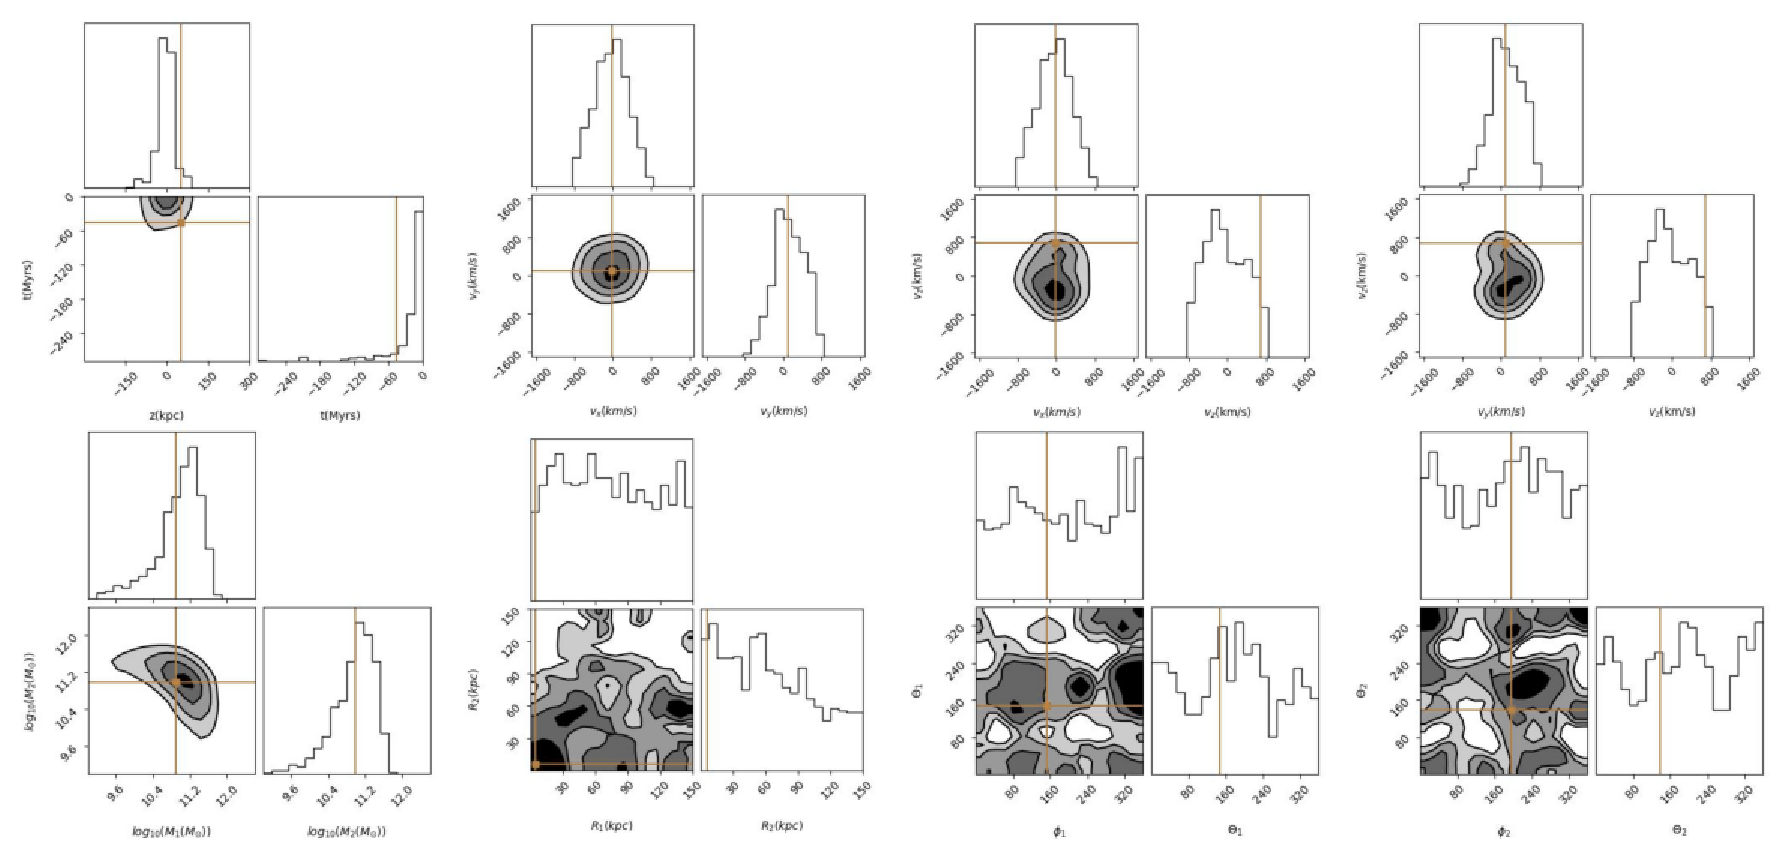
\includegraphics[width=\textwidth]{Chapter1/figures/Heart-red-corner.pdf}
    \caption[First example of our worst fits.]{First example of our worst fits. This shows our constraints of the simulated image of the Heart system, a stage 4 system.}
    \label{fig:worst-Heart}
\end{figure*}

\begin{figure*}
    \centering
    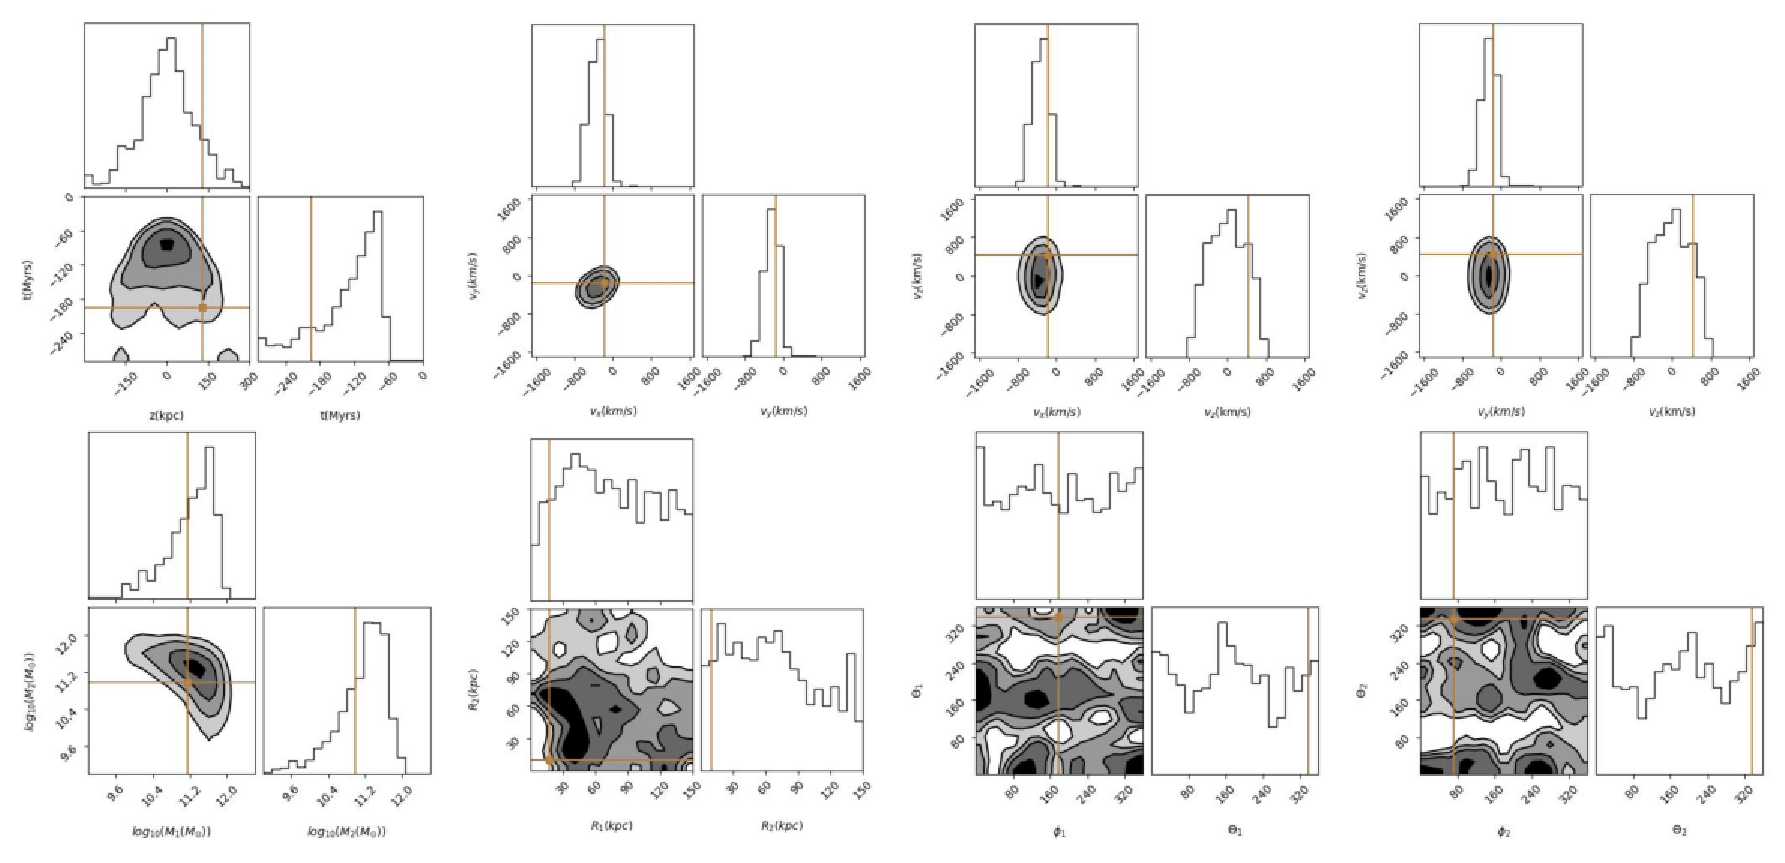
\includegraphics[width=\textwidth]{Chapter1/figures/Arp57-red-corner.pdf}
    \caption[Second example of our worst fits.]{Second example of our worst fits. This shows our constraints on the simulated image of NGC 4320, a stage 4 system.}
    \label{fig:worst-Arp57}
\end{figure*}

\begin{figure*}
    \centering
    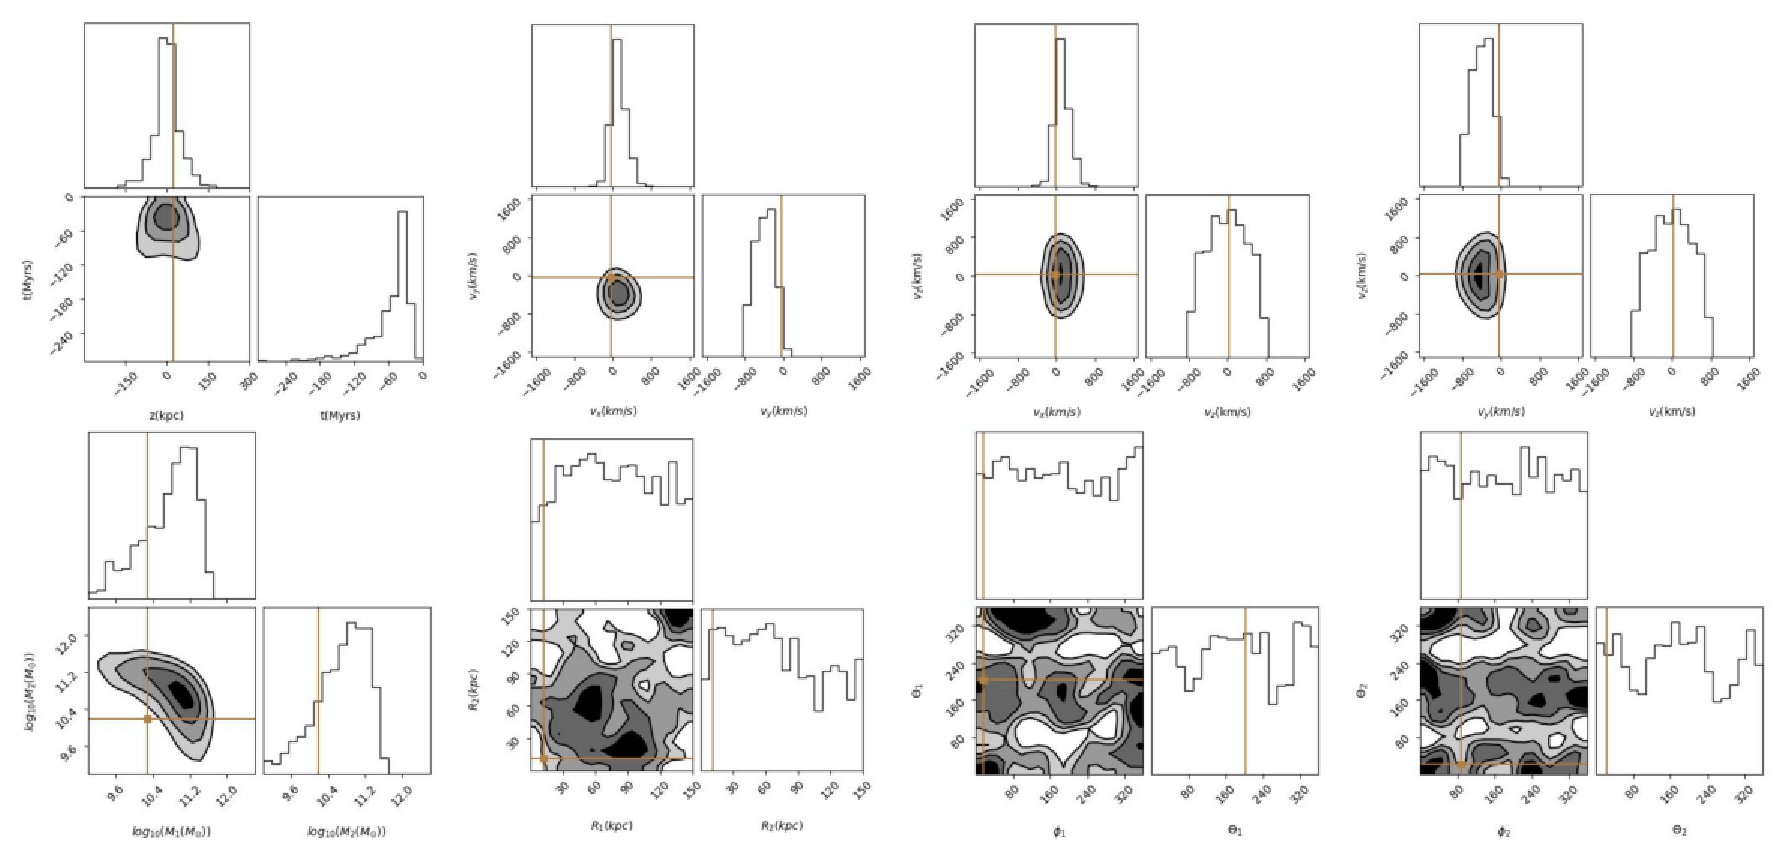
\includegraphics[width=\textwidth]{Chapter1/figures/UGC11751-red-corner.pdf}
    \caption[Third example of our worst fits.]{Third example of our worst fits. This shows our constraints on the simulated image of UGC 11751, a stage 3 system.}
    \label{fig:worst-UGC11751}
\end{figure*}

The worst fits we achieved were of those systems which were close to the merging stage. They were systems where the two cores were close to coalescence, very little tidal features were visible or the position of the secondary galaxy was very unclear. Our worst three fits and examples of this were Heart, NGC4320 and Arp 57. The reduced corner plots are shown in Figures \ref{fig:worst-Heart}, \ref{fig:worst-Arp57} and \ref{fig:worst-UGC11751}. Each of these systems represent the three limitations, respectively. First, is the issue with constraining a stage 4 system. If two cores are close to coalescence, the flux distribution will appear similar to two overlapping disks. Therefore, our $\chi^{2}$ calculation will lead to a maximised likelihood which is equivalent between systems with little to no interaction and a merger with multiple flybys undergoing coalescence. This would be improved by including velocity information, where the velocity distribution will be very different between two overlapping disks and coalescing galaxies. Our process is also not yet designed to account for multiple flybys, which is likely to have occurred in a merging system. To make accurate constraints on many parameters, we require clear and distinct tidal features. UGC 11751 is a system where we have reduced the resolution so much that we lose spatial resolution in the flux distribution of the tidal features. Therefore, we insert a significantly higher uncertainty into our constraints. Finally, our MCMC requires a secondary galaxy to make reasonable constraints on the underlying parameters. The example of NGC 4320 is a final stage merger where a large tidal feature has formed as a result of the coalescence.

% Now, going to break down the generals about each parameter space.
Throughout every system we put constraint on, the parameter we are able to get reliable constraints on are the masses of the systems. This is shown above as even our worst fit systems still hold excellent constraints, with the values confined to small areas of parameter space. However, our worst constraints lie in the orientation and time since the interaction. We show the relation between the true parameter used to create the synthetic image and our recovered best fit parameter with errors included. Figure \ref{fig:true-found-parameters} shows this distribution. We define the best fit value from our MCMC as the 50th percentile of our walker distribution. This is represented by each point in Figure \ref{fig:true-found-parameters}. The upper and lower error bars are calculated from the difference between the 50th percentile value and the 84th and 16th percentile values, respectively. The red lines in each subplot represent a 1-to-1 relation between the true parameter value and the recovered value. 

\begin{figure*}
    \centering
    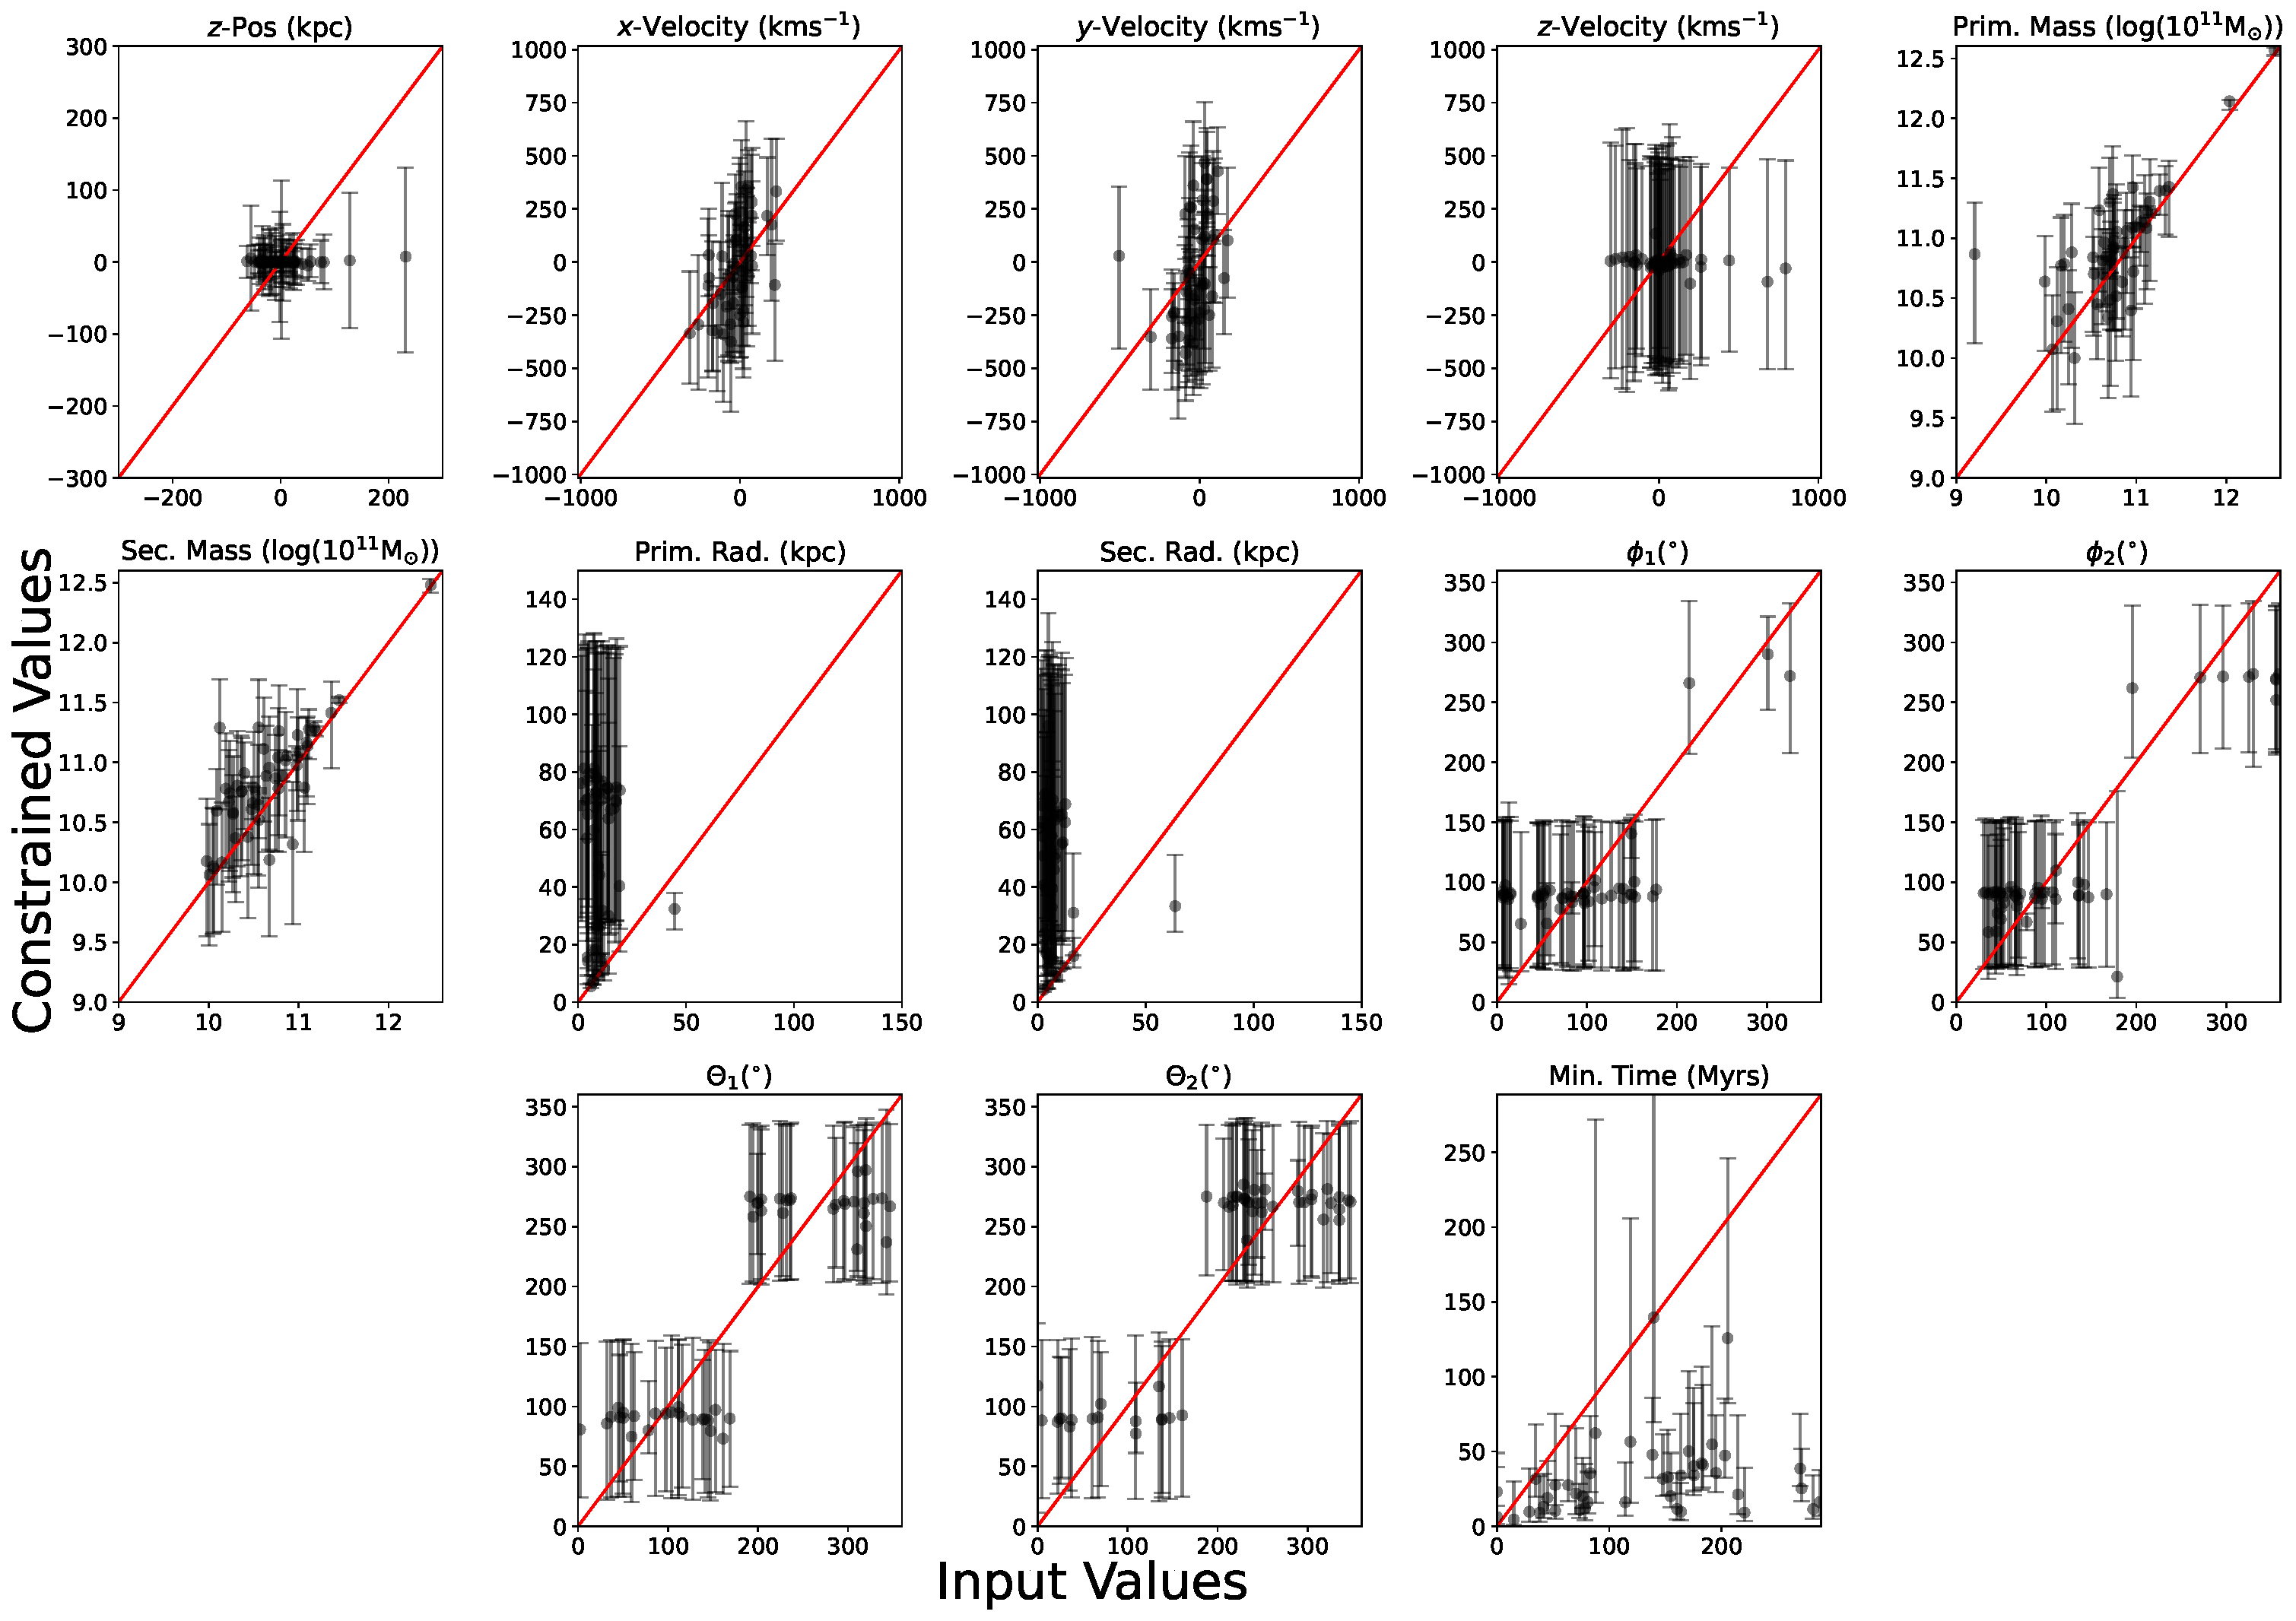
\includegraphics[width=\textwidth]{Chapter1/figures/51_51.pdf}
    \caption[The distribution of parameter values used to create our synthetic interaction images and the best-fit values we recover from our algorithm.]{The distribution of parameter values used to create our synthetic interaction images and the best-fit values we recover from our algorithm. The constrained values are taken as the 50th percentile of our walker distribution. Our lower and upper errors are then calculated as the difference from our best found value and the 16th and 84th percentiles, respectively. This gives an idea of the extent of our walker distribution in 1D. The red lines show a 1-1 relation and where our points would lie if the 50th percentile represented the exact input value found. Parameter names and unts are found in the title of each subplot.}
    \label{fig:true-found-parameters}
\end{figure*}

% Here, discuss Figure 13 in all its glory.
Figure \ref{fig:true-found-parameters} clearly shows where our MCMC has made excellent constraints and where it has not. The best constraints are on the masses of the interacting systems, where each best-fit value approximately follow the 1-to-1 relation. Where there is some discrepancy, the true values are within our errors. There is a trend here, however, that the total mass of the system is over estimated when compared to the true value. We also find excellent constraints on the majority of the positional and velocity vectors of the interaction, where the 50th percentile value approximates the true value. However, in these parameters we have explored a very wide parameter space when the majority of the true values are clustered around the centre of the parameter space. We will require further investigation with interacting systems more representative of the full parameter space we have explored. 

We also have reasonable constraints on our orientation parameters. As we often have two areas of high probability due to degeneracy, we opt to only plot the 50th percentile and errors of the high probability space near the input value. This would not be possible with an observational system with unknown parameters. Therefore, the user will either need to make a choice of what area of parameter space to explore, or input some prior on the orientation / inclination of the system. Once we have accounted for the degeneracy, we find that our 50th percentile value is representative of the true value, with the true value being within error of it. 

There are three parameters remaining where we find poor constraints or struggle to recover the true parameter value in general. The first are the radii of the two galaxies. We find that these are often over-estimated. Upon inspection of many of the output simulations, we find this is likely an effect of the distribution of particles and that we are using idealised synthetic images with no noise in the image. The way in which the particles are distributed is with an exponentially declining disk. This is achieved by creating a disk of particles which are sectioned into rings. Each ring has an exponentially declining probability of particles appearing within it based on the radius from the centre. Therefore, we find the outer rings of the galaxy are diffuse of particles, and do not dominate the likelihood function at high radius. This, in turn, means that galaxies with large angular size can be calculated as likely if the inner parts of the galaxy, with high particle numbers, match the flux of the inner disk. This also explains the over-estimate of the mass of each system. There are likely less particles than expected still within the galactic disk, and therefore more mass (ergo, luminosity) is required to keep the flux matched in the disk.

We also find we often under-estimate the time since the closest point of the encounter - i.e., the time of the passage - by a large margin. While those synthetic images whose underlying parameters had their point of passage very recently we recover very well, those at larger values we fail to. This is due to the likelihood function finding equivalent, high probability values between systems with correct tidal features and simple disks which match the inner disk of the interacting system. The former, tidal feature formation, requires a high $\beta$ parameter with low velocity and low impact distance. However, if the system is fast and does not form tidal features, but ends the simulation in the right place with the correct flux, the calculation will be dominated by the inner disk. Thus, we find a radius that covers the inner parts of the galactic disk successfully, with little disturbance that matches the flux of a large part of the galaxy. Therefore, the $\beta$ parameter is of the utmost importance to filter out these galaxies and give weight to higher t$_{\mathrm{min}}$ values.

Aside from the points that have already been raised regarding our MCMC constraining each parameter, a further problem was that the likelihood calculation is dominated by contributions from the mass and velocity parameters. Therefore, to continue improvements on other parameters further walkers and a longer chain must be run, incurring a cost of far more computation time. For the purposes of this work, we show the full degeneracy, limitations and difficulties of our model and what is to be expected in the most general case. Many of these limitations and problems can be resolved from tighter priors with more information regarding the systems being investigated.

The true power of this approach will be when investigating large populations of interacting galaxies and combining and marginalising over many different posteriors. When combining the parameter spaces of many different systems, it will be possible to identify those areas of parameter space which lead to the formation of certain features across populations of interacting galaxies. Our method will allow more intense simulations to sample smaller parameter spaces and be more efficient when finding systems with specific features. However, how to combine the posteriors is somewhat up for debate. We have ensured that the parameter spaces we are exploring are equivalent in size and that the prior is equal across parameter space. This introduces the question of the $\beta$ parameter in filtering simulations which, indirectly, changes the prior based on the trajectory of the interacting system. To conduct this combination, we would recommend that the $\beta$ parameter was not utilised when building the different posteriors if the increased computational cost is viable.

However, all of our results so far have been in the best-case scenario of a noiseless best fit simulation. The translation from simulation to observation in previous algorithms such as these is never an easy one. We, therefore, use our top three best fit systems here (Arp 172, Arp 240 and Arp 290) and apply our pipeline to their reduced observations.

\subsection{Applying to Observations}
% Brief re-iteration of creating observations.
\noindent We apply our MCMC to the reduced observational data of Arp 172, Arp 240, Arp 256, Arp 290 and Heart. Cutouts were created as described in Section \ref{data:obs-prep}. We reiterate here that the cutout resolution is reduced from its native resolution to cutouts of 100 $\times$ 100 pixels. Before we input the images into the pipeline, we find the central pixel of the secondary galaxy and convert this into a physical $x$- and $y$-position. We also find the total size physical size of the cutout in kpc, convert it to simulation units and provide this to the pipeline. We find that the physical size of the cutouts are significantly different from those of our synthetic dataset. As an example, we create the cutout of Arp 240 at 600 $\times$ 600 pixels at native resolution. With SDSS data, this corresponds to a physical size of 111.50kpc $\times$ 111.50kpc at the redshift of Arp 240. The synthetic image we previously used of Arp 240 is 785.35kpc $\times$ 785.35kpc. Figure \ref{fig:arp240} clearly shows a very different scaling between the observation and simulation, however, it is not enough to be seven times zoomed in on the system. We also find that the secondary positions are very different between the observation image and that used previously. As a result, the parameters we will find for constraining the observation will likely be very different. 

% Why do we take significantly longer on these?
We apply our MCMC to those outputs which had varying constraint. We only investigate these five systems as we find the computational expense is significantly higher when constraining the observations compared to the best fit simulations. We find the reasons for these are two fold. First, we must run each walker for twice the number of steps than when constraining the synthetic images to reach convergence. This is from increased noise contributions in the observation images. Second, due to the smaller scale size of our images, the defined $\gamma$ parameter is much stronger than with the synthetic images. Both of these reasons for higher computational expense are to be expected. The increase in the $\gamma$ parameter leads to us filtering out less candidate systems and running the base simulation code more often. This directly translates into a higher runtime for our MCMC.

% What do we find immediately?
Figure \ref{fig:obs_corner_plot} shows the reduced corner plot for the observed Arp 240 system. The constraints on the velocity parameter have significantly worsened when compared to the constrains on the best fit simulation. They are also in a different area of parameter space when compared. The velocity and spatial parameters are the most likely to be affected by the change in scale between the two input images. As the secondary galaxy position has been completely altered the best fit trajectory of the interaction has also completely changed. The secondary is significantly closer to the primary, therefore meaning the secondary velocity must be significantly slower than previously. Due to the increase in noise in the observational image, and the extent of the tidal features of the primary and secondary galaxies, the constraint has also significantly weakened.

\begin{figure*}
    \centering
    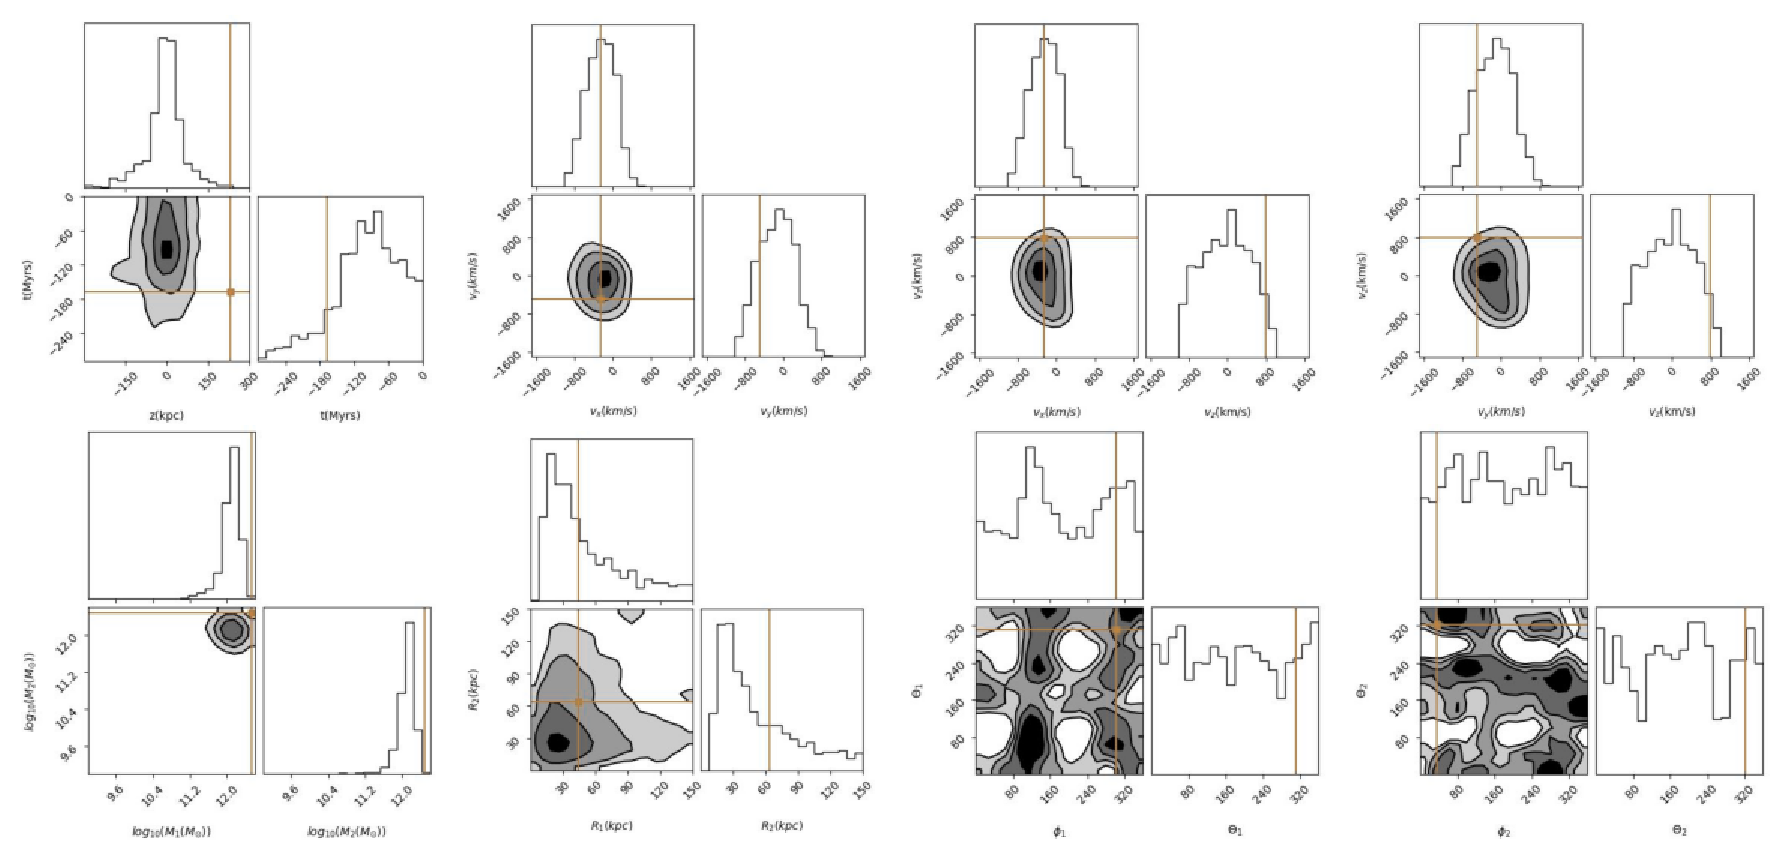
\includegraphics[width=\textwidth]{Chapter1/figures/Arp240_obs-red-corner.pdf}
    \caption[Reduced corner plot of the constraints made on the observational image of Arp 240.]{Reduced corner plot of the constraints made on the observational image of Arp 240. As shown, there is significant additional uncertainty in these measurements than those of the best fit simulation. However, we are able to make constraints on almost all parameters in the sample. The degeneracy in the orientations remains. The gold lines represent the true values we used in to create the synthetic image.}
    \label{fig:obs_corner_plot}
\end{figure*}

However, for the remainder of the parameters the level of constraint remains similar even with the change in the best fit values. We retain the two- and four-fold degeneracy in the orientation parameters. This follows on that the pipeline outright rejects disks which are edge on and loses accuracy when attempting to pin point the precise inclination of each galaxy. We are unable to make any constraint on the $\theta$ parameters, while the degeneracy of the $\phi$ parameters is still visible. The radius parameter is well constrained at 11.8\% CI, although with large tails in the probability space for both the primary and secondary galaxies. These tails are significantly larger here than when using the best fit simulation as the input. This is due to the observation image having no hard cutoff of the edge of the galaxy, and simply moving into more noise. The outer edges of our simulated galaxies also moves to very low signal, and therefore, there is lots of uncertainty surrounding the true radius of the galaxy. 

We, again, make excellent constraints on the mass parameters. The accuracy in the flux distribution of the primary and secondary disk is what dominates here, and therefore, we find this value incredibly quickly. The found value is comparable to the best fit simulation, although slightly lower. We also compare our constrained values to what is found in the literature. Using the criteria described previously, we recover total masses of $\frac{M_{1}}{10^{11}M_{\odot}} = 7.97 - 15.9$ and $\frac{M_{2}}{10^{11}M_{\odot}} = 8.1 - 16.2$ which correspond to stellar masses between $\frac{M_{1,*}}{10^{11}M_{\odot}} =  0.94 - 1.89$ and $\frac{M_{2, *}}{10^{11}M_{\odot}} = 1.0 - 1.9$ in our simulations. These are slightly higher than literature values, with a recent work quoting the stellar mass as $\frac{M_{1, *}}{10^{11}M_{\odot}} = 0.94 $ and $\frac{M_{2, *}}{10^{11}M_{\odot}} = 1.05$ \citep{2020MNRAS.496.5243H}. Thus, while our 50th percentile value is higher than the measured values, we do recover them within error.

This is true in the Arp 172 and Arp 290 observational constraints as well. The synthetic image we have used is at a different scale when compared to the the SDSS observations. We therefore end up with similar constraints to the different parameters, however with significant variation in the spatial parameters. The uncertainties in the radius parameters are significantly increased, while the constraint on the $\theta$ parameters is completely lost. In fact, for the same number of steps compared to constraining the best fit parameters, our MCMC fails the Geweke diagnostic. Therefore, due to the added noise running longer chains is imperative which drives up computational expense.

This leads us onto the limitations of this process to constraining galaxy interaction. While it has been very successful for many of the underlying parameters, there are many different parameters which must be provided to the pipeline so it is able to make those constraints. We discuss the limitations of applying this methodology to large interacting galaxy datasets, and how these can be offset in the short term but a long term solution is still required.

\subsection{Limitations}\label{limitations}
\noindent While this methodology does show a lot of promising in being able to constrain underlying parameters across populations of interacting galaxies, it is important to note that at its base is a restricted numerical interaction code with limited resolution. There may be some interacting systems that simply cannot be modelled realistically using three-body approximations, and may therefore cause a skew in results. However, there are also some more subtle limitations which may affect how a user wishes to use this MCMC approach.

\subsubsection{Resolution \& Depth Effects}\label{resolution_effect}
\noindent One of the fundamental parameters that must be provided for this methodology to work is the redshift of the system. This is used to calculate the distance to the system and then converted to an assumed resolution for the scale of the image. If this is input incorrectly the simulation images will be created at an incorrect resolution, and the MCMC will likely not reach convergence. This is also true of providing and calculating correctly an approximation of the position of the secondary galaxy. Significant computation power can be wasted if these parameters are incorrect, and will give spurious results. The reduction in resolution of the images is also an important limitation. This toy model needs small, thumbnail size images with a reasonable number of degrees of freedom as to reach convergence. Therefore, input images can only be of limited resolution which will affect the quality of the constraints we can actually make on different systems. 

The redshift is also used in scaling the fluxes calculated for each particle in the simulation. The base SED is calculated for a 1 M$_\odot$ system at a distance of 10pc. This is then scaled to the mass assigned to a particle and then put at the distance calculated from the redshift. If the redshift is incorrect (or even slightly off) then this could lead to a bad fit for the mass of the two galaxies in the system. A flag exists in the algorithm to give it the freedom to slightly vary the redshift (and therefore the distance and resolution) by 0.001 with each step. It will then attempt to fit the redshift and resolution of the system. Note, however, this is untested and currently significantly increases computational expense.

Depth effects also play a significant role in the ability of our algorithm to fit a system. For this work, we used primarily synthetic images, meaning we were not at risk of this. However, when using observational imaging this could become a significant problem. Our observational examples were of major interacting systems which resided in the high surface brightness regime, where we retained the full extent of the tidal features and could provide better fitting. However, for systems that lie closer to the low surface brightness regime, our algorithm will become less efficient and require more computational expense to make effective constraints.

This also has the opposite effect in terms of tidal features formed. For example, if a system is being fit but at the true parameters a tidal feature exists which has not been detected due to its low surface brightness then our MCMC pipeline will not be able to converge on the true values. The algorithm would instead converge on those parameters where the disks were at the correct flux rather than getting the tidal features correct. Therefore, when exploring the parameter space of interacting systems with our pipeline, it is imperative that the full structure is within detection of the observing instrument.

There must be a trade off between the resolution of our simulation and the observations. In this work, we used cutouts of 100 $\times$ 100 pixels. This was so that we could still get consistent system outputs from our simulations using only 2500 particles. If lots of pixels are used, then using a low number of particles can lead to many `unphysical' output simulations. I.e. these are simulation systems where the disks will have large holes in them where there haven't been enough particles to fill the disk. To mitigate the effect of potentially using low particle numbers, we distribute the flux as described in Section \ref{flux_dist}, which is an imperfect solution. It is recommended for any user to make a balanced trade off between resolution and computational expense.

\subsubsection{Computational Expense}\label{computational_expense}
\noindent The main drawback of this methodology is that of computational expense required to run such an MCMC over a the full parameter space. In the case of this work, the simulation was set up with 2500 particles on a High End Computer Cluster with 50 CPUS. Each simulation took approximately two seconds, with the full sample run taking approximately 30 days to complete. Each galaxy was given 600 walkers to move through parameter space with each walker moving 7,500 steps. The highest memory requirement of any system was 6GB. Therefore, the runtime is very high but the memory required for it is approximately 122MB per core.

This methodology was successful in constraining 51 different interacting galaxy synthetic images. Achieving the same in prior work projects, such as Galaxy Zoo: Mergers, took months to complete. We have reduced the runtime required of it to 30 days on a powerful High End Computer Cluster. However, this is not the solution to the large scale dataset problems that we will be seeing when LSST comes online. If we are to run this methodology on a much larger galaxy sample - such as thousands of galaxies - then we will need to find ways to significantly improve the runtime of this method.

\section{CONCLUSIONS \& FUTURE WORK}\label{Conclusions}
\noindent In this work, we have introduced a new algorithm based on a MCMC framework to apply constraints on the underlying parameters of interacting galaxies. We have made these constraints, and explored the underlying parameter space, through directly comparing input images to output simulations. Thus, we have mapped the underlying parameters that define interaction to an output morphology that we compare for similarity with a synthetic or observation image of an interaction. We have introduced an updated version of the restricted three body simulation JSPAM and modified it to calculate and match the flux distribution of interacting galaxies based on thirteen underlying parameters. This updated algorithm, APySPAM, calculates the flux distribution by assigning particles with a spectral energy distribution and accounting for star formation throughout the interaction. 

% Look at the tense mash up of the below paragraph.
To test our MCMC, we applied it to a set of synthetic images of interacting systems created from the parameters found in the Galaxy Zoo: Merger project for a set of real interacting systems. We were able to recover the true parameters used to create these images, with associated error measurements on each. We have explored the specific results of a single synthetic image: that of the Arp 240 system, and shown the corner plots and full posteriors of each parameter. We have took the 50th percentile value as the best fit value for our synthetic dataset, and used the 16th and 84th percentile to define the errors on our measurements. We then presented the distribution of our recovered underlying parameters and the true values, describing the general trends in our methodology as well as its limitations. 

Every parameter of our thirteen was recoverable, however there was significant degeneracy in the orientation angles of the two galactic disks. This was expected as works such as \citet{2010ASPC..423..227S} found significant degeneracy between systems, but not a direct cause. In this work we found, without taking account of kinematic information, multiple orientation angles can recreate observed tidal features as well as limitations in the pixel matching method of constraint. When tested on observational data of our best fit synthetic systems, we were able to retain the excellent constraints on nine of the thirteen parameters, but lost any constraint on the orientations. However, we were able to maintain a tight constraint on the masses of the two systems. 

There are limitations to this method that any users must be aware of. First, the core simulation of this process is a restricted three-body code with a highly optimised flux distribution calculation and approximation. It is probable that there are systems that this approach can not constrain, or may give nonphysical results for. The required reduction in the parameter space of the images, such as reducing the degrees of freedom and limiting individual pixel resolution in favour of computation time, also may lead to constraints only on the disks of the galaxies and not the tidal features themselves. There is also limited time and spatial resolution within the simulation itself. When using true observations, they had to be artificially scaled up so our simulation could maintain the resolution to have constraint. In terms of the temporal and spatial parameters, this scale up can be accounted for. However, in terms of the masses of the flux distribution, this can be significantly hindered. Therefore, a user must be careful when choosing the image scales to use when attempting to constrain individual systems. 

We have demonstrated the power of this methodology, and that it is capable of recovering the underlying parameters of interaction in idealised examples. The next, serious test of this MCMC approach will be to use it on a set of observed interacting systems, where the underlying parameters are known to properly diagnose the results. However, completely constrained interacting galaxy samples are only of a small scale and few exist. We will apply our MCMC to the observed dataset of our 51 interacting systems in SDSS.

This is an initial step towards developing the methodology to serve the field as large scale surveys - such as LSST - come online. Large scale automation where we can constrain interaction, make diagnostics and estimates about parameter space are not only important for inferences about individual datasets but for the interacting galaxy population as a whole. The main limitation of this method is the computational expense associated with it. To run this on 51 systems, the total run time was thirty days; an unusable timescale when being applied to interacting galaxy samples in the thousands. Therefore, future works with this algorithm and methodology will also be focused on increased computational efficiency and working on larger interacting galaxy datasets. 

The bottleneck for computational efficiency lies in the time spent running the APySPAM simulation. While incredibly cheap individually, this is exceptionally expensive when having to be run in an MCMC chain. With the growing power of GPUs, and their ability to run numerical simulations significantly more efficiently than CPUs, a pathway to solve this limitation may already exist. This, combined with further developments in methodologies such as simulation based inference, machine learning and gaussian processes could begin to reduce computation time.
\chapter{Advanced PySPAM: An Infrastructure to Constrain Underlying Interacting Galaxy Parameters}\label{chapter4}
\section{Introduction}\label{Introduction}
% Introduce interaction, and why it's important.
\noindent The precise interplay between the observed processes we have discussed in this thesis and the underlying physical parameters of the involved galaxies is difficult to quantify. Using large scale observational datasets allows us to probe this relation, but without the ability to constrain the dynamical timescale the precision of our constraints on it remains limited. Algorithms have been developed to match the underlying parameters of an interaction and its dynamical timescale by directly modelling the expected final morphology. If a simulation of an interaction can reproduce the final morphology, then it has likely correctly inferred the interaction over the dynamical time.

Examples of algorithms designed to make this matching include Identikit by \citet{2009AJ....137.3071B} or the Stellar Particle Animation Module (SPAM) by \citet{1990AJ....100.1477W}. However, finding the best fit underlying parameters for more than a handful of systems is often seen as unfeasible. There are often greater than 10 different parameters which contribute to different observed morphologies. This leads the underlying parameter space to be greater than 10-dimensional and complex. Exploring even a sub-space of this parameter space fully requires tens of thousands of models to be run. This is also hindered by its degeneracy. For example, \citet{2010ASPC..423..227S} found that four of their best-fit models were able to accurately match morphology of the Arp 284 system. Therefore, it is often preferable to use large cosmological simulations \citep[e.g.][]{2015MNRAS.446..521S, 2018MNRAS.480..800H, 2020MNRAS.493.3716H} to create large samples of synthetic interacting galaxies where analogues to the observed system can be found. This, however, limits our capability to explore observational parameter space beyond the limitations of such cosmological simulations. By their nature, cosmological box simulations have finite scope and size; meaning the rarest (and likely most fundamental) interacting systems will remain unexplored without significant further computational expense.

This limitation of directly comparing numerical simulations to observations was solved in a novel way by \citet{2016MNRAS.459..720H} in the Galaxy Zoo: Mergers (GZM) project (for details on Galaxy Zoo, see \citet{2008MNRAS.389.1179L}). GZM worked with citizen scientists to run simulations of interaction and visually compare the simulated morphology to observations. GZM studied a sample of 62 interacting galaxies from the Arp catalogue of interacting galaxies \citep{1966ApJS...14....1A}. Citizen scientists' were given a selection of simulation outputs around an observation and would select the one which appeared most alike. The simulations would then be run again with tweaked underlying parameters with the citizen scientist selecting the new the best fit output. With enough citizen scientists on the project, enough new simulations run and enough time GZM were able to find the best fit parameters for their interacting galaxy sample across a 14-dimension parameter space. This created the largest fully constrained interacting galaxy samples to date. In the era of the Vera C. Rubin Observatory such an approach will not be practical, with statistically significant samples of thousands of interacting galaxies potentially being produced every week, a new approach is required.

In this Chapter, we present an automated methodology to constrain the underlying parameters of interaction. We combine a fast restricted numerical simulation code with a Markov-Chain Monte Carlo (MCMC) framework. We apply this over a 13D parameter space and constrain the probability distribution and find the likely parameter values describing an interacting galaxy system. This approach allows us to marginalise over each parameter, provide the best fit value as well as the error on each measurement. First, we apply this to a set of synthetic interacting galaxy observations created from a restricted N-body simulation where we have input the 13 underlying parameters. This provides us with diagnostics of our methodology. We then apply our process to five real observations of interacting galaxies and discuss how our methodology could be applied to real data, and the limitations therein. We also discuss the more general limitations of this approach, with a particular emphasis on the computational expense required, and the potential future solutions.

% Layout of document/
The layout of this Chapter is as follows. In Section \ref{Data}, we describe the sample of 51 galaxies we will study and our approach to observation preparation. Section \ref{Methods: sims} will summarise our simulation code and how it has been updated from previous iterations. We also describe how we build our sample of synthetic interacting galaxies and the parameter space we will explore with this simulation. A full discussion of our results will be given in Section \ref{Results} followed by our conclusions and future work in Section \ref{Conclusions}.

\vspace{-5mm}
\section{Data}\label{Data}
% What is the data?
\subsection{Sample of Major Interacting Galaxies}
\noindent In this work, we test our Markov-Chain Monte Carlo (MCMC) process on idealised, mock observations of 51 major interacting systems. These mock observations are created using our numerical simulation where we have input the underlying parameter values directly. As we know what the true underlying parameters of each interaction are, we can test the accuracy of our MCMC. To create these mock observations, we use the underlying parameters found in the GZM project for 62 interacting galaxies.

Of the 62 systems, we create synthetic images of 51 of them to act as our idealised observational sample. As we are including the flux distribution of each system, we require an accurate redshift of each system. 3 of the 62 systems do not have a redshift measurement in the NASA Extragalactic Database (NED), the Sloan Digital Sky Survey (SDSS) or Simbad databases. Therefore, we discard these. We create each mock observation as though it was observed using SDSS. Of which, a further eight systems are not present. Therefore, we also discard these systems. This leaves us with the GZM best-fit parameters of 51 systems with which to create our synthetic observations. The details of the real systems are displayed in Table \ref{tab:Objects}, including the target coordinates, the SDSS ID and the redshift measurements we use. How we create our synthetic images is described in Section \ref{sec:syn_sample} after we have described our simulation.

\begin{table*}
    \centering
    \resizebox{0.79\textwidth}{!}{\begin{tabular}{|c|c|c|c|c|c|c|}
    \hline
         Name & SDSS ID & RA & Dec & Redshift \\
         \hline
         Arp 240 & 587722984435351614 & 204.980417 & 0.835278 & 0.02250 \\
         Arp 290 & 587724234257137777 & 30.946317 & 14.72365 & 0.01171 \\
         Arp 142 & 587726033843585146 & 144.429583 & 2.763056 & 0.02329 \\
         Arp 318 & 587727177926508595 & 32.380516 & -10.158508 & 0.0132 \\
         Arp 256 & 587727178988388373 & 4.710417 & -10.369167 & 0.02730 \\
         UGC 11751 & 587727222471131318 & 322.247796 & 11.382539 & 0.02909 \\
         Arp 104 & 587728676861051075 & 203.037083 & 62.733889 & 0.01082 \\
         Double Ring, Heart & 587729227151704160 & 238.287292 & 54.147861 & 0.040 \\
         Arp 285 & 587731913110650988 & 141.040000 & 49.226111 & 0.00967 \\
         Arp 214 & 587732136993882121 & 173.145221 & 53.067922 & 0.00331 \\
         NGC 4320 & 587732772130652231 & 185.740516 & 10.548328 & 0.02668 \\
         UGC 7905 & 587733080814583863 & 190.952917 & 54.900278 & 0.01648 \\
         Arp 255 & 587734862680752822 & 148.290000 & 7.870000 & 0.04106 \\
         Arp 82 & 587735043609329845 & 122.811250 & 25.193056 & 0.01368 \\
         Arp 239 & 587735665840881790 & 205.423852 & 55.672324 & 0.02489 \\
         Arp 199 & 587736941981466667 & 214.265833 & 36.573333 & 0.01024 \\
         Arp 57 & 587738569246376675 & 199.198750 & 14.424444 & 0.048 \\
         (HWB2016)Pair 18 & 587738569249390718 & 206.209583 & 13.921361 & 0.089 \\
         Arp 247 & 587739153356095531 & 125.889478 & 21.342976 & 0.01108 \\
         Arp 241 & 587739407868690486 & 219.461958 & 30.481222 & 0.03472 \\
         Arp 313 & 587739505541578866 & 179.418333 & 32.285556 & 0.01045 \\
         Arp 107 & 587739646743412797 & 163.069583 & 30.065278 & 0.03318 \\
         Arp 294 & 587739647284805725 & 174.931624 & 31.920108 & 0.00892 \\
         Arp 172 & 587739707420967061 & 241.389583 & 17.597222 & 0.029 \\
         Arp 302 & 587739721376202860 & 224.251667 & 24.612222 & 0.03286 \\
         Arp 242 & 587739721900163101 & 191.544583 & 30.727222 & 0.02205 \\
         Arp 72 & 587739810496708646 & 236.733750 & 17.878333 & 0.01100 \\
         Arp 101 & 587739845393580192 & 241.124946 & 14.800192 & 0.026 \\
         Arp 58 & 587741391565422775 & 127.990209 & 19.211523 & 0.03722 \\
         Arp 105 & 587741532784361481 & 167.804167 & 28.724722 & 0.021 \\
         Arp 97 & 587741534400217110 & 181.439583 & 31.068889 & 0.02305 \\
         Arp 305 & 587741602030026825 & 179.655833 & 27.490833 & 0.004 \\
         Arp 106 & 587741722819493915 & 183.902522 & 28.173576 & 0.02199 \\
         NGC 2802/3 & 587741817851674654 & 139.172619 & 18.963463 & 0.02914 \\
         Arp 301 & 587741829658181698 & 167.470000 & 24.259722 & 0.02059 \\
         Arp 89 & 587742010583941189 & 130.665852 & 14.285624 & 0.00687 \\
         Arp 87 & 587742014353702970 & 175.185000 & 22.437778 & 0.02373 \\
         Arp 191 & 587742571610243080 & 166.834167 & 18.431111 & 0.02739 \\
         Arp 237 & 587745402001817662 & 141.933458 & 12.286750 & 0.02899 \\
         Arp 238 & 588011124116422756 & 198.886667 & 62.126944 & 0.03106 \\
         MCG +09-20-082 & 588013383816904792 & 181.161667 & 52.956111 & 0.078 \\
         Arp 297 & 588017604696408086 & 221.330417 & 38.761389 & 0.0298 \\
         NGC 5753/5 & 588017604696408195 & 221.328663 & 38.805889 & 0.01374 \\
         Arp 173 & 588017702948962343 & 222.869434 & 9.328297 & 0.028 \\
         Arp 84 & 588017978901528612 & 209.649167 & 37.438889 & 0.01158 \\
         UGC 10650 & 588018055130710322 & 255.060770 & 23.106346 & 0.00986 \\
         Arp 112 & 758874299603222717 & 0.368333 & 31.437778 & 0.024 \\
         Arp 274 & 587736523764334706 & 218.786250 & 5.356389 & 0.02890 \\
         Arp 146 & 587747120521216156 & 1.685000 & -6.635833 & 0.07544 \\
         Arp 143 & 588007005230530750 & 116.72333 & 39.019444 & 0.01374 \\
         Arp 70 & 758877153600208945 & 20.864583 & 30.778333 & 0.03500 \\
         Arp 218 & 587739720308818095 & 238.397500 & 18.607222 & 0.075 \\
         \hline
    \end{tabular}}
    \caption[The names, SDSS ID, right ascension, declination (in degrees) and redshift for the 51 interacting systems we will examine.]{The names, SDSS ID, right ascension, declination (in degrees) and redshift for the 51 interacting systems we will examine. All redshifts are as found on the NASA Extragalactic Database.}
    \label{tab:Objects}
\end{table*}

\subsection{Observation Preparation}\label{data:obs-prep}
\noindent To robustly test our MCMC algorithm, we will constrain the underlying parameters of observations of a subset of the systems described in Table \ref{tab:Objects}. Therefore, we describe how we build such observational images here. We downloaded the FITS files from SDSS Data Release 16 which contained the full system of interacting galaxies. These were then used to create smaller cutouts of the systems. The coordinates of the primary galaxy are used as the center of the image. We judged the size of the cutout by the size of the full interacting system, most often between 600 - 1000 pixels. We created cutouts in each SDSS filter ($ugriz$).

We convert each observational image into counts from the native unit of nanomaggies using the conversion value in each FITS header. Each filter image was then stacked into white image by simply summing them together. This gave us a higher signal-to-noise in the tidal features of the interacting systems. Then, we took these native resolution white images and block reduced them to a 100 $\times$ 100 thumbnail. Each cutout was visually inspected to ensure that, even with the reduced resolution, the tidal features were still clear and prominent in the image.

We take the 0.396" pixel scale of SDSS on the sky with the measured redshift to calculate its physical size. From the pixel-to-distance conversion for each image, the position of each secondary galaxy was calculated from the central pixel. No attempt was made to approximate the $z$-position of the secondary galaxy, as this is a parameter to constrain. In total, there are 13 parameters that we must constrain over our synthetic and observation images. These parameters are detailed in the following section. The observation image preparations were made using the Astropy Python package \citep{astropy_2013, astropy_2018}.

% Describe what GZ: Mergers found and what we're going to do that is different.
% This should perhaps be in the Introduction if it isn't already.
\section{Simulating Galaxy Interaction}\label{Methods: sims}
\noindent We require a method of mapping underlying parameters to our observed systems morphology and calculating how likely it is they are representative. We input our set of underlying interaction parameters into a restricted three-body simulation which predicts the morphology and flux distribution of the interacting system. In this section, we describe our simulation code, its previous iterations and how we add in additional flux information.

\subsection{APySPAM}\label{sec:simulations}
% What is it?
\subsubsection{Restricted Three-Body Simulation}\label{sec:apyspam}
The simulation code we use is the Java Stellar Particle Animation Module (JSPAM) \citep{2016A&C....16...26W}. For an in-depth description of the underling code, we direct the reader to \citet{1990AJ....100.1477W,2016A&C....16...26W} but provide a summary here. JSPAM is a restricted three-body code focused on recreating the morphology of interacting systems. It approximates the interaction as two massive bodies each being orbited by a set of massless test particles. The gravitational potential of the two massive bodies and the resultant forces upon the massless test particles is calculated and used to predict the particles position and velocity at different timesteps. The size and number of time steps can be input by the user. JSPAM is computationally efficient, approximating the morphology of an interacting system using thousands of particles in seconds on a regular work PC at a reasonable time resolution. The primary particle integrator is a fourth-order Runge-Kutta which applies backwards integration to calculate the position and velocity of the massive bodies from t=0 to the time set by the user. The test particles are then added to the simulation, and forward integration is conducted to find their position and velocity in each timestep through the trajectory of the massive bodies. In this way, a flyby of the two galaxies is simulated with the test particles representing the extended morphology of the two galaxies. 

The user has the option to choose a N-body approximation or a softened point mass approximation. Each of these slightly changes the way that the integrator calculates the forces on each particle. Therefore, there will be slight discrepancies between the final morphology of systems interacting with the same underlying parameters but different force approximations. We elect to utilise the softened point mass approximation, as this has improved computational efficiency over the higher accuracy of N-body approximation \citep[for more on this see][]{2016A&C....16...26W}. 

The base code of JSPAM was purely a morphology matching code. Attempting to extract underlying parameters of interaction from morphology matching alone has been shown in prior works to be difficult \citep[e.g.][]{2009AJ....137.3071B}. JSPAM itself has been used in genetic algorithms to find the best fit parameters of different systems \citep[e.g][]{2023A&C....4200691W}. However, this lacks the exploration of parameter space and the quantification of uncertainties we aim to achieve in our approach. Using both morphology and flux matching between simulations and observations improves accuracy of recovered parameters \citep{2021ApJ...923..124M} and we have therefore enhanced the original JSPAM algorithm with the ability to model population evolution with star formation/star bursts to approximate the flux distribution of the interacting system. We have created this enhanced version in Python 3.7.4 (hence, we shall refer to this algorithm as Advanced Python Stellar Particle Animation Module, APySPAM).

To approximate the flux distribution of the galaxies in the simulation we calculate luminosity of each particle while minimising the computational cost. We incorporate the evolution of the underlying stellar populations of each galaxy over the time taken in the interaction. We also incorporate the formation of new stellar populations in potential starbursts, and approximate the impact this will have on the galaxy flux distribution. To preserve the computational efficiency, we build a semi-analytic model and define a global stellar population to assign a luminosity to each particle based on its assigned, hypothetical mass. In this way, we `paint on the stars' of each galaxy without having to directly model stellar evolution and star formation. This process is detailed in the following two subsections. 

% Why is it different from the original JSPAM?
% Overview of APySPAM:
\subsubsection{Stellar Population Evolution}\label{Stellar_Pop_Evol}
To model the underlying stellar populations, we utilise a \citet{2003MNRAS.344.1000B} (BC03) simple stellar population. These contain SEDs generated from flux libraries from a \citet{2003PASP..115..763C} initial mass function. We set this stellar population model to have a delayed exponentially declining star formation rate \citep{2009ApJ...690..802J, 2013ApJ...762L..15P,2014arXiv1404.0402S, 2019A&A...622A.103B}. However, to capture any star formation due star formation enhancement in the interaction, we increase the star formation based on the conditions in the interaction. We assume an e-folding time for star formation of $\tau = 1.7\text{Gyrs}$. This value is chosen as it matches field, massive galaxies found in the literature \citep[e.g][]{2010ApJ...721..193P} and used in hydrodynamical simulations \citep[e.g.][]{2022ApJ...941....5J}. Our simulation outputs a spectrum normalised to 1M$_{\odot}$ with each particle initially assumed to be the same age as the galaxy.

This spectrum must then be scaled to the stellar mass present at each particle. We follow the prescription as stated in \citet{2016A&C....16...26W} to distribute the mass between the three components of the galaxy, and then to each test particle. The galaxy in the JSPAM simulation has its mass distribution as $M_{\text{bulge}} = 0.05M_{\text{galaxy}}$, $M_{\text{disk}} = 0.14M_{\text{galaxy}}$ and $M_{\text{halo}} = 0.81M_{\text{galaxy}}$. We take the total mass assigned to the galaxy (input by the user) and divide it into these three components. We then assume that the bulge and disk masses are fully baryonic, with the remaining mass being non-baryonic dark matter. We further divide the calculated baryonic mass into two components: stellar and gas. The total stellar mass of each particle is used to scale our final output SEDs from our model while total gas mass of each particle is used to calculate the star formation rate. The gas and stellar mass to be distributed to the particles is then defined by a gas fraction parameter that the user can alter. By default, this value is 0.15 for both the primary and secondary galaxies.

We assume the initial ages of the galaxies (both 10Gyrs by default) at initialisation and calculate the final age of the SEDs based on the number of time units the user wishes to run the simulation. This age is then used to extract the normalised spectra from the BC03 templates. These output SEDs are then convolved with given telescope filters of the users choice and integrated, giving a colour flux value to each particle. However, this process only outputs the final flux values at each particle of the initial stellar population. During the interaction, we assume that the galaxy begins to form new stars at a rate significantly higher than is modelled in the BC03 templates. Therefore, we account for this by modelling newly created stellar populations as the interaction progresses.

To incorporate the increase in star formation in our simulations, we manually enhance the expected star formation rate through the simulated interaction. In high-resolution simulations which also model the evolution of gas, starbursts occur naturally \citep{2009PASJ...61..481S}. However, in our simulations we must approximate this behaviour in a semi-analytic fashion. The change in star formation is heavily dependent on the mass ratio and the kinematics of the interaction and, therefore, we implement an enhancement parameter based on these parameters. We calculate the excess star formation due to the interaction compared to what is already expected in the SED, and distribute this to each particle based on the initial gas mass. Approaching the problem in this semi-analytic way is similar to what is done in the CIGALE \citep{2019A&A...622A.103B} algorithm. Here, we detail this enhancement parameter.

At any given timestep the total stellar mass is given by
\begin{equation}\label{Total_SFR}
    SFR_{\text{enhancement}} = \beta (\frac{t}{\tau^{2}}) \exp(-\frac{t}{\tau}) M_{\text{baryonic}} M_{\odot} \text{yr}^{-1}.
\end{equation}
Here, $\tau$ is the e-folding time of star formation, $M_{\text{baryonic}}$ is the baryonic mass of the galaxy and t is the age of the galaxy at the given timestep. This is the star formation at any time given by the BC03 template. However, we include the $\beta$ parameter: our enhancement value. This is a dimensionless value given by
\begin{equation}\label{enhancement_param}
    \beta = M_{\text{ratio}} D_{\text{ratio}}^{2}.
\end{equation}
$M_{\text{ratio}}$ is the mass ratio between the galaxy being enhanced and the galaxy causing the interaction. D$_{\text{ratio}}$ is the ratio of each galactic radius to the distance between the galactic cores. In a system with a high mass galaxy interacting with a low mass galaxy, the high mass galaxy will have relatively little star formation enhancement while the less massive galaxy will have significant enhancement. This is similarly true for the ratio of the radius and separation. If the galaxies are interacting in such a way that the distance of closest approach is less than each galactic radius, then this ratio will rapidly increase above one; enhancing star formation further. This represents a significantly more violent interaction. It is important to note, however, that this has significantly less impact on strengthening star formation than that of the mass ratios. 

These parameters successfully reflect the findings of the current astrophysical literature, where mass ratio has a significantly higher role on star formation enhancement than impact parameter \citep{2003ApJ...582..668B, 2008MNRAS.391.1137L, 2008MNRAS.385.1903L}. We base our semi-analytic approach on the star formation histories found in a range of high resolution N-body simulations \citep{1996ApJ...464..641M, 2000MNRAS.312..859S, 2019MNRAS.490.2139R} which measure the change in star formation directly from the Kennicutt-Schmidt \citep{1998ApJ...498..541K} relation. These simulations directly model the star forming gas through the interaction, measuring the change its evolution which we are able to approximate. Thus, we achieve an accuracy comparable to directly-modelled simulations at a fraction of the computational cost.

The output of Equation \ref{Total_SFR} is global star formation of each interacting galaxies at any given timestep. However, the aim of our model is to be able to match the flux distribution across the entire galaxy (particularily the tidal features) to any observation that the code is given. Therefore, we must distribute the star formation throughout the particles. To keep computational efficiency, we utilise weights which have been assigned to each particle. These weights are based on the ratio of the gas mass of the particle which has been assigned at initialisation to the total gas mass of the galaxy. So, to find the star formation rate of a single particle at any given timestep, the following equation is applied,
\begin{equation}
    SFR_{\text{Particle}} = \frac{M_{\text{gas,Particle}}}{M_{\text{gas,Galaxy}}}SFR_{\text{Galaxy}}.
\end{equation}
After every time step, the gas within each particle is reduced by the mass converted into stars. Once this drops below a user defined value, the particle is cut off from star formation and is considered quenched. Currently, each particle is assigned equivalent gas mass at initialisation of the simulation. Therefore, when a particle is quenched in this example, every particle in the galaxy will also be quenched. The user can define a gas distribution model, which will lead to particles being quenched at different times.

There are limitations to this approximation. We assume that each galaxy is a disk galaxy prior to the interaction when we assign gas masses to each particle. We assume that all of the gas mass assigned can be used in star formation, i.e. all the gas is cold molecular gas. We make no account of gas ionisation or the turbulence in the ISM that likely occurs during these interactions. We also assume that the disruption occurring to the test particles represents what would occur to the gas disk of galaxies within an interaction. However, we find that with these assumptions, the output star formation histories mimic those simulations which directly calculate these values. 

Upon finding the star formation rate at the position of each particle, we convert this into a stellar mass formed through the timestep taken. We then compare this formed mass to the expected mass formed in the initial underlying stellar population. If the new mass formed is so low that it would be captured by the underlying population, we do not add this mass. If excess stellar mass has been formed, we assign an SED to it and its age is recorded. Once the simulation is completed, each new stellar population age is used to extract the relevant BC03 SED and multiplied by the total mass of the new stellar population. We then stack all of the SEDs together. This gives us the total extra emission we expect from the stars formed during the starburst throughout the simulation. This is then added to the initial stellar population emission defined at the beginning of the simulation. This gives us the total SED of each particle throughout the simulation. Each particle SED is then convolved with user inputted telescope filter responses and integrated. This gives a total flux that would be measured from each particle as if observed. 

Thus, with the underlying JSPAM code approximating the positional distribution of particles to the observed system, with APySPAM we paint on the flux and find the flux distribution. This allows us to directly compare the pixel in a simulation image to an input observational image. However, in doing so, a limitation was found due to using a particle number that was significantly less than the number of pixels.

\subsubsection{Extending Flux Distribution}\label{flux_dist}
\noindent One remaining challenge in the simulations is that we are attempting to model full interacting systems with a number of particles significantly less than the number of pixels in each image. This is to maximise computational efficiency. The resulting effect is that large gaps can appear in the tidal features that form or within the disks themselves as the interaction progresses. To mitigate this effect, we calculate the flux at each particle position and then use the procedure described below to distribute it through each pixel of our image. This results in more realistic images of galaxies compared to binning the particle flux based on position.

First, we calculate the flux at each particle described in the previous sections. We take each particle SED, and convolve it with the filter(s) of the user's choice. These convolved SEDs are then integrated to give a value of the flux in counts at each particle. We then create a grid of pixels and calculate the physical distances between each of their centres. We then calculate the contribution of flux from each particle to each pixel centre. Once the 2D flux distribution has been found across the pixel grid, we then use the measured redshift of the galaxies to find the measured fluxes as if the system had been observed.

The result of this is a well distributed galaxy image where there are no empty spaces in the tidal features nor in the disk. However, it does have a limitation when particles are not within the galaxy. When a particle is flung out to different parts of the image during the interaction the particle flux is smeared into seemingly larger orbiting systems to the interaction. When doing our pixel matching, this can lead to much to a calculated excellent reproductions of the primary tidal features being labelled as unrepresentative. As a result, we set the value of any particle with no neighbour within 5 $\times$ 5 pixels to zero. 

The process described above successfully creates continuous, synthetic images of the galaxies flux distribution with a limited number of particles in the simulation. However, this approach does impose two limitations on our constraining methodology. These limitations are related to the existence of tidal features at the very limits of detectability of our telescopes. The first is if a galaxy has a `hidden' tidal feature that hasn't been detected. In this example, the correct underlying parameters would lead to the formation of the tidal feature that would be measured in the synthetic image. When compared to the observational image, this would be identified as a mis-match between the morphologies of the observed and simulated images. It is important to be aware of all the tidal features within the image and understand the limiting flux of all images in a sample. Here, we have selected major mergers in SDSS with very clear tidal features which are far from the low surface brightness regime. Thus, we do not encounter this issue here.

The second is with tidal features at the very limit of our detectability, where a single isolated particle could be representative of the tidal feature but we now remove it with our 5 $\times$ 5 neighbour criteria. Primarily, in testing, we find that this is a lesser problem that the first. The 5 $\times$ 5 criteria is a very lenient one, and often such tidal features are close enough to the galactic disk in our images that they remain in the image. They often form continuous features which then incur the first limitation. This can be rectified by selecting lower resolution and getting more flux into larger pixels.

\subsubsection{Impact on Computation Time}
The new algorithms to calculate flux have been added to the original JSPAM code while preserving computational efficiency. The choice to create an interaction constraining code which uses flux distribution rather than morphology matching is due to the prior difficulties of using such a method. Therefore, the introduction of extra algorithms which require extra computation time has been necessary. The runtimes of JSPAM and APySPAM are shown in table \ref{tab:timings}. As shown here, even with our extra flux calculations, for reasonable particle counts our new code APySPAM outperforms JSPAM by at least a factor of four. When we have translated JSPAM into Python, we have also re-written the underlying code to take full advantage of Numpy and Python's speed with vectorisation over for loops.  As shown, the computational efficiency impact only becomes noticeable at very low particle number, where the overheads of Python's vectorisation is comparable to the base runtime of a for loop.

To explore the full parameter space we must run APySPAM many thousands of times. Therefore, we need to use the simulation specified with the fastest runtime possible for the smallest tradeoff in resolution of the tidal features. We elect to use 2,500 particles throughout our run. This is still relatively fast, taking approximately 2 seconds, but also maintains high resolution of the tidal features. This is still five times faster than using the original JSPAM code with this many particles. 

\begin{table}
    \centering
    \begin{tabular}{|c|c|c|}
    \hline
        N Particles & JSPAM (s) & APySPAM (s)  \\
        \hline
        10 & 0.062 & 0.250 \\
        100 & 0.45 &  0.338 \\
        1000 & 4.22 & 1.090 \\
        2500 & 10.535 & 2.392 \\
        5000 & 21.104 & 4.458 \\
        10000 & 42.796 & 8.625 \\
        \hline
    \end{tabular}
    \caption{Timing comparison between the original JSPAM code (as used in Galaxy Zoo: Mergers) and the advanced version of PySPAM we are using here. These timings were taken using Python 3.7.4 on an Intel(R) Core i7-8665U CPU. Our version of APySPAM significantly outperforms that of the original JSPAM by many times, even with the added architecture of approximating the flux distribution. This is because in our re-write of the underlying simulation code we take advantage of Python's efficiency with vectorisation and array multiplication over that of for loops. These tests were performed by running the simulation for seven hundred steps fifty times and then taking the average run time of each iteration.}
    \label{tab:timings}
\end{table}

By using the flux distribution method described in Section \ref{flux_dist}, we mitigate the effect of lower particle compared to pixel number. This is at the cost, however, the adding the largest computational overhead. We find that this part of the algorithm is much more sensitive to image size than particle number. The timing calculations shown in Table \ref{tab:timings} use an output image size of 100 $\times$ 100. When increased to 500 $\times$ 500, the computation time for 2,500 particles increased to over 30s. Therefore, it is imperative that the user keeps this in mind when selecting cutout size.

\subsection{Creating Test Images}\label{sec:syn_sample}
With the descriptions of our simulation completed, we now describe how we build our idealised observations. We use the APySPAM three-body algorithm described in Section \ref{sec:apyspam} to create these images. These images are measured in counts, as if observed in the SDSS. We utilise the best fit parameters which were found in the GZM project, and re-create their best fit images for each named interacting system. The parameters to create these images are shown in Table \ref{tab:Objects}. We run our APySPAM with 20,000 particles and a high time resolution of 0.057Myrs per timestep. The resultant images are shown in Figure \ref{fig:Obj_Cutout}. Each image is a white, created by the stacking of $ugriz$ filters of SDSS. We find the original SDSS observations of each system, and extract the conversion from nanomaggies (native SDSS flux unit) to counts and apply them to the native standard units our simulation outputs the flux distribution in. By stacking, we increase the signal in the tidal features, as well as other points in the disk. 

Each test image is centered on the `primary' galaxy, with the $xyz$-position of the secondary galaxy being used to calculate the size of the cutout. The primary galaxy is the galaxy with most mass in the pair, as defined in H16. These images were then reduced from their native resolution to 100 $\times$ 100 cutouts. This image size was found to be the best compromise between detail in the tidal features. As we will be matching the flux distribution of each system, it requires the redshift of the interacting system. As stated previously, the redshifts for our sample were found from the NASA Extragalactic Database. The full range redshift range of our sample is $0.003 < z < 0.113$.

\begin{table*}
\resizebox{1.00\textwidth}{!}{\begin{tabular}{|c|c|c|c|c|c|c|c|c|c|c|c|c|c|c|}
\hline
       Names &  x(kpc) &  y(kpc) &  z(kpc) &  v$_{x}$(kms$^{-1}$) &  v$_{y}$(kms$^{-1}$) &  v$_{z}$(kms$^{-1}$) &  $\log$ M$_{T,1}$(M$_{\odot}$) & $\log$ M$_{T,2}$(M$_{\odot}$) &  R$_{1}$(kpc) &  R$_{2}$(kpc) &  $\phi_{1}$ &  $\phi_{2}$ &  $\Theta_{1}$ &  $\Theta_{2}$ \\
\hline
      Arp 240 &  -149.08 &   -68.71 &   231.50 &              -260.83 &              -504.46 &               794.60 &                          12.54 &                          12.47 &         44.69 &         63.75 &      301.00 &       35.50 &        310.81 &        321.99 \\
      Arp 290 &    16.22 &   -25.02 &   -31.02 &               -31.22 &               -67.22 &                -4.94 &                          10.71 &                          10.56 &         14.11 &          6.58 &       12.97 &      135.12 &         97.54 &        305.01 \\
      Arp 142 &    -7.40 &   -21.57 &     0.90 &                12.44 &              -173.23 &               152.27 &                          11.04 &                          11.19 &         19.16 &          5.01 &       48.79 &       43.80 &         50.07 &        135.06 \\
      Arp 318 &    14.10 &     2.70 &    39.98 &                 0.00 &               -71.83 &               196.50 &                          10.56 &                          11.01 &          9.87 &          9.21 &        6.21 &       95.00 &        200.00 &        289.23 \\
      Arp 256 &    -6.12 &   -28.88 &    29.37 &              -194.60 &              -173.47 &               132.02 &                          11.12 &                          11.10 &         14.11 &          8.16 &       97.79 &       60.52 &        144.60 &        216.50 \\
    UGC 11751 &    10.00 &   -31.91 &    24.23 &               -31.46 &               -39.20 &                34.96 &                          10.28 &                          10.19 &         12.22 &         11.34 &       15.00 &       87.50 &        203.48 &         22.36 \\
       HEART &    -1.89 &     5.25 &    50.36 &               -21.98 &                94.78 &               680.87 &                          10.89 &                          10.99 &          4.58 &          6.18 &      152.78 &      195.63 &        147.23 &        138.43 \\
     NGC 4320 &    -1.58 &     2.14 &    -3.10 &              -339.22 &               -30.34 &               101.96 &                          10.90 &                          11.05 &          7.07 &          2.57 &      117.88 &      147.04 &        326.46 &         65.76 \\
      Arp 255 &   -18.50 &    21.49 &    17.61 &               -40.64 &               -89.59 &               126.67 &                          11.36 &                          10.64 &         15.20 &         11.73 &      140.38 &       -4.88 &        317.52 &        221.37 \\
       Arp 82 &    -7.30 &   -21.75 &    -9.39 &                68.90 &               -90.15 &                 7.84 &                          11.17 &                          10.87 &          5.90 &          2.89 &       26.65 &       49.48 &        342.60 &        232.84 \\
      Arp 199 &    -4.10 &     2.85 &    11.17 &               218.16 &               176.37 &                84.61 &                          10.25 &                          10.05 &          4.55 &          4.63 &       96.61 &       49.83 &        152.65 &        109.12 \\
       Arp 57 &   -69.44 &   -52.30 &   128.05 &              -173.38 &              -160.84 &               440.18 &                          11.15 &                          10.99 &         17.70 &          9.77 &      176.94 &       71.08 &        337.85 &        335.44 \\
      Arp 247 &     7.14 &   -10.80 &   -41.04 &                26.09 &               -53.22 &               -43.00 &                          10.87 &                          10.55 &          7.17 &          3.33 &       55.45 &       45.65 &        319.41 &        335.29 \\
      Arp 241 &    -4.54 &    -8.23 &    -0.55 &               -74.39 &                79.62 &                 0.00 &                          10.20 &                          10.37 &          3.72 &          5.17 &       96.08 &      107.20 &        227.48 &        229.44 \\
      Arp 107 &   -29.43 &    33.42 &    -9.48 &                 0.20 &                19.43 &                46.26 &                          10.99 &                          10.86 &         16.49 &          6.55 &       82.03 &      271.03 &        191.08 &        296.27 \\
      Arp 294 &    -4.61 &    13.67 &   -62.09 &              -122.55 &               -52.72 &               -25.10 &                          10.63 &                          10.82 &          8.69 &          8.20 &       70.38 &      178.66 &         59.54 &        109.24 \\
      Arp 172 &    -6.62 &   -18.38 &   -30.98 &               -42.56 &               -33.24 &               -52.22 &                          11.26 &                          11.12 &          8.81 &          8.09 &      213.74 &       67.31 &        203.50 &        241.01 \\
      Arp 302 &     2.76 &   -25.61 &    74.51 &              -196.00 &              -305.20 &                97.39 &                          10.75 &                          10.32 &         14.16 &          9.52 &        6.24 &       36.33 &        283.48 &        345.34 \\
      Arp 242 &    -6.47 &   -13.90 &   -26.85 &                 4.19 &                60.44 &                -3.14 &                          10.52 &                          10.74 &         10.69 &          5.86 &        7.45 &       57.97 &         85.88 &        212.75 \\
       Arp 72 &    16.78 &    -8.81 &    26.86 &                 8.24 &               -23.74 &               171.19 &                          10.12 &                           9.98 &          9.18 &          2.59 &        6.80 &       90.49 &        224.26 &        228.89 \\
       Arp 58 &   -28.91 &   -25.10 &   -15.37 &                20.13 &              -158.10 &                11.60 &                          11.32 &                          10.55 &         19.35 &          2.85 &      173.29 &       45.58 &         44.63 &        230.34 \\
      Arp 105 &    -1.53 &   -31.87 &    80.03 &                37.05 &                -3.92 &               265.62 &                          10.77 &                          11.45 &          9.23 &         11.88 &      -34.38 &      141.75 &        306.34 &          0.00 \\
      Arp 106 &    -6.39 &   -12.55 &   -28.98 &               -73.92 &                 1.21 &              -185.26 &                          11.12 &                          10.30 &          8.98 &          2.94 &      108.93 &       39.06 &        319.92 &        160.84 \\
     NGC 2802 &    15.95 &    15.68 &    24.54 &               169.82 &                53.15 &               263.10 &                          10.75 &                          10.36 &         13.78 &          7.52 &      108.04 &       30.31 &        327.91 &        146.78 \\
      Arp 301 &   -17.28 &    -4.91 &   -19.08 &              -314.96 &                25.19 &                -3.15 &                          11.05 &                          11.17 &         10.24 &         16.68 &        9.19 &       78.00 &        160.99 &        252.67 \\
       Arp 89 &   -14.81 &    -9.89 &   -36.98 &                21.05 &               -81.46 &               -20.52 &                          10.71 &                          10.49 &         12.05 &          4.66 &      149.19 &      110.69 &         78.26 &         70.43 \\
       Arp 87 &    -3.46 &    26.92 &   -38.84 &               -42.32 &                45.27 &              -106.64 &                          10.16 &                          10.23 &          8.08 &          5.42 &      116.69 &       65.78 &         32.05 &        249.08 \\
      Arp 191 &     9.03 &    -5.50 &   -47.81 &                -2.88 &                34.73 &              -272.22 &                          10.87 &                          11.09 &          7.37 &          8.22 &      101.88 &       53.06 &          2.24 &        216.89 \\
      Arp 237 &    -8.24 &     1.92 &     1.88 &                85.13 &              -141.79 &                48.60 &                          11.04 &                          10.65 &          7.85 &          5.18 &       86.86 &       55.83 &        348.72 &        148.42 \\
      Arp 173 &    11.63 &   -26.45 &   -54.92 &                75.32 &                 5.69 &              -139.47 &                          12.04 &                          10.56 &          6.95 &          6.87 &       83.54 &      329.68 &        310.01 &        317.61 \\
       Arp 84 &     7.61 &    23.25 &     2.26 &               -24.13 &                44.84 &                26.11 &                          10.67 &                          10.06 &         17.24 &          4.08 &       11.06 &       65.56 &        111.80 &        290.68 \\
    UGC 10650 &    -1.64 &   -16.00 &   -26.56 &                43.91 &                30.74 &                 5.69 &                          10.59 &                          10.61 &          8.50 &          6.96 &       73.19 &      -63.69 &        346.58 &        187.83 \\
      Arp 112 &    -9.47 &     9.57 &     4.03 &              -170.75 &               -32.95 &                71.45 &                          10.96 &                          10.98 &          4.37 &          4.09 &       97.25 &       -4.75 &        194.53 &         35.78 \\
      Arp 274 &    19.50 &    -4.72 &    55.56 &               226.62 &               154.11 &              -150.67 &                          10.75 &                          10.24 &         17.75 &         12.69 &      126.88 &       51.38 &        296.59 &        232.55 \\
      Arp 146 &    18.05 &    10.10 &     9.61 &                72.89 &                85.41 &                73.70 &                          10.70 &                          10.78 &          8.83 &         12.91 &       72.50 &       48.81 &        111.80 &         67.08 \\
      Arp 143 &    -3.91 &   -16.09 &    24.25 &                53.06 &               -21.88 &                84.27 &                          10.62 &                          10.15 &          7.35 &          7.75 &       45.23 &       32.38 &        236.54 &         61.02 \\
       Arp 70 &     9.24 &   -30.53 &   -29.87 &                42.03 &              -128.45 &                -0.41 &                          10.78 &                          10.67 &         13.72 &          7.80 &      149.90 &      136.19 &         50.40 &         38.01 \\
      Arp 218 &    35.55 &   -20.53 &     3.84 &                74.29 &               -59.10 &               -25.77 &                          10.74 &                          10.12 &         11.07 &          6.38 &      148.30 &       49.41 &        231.50 &        261.45 \\
  Violin Clef &   -15.21 &   -33.86 &   -16.08 &               -15.95 &               -70.31 &              -186.56 &                          10.59 &                          10.78 &         10.47 &          7.86 &      142.49 &       65.29 &        258.15 &        238.65 \\
      Arp 104 &     0.89 &    -9.61 &    -9.34 &                32.76 &               -26.66 &               -53.61 &                          10.94 &                          10.68 &          1.44 &          0.88 &       78.09 &       87.64 &         36.70 &        347.77 \\
      Arp 285 &   -16.66 &    21.33 &    25.37 &               -84.45 &                86.28 &                14.76 &                           9.20 &                          10.50 &          5.01 &          5.71 &       51.19 &      -35.00 &        295.16 &        249.32 \\
      Arp 214 &   -43.09 &    13.54 &     0.93 &               -57.28 &                31.96 &               -21.48 &                          10.07 &                          10.01 &          8.01 &          6.31 &      135.70 &      354.86 &        140.82 &        138.14 \\
     UGC 7905 &     1.32 &    -9.53 &    16.47 &              -112.54 &               -80.94 &                67.17 &                          10.31 &                          11.07 &          4.19 &          5.03 &       14.93 &       68.72 &        103.69 &        239.11 \\
      Arp 239 &   -12.19 &     4.02 &    21.45 &              -104.37 &                16.96 &                58.77 &                          10.97 &                          10.27 &          7.45 &          2.21 &       58.82 &       94.31 &        235.38 &        335.40 \\
      PAIR18 &   -12.44 &    32.72 &   -18.36 &                14.70 &               -38.05 &              -156.67 &                          10.96 &                          11.36 &         11.02 &         16.62 &      153.57 &       43.84 &        168.63 &        326.13 \\
      Arp 313 &   -13.42 &    11.35 &   -39.17 &              -142.02 &               -61.52 &              -303.92 &                          10.71 &                          10.44 &          4.64 &         11.10 &        7.92 &       42.80 &        115.72 &        304.23 \\
      Arp 101 &    14.52 &   -39.46 &   -33.44 &                27.22 &              -132.95 &              -143.42 &                          10.71 &                          10.78 &          6.60 &          4.45 &       45.10 &      358.74 &         62.34 &        207.08 \\
       Arp 97 &    -0.57 &    27.13 &     4.51 &               -40.93 &                31.86 &                45.10 &                           9.98 &                          10.09 &          8.14 &          3.62 &       53.18 &      146.65 &         46.34 &         24.76 \\
      Arp 305 &    44.52 &    54.29 &    -1.86 &                50.93 &               115.06 &                12.07 &                          10.53 &                          10.27 &         10.51 &          7.03 &       45.81 &      166.88 &        286.21 &        234.78 \\
      Arp 181 &    -3.11 &    -1.81 &    -7.72 &              -199.27 &               -63.32 &              -201.94 &                          10.69 &                          10.94 &          1.56 &          1.73 &       96.00 &       65.69 &        127.45 &        221.37 \\
MCG 09-02-082 &     8.67 &    -5.60 &   -16.64 &               197.24 &                16.52 &              -228.72 &                          11.10 &                          10.77 &          2.97 &          3.49 &       85.43 &       97.51 &        317.60 &          4.75 \\
      Arp 297 &    11.55 &    -2.79 &   -35.87 &                38.79 &               -62.45 &                20.98 &                          10.84 &                          10.48 &         10.76 &          5.24 &       51.44 &      136.06 &        199.01 &        243.73 \\
     NGC 5753 &   -24.85 &   -34.94 &   -21.60 &               -59.57 &               -86.24 &                -5.50 &                          10.64 &                          10.40 &          4.62 &          5.77 &      141.06 &      110.25 &        138.63 &         26.83 \\
\hline
\end{tabular}}
    \caption{The best fit parameters found the GZM project to represent each of the named interacting systems. We use these best fit parameters to create idealised images of each interacting system using APySPAM. Each of these parameters are the final parameters of the galaxy at the point of the observation. The positional and velocity vectors are of the secondary galaxy in the frame of the primary. The masses are the total mass of the system. The radii is that of the disk initialised to create the final morphology. Finally, the four orientation parameters are with respect to the $y$- and $z$- axis and allows the disk to be rotated in 3D with respect to the sky. The resultant simulation cutouts are shown in Figure \ref{fig:Obj_Cutout}.}
    \label{tab:Objects}
\end{table*}

\begin{figure*}
    \centering
    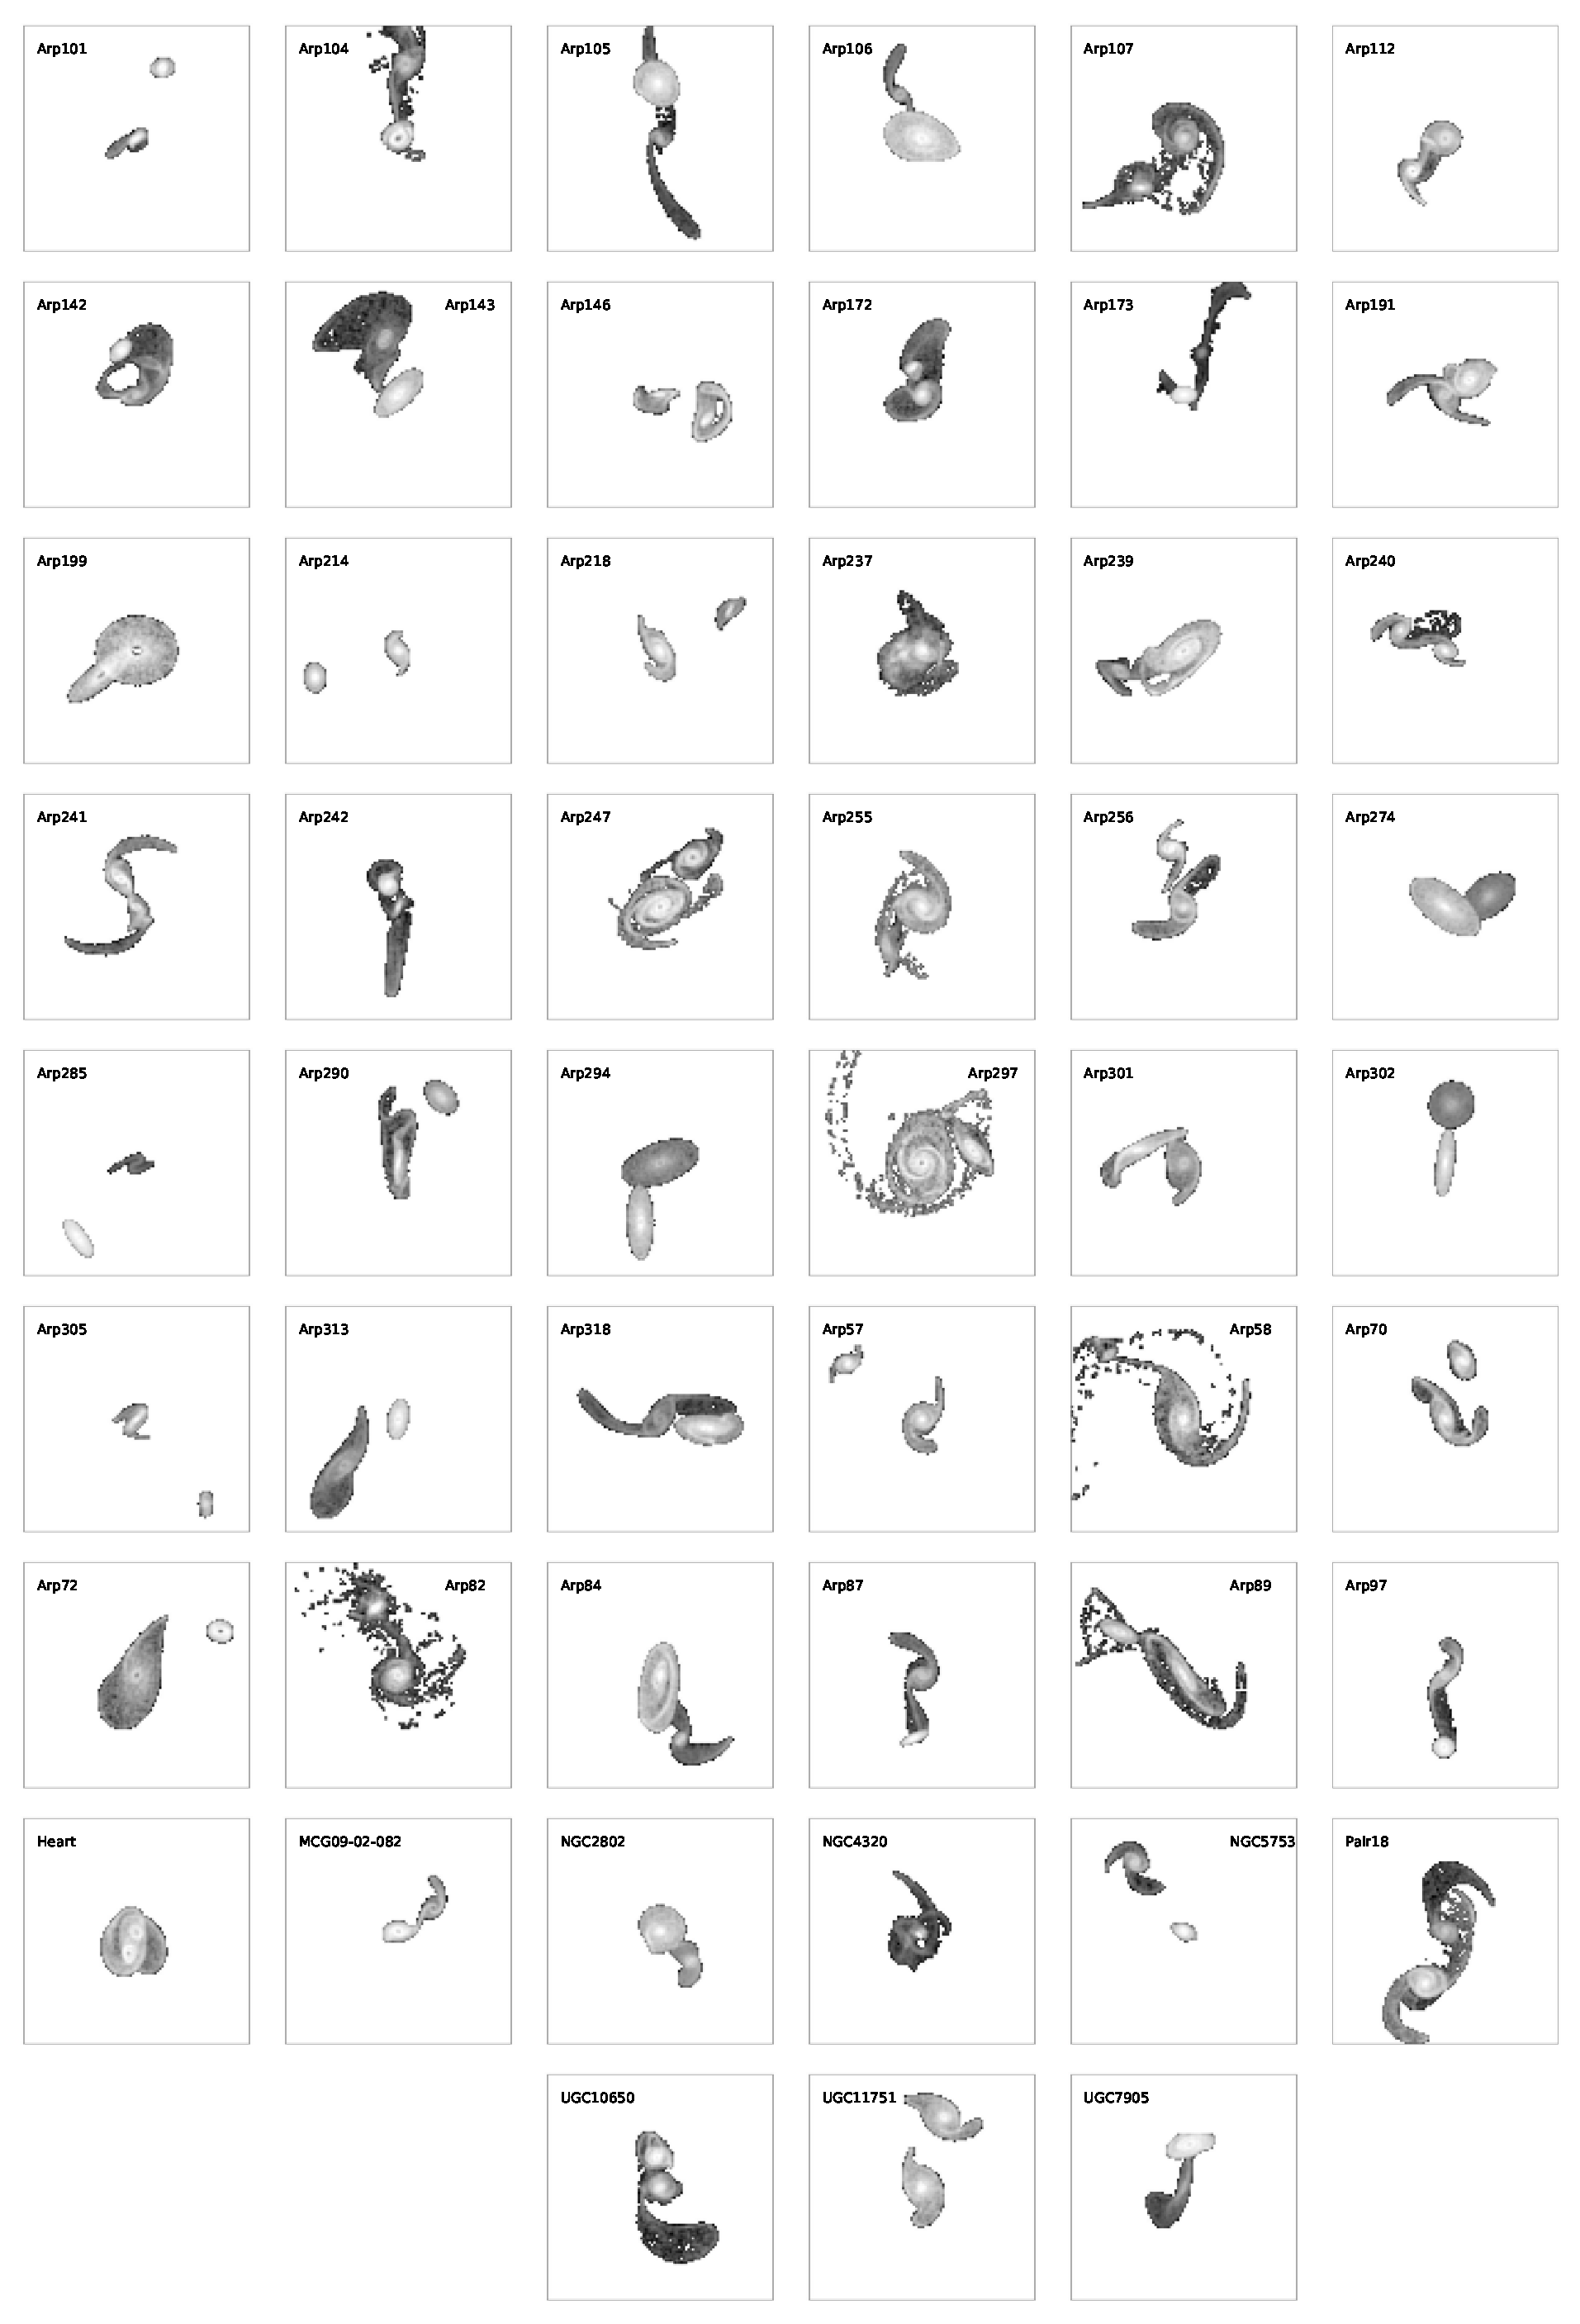
\includegraphics[width=0.90\textwidth]{Chapter1/figures/mock-images.pdf}
    \caption[Our mock observations of each interacting system.]{Our mock observations of each interacting system. These act as an idealised observation, which is completely noiseless. We also know the underlying parameters which formed these outputs. Therefore, this forms an excellent test-set to see if we can recover the underlying parameters when searching over a large parameter space.}
    \label{fig:Obj_Cutout}
\end{figure*}

\section{Constraining Interaction}\label{method:constraint}
We now require a method to compare our simulation images to our synthetic images. This comparison acts as a way to map the set of underlying parameters to an output morphology that we can then constrain by comparing to observations. However, we need a framework to conduct this comparison and to explore the parameter space of our interactions. To do this, we use an Markov-Chain Monte Carlo (MCMC) algorithm. In this section, we first describe the parameter space we explore, followed by our MCMC algorithm, how we quantify the similarity between simulation and synthetic images and how we find the parameters which are best fit.

\subsection{The Parameter Space of Interaction}
We aim to explore the underlying parameter space of interaction and find the best fit parameters which describe an input observation or test image. The parameters we constrain are the required parameters in the APySPAM three-body simulation algorithm. To function, APySPAM requires 15 different parameters. These are: the 6 positional and velocity vectors of the secondary galaxy, the total masses of both galaxies, their radius, 4 orientation parameters and the dynamical timeframe to model. We now also require the redshift measurement of the system to correctly estimate the flux distribution of the system. However, some of these parameters we can find before we begin exploring the underlying parameter space.

The first two parameters we find are the projected 2D position of the secondary from the primary. These are measured from the observational image of the system by converting between pixel and physical coordinates in the image. We take this position as the centre of the secondary disk. We also provide the redshift of the interacting system. The redshift not only directly impacts the flux distribution of the input image, but its scale and resolution. Therefore, we assume that this parameter is known and provided. Work is currently being conducted to making this a free parameter that can also be constrained based on the interacting systems flux distribution and size.

Thus, there are 13 different free parameters to recreate an interacting systems morphology and are the 13 parameters we will constrain over. A description of these parameters and the size of the parameter space explored are shown Table \ref{tab:parameters}. We choose the limits of the parameter space based on the maximum values of the parameters we used to build our test images in Table \ref{tab:Objects}. Table \ref{tab:parameters} provides the size of the parameter space as well as the conversion between the simulation units and physical units. This is primarily for reference for those who would wish to use our simulation to their own datasets. The conversions are found from \citet{1990AJ....100.1477W}.

\begin{table*}
    \centering
    \resizebox{1.00\textwidth}{!}{\begin{tabular}{|c|c|c|c|}
        \hline
        Parameter & Description & Conversion(Spec. Units) & Parameter Range(Spec. Units)  \\
        \hline
        $z$-position & Secondary $z$-position & 15kpc & -300kpc - 300kpc \\
        v$_{x}$,v$_{y}$,v$_{z}$ & Secondary velocities & 169.34kms$^{1}$ & -1693kms$^{-1}$ - 1693kms$^{-1}$ \\
        M$_{1}$,M$_{2}$ & Total Masses of Galaxy & 10$^{11}$M$_{\odot}$ & 1 $\times$ 10$^{9}$M$_{\odot}$ - 4 $\times$ 10$^{12}$M$_{\odot}$ \\
        R$_{1}$,R$_{2}$ & Radii of Galaxies & 15kpc & 0.15kpc - 150kpc\\
        $\phi_{1}$, $\phi_{2}$ & Y-axis orientation & deg & 0$^{\circ}$ - 360$^{\circ}$ \\
        $\theta_{1}$, $\theta_{2}$ & Z-axis orientation & deg & 0$^{\circ}$ - 360$^{\circ}$ \\
        t & Time of Min. Separation & 57.7Myr & 0Myr - 500Myr \\
        \hline
    \end{tabular}}
    \caption{The thirteen parameters used in both JSPAM and APySPAM to recreate an interaction. Each of these parameters must be found to consider an interaction constrained. The Parameter column shows how each parameter will be described throughout the rest of this paper. The third column then gives the conversion required to go from simulation units to SI units.}
    \label{tab:parameters}
\end{table*}

\subsection{Defining the Likelihood Function}
\subsubsection{MCMC \& Bayes Theorem}
We define framework by which to explore our parameter space, and identify areas where the parameter set successfully represent the input image. We combine APySPAM with a MCMC methodology in order to fully explore the underlying parameter space. In an MCMC, a set of walkers are created and are then moved through parameter space in an ensemble. Each walker position is a set of parameters in our 13D parameter space. At each point, we calculate the likelihood that the output simulation is representative of the input interacting system. We then compare the likelihood between the old and new position, and if the likelihood is higher at the new position the walker moves there. If not, the walker remains in place and makes another attempt to find a higher likelihood. The walkers form their own chain of steps which gradually move towards the areas of highest likelihood. In our case, the likelihood is a measurement of the similarity in flux distribution between a simulated image with parameters of the walker position and an observed image of unknown underlying parameters. Therefore, the walkers are moving from a set of underlying parameters that poorly describe the observed system to a set of underlying parameters which describe the observed system well. 

We use the well known Python package EMCEE \citep{Foreman-Mackey_13} for our MCMC. This is an ensemble MCMC package with numerous predefined moves and algorithms to make getting to the area of high likelihood more efficient. We construct contours of walker mass and use these to calculate the errors and probability distribution of our best fit measurement; i.e. we can construct a posterior for each of our parameters. For full details of EMCEE and the different modes that it can use, see the extensive readthedocs\footnote{\url{https://emcee.readthedocs.io/en/stable/}}; but here we will briefly state the hyper parameters that we use. 

For each observed image, an ensemble of six hundred walkers was initialised which would explore a total chain length of 7500 steps. Following the advice in the documentation regarding potentially complex and multi-model parameter spaces we utilised two different walker move proposals in our algorithm. These were the Differential Evolution (DE) Move \citep{Nelson_14} and the Snooker Differential Evolution (DES) Move \citep{ter_Braak_08}. An identical version of our setup can be found on GitHub\footnote{\url{https://github.com/AstroORyan}}. Here, a user can download our setup to reproduce our results, or to update the model for their own purposes.

We define a likelihood function to compare the input images to our simulation outputs. By Bayes Theorem, the probability that a set of underlying parameters which produced a simulation also describe a test image follows Equation \ref{bayes},
\begin{equation}\label{bayes}
    P(H_{i}|D_{obs},C) = P(H_{i}|C)\frac{P(D_{obs}|H_{i},C)}{P(D_{obs}|C)}).
\end{equation}
P(H$_{i}$|D$_{obs}$,C) is the probability that some hypothesised set of underlying parameters, H$_{i}$, successfully describes some observational data, D$_{obs}$, under some prior constraints, C. Applying this to our hypothesis, H$_{i}$, allows us to utilise the prior knowledge that we have about the interacting system in question and can be used to put constraints on the parameter spaces we explore to shorten computation time. This is described by the expression P(H$_{i}$|C). This is multiplied by the likelihood that the observation is defined by the hypothesised parameters given the constrains,P(D$_{obs}$|$H_{i}$,C), all divided by a normalisation constant, P(D$_{obs}$|C).

\subsubsection{Simplifying the Prior}
In order to simplify this expression, we make assumptions about the underlying parameter space to increase efficiency and simply our computations. We first assume uniform priors for each of our 13 parameters. Therefore, we define a range of parameter values that if a walker moves outwith, we set the probability immediately to zero. The ranges we allow for each parameter are specified in Table \ref{tab:parameters}. These ranges can be tweaked, or a different prior function defined, by the user. Here, we elect to set the priors part of Equation \ref{bayes} to one.

We improve efficiency in our code further by adding to the prior based on the likelihood that tidal features will form in any given interaction. This is defined by a filter parameter, $\gamma$, and is fully described in \citet[][where it is called $\beta$ but we call it $\gamma$ here to not be confused with our star formation enhancement parameter of Equation \ref{enhancement_param}]{2016MNRAS.459..720H}:
\begin{equation}\label{gamma_param}
    \gamma_{min} = \frac{M_{1} + M_{2}}{r_{min}^{2}V_{r_{min}}}.
\end{equation}
Here, $r_{min}$ is the closest approach distance, $V_{r_{min}}$ is the relative velocity at the time of closest approach and $M_{1}$ and $M_{2}$ are the primary and secondary masses, respectively. This parameter is designed to capture two important quantities: the mutual gravitational attraction and the inverse of the closest approach velocity. Each of which is important for the resultant gravitational distortion of the interacting system. By maximising the total mass of the system, while minimising the distance of closest approach and maximising the time of closest approach (i.e. minimising $V_{r_{min}}$) we would expect stronger tidal distortion. 

In our case, we use it to inform our prior as the MCMC continues. This significantly enhances the computational efficiency and pushes the walker ensemble to areas of high likelihood quickly. In each step of the MCMC, running the simulation itself is the highest computational cost, so we calculate $\gamma$ first and then make a decision on whether to run the simulation. This decision is based on an exponentially declining probability dependent on the value of $\gamma$. This probability, or prior, is defined as 
\begin{equation}\label{tidal_prob}
    C = 
    \begin{cases}
        \exp(0.5\frac{\gamma}{\gamma_{min}}), & \text{if } \gamma < 0.5 \\
        0, & \text{if } \gamma \geq 0.5
    \end{cases}
\end{equation}
Here, $\gamma$ is a user defined cutoff, 0.5 in our case. Taking the log of this, we can directly add it to prior. If the prior is initially calculated above 100, we do not run the simulation and move the walker to a new set of parameters.

\subsubsection{Simplifying the Likelihood Function}
To further simplify the likelihood function, we can assume our probability distribution is Gaussian. This is a reasonable assumption to make as a starting point for our constraining attempts. However, as will be described in section \ref{Results} this is found to not always hold true; particularly for the orientations of the system. However, making this assumption allows us to utilise the following Equation to compare our mock observations to our observed data;
\begin{equation}\label{like_gauss}
    P(D_{obs}|H_{i},C) = (2\pi\sigma^{2}_{j})\exp(-\frac{1}{2\sigma^{2}}\sum_{j=1}^{n}(x_{j}-\mu)^{2}) \times C.
\end{equation}
Here $\sigma_{j}$ is the uncertainty in the observed image, $x_{j}$ is our mock observation and $\mu$ is the observed image. The above expression can be simplified further by noting that the expression in the exponential function is just a half of the $\chi^{2}$ difference between the observational image and the mock observational image. This is the same $\chi^{2}$ function that is used in the code GALFIT \citep{2002AJ....124..266P}. Where $\chi^{2}$ is given by;
\begin{equation}\label{chi_squared}
    \chi^{2} = \frac{1}{N - n_{dof}}\sum_{0}^{N_{x}}\sum_{0}^{N_{y}}\frac{(p_{x,y} - q_{x,y})^{2}}{\sigma_{x,y}^{2}}.
\end{equation}
Here, N is the number of pixels in the observed image, which has the number of degrees of freedom subtracted from it, n$_{dof}$. $p_{x,y}$ and $q_{x,y}$ are the flux values of the (xth, yth) pixel in the observed and simulated images respectively. $\sigma_{x,y}$ is the $\sigma$ value of the (xth,yth) pixel; this is the uncertainty in the observed images pixel value and follows the $\sigma_{x,y}$-image definition from GALFIT \citep{2002AJ....124..266P,2010AJ....139.2097P}. This is then summed over all pixels in the image, giving us a single $\chi^{2}$ value between each simulated image and observed image.

Finally, to help computation time the log is taken of our likelihood function. This leaves us with a final expression that a given set of parameters describing a simulation image also describe the observed image input into the algorithm,
\begin{equation}\label{likelihood}
    \log_{10}(P(H_{i}|D_{obs},C)) = \log_{10}(L) = - \frac{\chi^{2}}{2} + \log_{10}(C).
\end{equation}
This is used at every step of our MCMC chain, with a simulation have to be run for each.

Thus, we now have a method by which to quickly predict the resultant morphology and flux distribution that the user would observe in a set of given filters. We also have a means of exploring the likely parameter space of an interaction, given an existing observation. To test this methodology, we first apply it to an idealised scenario where we know the true underlying parameters that formed the system.


\section{Results \& Discussion}\label{Results}
\noindent We now apply our MCMC algorithm to our set of synthetic interacting galaxy images. To reduce the number of repetitive figures in this paper, we focus here on a specific system as a representative sample, and publish the results of all samples online. They are presented online\footnote{All results are found here: \href{https://drive.google.com/drive/folders/1hlFhrdoZ50JaEWWYoy0RZ3J4LSoRjmsq?usp=sharing}{Link}}. As these input images are created from APySPAM, they provide us with a set of synthetic images of interacting pairs with no noise and where the underlying parameters are known. Initially, we explore the results of running this on the synthetic image of Arp 240. We discuss how the constraints could be improved, and discuss improvements on our constraints with extra, 3D information. We then plot the results for the entire dataset, and discuss trends we see in the parameters we recover.

We apply our methodology to a set of real, observed images of interacting galaxies. We select the five which are at different stages and various levels of constraint from our test dataset. We apply our MCMC to only a subset as the computational expense is significantly increased to make constraints on the observational systems and for our MCMC to reach convergence. We compare our found best fit values with those of our synthetic system, and discuss the difference between applying this to best fit simulations and observations. Finally, we describe the applicability of our approach to other systems; keeping an emphasis on those in the low surface brightness regime and the limitations this would introduce.

\subsection{Testing on a Synthetic Image}
We apply our MCMC to a single image from our mock dataset described in Section \ref{sec:syn_sample}. We elect to use this system as it is is composed of two clear and distinct disks, with a tidal bridge connecting them and tidal tails forming on the opposite side. The tidal features lie in the high surface brightness regime, and have an inclination close to 0. The observation and synthetic image are shown in Figure \ref{fig:arp240}. There are clear differences between the morphology of our mock image and the observation of Arp 240. Therefore, testing on the synthetic image is not the same as constraining the Arp 240 system. However, the synthetic image is an ideal scenario to test our methodology on. We elect to test our MCMC on the Arp 240 system first, as it has a high mass in our sample meaning the tidal features will contain more flux and should be easier for our MCMC to constrain.

\begin{figure*}
    \centering
    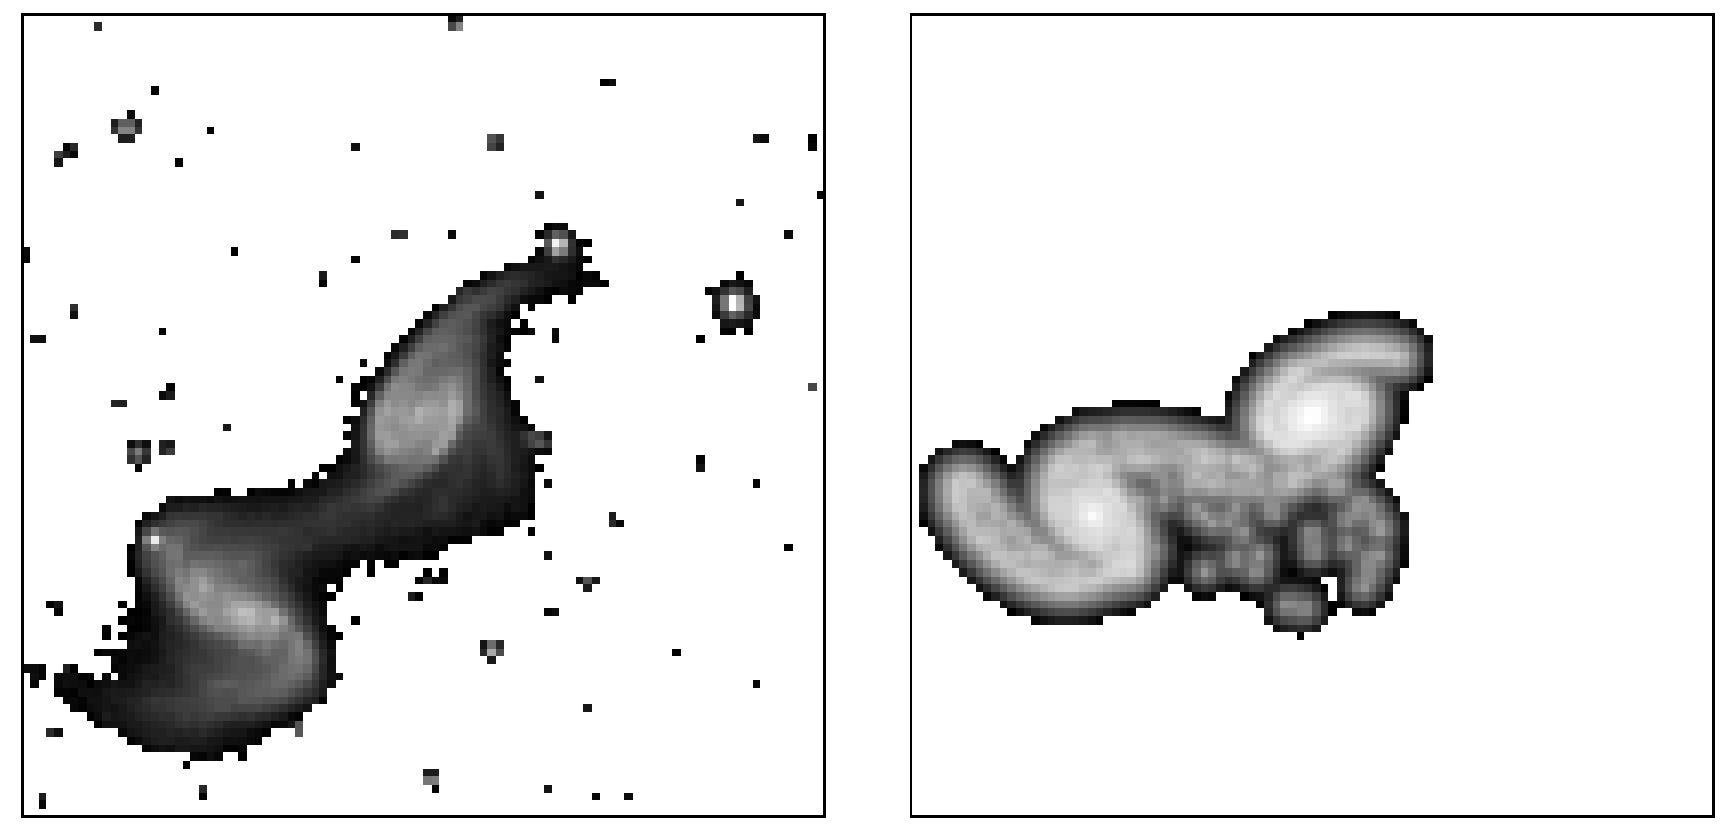
\includegraphics[width=0.75\textwidth]{Chapter1/figures/arp240-obs-sim.pdf}
    \caption[The example system used to test our MCMC: the Arp 240 interacting system.]{The example system used to test our MCMC: the Arp 240 interacting system. This system is considered an easy one to constrain. It is composed of two clearly distinct galaxies, with strong tidal features that our MCMC can match. These tidal features are the two tidal tails formed in the interaction and the tidal bridge linking the two systems. \textit{Left}: The prepared observation image of the Arp 240 system created from SDSS DR16 observations. \textit{Right}: The best fit simulation image as found by \citet{2016MNRAS.459..720H} and the first test image used in our pipeline. The different in scale and orientation are discussed below.}
    \label{fig:arp240}
\end{figure*}

We constrain the synthetic Arp 240 image by running our simulation with 2,500 particles with 600 walkers and 7,500 steps in the MCMC. An example of our full results is shown in Figure \ref{fig:corner_plot}. This corner plot is created using the Corner Python Package \citep{corner}. However, displaying our results as is shown in Figure \ref{fig:corner_plot} will be difficult as we will be discussing multiple different systems throughout this section. This larger corner plot also uses a lot of space. Therefore, we will present and discuss our results using reduced corner plots as shown in Figure \ref{fig:arp240_corner_plot}.

\begin{figure*}
    \centering
    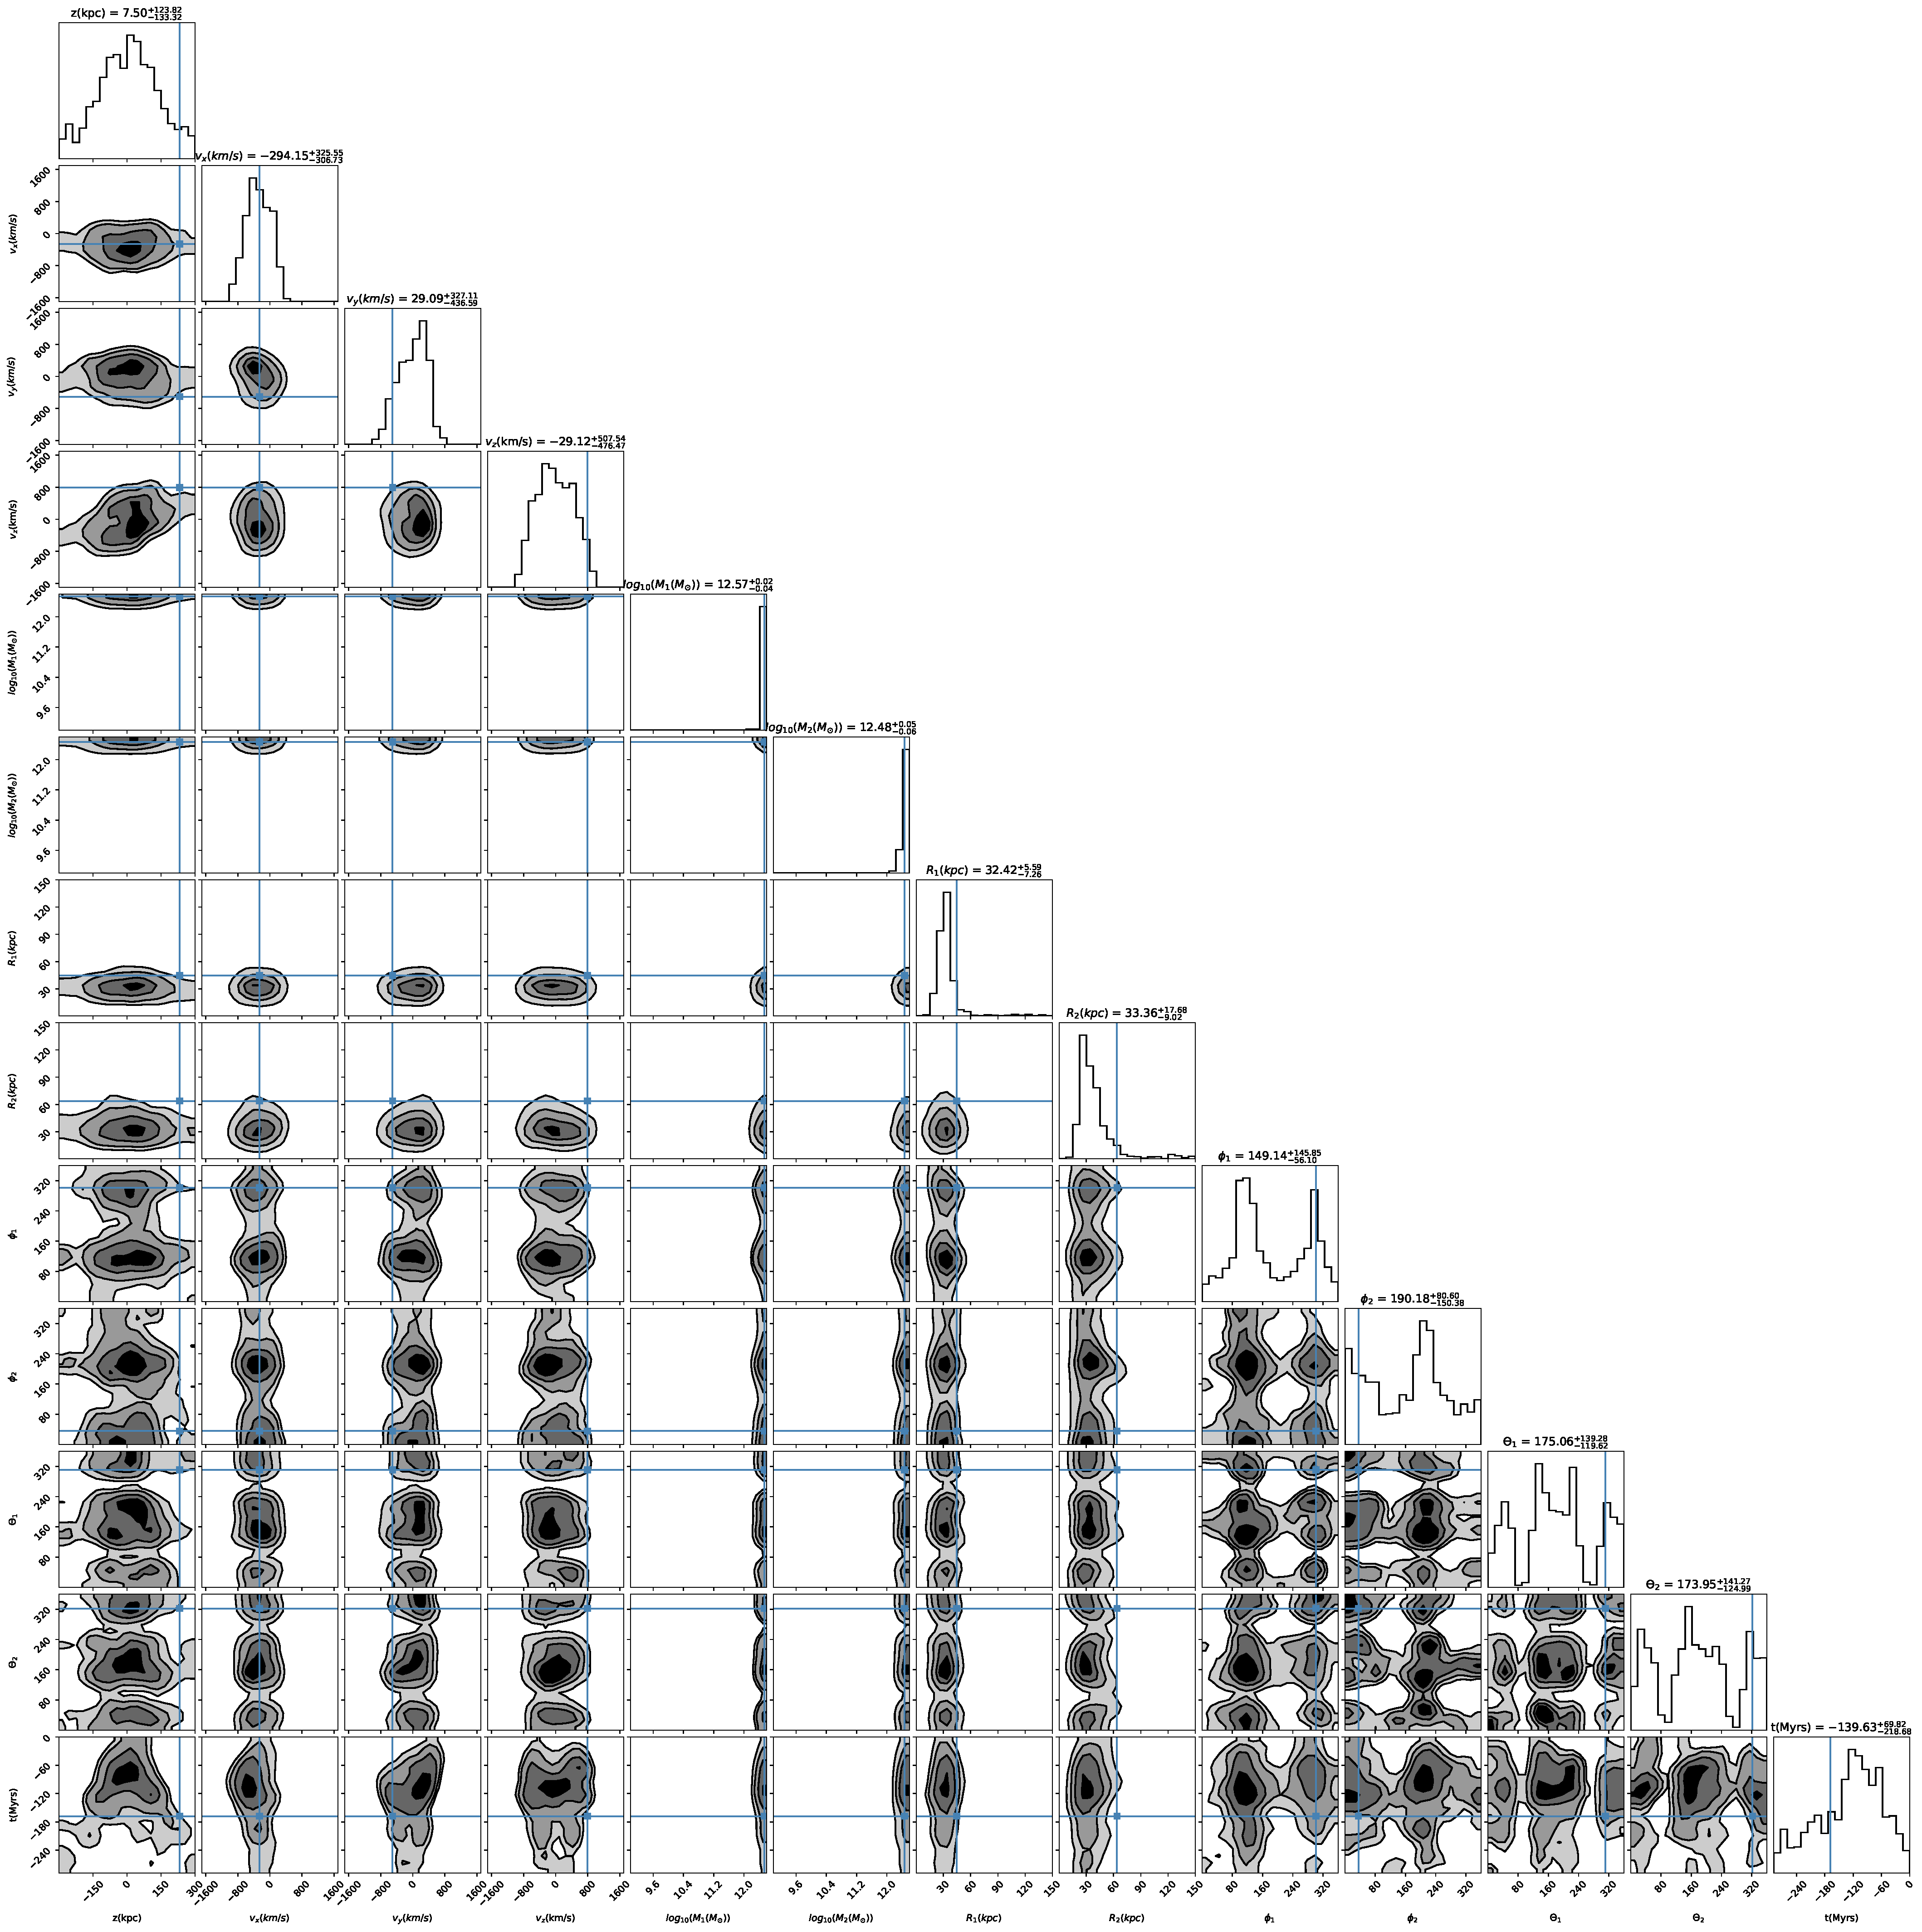
\includegraphics[width=\textwidth]{Chapter1/figures/Arp240-full-corner.pdf}
    \caption[Corner plot showing the constraints made on all thirteen parameters we are exploring.]{Corner plot showing the constraints made on all thirteen parameters we are exploring. Each contour level contains 11.8\%, 39.3\%, 67.5\% and 86.4\% of the samples across all walker chains. Displaying our results using the full corner plot is difficult in a paper because of the high dimensional results that we obtain. Therefore, we elect to show all remaining results in this paper as reduced corner plots like Figure \ref{fig:arp240_corner_plot}. We elect to put the parameters which are most likely to correlate together in different corner plots. To view the full corner plots of each system, find them at the results website for this paper.}
    \label{fig:corner_plot}
\end{figure*}

\begin{figure*}
    \centering
    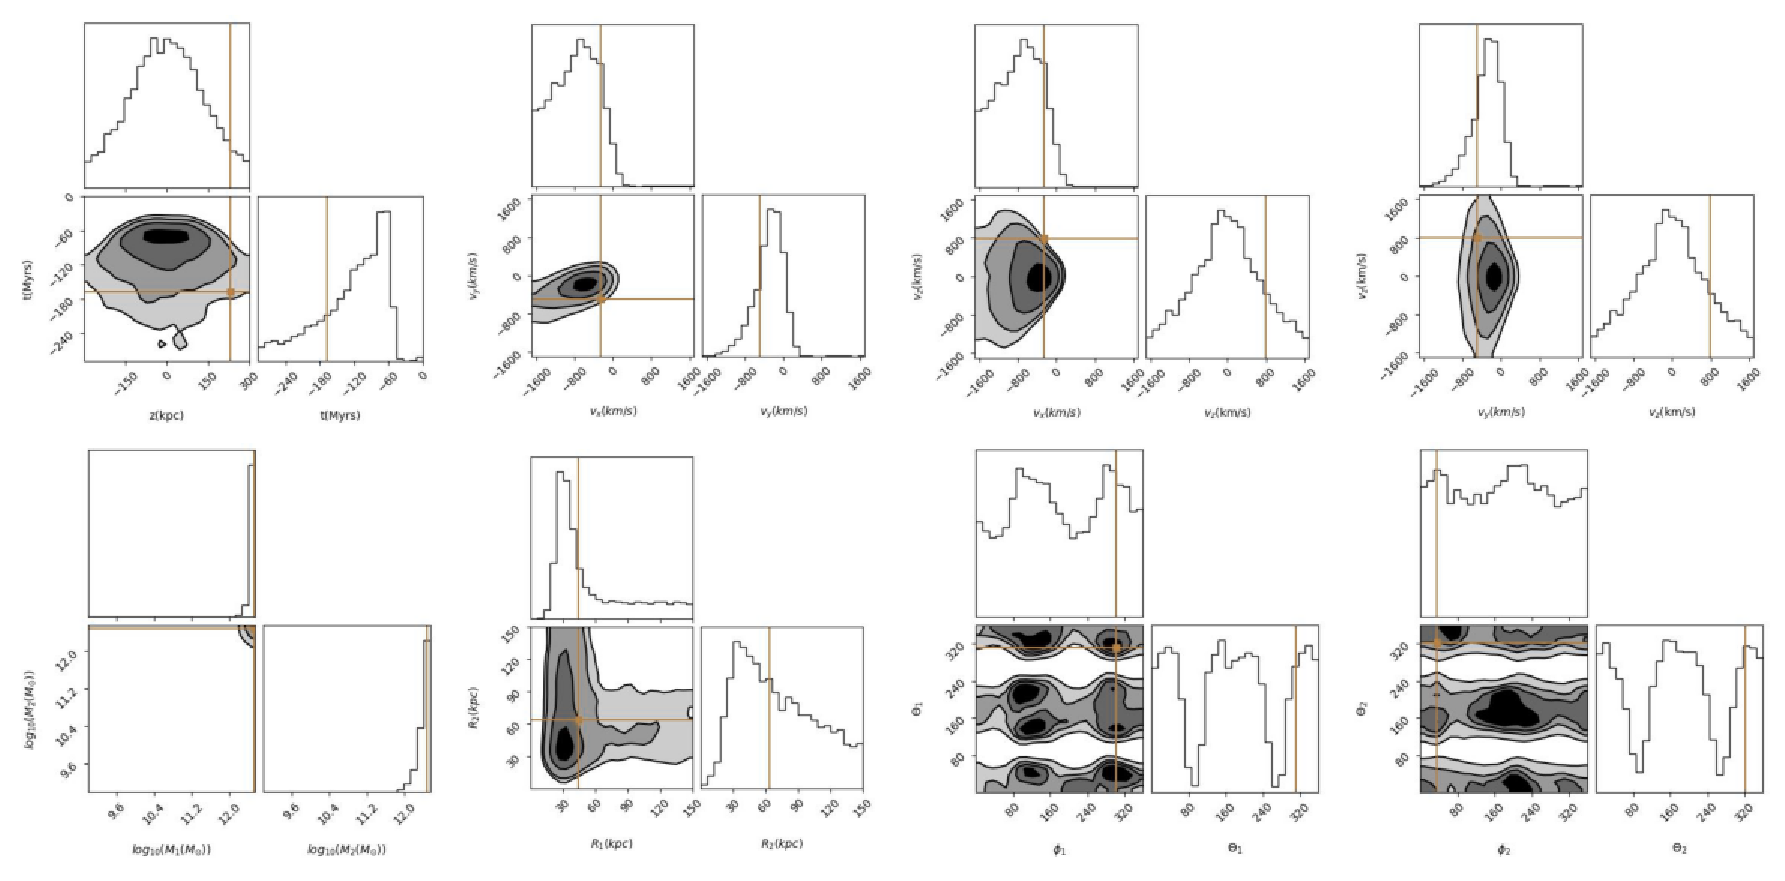
\includegraphics[width=\textwidth]{Chapter1/figures/Arp240-red-corner.pdf}
    \caption[Same as Figure \ref{fig:corner_plot}, but reduced to only corresponding parameters.]{Same as Figure \ref{fig:corner_plot}, but reduced to only corresponding parameters.}
    \label{fig:arp240_corner_plot}
\end{figure*}

% Describe the results, what are we looking at?
Figure \ref{fig:arp240_corner_plot} shows the constraints we have found on each parameter from our MCMC. The golden lines then show the true values used to create the synthetic image, and are those described in Table \ref{tab:Objects} for Arp 240. The contour levels correspond to 11.8\%, 39.3\%, 67.5\% and 86.4\% of the samples across all walker chains (these are default values), indicating the confidence level (CI). For reference, we have set up the corner plots here such that the contours containing 68\% of the walkers roughly corresponds to 1$\sigma$\footnote{Full explanation in Corner plot Docs: \url{https://corner.readthedocs.io/en/latest/pages/sigmas/}}. However, this assumes a Gaussian probability distribution, which is not strictly true for the results we find here. Figure \ref{fig:arp240_corner_plot} shows that each of the truth values is within a 67.5\% CI of the probability distribution with the exception of the $z$-position and time.

% Why do the results look like this?
We get excellent constraints on the masses of the two galaxies. This system is the most massive system in our sample, and therefore we expect the mass at the very limits of the range we are exploring. We find that the MCMC first converges on the two masses of the disks, and are the easiest for us to constrain. We provide the algorithm with the secondary 2D position, and therefore it only has to fit the flux distribution of the inner disk correctly to get good constraints on the galactic masses. The largest gains in likelihood maximisation come from matching the flux distribution in the inner parts of the primary and secondary. While the formation of the tidal features depends on the mass ratio, they also depend heavily on the orientation of the interaction as well as the relative sizes.

The relative sizes of the disks is important for the constraining the tidal features as it is the outer parts of the disk that are sheared off to form them. The primary radius is constrained very well, and is primarily expected to be smaller than the true value of this system. This is, again, due to the $\chi^{2}$ nature of calculating the distance between the two images. The likelihood, on average, is lower with some pixels within the galaxy being missed than a pixel containing the central disk in it when it should not. We therefore have a bias effect where the peak of probability drifts to just below the true value of the radius. However, the true value of the radius remains within 86.4\% CI of the found contours. 

The recovery of the radius of the secondary is worse than that of the primary. We find the peak in the probability distribution is far lower than the true value. This is from a limitation of our simulation as well. While the output simulations of the MCMC are always centred on the primary, the secondary galaxy central position is not so certain. Due to the backwards integration and trajectory calculated here, the secondary does not always end in the exact same image bin in the output simulation image. Therefore, the secondary disk likely moves slightly per simulation. This change transfers further uncertainty in the secondary disk size, and a preference for the secondary to be smaller to improve the likelihood calculation. The size of the secondary disk also contributes much more to the tidal debris formed in the interaction. The simulation is conducted in the frame of the primary, leading to the 3D velocity of the secondary being higher than that of the primary. Therefore, the particles in the secondary are much more likely to be ejected during the encounter than the simply orbiting primary particles. This adds further uncertainty to the secondary radius. However, once again, the best fit values found are within 84.6\% CI of the true value from the base simulation. 

There will also be some uncertainty involved in this measurement from the formation of the tidal features. The flux distribution of the tidal features that form are inter-dependent on multiple parameters; primarily the mass ratio, the size ratio and the orientation of the galaxies in the interaction. The significant degeneracy in the orientation constraints undoubtedly has some effect on the fitness of the resultant system. Due to a lack of three dimensional information, our algorithm cannot discern which way the galaxy is rotating or which way the tidal features should be orientated in the line-of-sight. Therefore, degeneracy at $\pm180^{\circ}$ of the true parameter values for $\phi$ and $\pm$180$^{\circ}$ for $\theta$. Figure \ref{fig:arp240_corner_plot} shows this with several different peaks in both measurements of $\phi$ and $\theta$. However, we recover the true parameters in one of the peaks of the marginalised posterior for each orientation parameter.

It is important reiterate here that $\phi$ is the orientation of the galactic disk with respect to the $y$-plane while $\theta$ is the orientation with respect to the $z$-plane. With 3-dimensional information, such as the direction of rotation of the disks or the line of sight (LOS) velocities of the tidal features, we would be able to resolve the degeneracy in the $\phi$ parameter. However, The source of the degeneracy in $\theta$ has a different source. The tidal features can form in the opposite direction from the mock observation and still be found to have high likelihood. This is a result of our likelihood being based on flux matching on pixels. There is no knowledge provided of the direction the tidal features should be moving or forming, only if the pixels contain the correct flux. Therefore, this gives a significant degeneracy in the $\theta$ parameter. Therefore, while the disk can be flipped in the $z$-direction and still match the observation, it can also be flipped in the $y$-direction as well. While the degeneracy in $\phi$ can be solved with velocity information, the $\theta$ orientation will require information on the rotation of the disk itself. Having rotational information will allow us to constrain the bulk motion within the galaxy and the direction the inner disk should be rotating as well. These two pieces of 3D information will remove the 4-fold degeneracy in each parameter.

The lack of 3D information also affects our constraints in the z-direction: the $z$-position and the $z$-velocity. As seen in Figure \ref{fig:arp240_corner_plot}, the finds the peak in the posterior distribution for both parameters as much lower than they truly are. First, the $z$-position is difficult to constrain as we lack 3D information. The simulation is run in the reference plane of the primary galaxy, therefore the secondary can only be behind or in front of iy. There will be change in the flux of the secondary based on whether it is in front or behind of the primary galaxy. However, this change in flux is completely dominated by the distance due to the redshift of the galaxy. Therefore, there is little to no observable change in the absolute values of flux unless the true value of the $z$-position was very large.

The constraint of the $z$-velocity remains far from the true parameters due to similar reasons as above. The true value lies at the very edge of the probability distribution found, at approximately 86.4\%. This would, again, be rectified readily by introducing velocity information into our constraints. The simulation works so that the secondary galaxy is always at the same x and y position that is defined by the user. Therefore, an output simulation with a positive or negative LOS velocity will have the same flux distribution. Hence, this constraint simply peaks about zero for the $z$-velocity.

Our MCMC works significantly better, however, with the $x$- and $y$-velocity of the secondary galaxy. We find the the truth value of this is within 67.8\% CI of our found distribution. The velocity values are directly related to the strength of the interaction, and therefore indirectly relate to the tidal features which form. Thus, our MCMC is informed by the flux distribution of the resultant simulated image and gives an excellent constraint on the parameters.

% Need to replace this time of interaction with the correct one. 
Finally, we discuss attempting to constrain the time of the interaction. We show the time since closest approach, not the total interaction time. The underlying simulation utilises backwards integration to calculate the trajectory of the interaction. Therefore, the time we input into the simulation simply tells it how far back in said trajectory to put the secondary galaxy. Therefore, the same interaction will occur whether we input -10 time units or -100 time units. The algorithm will require more computation time to calculate the particle positions in the lead up to the interaction. It is important to note that the total integration time will only affect the output system when we make it too small. In other words, if the secondary starts after the point of closest separation or at closest separation, our simulation breaks down and gives nonphysical results.

We calculate the time of closest approach for all of our walker steps and then present this as a measure of the time posterior distribution. Our measured value is significantly smaller than the true value of our best fit simulation, although it does lie within the region of 86.4\% CI. This parameter is highly dependent on the velocity and position constraints that we have made, and these are skewed to significantly smaller values than the truth. Therefore, it is unsurprising that our time of closest approach value is also found to be much smaller.

To fully put this result into context, we explore the simulations that lie in the areas of highest probability within these posteriors. To select which simulations to present, we take those walkers that were within the 11.8\% CI throughout each walker chain and take the top 5 as an illustration here. Our MCMC is not able to precisely reproduce the input image. It is often able to reproduce the tidal features of the primary as well as the tidal bridge connecting the two systems. This appears to be where the MCMC has centered the posterior upon. The likely reason for this is actually due to the filtering parameter that we use on the simulation. The Arp 240 simulation lies in an unlikely area of tidal features to form - $\gamma = 0.259$ - and, therefore, we update our prior to make the true result appear less likely. However, the $\gamma$ parameter remains a necessity in our MCMC. Without the ability to filter the simulations quickly, we begin to approach very large requirements of computational expense. Therefore, for this particular example the $\gamma$ parameter is a hindrance.

\begin{figure*}
    \centering
    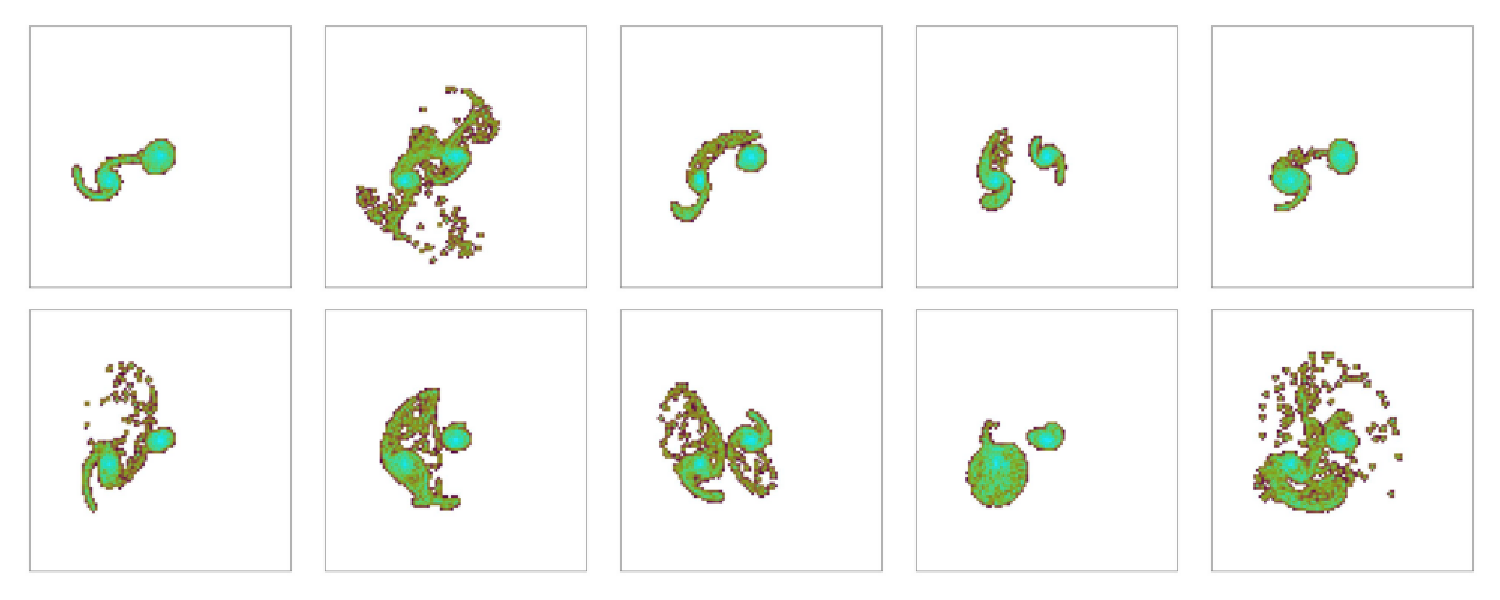
\includegraphics[width=\textwidth]{Chapter1/figures/best-fits-comb.pdf}
    \caption[Simulations from the areas of parameter space that lay within the 11.8\% CI of our constraints.]{Simulations from the areas of parameter space that lay within the 11.8\% CI of our constraints. \textit{First Row}: The synthetic image we are attempting to constrain. \textit{Second Row}: The best fit simulations from this parameter space. \textit{Bottom}: The worst fit simulations from this parameter space. Our MCMC found those parameters which cause the formation of the correct tidal features, as well as the tidal bridge connecting the two systems. However, it has been unable to fully identify the tidal features of the secondary. There is also a lot of noise in this posterior distribution, with many systems with different tidal features in the areas of high probability. Therefore, identifying specific systems with the sought after tidal features requires manual intervention.}
    \label{fig:arp240_corner_plot}
\end{figure*}

% This is likely better in the conclusion.
In the surrounding area of probability space, however, we find some interesting constraints. Changing each parameter by small amounts based on the posteriors of each parameter space leads to variation in the simulation outputs and tidal features. Due to the disks being well defined and aligned, this can often lead to them being weighted highly. Therefore, the question remains, how would one use this code to find their best fit simulation and actually make constraints using it? This algorithm is best used as an indication of where in parameter space the true parameters lie in recreating the tidal features observed in an observation. This reduces the size of parameter space to explore dramatically, and could be an indication of where to search with more accurate simulation models for true interacting galaxy parameters.

Overall, from our example of Arp 240, we are able to recover nearly all the true values of the input simulation to within an 86.4\% CI of the true parameters. The only missing parameter is the time since the flyby. There is significant degeneracy in constraining the orientations of this interaction, but this is expected. While our results appear like they have converged in the MCMC, we will also describe the diagnostics with which to prove this. 

\subsection{Diagnostics of Pipeline}
% Note, a quick section to discuss the diagnostics of the pipeline, proved it's converged etc. If I cannot get Chain Consumer working here, then I won't do this section.
\noindent It is important to ensure our results are reliable by using diagnostics to investigate the MCMC chains. We investigate three different diagnostics of our MCMC run. First, we check that they have truly converged with the Geweke diagnostic. The Geweke diagnostic is a Z-test of equality of means where the autocorrelation in the flattened samples is taken into account as the standard error is measured. We compare the means of the first 10\% and last 50\% of each chain in each parameter, and require the resultant Z-score to be $<1$ for convergence. We use the Geweke diagnostic as written in the ChainConsumer \citep{2016JOSS....1...45H} Python package. For this case, every parameter passes this convergence test, with the exception of the orientation parameters (although, this is likely the result of converging on multiple best-fit values).

Figure \ref{fig:arp240_corner_plot} clearly shows that each orientation has incredibly complex, multi-model structure in the parameter space. We have a 2- or 4-fold degeneracy in the output models due to three dimensional information not being available. This disrupts our Gewke diagnostic measure, which is looking for a single peak in parameter space. Therefore, by folding the parameter space over and only exploring over $0^{\circ}$ - $180^{\circ}$, we achieve a single peak in parameter space. These results then pass the Geweke diagnostic test.

\begin{figure}
    \centering
    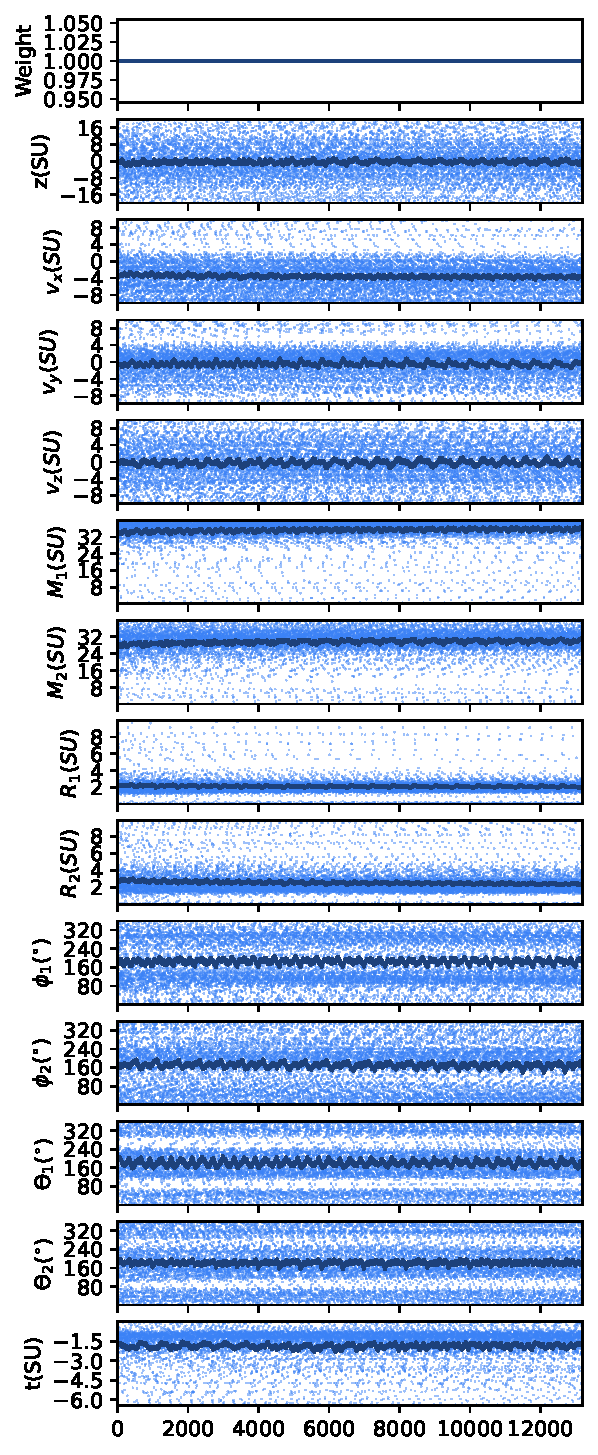
\includegraphics[width=0.45\textwidth]{Chapter1/figures/arp-240-steps.pdf}
    \caption[Steps taken by each walker in our MCMC chain to constrain the Arp 240 best fit simulation.]{Steps taken by each walker in our MCMC chain to constrain the Arp 240 best fit simulation. Note, the $y$-scales here do not extend over the full parmaeter space for some galaxies, and only show where the walkers have stepped after the burn-in phase. The deeper the blue, the more walkers have stepped at that point. This figure shows that our MCMC has successfully burnt in and very quickly goes to high areas of probability for parameter space. They then oscillate around the best fit values while searching the remaining parameter space. The $z$-position, $z$-velocity and $\phi_{2}$ parameters show dignificant uncertainty as the walkers move around the entire parameter space. In the $\phi_{1}, \theta_{1}, \theta_{2}$, we can see the two fold degeneracy form very early on and then the walkers do not explore across them at any point.}
    \label{fig:walker_steps}
\end{figure}

The second diagnostic we use is that the walkers have fully explored parameter space and that we have removed enough of the steps at the beginning of the run to consider the MCMC burnt-in. Once again, using ChainConsumer, we can plot out each walker step throughout parameter space. Figure \ref{fig:walker_steps} shows the flattened walker chains through parameter space. We have removed the first 200 steps of each walker chain before thinning the chain and flattening it. By flattening we have taken each walker chain and combined them into one chain for every parameter. Discarding the first 200 steps has been enough for the burn in of the MCMC, as the walkers have already moved mostly through parameter space and are centering on a central value of high probability. The structure in the orientation parameters is also interesting. The degeneracy structure in the parameter space has already formed by the end of the burn-in and then the walkers move within those areas of high probability. This is for two reasons. First, they affect the flux distribution of the disks primarily in if they are face-on or edge-on. The MCMC quickly converges on face-on systems in our case. Second, when they are in that degenerate space, the slight changes in inclination of the disks given does not change the likelihood calculation significantly enough to reduce this degenerate space further. Hence, the degenerate areas are very large with very flat areas of probability at their peak.

We have tested resolving this problem by running further steps in our MCMC to achieve convergence naturally within the parameter space. We find that increasing the number of steps does improve convergence on the orientation parameters, but at a much larger computational cost and without substantial improvement on the other parameters. Therefore, we elect to fold our resultant degenerate solutions into a smaller parameter space. This achieves convergence, and gives us excellent estimates on the orientation for these systems.

A second solution to this problem would be involving velocity information into our models. Knowing the bulk motion of the tidal features would allow us to constrain the tidal features based on which way they were rotating. This would eliminate part of the degenerate space. However, as stated previously, little spectroscopic data exists of our sample of interacting galaxies. Therefore, we run this test using the our synthetic Arp 240 image and including the LOS velocity of the particles and creating a velocity grid to constrain over.

\subsection{Inputting 3D Information}
Very few of the systems described in Table \ref{tab:Objects} have associated integral field spectroscopy (IFU) data in order to get LOS velocities to incorporate 3D information into our fitting process. This is because they are very large in the field-of-view of many instruments, and therefore we can only achieve measurements of their inner disks and not their tidal features. We, therefore, map the velocity distribution of our synthetic Arp 240 image. This map is created by summing the $z$-velocities of each particle in the bin and then create a total LOS velocity map for which to compare to simulations. This has little impact on the measurements of mass, size and $x$- and $y$-velocity measurements. However, it completely changes our measurements of the $z$-position and time of interaction as well as improves our constraints on all three velocity vectors dramatically. 

Figure \ref{fig:velocity_corner_plot} shows the new measurements of the constraint on the $z$-position, $y$- and $z$- velocities. The constraints on each of these parameters is significantly improved. This is with the same number of MCMC walkers and steps as without 3D information. For the $y$- and $z$-velocities, the constraints are improved to the point where we completely recover the true underlying parameter values within 39.3\% CI. With the $z$-position, we also gain significant constraint. We are able to recover which side of the primary the secondary lies, with a sharp drop in the marginalised posterior over the negative part of the $z$-position parameter space. We also significantly improve our constraint on the time of the interaction, and approximately recover the true parameter. We are able to constrain the final velocity expected in the observation, and therefore, means the galaxy cannot be moving too fast at in the final timestep. This has the effect of shifting the expected time of contact back significantly.

\begin{figure*}
    \centering
    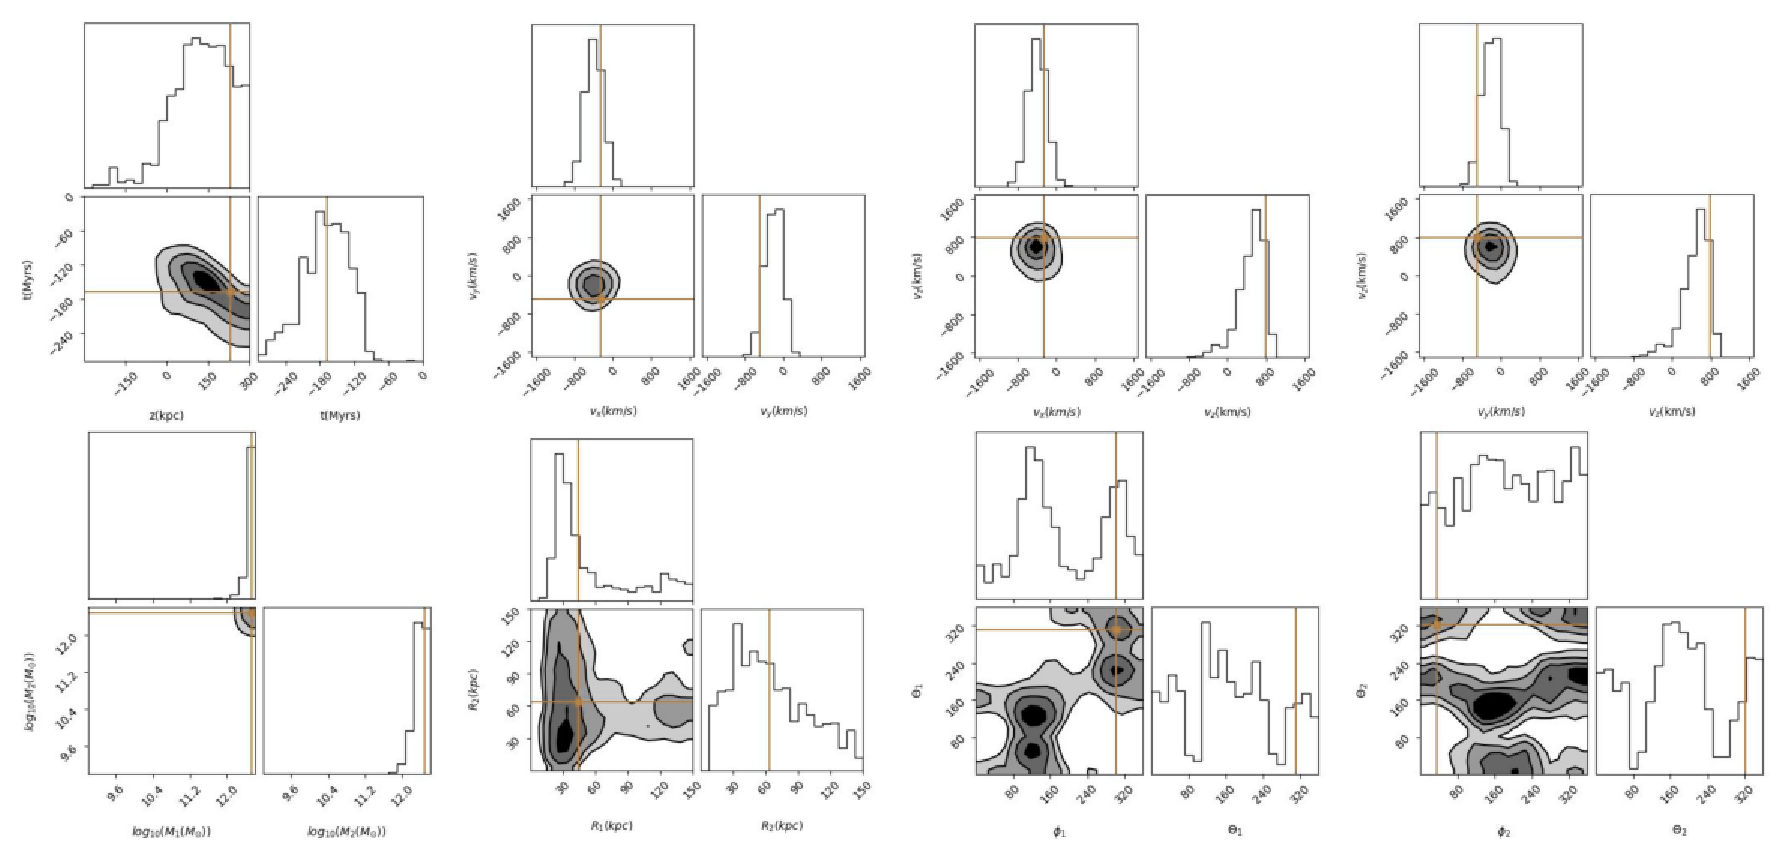
\includegraphics[width=0.9\textwidth]{Chapter1/figures/Arp240_vel-red-corner.pdf}
    \caption[The reduced corner plot of the synthetic Arp 240 system with a velocity map also used for constrained.]{The reduced corner plot of the synthetic Arp 240 system with a velocity map also used for constrained. To add this extra information, we created a mock velocity map of our Arp 240 synthetic image and summed the LOS velocity ($z$-velocity) in each pixel of our image. Comparing between here and Figure \ref{fig:arp240_corner_plot}, we see we make different constraints on the $z$-position and the time as well as resolve one of the degeneracys in the orientation space.}
    \label{fig:velocity_corner_plot}
\end{figure*}

Interestingly, we lose a significant amount of constraint on the relative sizes of the two systems. Adding the velocity information in the way we have likely increases the required size of the disks so the LOS velocities match within them. Therefore, more particles are stripped from the secondary galaxy and cause further uncertainty in the final image. We also find the removal of some of the degeneracy in the orientation parameters, as expected. It is important to note that, in this example, we have only used the LOS velocities to achieve this improvement in constraint. To better get constraint on orientation, we likely need further velocity and 3D information of the system. For instance estimates of the internal rotation, and accurate measures of the bulk motion of the tidal features in the galaxy. Currently, the simulation is not able to accurately reproduce this outwith simply assuming circular velocities at different radii from each galactic centre. Finally, the mass constraints remain the same as was found without velocity information as they are dependent primarily on the flux distribution and dominated by the inner disk of the system.


This shows the improvement that adding velocity information to our MCMC could bring, and how far interacting galaxy simulation and constraint can go once we incorporate IFU spectroscopy over more systems. In the sample we are using here, of the most massive, large, major interacting systems, only three have got any IFU data. This data is from the MaNGA \citep{2015ApJ...798....7B} IFU spectrograph, whose field of view is only able to capture the central disk of these systems. While having velocity information on even a subset of the pixels of the galaxy would improve constraints, to significantly improve them we will need this of the full tidal features of the systems. IFUs with larger fields of view are soon to come online, such as WEAVE \citep{2014SPIE.9147E..0LD}. 

\subsection{Running on Full Idealised Sample}
% Remember, this section is meant to be an overview of all of the results and simply a discussion on what we notice of applying it to different systems. This is not another deep dive like we did in the testing on one system. 
\noindent With constraints being ascertained on nearly all parameters of our synthetic Arp 240 image, we then applied our MCMC to the remaining 50 synthetic images. The reader is invited to see the resultant corner and reduced corner plots of each system on the website. Here, we will detail describe our best and worst three corner plots, and then discuss the trends throughout applying the MCMC to the dataset. First, our ability to constrain is highly dependent upon the stage of interaction. Our tightest constraints, the ones with narrowest posteriors, were on those interacting galaxies which were only just past the point of closest approach. I.e., they were the systems which had highly distinct tidal features and disks were fully separate. Our best three fits were those of synthetic images of Arp 172, Arp 240 and Arp 290. The `best fits' have been judged by those with the smallest FWHM of their marginalised probability distribution in mass. The reduced corner plots are shown in here in Figures \ref{fig:arp240_corner_plot}, \ref{fig:best-Arp172} and \ref{fig:best-Arp290}. Each of these systems is clearly in stage 2 or 3 of the interaction, where tidal features have formed clearly, and there are two distinct disks.

\begin{figure*}
    \centering
    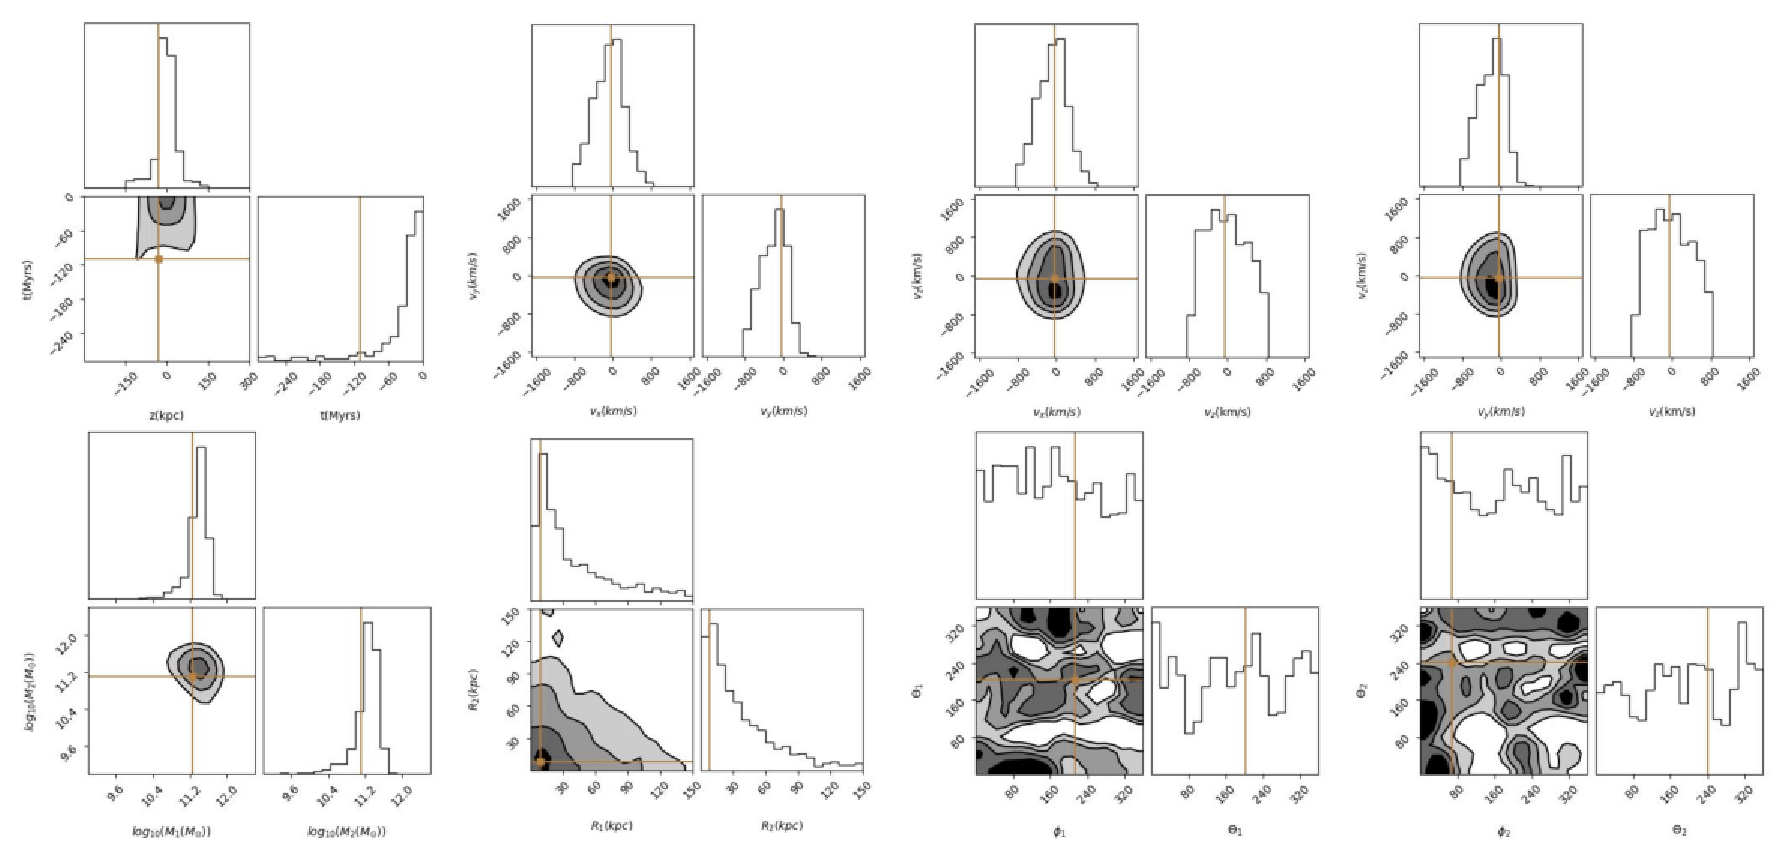
\includegraphics[width=\textwidth]{Chapter1/figures/Arp172-red-corner.pdf}
    \caption[Second example of our best fits from our methodology is representative of the simulated image of Arp 172, a stage 3 system.]{Second example of our best fits from our methodology is representative of the simulated image of Arp 172, a stage 3 system. Gold lines represent the true values.}
    \label{fig:best-Arp172}
\end{figure*}

\begin{figure*}
    \centering
    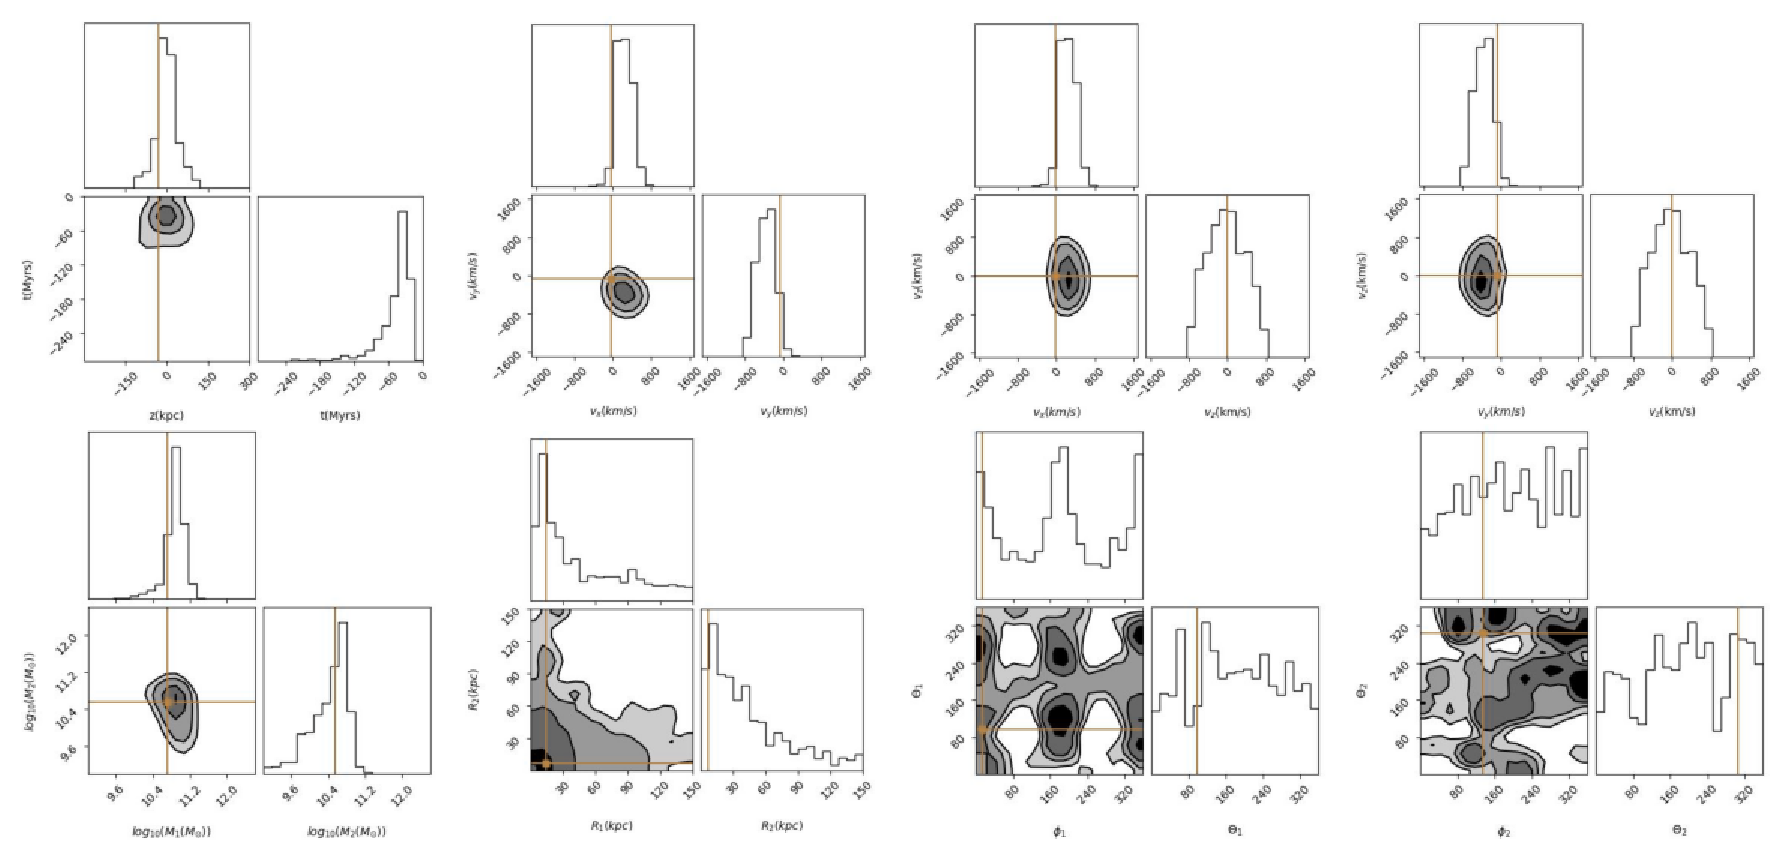
\includegraphics[width=\textwidth]{Chapter1/figures/Arp290-red-corner.pdf}
    \caption[Third example of our best fits from our methodology is representative of the simulated image of Arp 290, a stage 2 system.]{Third example of our best fits from our methodology is representative of the simulated image of Arp 290, a stage 2 system.}
    \label{fig:best-Arp290}
\end{figure*}

\begin{figure*}
    \centering
    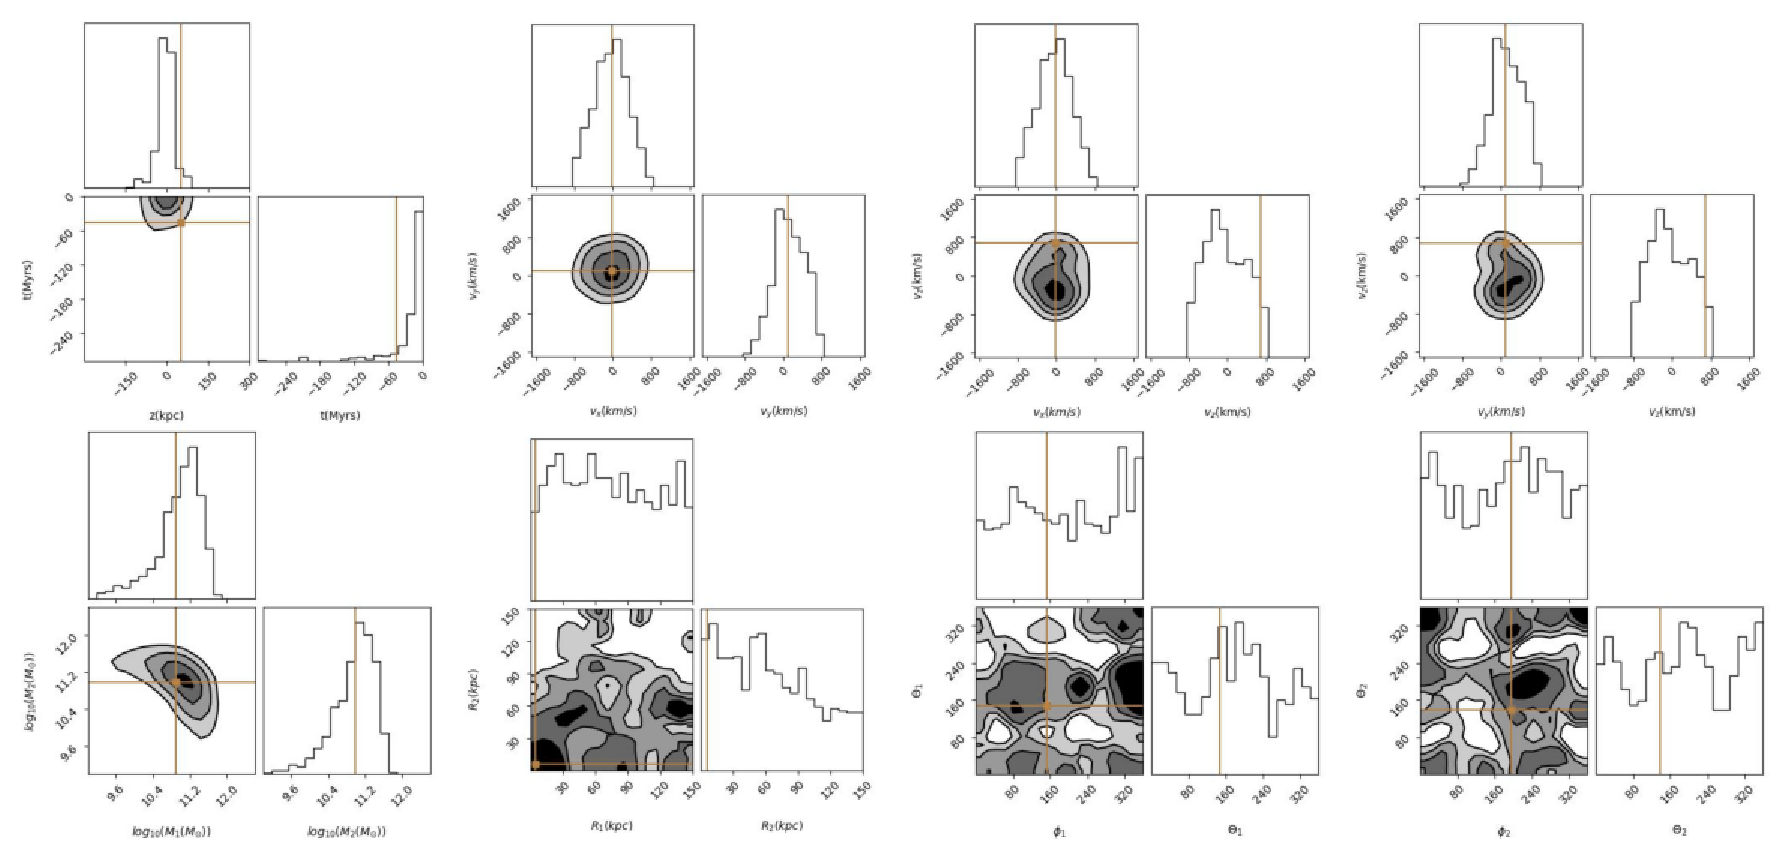
\includegraphics[width=\textwidth]{Chapter1/figures/Heart-red-corner.pdf}
    \caption[First example of our worst fits.]{First example of our worst fits. This shows our constraints of the simulated image of the Heart system, a stage 4 system.}
    \label{fig:worst-Heart}
\end{figure*}

\begin{figure*}
    \centering
    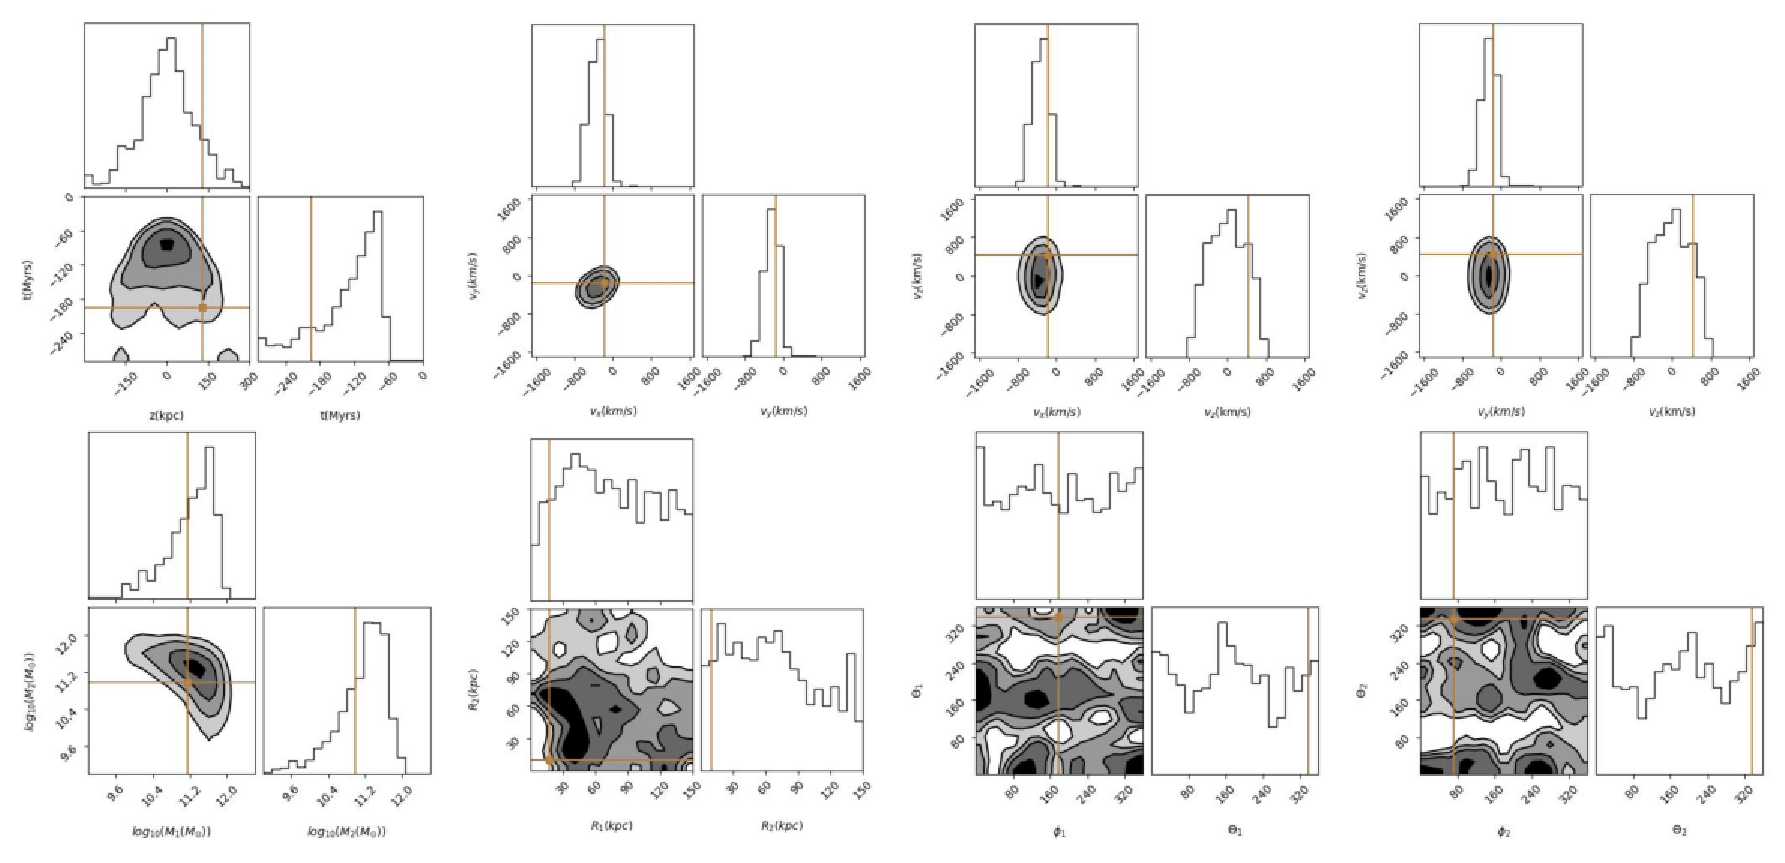
\includegraphics[width=\textwidth]{Chapter1/figures/Arp57-red-corner.pdf}
    \caption[Second example of our worst fits.]{Second example of our worst fits. This shows our constraints on the simulated image of NGC 4320, a stage 4 system.}
    \label{fig:worst-Arp57}
\end{figure*}

\begin{figure*}
    \centering
    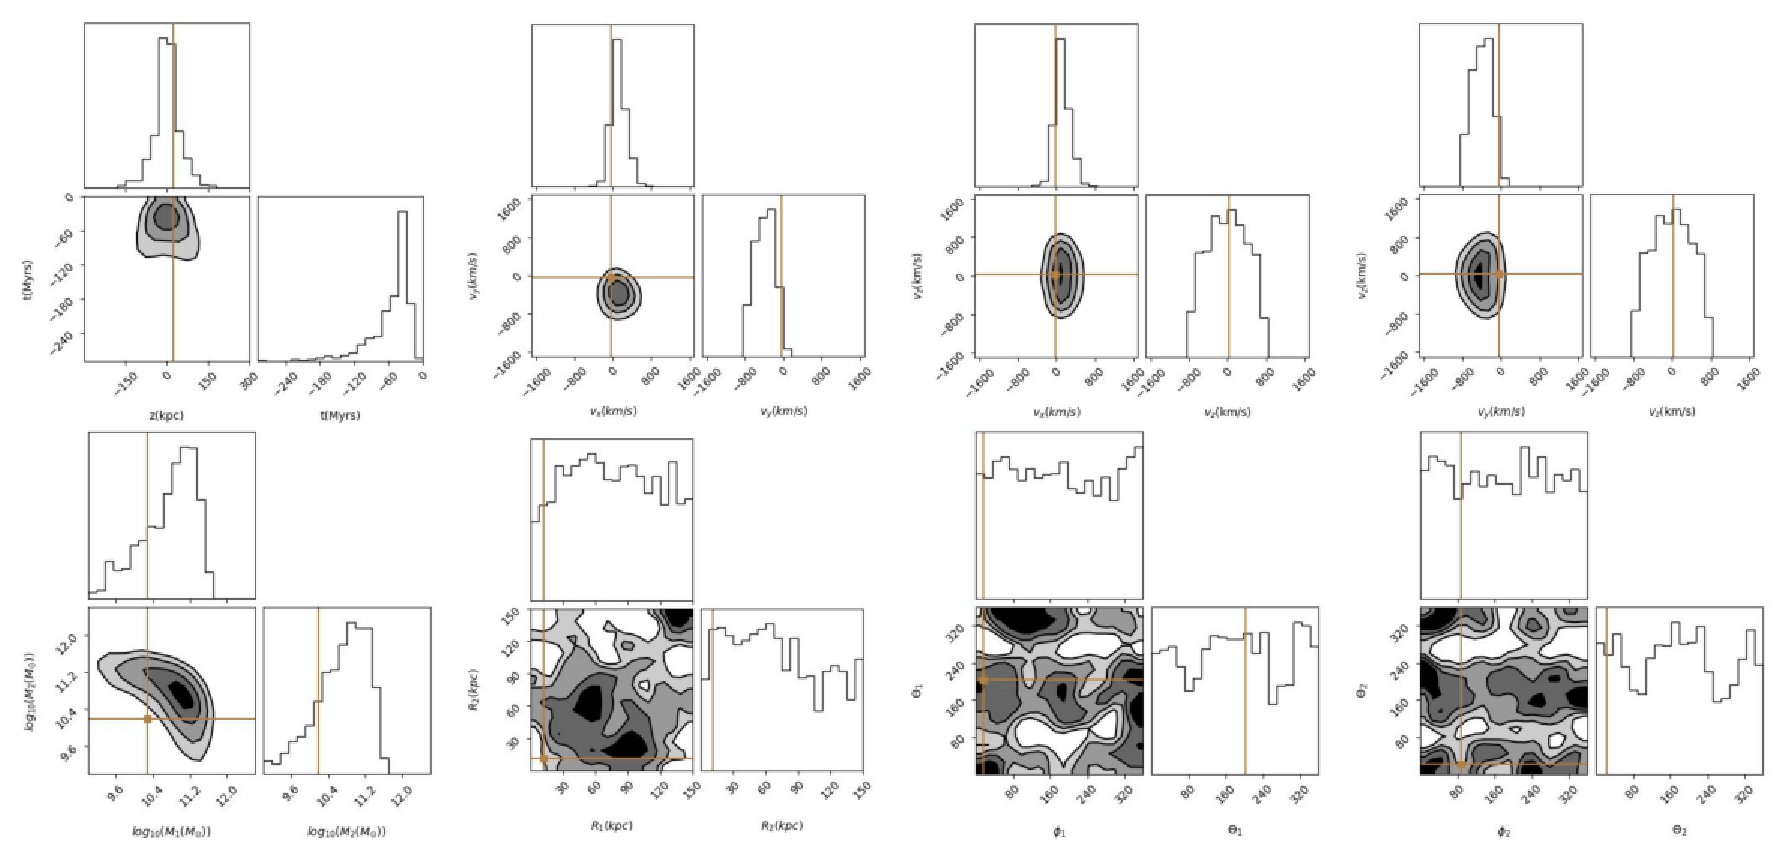
\includegraphics[width=\textwidth]{Chapter1/figures/UGC11751-red-corner.pdf}
    \caption[Third example of our worst fits.]{Third example of our worst fits. This shows our constraints on the simulated image of UGC 11751, a stage 3 system.}
    \label{fig:worst-UGC11751}
\end{figure*}

The worst fits we achieved were of those systems which were close to the merging stage. They were systems where the two cores were close to coalescence, very little tidal features were visible or the position of the secondary galaxy was very unclear. Our worst three fits and examples of this were Heart, NGC4320 and Arp 57. The reduced corner plots are shown in Figures \ref{fig:worst-Heart}, \ref{fig:worst-Arp57} and \ref{fig:worst-UGC11751}. Each of these systems represent the three limitations, respectively. First, is the issue with constraining a stage 4 system. If two cores are close to coalescence, the flux distribution will appear similar to two overlapping disks. Therefore, our $\chi^{2}$ calculation will lead to a maximised likelihood which is equivalent between systems with little to no interaction and a merger with multiple flybys undergoing coalescence. This would be improved by including velocity information, where the velocity distribution will be very different between two overlapping disks and coalescing galaxies. Our process is also not yet designed to account for multiple flybys, which is likely to have occurred in a merging system. To make accurate constraints on many parameters, we require clear and distinct tidal features. UGC 11751 is a system where we have reduced the resolution so much that we lose spatial resolution in the flux distribution of the tidal features. Therefore, we insert a significantly higher uncertainty into our constraints. Finally, our MCMC requires a secondary galaxy to make reasonable constraints on the underlying parameters. The example of NGC 4320 is a final stage merger where a large tidal feature has formed as a result of the coalescence.

% Now, going to break down the generals about each parameter space.
Throughout every system we put constraint on, the parameter we are able to get reliable constraints on are the masses of the systems. This is shown above as even our worst fit systems still hold excellent constraints, with the values confined to small areas of parameter space. However, our worst constraints lie in the orientation and time since the interaction. We show the relation between the true parameter used to create the synthetic image and our recovered best fit parameter with errors included. Figure \ref{fig:true-found-parameters} shows this distribution. We define the best fit value from our MCMC as the 50th percentile of our walker distribution. This is represented by each point in Figure \ref{fig:true-found-parameters}. The upper and lower error bars are calculated from the difference between the 50th percentile value and the 84th and 16th percentile values, respectively. The red lines in each subplot represent a 1-to-1 relation between the true parameter value and the recovered value. 

\begin{figure*}
    \centering
    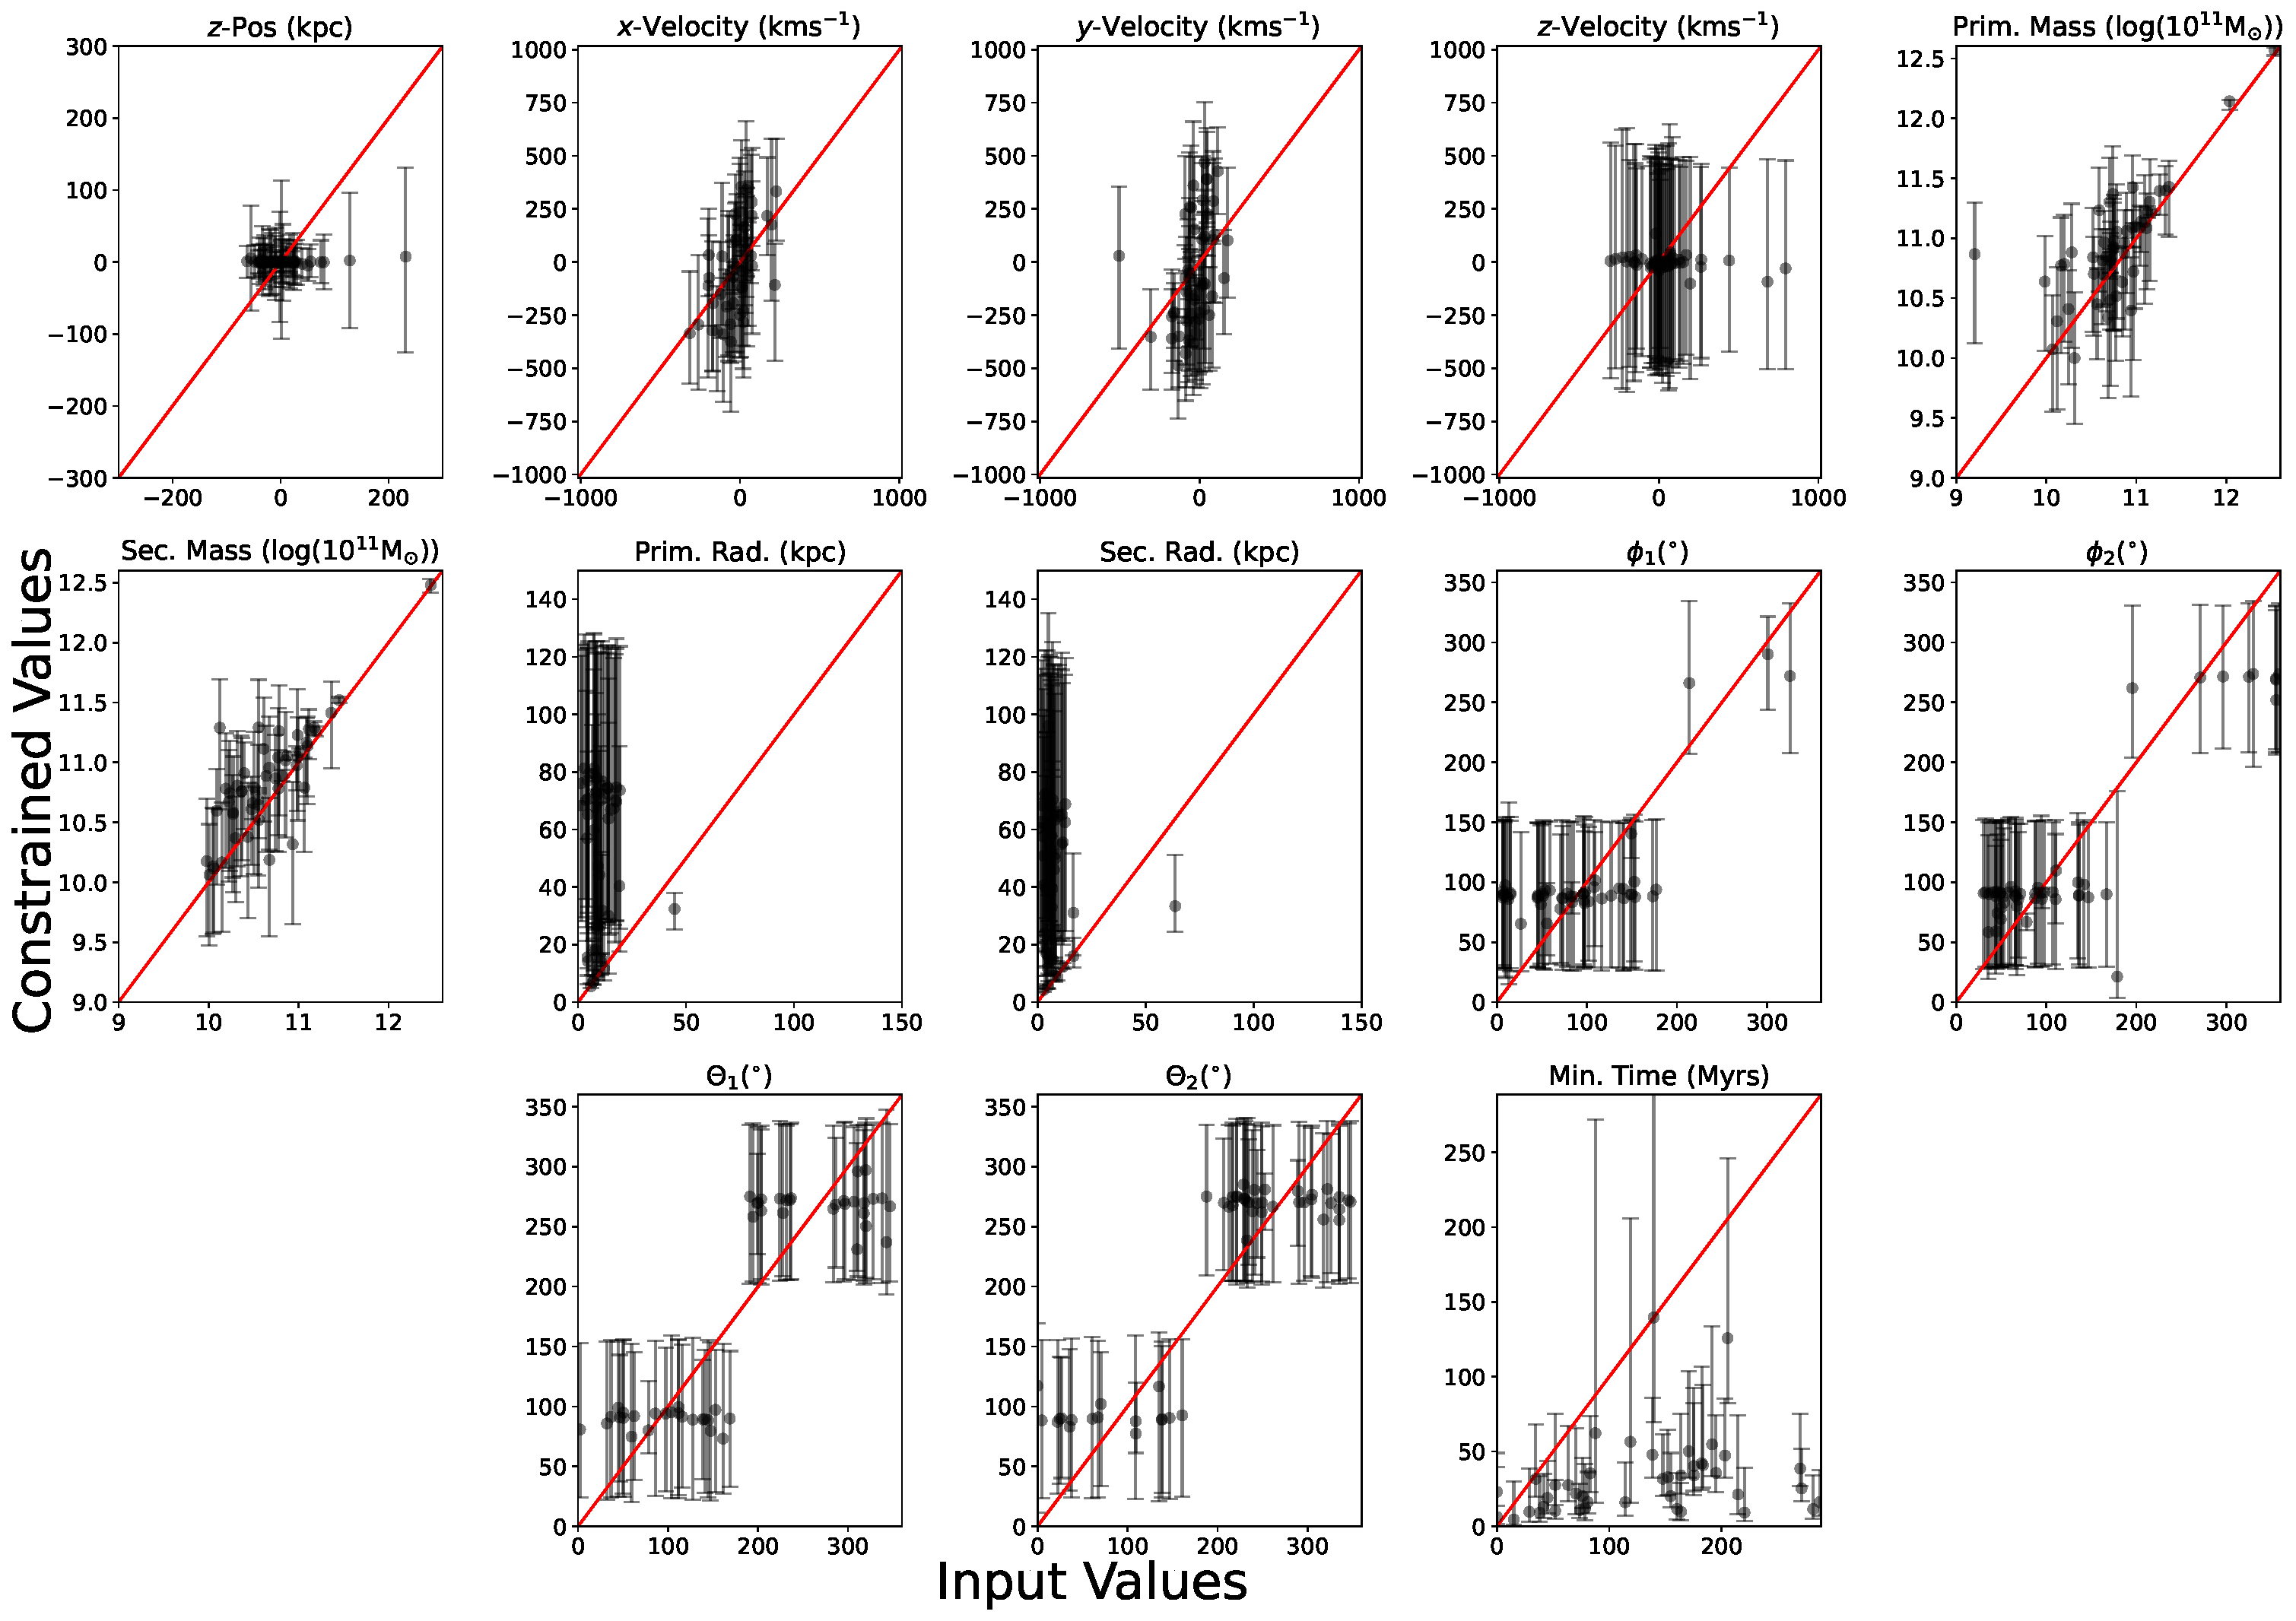
\includegraphics[width=\textwidth]{Chapter1/figures/51_51.pdf}
    \caption[The distribution of parameter values used to create our synthetic interaction images and the best-fit values we recover from our algorithm.]{The distribution of parameter values used to create our synthetic interaction images and the best-fit values we recover from our algorithm. The constrained values are taken as the 50th percentile of our walker distribution. Our lower and upper errors are then calculated as the difference from our best found value and the 16th and 84th percentiles, respectively. This gives an idea of the extent of our walker distribution in 1D. The red lines show a 1-1 relation and where our points would lie if the 50th percentile represented the exact input value found. Parameter names and unts are found in the title of each subplot.}
    \label{fig:true-found-parameters}
\end{figure*}

% Here, discuss Figure 13 in all its glory.
Figure \ref{fig:true-found-parameters} clearly shows where our MCMC has made excellent constraints and where it has not. The best constraints are on the masses of the interacting systems, where each best-fit value approximately follow the 1-to-1 relation. Where there is some discrepancy, the true values are within our errors. There is a trend here, however, that the total mass of the system is over estimated when compared to the true value. We also find excellent constraints on the majority of the positional and velocity vectors of the interaction, where the 50th percentile value approximates the true value. However, in these parameters we have explored a very wide parameter space when the majority of the true values are clustered around the centre of the parameter space. We will require further investigation with interacting systems more representative of the full parameter space we have explored. 

We also have reasonable constraints on our orientation parameters. As we often have two areas of high probability due to degeneracy, we opt to only plot the 50th percentile and errors of the high probability space near the input value. This would not be possible with an observational system with unknown parameters. Therefore, the user will either need to make a choice of what area of parameter space to explore, or input some prior on the orientation / inclination of the system. Once we have accounted for the degeneracy, we find that our 50th percentile value is representative of the true value, with the true value being within error of it. 

There are three parameters remaining where we find poor constraints or struggle to recover the true parameter value in general. The first are the radii of the two galaxies. We find that these are often over-estimated. Upon inspection of many of the output simulations, we find this is likely an effect of the distribution of particles and that we are using idealised synthetic images with no noise in the image. The way in which the particles are distributed is with an exponentially declining disk. This is achieved by creating a disk of particles which are sectioned into rings. Each ring has an exponentially declining probability of particles appearing within it based on the radius from the centre. Therefore, we find the outer rings of the galaxy are diffuse of particles, and do not dominate the likelihood function at high radius. This, in turn, means that galaxies with large angular size can be calculated as likely if the inner parts of the galaxy, with high particle numbers, match the flux of the inner disk. This also explains the over-estimate of the mass of each system. There are likely less particles than expected still within the galactic disk, and therefore more mass (ergo, luminosity) is required to keep the flux matched in the disk.

We also find we often under-estimate the time since the closest point of the encounter - i.e., the time of the passage - by a large margin. While those synthetic images whose underlying parameters had their point of passage very recently we recover very well, those at larger values we fail to. This is due to the likelihood function finding equivalent, high probability values between systems with correct tidal features and simple disks which match the inner disk of the interacting system. The former, tidal feature formation, requires a high $\beta$ parameter with low velocity and low impact distance. However, if the system is fast and does not form tidal features, but ends the simulation in the right place with the correct flux, the calculation will be dominated by the inner disk. Thus, we find a radius that covers the inner parts of the galactic disk successfully, with little disturbance that matches the flux of a large part of the galaxy. Therefore, the $\beta$ parameter is of the utmost importance to filter out these galaxies and give weight to higher t$_{\mathrm{min}}$ values.

Aside from the points that have already been raised regarding our MCMC constraining each parameter, a further problem was that the likelihood calculation is dominated by contributions from the mass and velocity parameters. Therefore, to continue improvements on other parameters further walkers and a longer chain must be run, incurring a cost of far more computation time. For the purposes of this work, we show the full degeneracy, limitations and difficulties of our model and what is to be expected in the most general case. Many of these limitations and problems can be resolved from tighter priors with more information regarding the systems being investigated.

The true power of this approach will be when investigating large populations of interacting galaxies and combining and marginalising over many different posteriors. When combining the parameter spaces of many different systems, it will be possible to identify those areas of parameter space which lead to the formation of certain features across populations of interacting galaxies. Our method will allow more intense simulations to sample smaller parameter spaces and be more efficient when finding systems with specific features. However, how to combine the posteriors is somewhat up for debate. We have ensured that the parameter spaces we are exploring are equivalent in size and that the prior is equal across parameter space. This introduces the question of the $\beta$ parameter in filtering simulations which, indirectly, changes the prior based on the trajectory of the interacting system. To conduct this combination, we would recommend that the $\beta$ parameter was not utilised when building the different posteriors if the increased computational cost is viable.

However, all of our results so far have been in the best-case scenario of a noiseless best fit simulation. The translation from simulation to observation in previous algorithms such as these is never an easy one. We, therefore, use our top three best fit systems here (Arp 172, Arp 240 and Arp 290) and apply our pipeline to their reduced observations.

\subsection{Applying to Observations}
% Brief re-iteration of creating observations.
\noindent We apply our MCMC to the reduced observational data of Arp 172, Arp 240, Arp 256, Arp 290 and Heart. Cutouts were created as described in Section \ref{data:obs-prep}. We reiterate here that the cutout resolution is reduced from its native resolution to cutouts of 100 $\times$ 100 pixels. Before we input the images into the pipeline, we find the central pixel of the secondary galaxy and convert this into a physical $x$- and $y$-position. We also find the total size physical size of the cutout in kpc, convert it to simulation units and provide this to the pipeline. We find that the physical size of the cutouts are significantly different from those of our synthetic dataset. As an example, we create the cutout of Arp 240 at 600 $\times$ 600 pixels at native resolution. With SDSS data, this corresponds to a physical size of 111.50kpc $\times$ 111.50kpc at the redshift of Arp 240. The synthetic image we previously used of Arp 240 is 785.35kpc $\times$ 785.35kpc. Figure \ref{fig:arp240} clearly shows a very different scaling between the observation and simulation, however, it is not enough to be seven times zoomed in on the system. We also find that the secondary positions are very different between the observation image and that used previously. As a result, the parameters we will find for constraining the observation will likely be very different. 

% Why do we take significantly longer on these?
We apply our MCMC to those outputs which had varying constraint. We only investigate these five systems as we find the computational expense is significantly higher when constraining the observations compared to the best fit simulations. We find the reasons for these are two fold. First, we must run each walker for twice the number of steps than when constraining the synthetic images to reach convergence. This is from increased noise contributions in the observation images. Second, due to the smaller scale size of our images, the defined $\gamma$ parameter is much stronger than with the synthetic images. Both of these reasons for higher computational expense are to be expected. The increase in the $\gamma$ parameter leads to us filtering out less candidate systems and running the base simulation code more often. This directly translates into a higher runtime for our MCMC.

% What do we find immediately?
Figure \ref{fig:obs_corner_plot} shows the reduced corner plot for the observed Arp 240 system. The constraints on the velocity parameter have significantly worsened when compared to the constrains on the best fit simulation. They are also in a different area of parameter space when compared. The velocity and spatial parameters are the most likely to be affected by the change in scale between the two input images. As the secondary galaxy position has been completely altered the best fit trajectory of the interaction has also completely changed. The secondary is significantly closer to the primary, therefore meaning the secondary velocity must be significantly slower than previously. Due to the increase in noise in the observational image, and the extent of the tidal features of the primary and secondary galaxies, the constraint has also significantly weakened.

\begin{figure*}
    \centering
    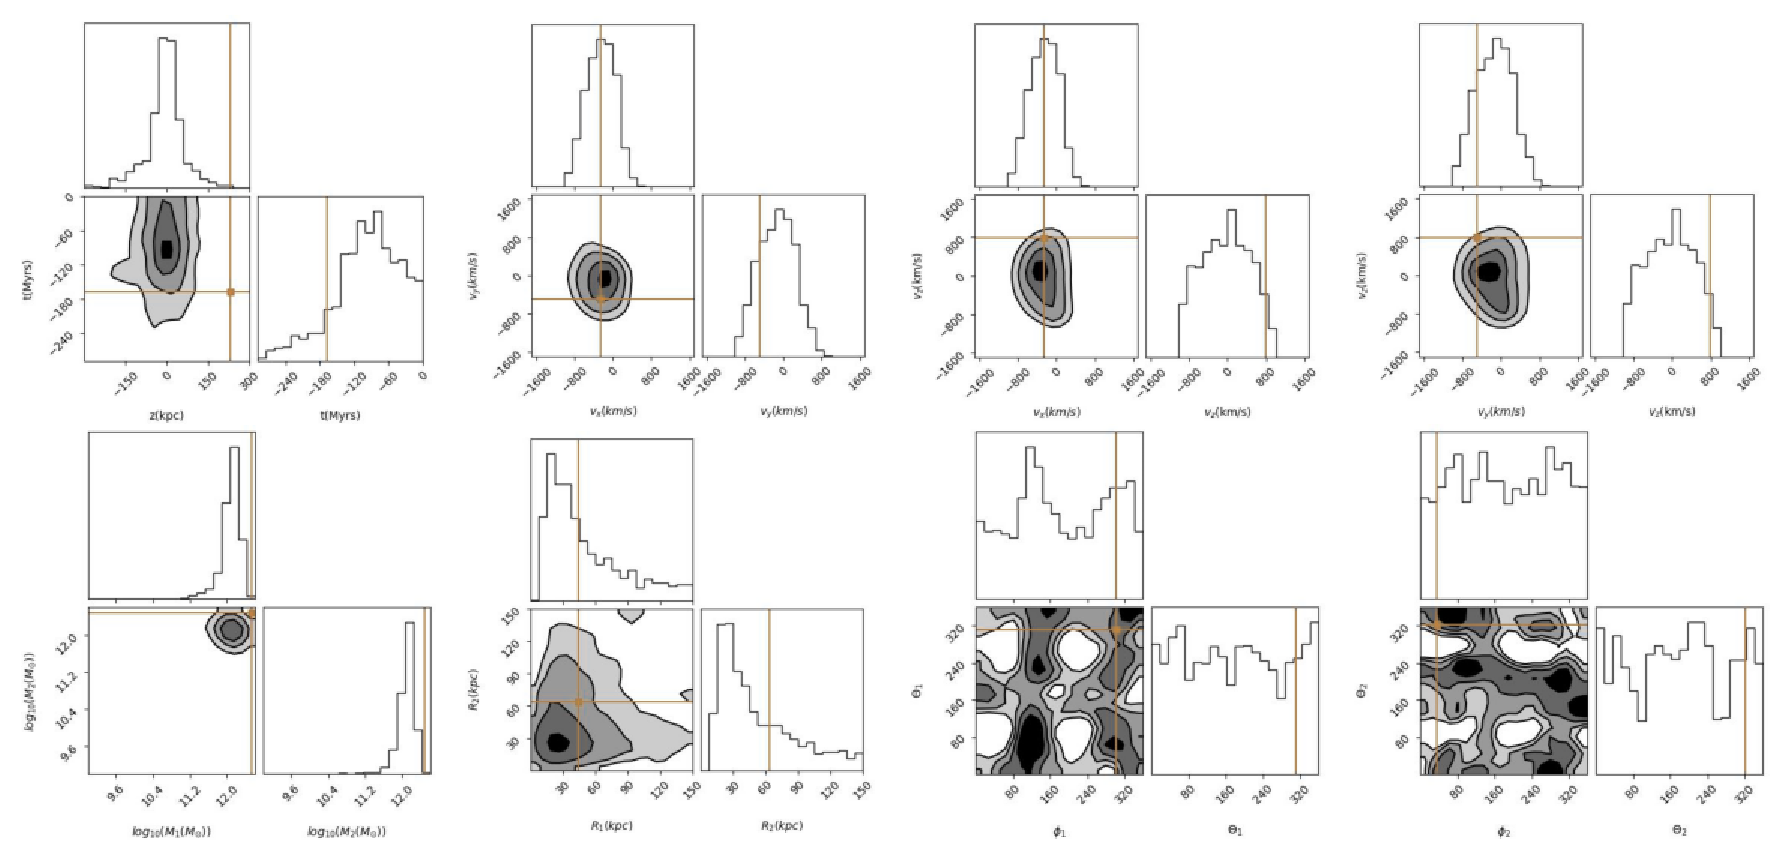
\includegraphics[width=\textwidth]{Chapter1/figures/Arp240_obs-red-corner.pdf}
    \caption[Reduced corner plot of the constraints made on the observational image of Arp 240.]{Reduced corner plot of the constraints made on the observational image of Arp 240. As shown, there is significant additional uncertainty in these measurements than those of the best fit simulation. However, we are able to make constraints on almost all parameters in the sample. The degeneracy in the orientations remains. The gold lines represent the true values we used in to create the synthetic image.}
    \label{fig:obs_corner_plot}
\end{figure*}

However, for the remainder of the parameters the level of constraint remains similar even with the change in the best fit values. We retain the two- and four-fold degeneracy in the orientation parameters. This follows on that the pipeline outright rejects disks which are edge on and loses accuracy when attempting to pin point the precise inclination of each galaxy. We are unable to make any constraint on the $\theta$ parameters, while the degeneracy of the $\phi$ parameters is still visible. The radius parameter is well constrained at 11.8\% CI, although with large tails in the probability space for both the primary and secondary galaxies. These tails are significantly larger here than when using the best fit simulation as the input. This is due to the observation image having no hard cutoff of the edge of the galaxy, and simply moving into more noise. The outer edges of our simulated galaxies also moves to very low signal, and therefore, there is lots of uncertainty surrounding the true radius of the galaxy. 

We, again, make excellent constraints on the mass parameters. The accuracy in the flux distribution of the primary and secondary disk is what dominates here, and therefore, we find this value incredibly quickly. The found value is comparable to the best fit simulation, although slightly lower. We also compare our constrained values to what is found in the literature. Using the criteria described previously, we recover total masses of $\frac{M_{1}}{10^{11}M_{\odot}} = 7.97 - 15.9$ and $\frac{M_{2}}{10^{11}M_{\odot}} = 8.1 - 16.2$ which correspond to stellar masses between $\frac{M_{1,*}}{10^{11}M_{\odot}} =  0.94 - 1.89$ and $\frac{M_{2, *}}{10^{11}M_{\odot}} = 1.0 - 1.9$ in our simulations. These are slightly higher than literature values, with a recent work quoting the stellar mass as $\frac{M_{1, *}}{10^{11}M_{\odot}} = 0.94 $ and $\frac{M_{2, *}}{10^{11}M_{\odot}} = 1.05$ \citep{2020MNRAS.496.5243H}. Thus, while our 50th percentile value is higher than the measured values, we do recover them within error.

This is true in the Arp 172 and Arp 290 observational constraints as well. The synthetic image we have used is at a different scale when compared to the the SDSS observations. We therefore end up with similar constraints to the different parameters, however with significant variation in the spatial parameters. The uncertainties in the radius parameters are significantly increased, while the constraint on the $\theta$ parameters is completely lost. In fact, for the same number of steps compared to constraining the best fit parameters, our MCMC fails the Geweke diagnostic. Therefore, due to the added noise running longer chains is imperative which drives up computational expense.

This leads us onto the limitations of this process to constraining galaxy interaction. While it has been very successful for many of the underlying parameters, there are many different parameters which must be provided to the pipeline so it is able to make those constraints. We discuss the limitations of applying this methodology to large interacting galaxy datasets, and how these can be offset in the short term but a long term solution is still required.

\subsection{Limitations}\label{limitations}
\noindent While this methodology does show a lot of promising in being able to constrain underlying parameters across populations of interacting galaxies, it is important to note that at its base is a restricted numerical interaction code with limited resolution. There may be some interacting systems that simply cannot be modelled realistically using three-body approximations, and may therefore cause a skew in results. However, there are also some more subtle limitations which may affect how a user wishes to use this MCMC approach.

\subsubsection{Resolution \& Depth Effects}\label{resolution_effect}
\noindent One of the fundamental parameters that must be provided for this methodology to work is the redshift of the system. This is used to calculate the distance to the system and then converted to an assumed resolution for the scale of the image. If this is input incorrectly the simulation images will be created at an incorrect resolution, and the MCMC will likely not reach convergence. This is also true of providing and calculating correctly an approximation of the position of the secondary galaxy. Significant computation power can be wasted if these parameters are incorrect, and will give spurious results. The reduction in resolution of the images is also an important limitation. This toy model needs small, thumbnail size images with a reasonable number of degrees of freedom as to reach convergence. Therefore, input images can only be of limited resolution which will affect the quality of the constraints we can actually make on different systems. 

The redshift is also used in scaling the fluxes calculated for each particle in the simulation. The base SED is calculated for a 1 M$_\odot$ system at a distance of 10pc. This is then scaled to the mass assigned to a particle and then put at the distance calculated from the redshift. If the redshift is incorrect (or even slightly off) then this could lead to a bad fit for the mass of the two galaxies in the system. A flag exists in the algorithm to give it the freedom to slightly vary the redshift (and therefore the distance and resolution) by 0.001 with each step. It will then attempt to fit the redshift and resolution of the system. Note, however, this is untested and currently significantly increases computational expense.

Depth effects also play a significant role in the ability of our algorithm to fit a system. For this work, we used primarily synthetic images, meaning we were not at risk of this. However, when using observational imaging this could become a significant problem. Our observational examples were of major interacting systems which resided in the high surface brightness regime, where we retained the full extent of the tidal features and could provide better fitting. However, for systems that lie closer to the low surface brightness regime, our algorithm will become less efficient and require more computational expense to make effective constraints.

This also has the opposite effect in terms of tidal features formed. For example, if a system is being fit but at the true parameters a tidal feature exists which has not been detected due to its low surface brightness then our MCMC pipeline will not be able to converge on the true values. The algorithm would instead converge on those parameters where the disks were at the correct flux rather than getting the tidal features correct. Therefore, when exploring the parameter space of interacting systems with our pipeline, it is imperative that the full structure is within detection of the observing instrument.

There must be a trade off between the resolution of our simulation and the observations. In this work, we used cutouts of 100 $\times$ 100 pixels. This was so that we could still get consistent system outputs from our simulations using only 2500 particles. If lots of pixels are used, then using a low number of particles can lead to many `unphysical' output simulations. I.e. these are simulation systems where the disks will have large holes in them where there haven't been enough particles to fill the disk. To mitigate the effect of potentially using low particle numbers, we distribute the flux as described in Section \ref{flux_dist}, which is an imperfect solution. It is recommended for any user to make a balanced trade off between resolution and computational expense.

\subsubsection{Computational Expense}\label{computational_expense}
\noindent The main drawback of this methodology is that of computational expense required to run such an MCMC over a the full parameter space. In the case of this work, the simulation was set up with 2500 particles on a High End Computer Cluster with 50 CPUS. Each simulation took approximately two seconds, with the full sample run taking approximately 30 days to complete. Each galaxy was given 600 walkers to move through parameter space with each walker moving 7,500 steps. The highest memory requirement of any system was 6GB. Therefore, the runtime is very high but the memory required for it is approximately 122MB per core.

This methodology was successful in constraining 51 different interacting galaxy synthetic images. Achieving the same in prior work projects, such as Galaxy Zoo: Mergers, took months to complete. We have reduced the runtime required of it to 30 days on a powerful High End Computer Cluster. However, this is not the solution to the large scale dataset problems that we will be seeing when LSST comes online. If we are to run this methodology on a much larger galaxy sample - such as thousands of galaxies - then we will need to find ways to significantly improve the runtime of this method.

\section{CONCLUSIONS \& FUTURE WORK}\label{Conclusions}
\noindent In this work, we have introduced a new algorithm based on a MCMC framework to apply constraints on the underlying parameters of interacting galaxies. We have made these constraints, and explored the underlying parameter space, through directly comparing input images to output simulations. Thus, we have mapped the underlying parameters that define interaction to an output morphology that we compare for similarity with a synthetic or observation image of an interaction. We have introduced an updated version of the restricted three body simulation JSPAM and modified it to calculate and match the flux distribution of interacting galaxies based on thirteen underlying parameters. This updated algorithm, APySPAM, calculates the flux distribution by assigning particles with a spectral energy distribution and accounting for star formation throughout the interaction. 

% Look at the tense mash up of the below paragraph.
To test our MCMC, we applied it to a set of synthetic images of interacting systems created from the parameters found in the Galaxy Zoo: Merger project for a set of real interacting systems. We were able to recover the true parameters used to create these images, with associated error measurements on each. We have explored the specific results of a single synthetic image: that of the Arp 240 system, and shown the corner plots and full posteriors of each parameter. We have took the 50th percentile value as the best fit value for our synthetic dataset, and used the 16th and 84th percentile to define the errors on our measurements. We then presented the distribution of our recovered underlying parameters and the true values, describing the general trends in our methodology as well as its limitations. 

Every parameter of our thirteen was recoverable, however there was significant degeneracy in the orientation angles of the two galactic disks. This was expected as works such as \citet{2010ASPC..423..227S} found significant degeneracy between systems, but not a direct cause. In this work we found, without taking account of kinematic information, multiple orientation angles can recreate observed tidal features as well as limitations in the pixel matching method of constraint. When tested on observational data of our best fit synthetic systems, we were able to retain the excellent constraints on nine of the thirteen parameters, but lost any constraint on the orientations. However, we were able to maintain a tight constraint on the masses of the two systems. 

There are limitations to this method that any users must be aware of. First, the core simulation of this process is a restricted three-body code with a highly optimised flux distribution calculation and approximation. It is probable that there are systems that this approach can not constrain, or may give nonphysical results for. The required reduction in the parameter space of the images, such as reducing the degrees of freedom and limiting individual pixel resolution in favour of computation time, also may lead to constraints only on the disks of the galaxies and not the tidal features themselves. There is also limited time and spatial resolution within the simulation itself. When using true observations, they had to be artificially scaled up so our simulation could maintain the resolution to have constraint. In terms of the temporal and spatial parameters, this scale up can be accounted for. However, in terms of the masses of the flux distribution, this can be significantly hindered. Therefore, a user must be careful when choosing the image scales to use when attempting to constrain individual systems. 

We have demonstrated the power of this methodology, and that it is capable of recovering the underlying parameters of interaction in idealised examples. The next, serious test of this MCMC approach will be to use it on a set of observed interacting systems, where the underlying parameters are known to properly diagnose the results. However, completely constrained interacting galaxy samples are only of a small scale and few exist. We will apply our MCMC to the observed dataset of our 51 interacting systems in SDSS.

This is an initial step towards developing the methodology to serve the field as large scale surveys - such as LSST - come online. Large scale automation where we can constrain interaction, make diagnostics and estimates about parameter space are not only important for inferences about individual datasets but for the interacting galaxy population as a whole. The main limitation of this method is the computational expense associated with it. To run this on 51 systems, the total run time was thirty days; an unusable timescale when being applied to interacting galaxy samples in the thousands. Therefore, future works with this algorithm and methodology will also be focused on increased computational efficiency and working on larger interacting galaxy datasets. 

The bottleneck for computational efficiency lies in the time spent running the APySPAM simulation. While incredibly cheap individually, this is exceptionally expensive when having to be run in an MCMC chain. With the growing power of GPUs, and their ability to run numerical simulations significantly more efficiently than CPUs, a pathway to solve this limitation may already exist. This, combined with further developments in methodologies such as simulation based inference, machine learning and gaussian processes could begin to reduce computation time.
\chapter{Summary and Future Work}\label{chapter:conclusion}
\section{Summary}
\noindent This work has focused on the role of galaxy interaction with respect to galaxy evolution. We have shown a new and novel way of creating large interacting galaxy samples, used it to explore the relation between galactic parameters and interaction and presented the initial pilot of a MCMC algorithm to definitively link the parameters of galaxies to the tidal features that form. The novel process of creating a large catalogue of interacting galaxies was detailed in Chapter \ref{chapter2}. By using newly developed data-access architecture with the newly developed Bayesian CNN, \texttt{Zoobot}, the largest catalogue of interacting galaxies to date was created. Along with this, we demonstrated how the new data-access architecture, ESA Datalabs, can be used to explore archival data volumes easily and efficiently. To make concrete links between galaxy evolution and interaction in the local volume, this catalogue was cross-matched to catalogues of ancillary data. This was done using the catalogues created from deep observations of the COSMOS field. This provided us with a flux limited sample of 4,181 and volume limited sample of 3,384, interacting galaxies to explore.

In Chapter \ref{chapter3} we conducted this exploration of our cross-matched sample in the context of interaction stage. We investigated whether conflicting theories about galaxy interaction were a result of not accounting for interaction stage based on observed morphology. We confirmed that interaction stage does have a significant impact on the underlying processes and enhancements that result from interaction. It was immediately found that the SFR increases dramatically through stage - from close pair to merger. This was demonstrated by measuring the distributions of stellar mass and SFR through stage and comparing them. We found that for distributions of stellar mass drawn from the same parent sample, the distribution of SFR changes. This was in the form of the disappearance of the red sequence, as our samples SFR was enhanced. We compared this with existing works which utilise the projected separation between systems as an approximation of the stage of interaction in the two systems. We found a complete disconnect with the projected separation and stage, noting that conflicting results can emerge from only looking at the projected separation without properly accounting for the interaction stage from the morphology. 

This degeneracy in the projected separation was particularly true of the change in the fraction of active galactic nuclei with stage, a topic the literature is particularly divided upon. We found that AGN fraction remained consistent with the field at 0.12 throughout the interaction, until coalescence where the fraction increased to 0.15. Breaking down our AGN counts with projected separation, we found two peaks in AGN count. Thus, this was not only evidence for AGN flickering, but also that there is some delay in the activation of the AGN which is difficult to account for when only using projected separation. While this methodology shows how we can use ancillary data to connect the underlying parameters of galaxies to interaction, and fundamental processes we attempted to conduct this in a more general way and to bring in linking to tidal feature formation. 

Chapter \ref{chapter4} saw the development of an algorithm to find the underlying parameters the galaxys' involved in interaction purely from their flux distribution. We combined a fast, efficient restricted numerical simulation with a MCMC methodology and Bayesian statistics and placed constraints on the underlying parameters of 51 synthetic images of interacting systems. While our uncertainties increased when applied to observational data, constraints were nonetheless able to be made upon the majority of the parameters. Constraints only failed on the orientation parameters. The creation of this MCMC algorithm paves the way to apply this to large interacting galaxy datasets such as the one described in Chapter \ref{chapter2}. However, the limitations in the runtime of the algorithm; taking approximately 15-20 hours per interacting galaxy, leads this to not be feasible. Therefore, methods of further improvement in efficiency of the underling numerical simulation must be explored. There is particular promise in this regard with the development of numerical simulations on GPUs, and the massive acceleration they provide to such projects.

We have created a large interacting galaxy dataset and demonstrated its capability in the context of how the progression of a galaxy changes the underlying properties of galaxies. We have introduced a method by which further examination of these systems could be explored, although further advances in its efficiency must be made for this approach to be viable. Potential methods, plus descriptions of future works in Chapters \ref{chapter2} and \ref{chapter3}, are discussed in the final subsection of this thesis.

\section{Future Work}
\subsection{Catalogues of Galaxy Morphology with Ancillary Data}
% Creating the largest catalogue of interacting galaxies has been done. Why not for all morphologies? Demonstrates the capability of ESA Datalabs. Mention this combination with Euclid, JWST and such.
\noindent Chapter \ref{chapter2} demonstrated that new data access architecture is now ready for us to conduct source classification at a scale rarely seen to this point. We can now directly access millions of sources across multiple filters, instruments and observatories to yield unprecedented sample sizes. These can be combined with novel machine learning algorithms requiring small training set sizes to fine-tune making them versatile and accurate across many different observatories. Since the publication of the paper underlaying Chapter \ref{chapter2}, the \texttt{Zoobot} algorithm has been updated many times. Not only is it now trained upon \textit{HST} data, but part of the representations of galaxies it learns is if a galaxy is interacting or not. By redoing the work conducted in Chapter \ref{chapter2}, one could classify galactic morphologies across the Galaxy Zoo workflow rather than just on an individual question.

The fundamental component of this which makes it possible is the ESA Datalabs platform. This platform has also been updated to provide access to many different observatories archives within it (such as \emph{JWST} and \emph{Euclid}) and also has access to much larger storage spaces and GPUs. Therefore, the entire work of Chapter \ref{chapter2} can be done on the platform with no requirement for data transfer (in our case, data had to be moved from ESA Datalabs to the Lancaster computer cluster for classification, taking the bulk of the project time). ESA Datalabs now allows us to conduct to a project similar to the one outlined in Chapter \ref{chapter2} with much greater efficiency. Not only could this classification be applied for interacting vs non-interacting, but we can also begin to consider creating larger catalogues of much broader morphology classifications. The recent Galaxy Zoo: DESI release contained 9.7 million galaxies with full morphology classification. Applying this to just the sources created in Chapter \ref{chapter2} would find 126 million morphology classifications, which is over a factor of 10 greater than previously achieved.

We can also take this further and not limit the opportunity here to only to only large catalogues of morphology classification. With the all-sky photometry that will be available from \emph{Euclid}, or survey scale photometry that will be available from ground based observatories like the Legacy Survey of Space and Time telescope, it will be possible to get broad-band photometry for millions of overlapping sources. By applying well-known astrophysical software such as \texttt{FAST}, \texttt{EAzY} or \texttt{LePhare}, it will be able to estimate many galactic parameters. These include the stellar masses, the photometric redshifts or, in some cases, the presence of AGN. By creating such large morphology catalogues, combined with this ancillary data, we will be able to robustly link different galaxy parameters to their physical morphologies. This can then be expanded out to include linking to the source environments across the sky. 

The development of algorithms like those proposed and tested in Chapter \ref{chapter4} will also provide excellent methods for constraining the underlying parameters of sources. While Chapter \ref{chapter4} focused on such an algorithm in the context of interacting galaxies, algorithms such as \texttt{GALFIT} are able to find morphological parameters purely from comparison to flux distributions and images. Even without further broad band photometry from other observatories, we will be able to explore the underlying parameter spaces of galaxies and link this to their morphologies using these data access architectures. 

\subsection{Constraining Interacting Galaxy Parameters}
% ALOT to talk about here. So, can discuss how GPUs are beginning to run numerical simulations with unprecedented efficiency. Talk about the rise in simulation based inference, and the easy transference of this pipeline to that. 
\noindent In Chapter \ref{chapter4}, we made direct links between the flux distribution of interacting galaxies and the parameters of those galaxies. We made constraints and revealed degeneracies across multiple parameters. However, the limitation of this approach was the computational expense, taking between 15-20 hours per system with the associated run time cost for this. For the large scale surveys or the catalogues such as those created in Chapter \ref{chapter2}, this efficiency is not enough. Making constraints on the entire sample selected in Chapter \ref{chapter2} would take between 37 and 50 years. However, there are multiple development routes that could be taken in future to boost computational efficiency. The first is to take full advantage of the next generation of GPUs. Many cases of accelerating numerical simulations have been written about and analysed, particularly from the GPU developer NVIDIA. These have demonstrated striking improvements in efficiency up to a factor of 3, especially in the context of numerical models of fluid dynamics \citep[recent examples include][]{Mantas2016, COSTA2021502}. Thus, reworking the code in this way would remove this limitation and have constraint being made in a matter of minutes: much more feasible for applying to large scale samples.

A second approach would be to move away from the direct method of MCMC and into utilising simulation based inference (SBI), often called likelihood free inference. Work has been conducted into SBI, and its massive increases in efficiency when constraining over large and complex parameter spaces \citep[for an excellent description of likelihood free inference, see][]{2021MNRAS.501..954J}. In this context, rather than running a MCMC and directly comparing simulation outputs to an observational image, a machine learning algorithm trained on simulation outputs is used to explore the parameter space. By running an initial set of simulations and feeding this into a rudimentary CNN, a low dimensional representative vector can be created of each image. This is then applied to the observational image. The CNN then approximates the posterior through parameter space, achieving constraints comparable to a direct MCMC exploration. However, while this approach has been very successful for small parameter spaces defining 1D cases, applying to cases of images - especially one defined by a 13D parameter space presented here - is in its infancy. 

Once this is evolved, however, it would succeed in significant improvements in the efficiency of our constraining algorithms. We could take advantage of the amortisation of SBI, and be able to apply our initially trained network and posterior distribution to many different systems instead of having to explore parameter space directly every time. This has the effect of front-loading the computational expense of our constraining process, running thousands to millions of simulations across parameter space initially to train the neural network and then being able to use the model in multiple cases, albeit with some caveats. Amortisation of the trained model across parameter space would be very sensitive to many different fundamental parts of our analysis process. For instance, changing the position of the secondary galaxy, the changing resolution of the images, the number of particles in the simulation, etc, all could be attempted. Changing any of these would mean amortisation is not valid, and the model would have to be retrained - re-introducing the problem of computational efficiency. 

However, if these caveats can be resolved, this would open the way for large-scale application of SBI and our direct inferencing methodology to large samples. These will be our next steps in the development of this algorithm, and to then make it widely accessible to the community, with the application of our sample of interacting galaxies from Chapter \ref{chapter2}. We will then be able to apply the process as conducted in Chapter \ref{chapter3}, and link the effects of interaction to further underlying parameters than the stellar mass, interaction stage and SFR.



%%%%%%%%%%%%%%%%%%%%%%%%%%%%%%%%%%%%%%%%%%%%%%%%%%%%%%%%%%%%%%%%%%%%%%%%%%%%%%%
% Appendices
%%%%%%%%%%%%%%%%%%%%%%%%%%%%%%%%%%%%%%%%%%%%%%%%%%%%%%%%%%%%%%%%%%%%%%%%%%%%%%%

\begin{appendices}
\chapter{Model Diagnostics \& Further Identified Objects}

\section{Further Model Diagnostics}\label{further-diagnostics}
\noindent In Section \ref{diagnostics} we present diagnostic properties of our model. These include the accuracy measurements, purity measurements as well as confusion matrices at different cutoffs of our model. Here, we present the Receiver Operating Characteristic (ROC) curves, the precision-recall (PR) curves, and measures of true and false positive rates vs the cutoff threshold.

Figure \ref{fig:pr-roc-curves} shows the ROC and PR curves of the final \texttt{Zoobot} model we applied to the the \emph{Hubble} archives. The ROC shows the rate of change of finding true positives and false positives with changing cutoff. The PR curve shows the changes of precision against recall. Precision is the ratio of true positives (interacting galaxies correctly predicted as so) to the sum of true and false positives (non-interacting galaxies incorrectly predicted as interacting). The recall is then the ratio of true positives to the sum of true positives and false negatives (interacting galaxies that have been misclassified as non-interacting). The red crosses in both plots shows how the model was behaving when we use a cutoff of 0.95. 

These are both as expected. Both curves show that the model behaves well, and are much better than a random classifier (which would have a 1:1 relation). The ROC plot shows that we are minimising our false positive rate when using a prediction score cutoff of 0.95. However, we are misclassifying approximately 50\% of interacting galaxies as non-interacting galaxies. The contamination rate in our final catalogue (False Positives rate) will be very low (close to zero in this ideal validation set). The PR curve shows a similar result. Here, we are operating with a high precision (finding a pure catalogue) while keeping our recall minimal. 

We also present the changing F1 score for the model used in this work, shown in Figure \ref{fig:f1-score}. The F1 score is twice the ratio of precision multiplied by recall upon precision summed to recall. This combines our measure of accuracy and purity into a single metric. The cutoff we use in this work is at the point where the F1 score has began to decline. This is because we are beginning to lose recall rapidly, but gaining significantly in precision. As discussed in Section \ref{diagnostics}, this was an acceptable trade off in this work for a very large, pure interacting galaxy catalogue.

\begin{figure*}
  \centering
  \includegraphics[width = 0.95\textwidth]{Chapter2/figures/fig14.jpg}
  \caption{The Receiver-Operator and Precision-Recall Curve for the \texttt{Zoobot} model that was used to explore the Hubble archives. The blue curves are the measured curves. These curves measure the relevant rates or characteristics based on the changing cutoff applied to how \texttt{Zoobot} defines an interacting galaxy. The red crosses are where the prediction score cutoff is for this work. We can see in the Reciever-Operator Curve that the prediction score cutoff we use would have an incredibly low false positive rate, while it would be misclassifying $\approx$50\% of interacting galaxies. This also shown in the precision recall curve where our recall is $\approx$50\%.}
  \label{fig:pr-roc-curves}
\end{figure*}

\begin{figure*}
    \centering
    \includegraphics[width = 0.65\textwidth]{Chapter2/figures/fig15.pdf}
    \caption{The F1 score found during the diagnostics of the model used in this work. The F1 score is a measure combing the measure of accuracy and purity into one metric. The cutoff we use is at the point where the F1 score begins to rapidly decline. This point is shown by the red vertical line.}
    \label{fig:f1-score}
\end{figure*}

\section{Examples of Sources with 3-Band Information}\label{colour-images}
\noindent Of the full catalogue of 21,926 interacting systems, only 1336 of them had got all 3-band information. Six examples are shown in Figure \ref{fig:colour-images}. These were created using the \citet{lupton_04} algorithm, with a scaling factor $Q = 2$ and $\alpha = 0.75$, with ($F814W$, $F606W$, $F475W$) as RGB channels and multiplicative factors of (1.25, 0.95, 2).

\begin{figure*}
  \centering
  \includegraphics[width = 0.85\textwidth]{Chapter2/figures/fig16.jpeg}
  \caption{Example of six interacting systems in the catalogue with full 3-band imagery.}
  \label{fig:colour-images}
\end{figure*}

\section{Unknown Objects}\label{unknown-object}
\noindent From the final catalogue, there were six sources which we could not visually identify. These objects were also not referenced anywhere in the astrophysical literature. $F814W$ cutouts of the six objects are shown in Figure \ref{fig:unknown-images}. Their Source IDs are shown in the upper left of each image, and a separate catalogue has been released of these with all other objects. This catalogue can be found at the data release on Zenodo.

Four of the six objects (40001156424176, 4001368788120, 4001418076626 and 6000398415347) have a bright central source, followed by a low-surface brightness tail. Initially, it was assumed that these were solar system objects such as comets. This, however, could not be confirmed. The first of these four sources is also thought to potentially be a highly disruped system with a significantly elongated tidal feature. The final two unknown sources (6000186797547 and 6000341449179) have no clear central source, though there is extended structure to them. These are likely to be highly irregular galaxies, but no confirmation could be found.

These objects are released to the community for identification and investigation, as the authors cannot find definitive agreement on what they are. 

\begin{figure*}
  \centering
  \includegraphics[width = 0.85\textwidth]{Chapter2/figures/fig17.pdf}
  \caption{The six unknown systems found in this work. These have no reference in Simbad or in NED, and their morphology could not be classified by the authors. Investigation into these six objects are presented to the community, with the authors hoping that future work and investigation of them can be conducted by them.}
  \label{fig:unknown-images}
\end{figure*}

\section{Acknowledging PIs}
\noindent In the final section of this work, we wish to acknowledge all of the PIs whose observations we have used. A machine readable table containing the proposal IDs, the DOIs and the references (if provided/found) is presented with this work. Table \ref{tab:pis} shows the first twenty observations used in this work and is an example of this table.

\begin{table}
\centering
	\begin{tabular}{ccccc}
	Proposal ID & Observation ID & Observation Date & DOI & references \\
	    8183       &   hst\_8183\_54\_acs\_wfc\_f814w\_j59l54 &       18/07/2002 &    https://doi.org/10.5270/esa-88k8vcj & \\
	    9075       &   hst\_9075\_2a\_acs\_wfc\_f814w\_j6fl2a &       24/07/2002 &    https://doi.org/10.5270/esa-gsxhb4b & \\
	    9351       &   hst\_9351\_11\_acs\_wfc\_f814w\_j8d211 &       31/03/2003 &    https://doi.org/10.5270/esa-5lba8bo & \\
	    9361       &   hst\_9361\_03\_acs\_wfc\_f814w\_j8d503 &       22/07/2003 &    https://doi.org/10.5270/esa-ecmnqgh & \\
	    9363       &   hst\_9363\_09\_acs\_wfc\_f814w\_j8d809 &       02/07/2002 &    https://doi.org/10.5270/esa-ethtec5 & \\
	    9367       &   hst\_9367\_02\_acs\_wfc\_f814w\_j8ds02 &       10/06/2003 &    https://doi.org/10.5270/esa-3j404ll & \\
	    9373       &   hst\_9373\_02\_acs\_wfc\_f814w\_j6la02 &       05/07/2002 &    https://doi.org/10.5270/esa-ztsq94u & \citet{Rejkuba_05}\\
	    9376       &   hst\_9376\_02\_acs\_wfc\_f814w\_j8e302 &       13/07/2002 &    https://doi.org/10.5270/esa-h90iavd & \citet{Keel06}\\
	    9381       &   hst\_9381\_02\_acs\_wfc\_f814w\_j8fu02 &       13/03/2003 &    https://doi.org/10.5270/esa-vlapyea & \\
	    9400       &   hst\_9400\_04\_acs\_wfc\_f814w\_j6kx04 &       29/05/2003 &    https://doi.org/10.5270/esa-39rnout & \\
	    9403       &   hst\_9403\_02\_acs\_wfc\_f814w\_j8fp02 &       09/07/2002 &    https://doi.org/10.5270/esa-k5mv9ct & \\
	    9405       &   hst\_9405\_6k\_acs\_wfc\_f814w\_j8iy6k &       22/05/2003 &    https://doi.org/10.5270/esa-zy9phm1 & \\
	    9409       &   hst\_9409\_03\_acs\_wfc\_f814w\_j6n203 &       29/06/2003 &    https://doi.org/10.5270/esa-vjngw7r & \citet{goudfrooij04}\\
	    9411       &   hst\_9411\_09\_acs\_wfc\_f814w\_j8dl09 &       11/02/2003 &    https://doi.org/10.5270/esa-debpiln &  \\
	    9427       &   hst\_9427\_13\_acs\_wfc\_f814w\_j6m613 &       21/10/2002 &    https://doi.org/10.5270/esa-bw1b97v &  \\
	    9438       &   hst\_9438\_01\_acs\_wfc\_f814w\_j6me01 &       16/01/2003 &    https://doi.org/10.5270/esa-e5eaam5 & \citet{gregg17}\\
	    9450       &   hst\_9450\_02\_acs\_wfc\_f814w\_j8d402 &       25/08/2002 &    https://doi.org/10.5270/esa-9ttmykz & \citet{york05}\\
	    9453       &   hst\_9453\_02\_acs\_wfc\_f814w\_j8f802 &       03/12/2002 &    https://doi.org/10.5270/esa-1xvyjfy & \citet{brown03}\\
	    9454       &   hst\_9454\_11\_acs\_wfc\_f814w\_j8ff11 &       23/03/2003 &    https://doi.org/10.5270/esa-xsdowj9 &  \\
	\end{tabular}
\caption{Twenty example of the accompanying data table of observations used.} 
\label{tab:pis}
\end{table}
\chapter{Model Diagnostics \& Further Identified Objects}

\section{Further Model Diagnostics}\label{further-diagnostics}
\noindent In Section \ref{diagnostics} we present diagnostic properties of our model. These include the accuracy measurements, purity measurements as well as confusion matrices at different cutoffs of our model. Here, we present the Receiver Operating Characteristic (ROC) curves, the precision-recall (PR) curves, and measures of true and false positive rates vs the cutoff threshold.

Figure \ref{fig:pr-roc-curves} shows the ROC and PR curves of the final \texttt{Zoobot} model we applied to the the \emph{Hubble} archives. The ROC shows the rate of change of finding true positives and false positives with changing cutoff. The PR curve shows the changes of precision against recall. Precision is the ratio of true positives (interacting galaxies correctly predicted as so) to the sum of true and false positives (non-interacting galaxies incorrectly predicted as interacting). The recall is then the ratio of true positives to the sum of true positives and false negatives (interacting galaxies that have been misclassified as non-interacting). The red crosses in both plots shows how the model was behaving when we use a cutoff of 0.95. 

These are both as expected. Both curves show that the model behaves well, and are much better than a random classifier (which would have a 1:1 relation). The ROC plot shows that we are minimising our false positive rate when using a prediction score cutoff of 0.95. However, we are misclassifying approximately 50\% of interacting galaxies as non-interacting galaxies. The contamination rate in our final catalogue (False Positives rate) will be very low (close to zero in this ideal validation set). The PR curve shows a similar result. Here, we are operating with a high precision (finding a pure catalogue) while keeping our recall minimal. 

We also present the changing F1 score for the model used in this work, shown in Figure \ref{fig:f1-score}. The F1 score is twice the ratio of precision multiplied by recall upon precision summed to recall. This combines our measure of accuracy and purity into a single metric. The cutoff we use in this work is at the point where the F1 score has began to decline. This is because we are beginning to lose recall rapidly, but gaining significantly in precision. As discussed in Section \ref{diagnostics}, this was an acceptable trade off in this work for a very large, pure interacting galaxy catalogue.

\begin{figure*}
  \centering
  \includegraphics[width = 0.95\textwidth]{Chapter2/figures/fig14.jpg}
  \caption{The Receiver-Operator and Precision-Recall Curve for the \texttt{Zoobot} model that was used to explore the Hubble archives. The blue curves are the measured curves. These curves measure the relevant rates or characteristics based on the changing cutoff applied to how \texttt{Zoobot} defines an interacting galaxy. The red crosses are where the prediction score cutoff is for this work. We can see in the Reciever-Operator Curve that the prediction score cutoff we use would have an incredibly low false positive rate, while it would be misclassifying $\approx$50\% of interacting galaxies. This also shown in the precision recall curve where our recall is $\approx$50\%.}
  \label{fig:pr-roc-curves}
\end{figure*}

\begin{figure*}
    \centering
    \includegraphics[width = 0.65\textwidth]{Chapter2/figures/fig15.pdf}
    \caption{The F1 score found during the diagnostics of the model used in this work. The F1 score is a measure combing the measure of accuracy and purity into one metric. The cutoff we use is at the point where the F1 score begins to rapidly decline. This point is shown by the red vertical line.}
    \label{fig:f1-score}
\end{figure*}

\section{Examples of Sources with 3-Band Information}\label{colour-images}
\noindent Of the full catalogue of 21,926 interacting systems, only 1336 of them had got all 3-band information. Six examples are shown in Figure \ref{fig:colour-images}. These were created using the \citet{lupton_04} algorithm, with a scaling factor $Q = 2$ and $\alpha = 0.75$, with ($F814W$, $F606W$, $F475W$) as RGB channels and multiplicative factors of (1.25, 0.95, 2).

\begin{figure*}
  \centering
  \includegraphics[width = 0.85\textwidth]{Chapter2/figures/fig16.jpeg}
  \caption{Example of six interacting systems in the catalogue with full 3-band imagery.}
  \label{fig:colour-images}
\end{figure*}

\section{Unknown Objects}\label{unknown-object}
\noindent From the final catalogue, there were six sources which we could not visually identify. These objects were also not referenced anywhere in the astrophysical literature. $F814W$ cutouts of the six objects are shown in Figure \ref{fig:unknown-images}. Their Source IDs are shown in the upper left of each image, and a separate catalogue has been released of these with all other objects. This catalogue can be found at the data release on Zenodo.

Four of the six objects (40001156424176, 4001368788120, 4001418076626 and 6000398415347) have a bright central source, followed by a low-surface brightness tail. Initially, it was assumed that these were solar system objects such as comets. This, however, could not be confirmed. The first of these four sources is also thought to potentially be a highly disruped system with a significantly elongated tidal feature. The final two unknown sources (6000186797547 and 6000341449179) have no clear central source, though there is extended structure to them. These are likely to be highly irregular galaxies, but no confirmation could be found.

These objects are released to the community for identification and investigation, as the authors cannot find definitive agreement on what they are. 

\begin{figure*}
  \centering
  \includegraphics[width = 0.85\textwidth]{Chapter2/figures/fig17.pdf}
  \caption{The six unknown systems found in this work. These have no reference in Simbad or in NED, and their morphology could not be classified by the authors. Investigation into these six objects are presented to the community, with the authors hoping that future work and investigation of them can be conducted by them.}
  \label{fig:unknown-images}
\end{figure*}

\section{Acknowledging PIs}
\noindent In the final section of this work, we wish to acknowledge all of the PIs whose observations we have used. A machine readable table containing the proposal IDs, the DOIs and the references (if provided/found) is presented with this work. Table \ref{tab:pis} shows the first twenty observations used in this work and is an example of this table.

\begin{table}
\centering
	\begin{tabular}{ccccc}
	Proposal ID & Observation ID & Observation Date & DOI & references \\
	    8183       &   hst\_8183\_54\_acs\_wfc\_f814w\_j59l54 &       18/07/2002 &    https://doi.org/10.5270/esa-88k8vcj & \\
	    9075       &   hst\_9075\_2a\_acs\_wfc\_f814w\_j6fl2a &       24/07/2002 &    https://doi.org/10.5270/esa-gsxhb4b & \\
	    9351       &   hst\_9351\_11\_acs\_wfc\_f814w\_j8d211 &       31/03/2003 &    https://doi.org/10.5270/esa-5lba8bo & \\
	    9361       &   hst\_9361\_03\_acs\_wfc\_f814w\_j8d503 &       22/07/2003 &    https://doi.org/10.5270/esa-ecmnqgh & \\
	    9363       &   hst\_9363\_09\_acs\_wfc\_f814w\_j8d809 &       02/07/2002 &    https://doi.org/10.5270/esa-ethtec5 & \\
	    9367       &   hst\_9367\_02\_acs\_wfc\_f814w\_j8ds02 &       10/06/2003 &    https://doi.org/10.5270/esa-3j404ll & \\
	    9373       &   hst\_9373\_02\_acs\_wfc\_f814w\_j6la02 &       05/07/2002 &    https://doi.org/10.5270/esa-ztsq94u & \citet{Rejkuba_05}\\
	    9376       &   hst\_9376\_02\_acs\_wfc\_f814w\_j8e302 &       13/07/2002 &    https://doi.org/10.5270/esa-h90iavd & \citet{Keel06}\\
	    9381       &   hst\_9381\_02\_acs\_wfc\_f814w\_j8fu02 &       13/03/2003 &    https://doi.org/10.5270/esa-vlapyea & \\
	    9400       &   hst\_9400\_04\_acs\_wfc\_f814w\_j6kx04 &       29/05/2003 &    https://doi.org/10.5270/esa-39rnout & \\
	    9403       &   hst\_9403\_02\_acs\_wfc\_f814w\_j8fp02 &       09/07/2002 &    https://doi.org/10.5270/esa-k5mv9ct & \\
	    9405       &   hst\_9405\_6k\_acs\_wfc\_f814w\_j8iy6k &       22/05/2003 &    https://doi.org/10.5270/esa-zy9phm1 & \\
	    9409       &   hst\_9409\_03\_acs\_wfc\_f814w\_j6n203 &       29/06/2003 &    https://doi.org/10.5270/esa-vjngw7r & \citet{goudfrooij04}\\
	    9411       &   hst\_9411\_09\_acs\_wfc\_f814w\_j8dl09 &       11/02/2003 &    https://doi.org/10.5270/esa-debpiln &  \\
	    9427       &   hst\_9427\_13\_acs\_wfc\_f814w\_j6m613 &       21/10/2002 &    https://doi.org/10.5270/esa-bw1b97v &  \\
	    9438       &   hst\_9438\_01\_acs\_wfc\_f814w\_j6me01 &       16/01/2003 &    https://doi.org/10.5270/esa-e5eaam5 & \citet{gregg17}\\
	    9450       &   hst\_9450\_02\_acs\_wfc\_f814w\_j8d402 &       25/08/2002 &    https://doi.org/10.5270/esa-9ttmykz & \citet{york05}\\
	    9453       &   hst\_9453\_02\_acs\_wfc\_f814w\_j8f802 &       03/12/2002 &    https://doi.org/10.5270/esa-1xvyjfy & \citet{brown03}\\
	    9454       &   hst\_9454\_11\_acs\_wfc\_f814w\_j8ff11 &       23/03/2003 &    https://doi.org/10.5270/esa-xsdowj9 &  \\
	\end{tabular}
\caption{Twenty example of the accompanying data table of observations used.} 
\label{tab:pis}
\end{table}
\end{appendices}


%\backmatter
%%%%%%%%%%%%%%%%%%%%%%%%%%%%%%%%%%%%%%%%%%%%%%%%%%%%%%%%%%%%%%%%%%%%%%%%%%%%%%%
% bibliography
%%%%%%%%%%%%%%%%%%%%%%%%%%%%%%%%%%%%%%%%%%%%%%%%%%%%%%%%%%%%%%%%%%%%%%%%%%%%%%%

%\nocite{} %use while references are not cited
\renewcommand{\bibname}{References}

\bibliographystyle{Latex/mnras}  %use the plain bibliography style
\bibliography{thesis}        %use a bibtex bibliography file thesis.bib

\end{document}
